\documentclass[a4paper,14pt,oneside,openany]{memoir}

%%% Задаем поля, отступы и межстрочный интервал %%%

\usepackage[left=30mm, right=15mm, top=20mm, bottom=20mm]{geometry} % Пакет geometry с аргументами для определения полей
\pagestyle{plain} % Убираем стандарные для данного класса верхние колонтитулы с заголовком текущей главы, оставляем только номер страницы снизу по центру
\parindent=1.25cm % Абзацный отступ 1.25 см, приблизительно равно пяти знакам, как по ГОСТ
\usepackage{indentfirst} % Добавляем отступ к первому абзацу
%\linespread{1.3} % Межстрочный интервал (наиболее близко к вордовскому полуторному) - тут вместо этого используется команда OnehalfSpacing*

%%% Задаем языковые параметры и шрифт %%%

\usepackage[english, russian]{babel}                % Настройки для русского языка как основного в тексте
\babelfont{rm}{Times New Roman}                     % TMR в качестве базового roman-щрифта

%%% Задаем стиль заголовков и подзаголовков в тексте %%%

\setsecnumdepth{subsection} % Номера разделов считать до третьего уровня включительно, т.е. нумеруются только главы, секции, подсекции
\renewcommand*{\chapterheadstart}{} % Переопределяем команду, задающую отступ над заголовком, чтобы отступа не было
\renewcommand*{\printchaptername}{} % Переопределяем команду, печатающую слово "Глава", чтобы оно не печалось
%\renewcommand*{\printchapternum}{} % То же самое для номера главы - тут не надо, номер главы оставляем
\renewcommand*{\chapnumfont}{\normalfont\bfseries} % Меняем стиль шрифта для номера главы: нормальный размер, полужирный
\renewcommand*{\afterchapternum}{\hspace{1em}} % Меняем разделитель между номером главы и названием
\renewcommand*{\printchaptertitle}{\normalfont\bfseries\centering\MakeUppercase} % Меняем стиль написания для заголовка главы: нормальный размер, полужирный, центрированный, заглавными буквами
\setbeforesecskip{20pt} % Задаем отступ перед заголовком секции
\setaftersecskip{20pt} % Ставим такой же отступ после заголовка секции
\setsecheadstyle{\raggedright\normalfont\bfseries} % Меняем стиль написания для заголовка секции: выравнивание по правому краю без переносов, нормальный размер, полужирный
\setbeforesubsecskip{20pt} % Задаем отступ перед заголовком подсекции
\setaftersubsecskip{20pt} % Ставим такой же отступ после заголовка подсекции
\setsubsecheadstyle{\raggedright\normalfont\bfseries}  % Меняем стиль написания для заголовка подсекции: выравнивание по правому краю без переносов, нормальный размер, полужирный

%%% Задаем параметры оглавления %%%

\addto\captionsrussian{\renewcommand\contentsname{Содержание}} % Меняем слово "Оглавление" на "Содержание"
\setrmarg{2.55em plus1fil} % Запрещаем переносы слов в оглавлении
%\setlength{\cftbeforechapterskip}{0pt} % Эта команда убирает интервал между заголовками глав - тут не надо, так красивее смотрится
\renewcommand{\aftertoctitle}{\afterchaptertitle \vspace{-\cftbeforechapterskip}} % Делаем отступ между словом "Содержание" и первой строкой таким же, как у заголовков глав
%\renewcommand*{\chapternumberline}[1]{} % Делаем так, чтобы номер главы не печатался - тут не надо
\renewcommand*{\cftchapternumwidth}{1.5em} % Ставим подходящий по размеру разделитель между номером главы и самим заголовком
\renewcommand*{\cftchapterfont}{\normalfont\MakeUppercase} % Названия глав обычным шрифтом заглавными буквами
\renewcommand*{\cftchapterpagefont}{\normalfont} % Номера страниц обычным шрифтом
\renewcommand*{\cftchapterdotsep}{\cftdotsep} % Делаем точки до номера страницы после названий глав
\renewcommand*{\cftdotsep}{1} % Задаем расстояние между точками
\renewcommand*{\cftchapterleader}{\cftdotfill{\cftchapterdotsep}} % Делаем точки стандартной формы (по умолчанию они "жирные")
\maxtocdepth{subsection} % В оглавление попадают только разделы первыхтрех уровней: главы, секции и подсекции

%%% Выравнивание и переносы %%%

%% http://tex.stackexchange.com/questions/241343/what-is-the-meaning-of-fussy-sloppy-emergencystretch-tolerance-hbadness
%% http://www.latex-community.org/forum/viewtopic.php?p=70342#p70342
\tolerance 1414
\hbadness 1414
\emergencystretch 1.5em                             % В случае проблем регулировать в первую очередь
\hfuzz 0.3pt
\vfuzz \hfuzz
%\dbottom
%\sloppy                                            % Избавляемся от переполнений
\clubpenalty=10000                                  % Запрещаем разрыв страницы после первой строки абзаца
\widowpenalty=10000                                 % Запрещаем разрыв страницы после последней строки абзаца
\brokenpenalty=4991                                 % Ограничение на разрыв страницы, если строка заканчивается переносом

%%% Объясняем компилятору, какие буквы русского алфавита можно использовать в перечислениях (подрисунках и нумерованных списках) %%%
%%% По ГОСТ нельзя использовать буквы ё, з, й, о, ч, ь, ы, ъ %%%
%%% Здесь также переопределены заглавные буквы, хотя в принципе они в документе не используются %%%

\makeatletter
    \def\russian@Alph#1{\ifcase#1\or
       А\or Б\or В\or Г\or Д\or Е\or Ж\or
       И\or К\or Л\or М\or Н\or
       П\or Р\or С\or Т\or У\or Ф\or Х\or
       Ц\or Ш\or Щ\or Э\or Ю\or Я\else\xpg@ill@value{#1}{russian@Alph}\fi}
    \def\russian@alph#1{\ifcase#1\or
       а\or б\or в\or г\or д\or е\or ж\or
       и\or к\or л\or м\or н\or
       п\or р\or с\or т\or у\or ф\or х\or
       ц\or ш\or щ\or э\or ю\or я\else\xpg@ill@value{#1}{russian@alph}\fi}
\makeatother

%%% Задаем параметры оформления рисунков и таблиц %%%

\usepackage{graphicx, caption, subcaption} % Подгружаем пакеты для работы с графикой и настройки подписей
\graphicspath{{images/}} % Определяем папку с рисунками
\captionsetup[figure]{font=small, width=\textwidth, name=Рисунок, justification=centering} % Задаем параметры подписей к рисункам: маленький шрифт (в данном случае 12pt), ширина равна ширине текста, полнотекстовая надпись "Рисунок", выравнивание по центру
\captionsetup[subfigure]{font=small} % Индексы подрисунков а), б) и так далее тоже шрифтом 12pt (по умолчанию делает еще меньше)
\captionsetup[table]{singlelinecheck=false,font=small,width=\textwidth,justification=justified} % Задаем параметры подписей к таблицам: запрещаем переносы, маленький шрифт (в данном случае 12pt), ширина равна ширине текста, выравнивание по ширине
\captiondelim{ --- } % Разделителем между номером рисунка/таблицы и текстом в подписи является длинное тире
\setkeys{Gin}{width=\textwidth} % По умолчанию размер всех добавляемых рисунков будет подгоняться под ширину текста
\renewcommand{\thesubfigure}{\asbuk{subfigure}} % Нумерация подрисунков строчными буквами кириллицы
%\setlength{\abovecaptionskip}{0pt} % Отбивка над подписью - тут не меняем
%\setlength{\belowcaptionskip}{0pt} % Отбивка под подписью - тут не меняем
\usepackage[section]{placeins} % Объекты типа float (рисунки/таблицы) не вылезают за границы секциии, в которой они объявлены

%%% Задаем параметры ссылок и гиперссылок %%% 

\usepackage{hyperref}                               % Подгружаем нужный пакет
\hypersetup{
    colorlinks=true,                                % Все ссылки и гиперссылки цветные
    linktoc=all,                                    % В оглавлении ссылки подключатся для всех отображаемых уровней
    linktocpage=true,                               % Ссылка - только номер страницы, а не весь заголовок (так выглядит аккуратнее)
    linkcolor=red,                                  % Цвет ссылок и гиперссылок - красный
    citecolor=red                                   % Цвет цитировний - красный
}

%%% Настраиваем отображение списков %%%

\usepackage{enumitem}                               % Подгружаем пакет для гибкой настройки списков
\renewcommand*{\labelitemi}{\normalfont{--}}        % В ненумерованных списках для пунктов используем короткое тире
\makeatletter
    \AddEnumerateCounter{\asbuk}{\russian@alph}     % Объясняем пакету enumitem, как использовать asbuk
\makeatother
\renewcommand{\labelenumii}{\asbuk{enumii})}        % Кириллица для второго уровня нумерации
\renewcommand{\labelenumiii}{\arabic{enumiii})}     % Арабские цифры для третьего уровня нумерации
\setlist{noitemsep, leftmargin=*}                   % Убираем интервалы между пунками одного уровня в списке
\setlist[1]{labelindent=\parindent}                 % Отступ у пунктов списка равен абзацному отступу
\setlist[2]{leftmargin=\parindent}                  % Плюс еще один такой же отступ для следующего уровня
\setlist[3]{leftmargin=\parindent}                  % И еще один для третьего уровня

%%% Счетчики для нумерации объектов %%%

\counterwithout{figure}{chapter}                    % Сквозная нумерация рисунков по документу
\counterwithout{equation}{chapter}                  % Сквозная нумерация математических выражений по документу
\counterwithout{table}{chapter}                     % Сквозная нумерация таблиц по документу

%%% Реализация библиографии пакетами biblatex и biblatex-gost с использованием движка biber %%%

\usepackage{csquotes} % Пакет для оформления сложных блоков цитирования (biblatex рекомендует его подключать)
\usepackage[%
backend=biber,                                      % Движок
bibencoding=utf8,                                   % Кодировка bib-файла
sorting=none,                                       % Настройка сортировки списка литературы
style=gost-numeric,                                 % Стиль цитирования и библиографии по ГОСТ
language=auto,                                      % Язык для каждой библиографической записи задается отдельно
autolang=other,                                     % Поддержка многоязычной библиографии
sortcites=true,                                     % Если в квадратных скобках несколько ссылок, то отображаться будут отсортированно
movenames=false,                                    % Не перемещать имена, они всегда в начале библиографической записи
maxnames=5,                                         % Максимальное отображаемое число авторов
minnames=3,                                         % До скольки сокращать число авторов, если их больше максимума
doi=false,                                          % Не отображать ссылки на DOI
isbn=false,                                         % Не показывать ISBN, ISSN, ISRN
]{biblatex}[2016/09/17]
\DeclareDelimFormat{bibinitdelim}{}                 % Убираем пробел между инициалами (Иванов И.И. вместо Иванов И. И.)
\addbibresource{biba.bib}                           % Определяем файл с библиографией

%%% Скрипт, который автоматически подбирает язык (и, следовательно, формат) для каждой библиографической записи %%%
%%% Если в названии работы есть кириллица - меняем значение поля langid на russian %%%
%%% Все оставшиеся пустые места в поле langid заменяем на english %%%

\DeclareSourcemap{
  \maps[datatype=bibtex]{
    \map{
        \step[fieldsource=title, match=\regexp{^\P{Cyrillic}*\p{Cyrillic}.*}, final]
        \step[fieldset=langid, fieldvalue={russian}]
    }
    \map{
        \step[fieldset=langid, fieldvalue={english}]
    }
  }
}

%%% Прочие пакеты для расширения функционала %%%

\usepackage{longtable,ltcaption}                    % Длинные таблицы
\usepackage{multirow,makecell}                      % Улучшенное форматирование таблиц
\usepackage{booktabs}                               % Еще один пакет для красивых таблиц
\usepackage{soulutf8}                               % Поддержка переносоустойчивых подчёркиваний и зачёркиваний
\usepackage{icomma}                                 % Запятая в десятичных дробях
\usepackage{hyphenat}                               % Для красивых переносов
\usepackage{textcomp}                               % Поддержка "сложных" печатных символов типа значков иены, копирайта и т.д.
\usepackage[version=4]{mhchem}                      % Красивые химические уравнения
\usepackage{amsmath}                                % Усовершенствование отображения математических выражений 

%%% Вставляем по очереди все содержательные части документа %%%

\begin{document}

\thispagestyle{empty}

\begin{center}
    МИНИСТЕРСТВО НАУКИ И ВЫСШЕГО ОБРАЗОВАНИЯ \\ РОССИЙСКОЙ ФЕДЕРАЦИИ

    \vspace{20pt}

    Федеральное государственное автономное \\ образовательное учреждение высшего образования \\
    "<Национальный исследовательский университет ИТМО"> \\
    (Университет ИТМО)

    \vspace{20pt}

    Факультет систем управления и робототехники 
\end{center}

\vfill

\begin{center}
    ОТЧЕТ \\  
    по Курсовому проекту: \\
    \uppercase{Управление перевернутым маятником на тележке}
    \vspace{20pt}
    
    Вариант 17 \\

    \vspace{20pt}
    
    по дисциплине \\
    \textit{"<Теория автоматического управления">}

\end{center}

\vfill

    \noindent Студент: \\
    \textit{Группа № R3338 \hfill А.А. Нечаева}

    \vspace{20pt}

    \noindent Предподаватель: \\
    \textit{ассистент факультера СУиР, к. т. н. \hfill А.В. Пашенко}

\vfill

\begin{center}
    Санкт-Петербург 2025
\end{center}                                     % Титульник

\newpage % Переходим на новую страницу
\setcounter{page}{2} % Начинаем считать номера страниц со второй
\OnehalfSpacing* % Задаем полуторный интервал текста (в титульнике одинарный, поэтому команда стоит после него)

\tableofcontents*                                   % Автособираемое оглавление

%\input{2_intro}
% Введение
\chapter{Построение математической модели объекта}
\label{ch:chap1}

\section{Вывод уравнений}

Построим математическую модель перевернутого маятника на тележке, представленного на рисунке \ref{1_pic_may}. В качестве переменных состояния выберем линейную координату тележки $a$, скорость тележки $\dot{a}$, угол отклонения маятника от вертикали $\varphi$, угловую скорость маятника $\dot{\varphi}$. В качестве управляющей переменной $u$ примем горизонтальную силу, приложенную к тележке. В качестве внешнего возмущения $f$ примем вращающий момент, действующий на маятник. В качестве выходных (измеряемых) примем величины $y_1 = a$ и $y_2 = \varphi$.

\begin{figure}[h]
\center{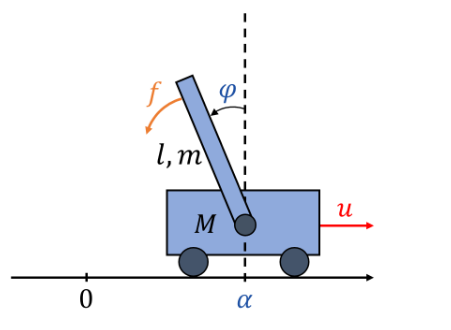
\includegraphics[width=0.8\linewidth]{pic/1_pic_may.png}}
\caption{Перевернутый маятник на тележке.}
\label{1_pic_may}
\end{figure}

Введем переменные состояния

\begin{equation}
    \begin{cases}
        x_1 = a\\
        x_2 = \dot{a}\\
        x_3 = \varphi \\
        x_4 = \dot{ \varphi}
    \end{cases}
\end{equation}

Пусть $T$ -- кинетическая энергия системы, $T_{\text{тележки}}$, $T_{\text{маятника}}$ -- кинетическая энергия тележки и маятника соответственно.

\begin{equation}
    T_{\text{тележки}} = \frac{M \dot{a}^2}{2}
\end{equation}

\begin{equation}
T_{\text{маятника}} = \frac{m}{2} \left( \dot{x}^2_{\text{маятника}} + \dot{y}^2_{\text{маятника}}  \right)  = \frac{\rho Sl}{2} \left( \dot{x}^2_{\text{маятника}} + \dot{y}^2_{\text{маятника}}  \right),
\end{equation}

где $l$ -- длина стержня, $S$ -- площадь сечения, $\rho$ -- плотность.

\begin{multline}
T_{\text{маятника}}   = \frac{\rho Sl}{2} \left( \dot{x}^2_{\text{маятника}} + \dot{y}^2_{\text{маятника}}  \right) = \\=\frac{\rho S}{2} \int \limits_0^l \left( \left( \dot{a} - \left( \lambda\sin \varphi \right)'_t \right)^2 + \left( \left(\lambda \cos \varphi \right)'_t \right)^2 \right) d \lambda =\\=
\frac{m\dot{a}^2}{2} + \frac{\rho S}{2} \int \limits_0^l \left(  -2 \lambda \dot{a} \dot {\varphi} \cos{\varphi} + \lambda^2  \dot {\varphi}^2 \cos^2\varphi +  \lambda^2 \dot{\varphi}^2 \sin^2 \varphi \right) d \lambda =\\= \frac{m\dot{a}^2}{2} + \frac{\rho S}{2} \int \limits_0^l \left(  -2 \lambda \dot{a} \dot {\varphi} \cos{\varphi} + \lambda^2  \dot {\varphi}^2  \right) d \lambda =\\= \frac{m\dot{a}^2}{2} + \frac{\rho S}{2} (-l^2 \dot{a} \dot {\varphi} \cos{\varphi} + \frac{l^3\dot {\varphi}^2}{3})  = 
\frac{m\dot{a}^2}{2} - \frac{ml \dot{a} \dot{\varphi}\cos{\varphi}}{2} + \frac{ml^2\dot {\varphi} ^2}{6}
\end{multline}


\begin{multline}
    T = T_{\text{тележки}} + T_{\text{маятника}} = 
    \frac{M \dot{a}^2}{2} + \frac{m\dot{a}^2}{2} - \frac{ml \dot{a} \dot{\varphi}\cos{\varphi}}{2} + \frac{ml^2\dot {\varphi} ^2}{6} =\\=
    \frac{(M+m) \dot{a}^2}{2} - \frac{ml\dot{a}  \dot{\varphi} \cos \varphi}{2} + \frac{ml^2 \dot{\varphi}^2}{6}
\end{multline}

Запишем систему уравнений Лагранжа

\begin{multline}
    \begin{cases}
        \frac{d}{dt} \frac{\partial T}{\partial \dot{a}} - \frac{\partial T}{\partial a} = u\\
         \frac{d}{dt} \frac{\partial T}{\partial \dot{\varphi}} - \frac{\partial T}{\partial \varphi} = f
    \end{cases} \Rightarrow 
    \begin{cases}
        \left(M+m \right) \ddot{a} - \frac{ml(\ddot{\varphi} \cos \varphi - \dot{\varphi}^2 \sin \varphi)}{2} = u\\
        \frac{ml^2 \ddot{\varphi}}{3} +\frac{ml \dot{a} \dot{\varphi} \sin \varphi}{2} - \frac{ml \ddot{a} \cos \varphi}{2} = f
    \end{cases} \Rightarrow\\ \Rightarrow
     \begin{cases}
        \left(M+m \right) \ddot{a} - \frac{ml(\ddot{\varphi} \cos \varphi - \dot{\varphi}^2 \sin \varphi)}{2} = u\\
        \frac{ml^2 \ddot{\varphi}}{3} -\frac{mgl \sin \varphi}{2} - \frac{ml \ddot{a} \cos \varphi}{2} = f
    \end{cases}
\end{multline}

Преобразуем данную систему уравнений

\begin{equation}
\begin{cases}
    \ddot{a} = - \frac{3 \cos{\varphi} \sin {\varphi} g lm + 6 \cos{\varphi}f-2 \dot{\varphi}^2\sin{\varphi}l^2m+4lu}{l(3 \cos^2 \varphi m - 4m -4M)}\\[2ex]
    \ddot{\varphi} = \frac{3(\cos \varphi \sin \varphi \dot{\varphi}^2l^2m^2-2lmu \cos{\varphi}-2glm^2 \sin{\varphi} - 2 glmM \sin{\varphi} - 4fm - 4fM)}{l^2m(3m \cos^2 \varphi -4m-4M)}
    \end{cases}
\end{equation}


\begin{equation}
\label{1_model_full}
    \begin{cases}
        \dot{x}_1 = x_2\\
        \dot{x}_2 = - \frac{3 \cos{\varphi} \sin {\varphi} g lm + 6 \cos{\varphi}f-2 \dot{\varphi}^2\sin{\varphi}l^2m+4lu}{l(3 \cos^2 \varphi m - 4m -4M)}\\
        \dot{x}_3 = x_4\\
        \dot{x}_4  = \frac{3(\cos \varphi \sin \varphi \dot{\varphi}^2l^2m^2-2lmu \cos{\varphi}-2glm^2 \sin{\varphi} - 2 glmM \sin{\varphi} - 4fm - 4fM)}{l^2m(3m \cos^2 \varphi -4m-4M)}\\
        y_1 = x_1\\
        y_2 = x_3
    \end{cases}
\end{equation}


\section{Точки равновесия}
Найдем точки равновесия системы из условия $\dot{x}_i = 0$ и $u=0$, $f = 0$

\begin{multline}
    \begin{cases}
        \dot{x}_1 = x_2 = 0\\
        \dot{x}_2 = - \frac{3 \cos{\varphi} \sin {\varphi} g lm + 0-2 \dot{\varphi}^2\sin{\varphi}l^2m+0}{l(3 \cos^2 \varphi m - 4m -4M)} = 0\\
        \dot{x}_3 = x_4 = 0\\
        \dot{x}_4  = \frac{3(\cos \varphi \sin \varphi \dot{\varphi}^2l^2m^2-0-2glm^2 \sin{\varphi} - 2 glmM \sin{\varphi} - 0 - 0)}{l^2m(3m \cos^2 \varphi -4m-4M)} = 0\\
    \end{cases} \Rightarrow \\ \Rightarrow
    \begin{cases}
        \dot{x}_1 = x_2 = \dot{a} =0\\
        \dot{x}_2 = - \frac{3 \cos{\varphi} \sin {\varphi} g lm -2 \dot{\varphi}^2\sin{\varphi}l^2m}{l(3 \cos^2 \varphi m - 4m -4M)} = 0\\
        \dot{x}_3 = x_4 = \dot{\varphi} = 0\\
        \dot{x}_4  = \frac{3(\cos \varphi \sin \varphi \dot{\varphi}^2l^2m^2-2glm^2 \sin{\varphi} - 2 glmM \sin{\varphi} )}{l^2m(3m \cos^2 \varphi -4m-4M)} = 0\\
    \end{cases} \Rightarrow \\ \Rightarrow
    \begin{cases}
        \dot{x}_2 = - \frac{3 \cos{\varphi} \sin {\varphi} g lm}{l(3 \cos^2 \varphi m - 4m -4M)} = 0\\
        \dot{x}_4  = \frac{3(-2glm^2 \sin{\varphi} - 2 glmM \sin{\varphi} )}{l^2m(3m \cos^2 \varphi -4m-4M)} = 0\\
    \end{cases} \Rightarrow
    \begin{cases}
        \cos{\varphi} \sin{\varphi} = 0\\
        m\sin{\varphi}+M \sin{\varphi} = 0
    \end{cases} \Rightarrow \\
    \Rightarrow
    \varphi = \pi k, k \in \mathbf{Z}
\end{multline}

Запишем вектор состояния для точек равновесия

\begin{equation}
    \begin{cases}
        x_1 = a \in \mathbf{R}\\
        x_2 = \dot{a} = 0\\
        x_3 = \varphi = \pi k, k \in \mathbf{Z} \\
        x_4 = \dot{\varphi} = 0
    \end{cases}
\end{equation}

\section{Линеаризация}

Линеаризуем уравнение объекта около точки равновесия $(x,u,f) = 0$ (в нашем случае -- верхнее положение маятника). При линеаризации воспользуемся следующими приемами: $\sin x \approx x$, $\cos x \approx 1$, $x^{n+1} \approx 0$ для малых $x$ и $n \in \mathbf{N}$. Будем считать $\varphi$ малым.

\begin{multline}
    \begin{cases}
        \dot{x}_1 = x_2\\
        \dot{x}_2 = - \frac{3 \cos{\varphi} \sin {\varphi} g lm + 6 \cos{\varphi}f-2 \dot{\varphi}^2\sin{\varphi}l^2m+4lu}{l(3 \cos^2 \varphi m - 4m -4M)}\\
        \dot{x}_3 = x_4\\
        \dot{x}_4  = \frac{3(\cos \varphi \sin \varphi \dot{\varphi}^2l^2m^2-2lmu \cos{\varphi}-2glm^2 \sin{\varphi} - 2 glmM \sin{\varphi} - 4fm - 4fM)}{l^2m(3m \cos^2 \varphi -4m-4M)}
    \end{cases} \Rightarrow\\
    \Rightarrow
    \begin{cases}
        \dot{x}_1 = x_2\\
        \dot{x}_2 =  \frac{3  x_3 g lm + 6 f+4lu}{l(m +4M)}\\
        \dot{x}_3 = x_4\\
        \dot{x}_4  = \frac{3( 2lmu +2glm^2 x_3 + 2 glmM x_3 + 4fm + 4fM)}{l^2m(m+4M)}
    \end{cases}  \Rightarrow\\
    \Rightarrow
    \begin{cases}
        \dot{x}_1 = x_2\\
        \dot{x}_2 =  \frac{3   g m}{m +4M}x_3 + \frac{4}{m +4M}u + \frac{6 }{l(m +4M)}f\\
        \dot{x}_3 = x_4\\
        \dot{x}_4  = \frac{6g( m  +  M  )}{l(m+4M)}x_3 + \frac{6  }{l(m+4M)}u + \frac{12(  m + M)}{l^2m(m+4M)}f
    \end{cases} 
\end{multline}

Перейдем к математической модели в виде
\begin{equation}
\label{1_model_lin}
\begin{cases}
     \dot{x} = Ax + Bu + Df,\\
     y=Cx,
\end{cases}
\end{equation}
где $A$, $B$, $C$, $D$ -- постоянные матрицы, зависящие от значений $M$, $m$, $g$, $l$. Здесь $x = (x_1, \dots , x_4)$ -- совокупный вектор состояния, $y = (y_1,  y_2)$ -- вектор измеряемых величин.

\begin{multline}
    A = \begin{bmatrix}
        0 & 1 & 0 & 0\\
        0 & 0 &  \frac{3   g m}{m +4M} & 0\\
        0 & 0 & 0 & 1\\
        0 & 0 & \frac{6g( m  +  M  )}{l(m+4M)} & 0
    \end{bmatrix}, 
    B = \begin{bmatrix}
        0\\
        \frac{4}{m +4M}\\
        0\\
        \frac{6  }{l(m+4M)}
    \end{bmatrix},\\ 
    C^T = \begin{bmatrix}
        1 & 0\\
        0 & 0\\
        0 & 1\\
        0 & 0
    \end{bmatrix}, 
    D = \begin{bmatrix}
        0\\
        \frac{6 }{l(m +4M)}\\
        0\\
        \frac{12(  m + M)}{l^2m(m+4M)}
    \end{bmatrix}
\end{multline}

\section{Выбор исходных данных}

Получим численные значения массы тележки $M=264.5866$, массы маятника $m = 9.1747$ и длины маятника $l =2.5849$. Ускорение свободного падения $g = 9.81 \, \,  \frac{\text{м}}{\text{с}^2}$.

После подстановки численных значений получим следующие матрицы системы

\begin{multline}
    A = \begin{bmatrix}
        0 & 1 & 0 & 0\\
        0 & 0 &  0.2529 & 0\\
        0 & 0 & 0 & 1\\
        0 & 0 & 5.8395 & 0
    \end{bmatrix}, 
    B = \begin{bmatrix}
        0\\
        0.0037\\
        0\\
        0.0022
    \end{bmatrix},\\ 
    C^T = \begin{bmatrix}
        1 & 0\\
        0 & 0\\
        0 & 1\\
        0 & 0
    \end{bmatrix}, 
    D = \begin{bmatrix}
        0\\
        0.0022\\
        0\\
        0.0502
    \end{bmatrix}
\end{multline}


\endinput                                     % Первая глава
\chapter{Анализ математической модели}
\label{ch:chap2}

\section{Анализ матриц}
Найдем собственные числа и собственные вектора матрицы $A$ модели (\ref{1_model_lin}).

\begin{equation}
    \begin{cases}
        \lambda_1 = 0 & v_1 = \begin{bmatrix}
            1 & 0 & 0 & 0
        \end{bmatrix}^T\\
         \lambda_2 = 0&  v_2 = \begin{bmatrix}
            -1 & 0 & 0 & 0
        \end{bmatrix}^T\\
         \lambda_3 = 2.4165 & v_3 = \begin{bmatrix}
            0.0165 & 0.0400 & 0.3820 & 0.9231
        \end{bmatrix}^T\\
         \lambda_4 = -2.4165 & v_4 = \begin{bmatrix}
            -0.0165 & 0.0400 & -0.3820 & 0.9231
        \end{bmatrix}^T
    \end{cases}
\end{equation}

Заметим, что в спектр матрицы $A$ входит число с положительной вещественной частью, следовательно, система $\ref{1_model_full}$ неустойчива.

\subsection{Управляемость и стабилизируемость системы}
Составим матрицу управляемости и определим ее ранг

\begin{multline}
    U = \begin{bmatrix}
        B & AB & A^2B&A^3B
    \end{bmatrix} = \begin{bmatrix}
        0 &   0.0037  &       0  &  0.0005\\
    0.0037      &   0   & 0.0005   &      0\\
         0   & 0.0022   &      0  &  0.0127\\
    0.0022     &    0 &   0.0127   &      0
    \end{bmatrix} \Rightarrow\\
    \Rightarrow rank(U) = 4
\end{multline}
Ранг матрицы управляемости равен размерности системы, следовательно, система является полностью управляемой, а значит и стабилизируемой.


\subsection{Наблюдаемость и обнаруживаемость системы}

Составим матрицу наблюдаемости и определим ее ранг

\begin{equation}
    V = \begin{bmatrix}
        C \\ CA \\ CA^2\\ CA^3
    \end{bmatrix} = \begin{bmatrix}
           1&         0     &    0    &     0\\
         0   &      0 &   1  &      0\\
         0 &   1 &         0 &        0\\
         0     &    0&         0 &   1\\
         0    &     0 &    0.2529     &    0\\
         0     &    0 &   5.8395    &     0\\
         0     &    0    &     0  &  0.2529\\
         0     &    0    &     0   & 5.8395
    \end{bmatrix} 
    \Rightarrow rank(V) = 4
\end{equation}
Ранг матрицы наблюдаемости равен размерности системы, следовательно, система является полностью наблюдаемой, а значит и обнаруживаемой.

\section{Передаточные матрицы}

Найдем передаточную матрицу $W_{u \to y}(s)$

\begin{equation}
    W_{u \to y} (s) = C \left(sI-A  \right)^{-1}B = \begin{bmatrix}
        \frac{0.003747s^2 -0.02133}{s^4-5.839s^2}\\[2ex]
        \frac{0.002174}{s^2-5.839}
    \end{bmatrix}
\end{equation}

Динамический порядок $ \frac{0.003747s^2 -0.02133}{s^4-5.839s^2}$ равен 4, относительный динамический порядок 2; динамический порядок $\frac{0.002174}{s^2-5.839}$ равен 2, относительный динамический порядок равен 2.

Нули функции $\frac{0.003747s^2 -0.02133}{s^4-5.839s^2}$ равны $s_0 =\pm 2.3859$, полюса $s_p = \{ 0; 0; \pm 2.4165 \}$.

Полюса $\frac{0.002174}{s^2-5.839}$ равны $s_p = \{ \pm 2.4165 \}$.

Найдем передаточную матрицу $W_{f \to y}(s)$

\begin{equation}
    W_{f \to y} (s) = C \left(sI-A  \right)^{-1}D = \begin{bmatrix}
        \frac{0.002174}{s^2-5.839}\\[2ex]
        \frac{0.0502}{s^2-5.839}
    \end{bmatrix}
\end{equation}

Динамический порядок $ \frac{0.002174}{s^2-5.839}$ равен 2, относительный динамический порядок 2; динамический порядок $\frac{0.0502}{s^2-5.839}$ равен 2, относительный динамический порядок равен 2.

Полюса для  $ \frac{0.002174}{s^2-5.839}$ и $\frac{0.0502}{s^2-5.839}$ одинаковы и равны $s_p = \{ \pm 2.4165 \}$.

Заметим, что полюса всех передаточных функций содержат в себе собственные числа матрицы $A$ $\lambda_{3,4}$ -- для функций, кроме первой, полюса первой передаточной функции совпадают с собственными числами матрицы $A$.

С физической точки зрения, все передаточные функции описывают расходящийся переходный процесс при $u=0$ и $f=0$.


\section{Моделирование}

Зададим начальные условия $$x_{0_1} = \begin{bmatrix}
     0.01\\
    0.01\\
    0.01\\
    0.05
\end{bmatrix},  x_{0_2} = \begin{bmatrix}
    0.01\\
    0.01\\
    0.05\\
    0.01
\end{bmatrix},  x_{0_3} = \begin{bmatrix}
    0.01\\
    0.05\\
    0.01\\
    0.01
\end{bmatrix}$$
и выполним моделирование линеаризованного (\ref{1_model_lin}) и нелинеаризованного объекта (\ref{1_model_full}) на малом и большем отрезке времени: 1 и 10 секунд, соответственно.


\begin{figure}[!h]
\center{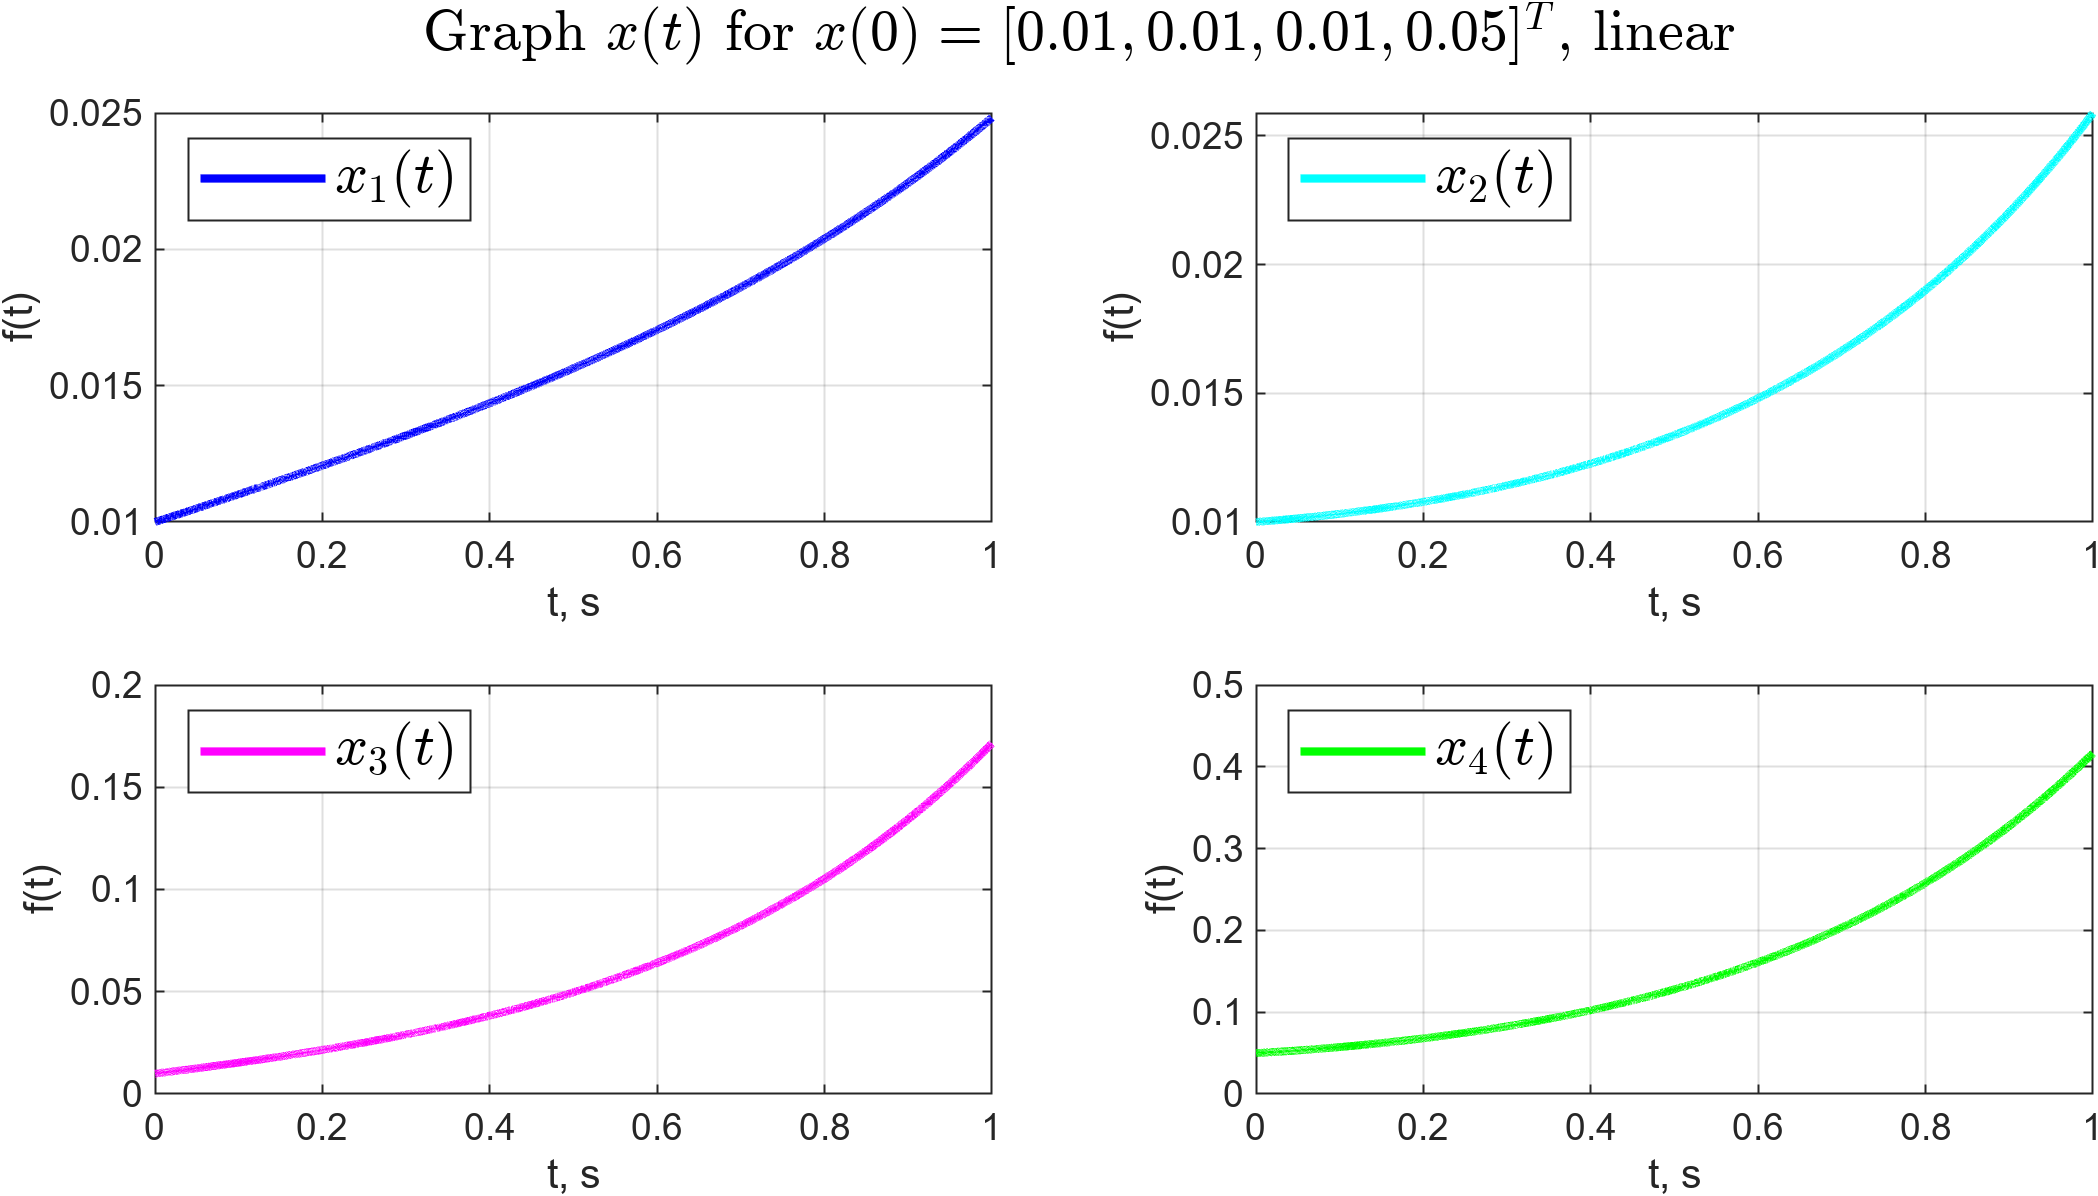
\includegraphics[width=1\linewidth]{pic/2_x_lin_04_sm.png}}
\caption{График вектора состояния линеаризованной системы, время моделирования $t=1$ с, начальные условия $x_{0_1}$.}
\label{2_x_lin_01_sm}
\end{figure}

\begin{figure}[!h]
\center{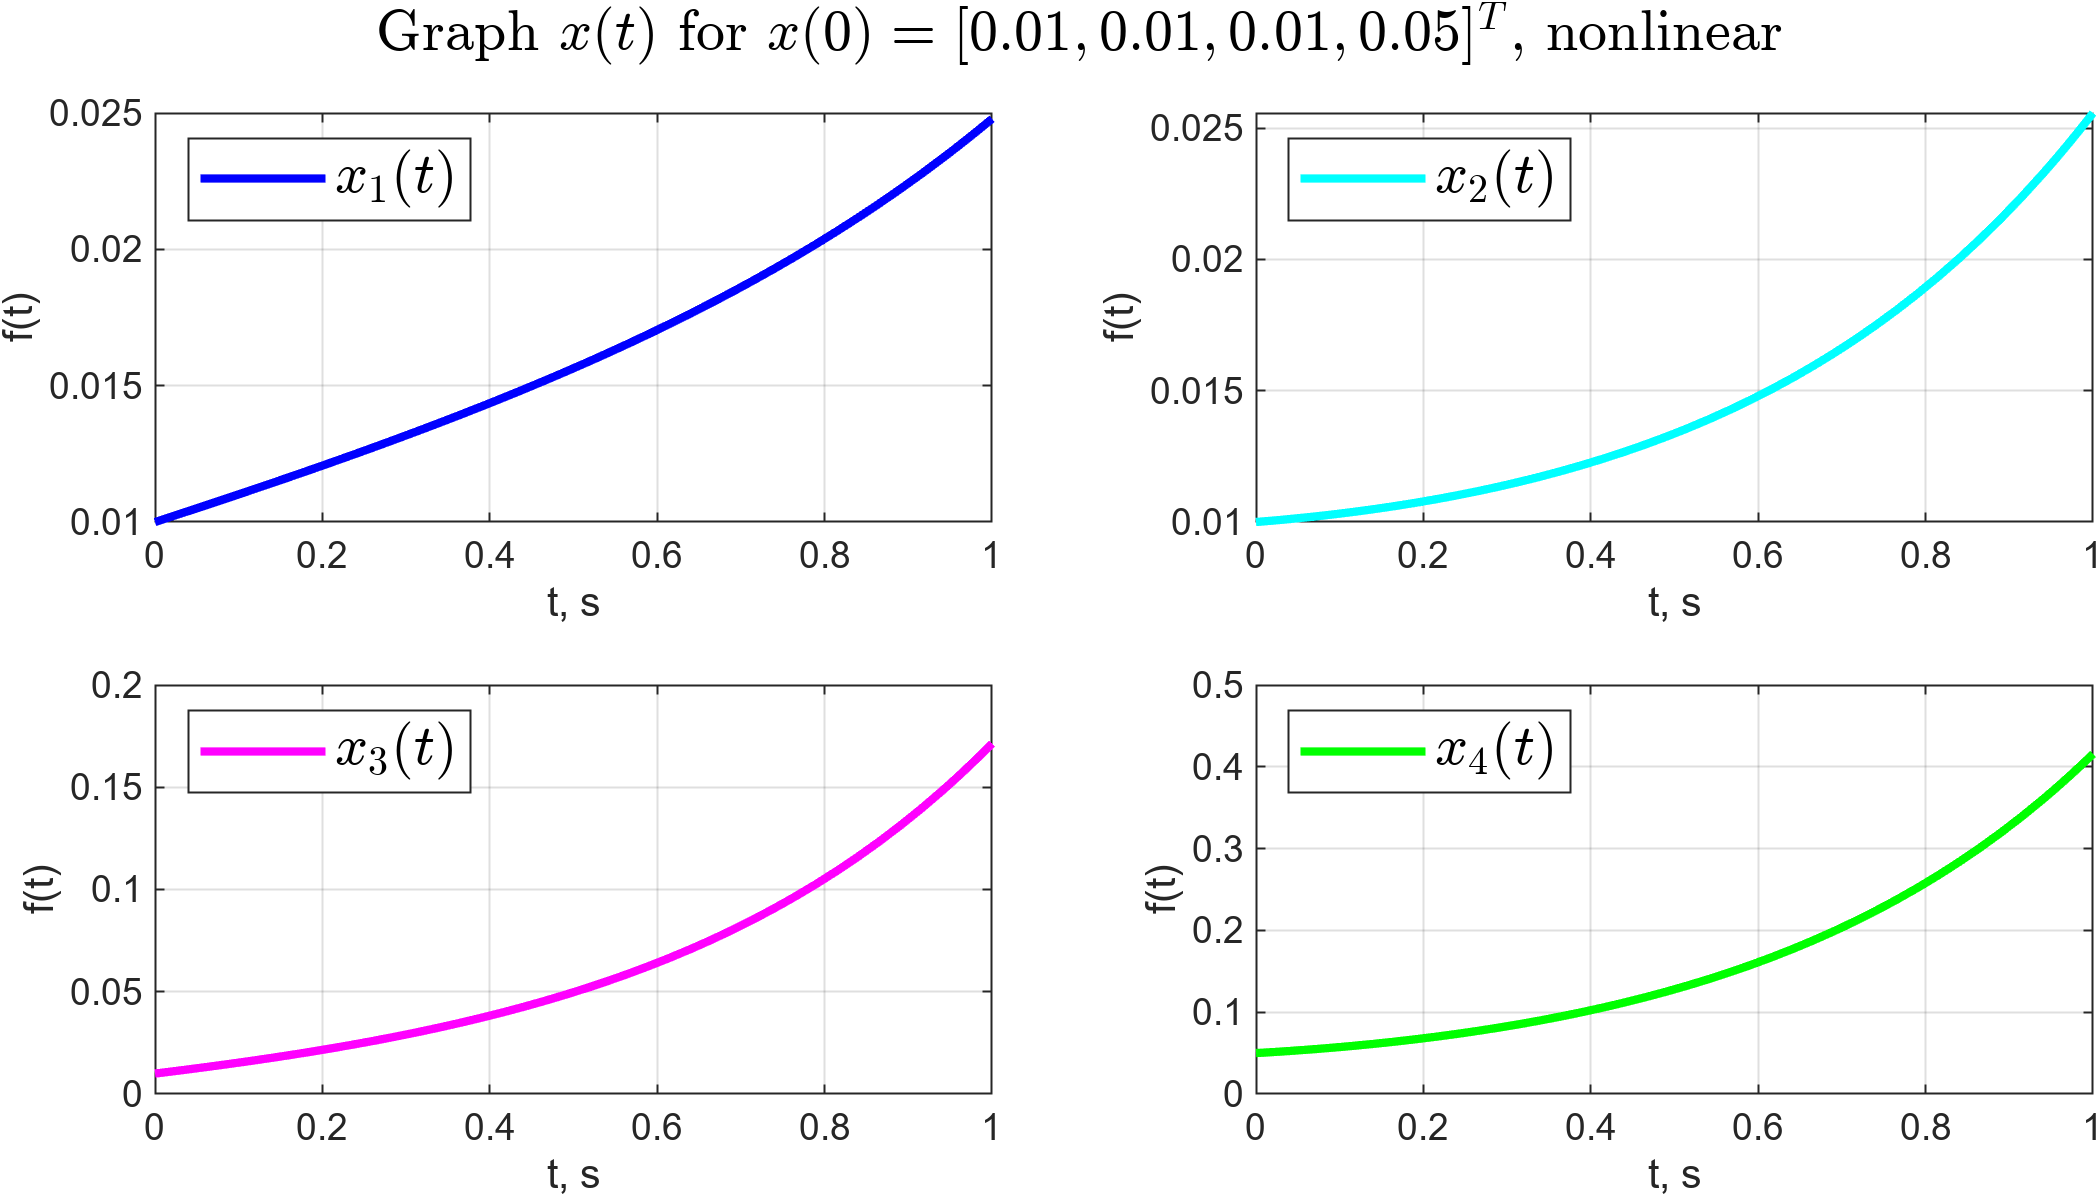
\includegraphics[width=1\linewidth]{pic/2_x_nlin_04_sm.png}}
\caption{График вектора состояния исходной системы, время моделирования $t=1$ с, начальные условия $x_{0_1}$.}
\label{2_x_nlin_01_sm}
\end{figure}

\begin{figure}[!h]
\center{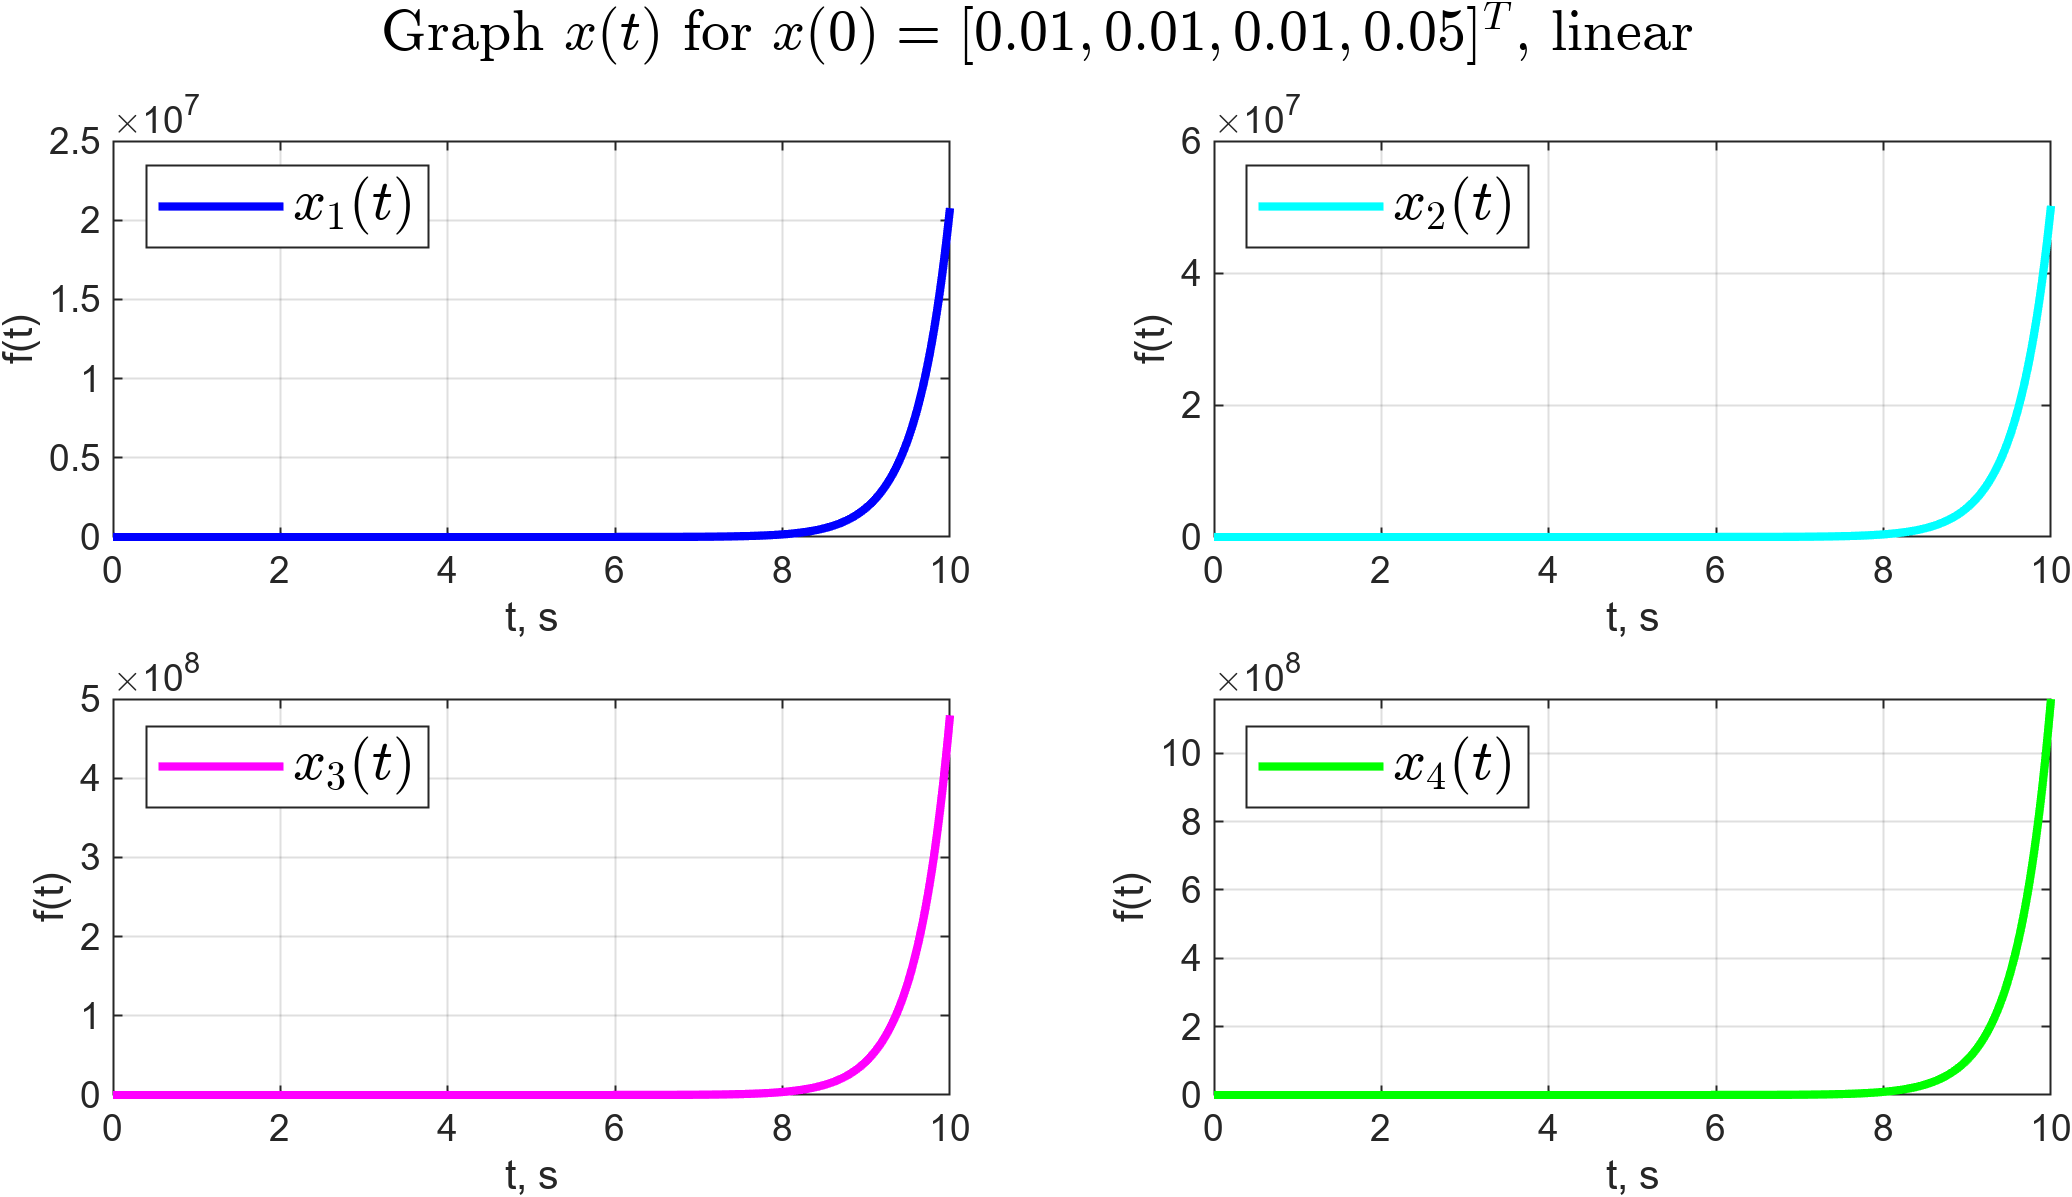
\includegraphics[width=1\linewidth]{pic/2_x_lin_04_lg.png}}
\caption{График вектора состояния линеаризованной системы, время моделирования $t=10$ с, начальные условия $x_{0_1}$.}
\label{2_x_lin_01_lg}
\end{figure}

\begin{figure}[!h]
\center{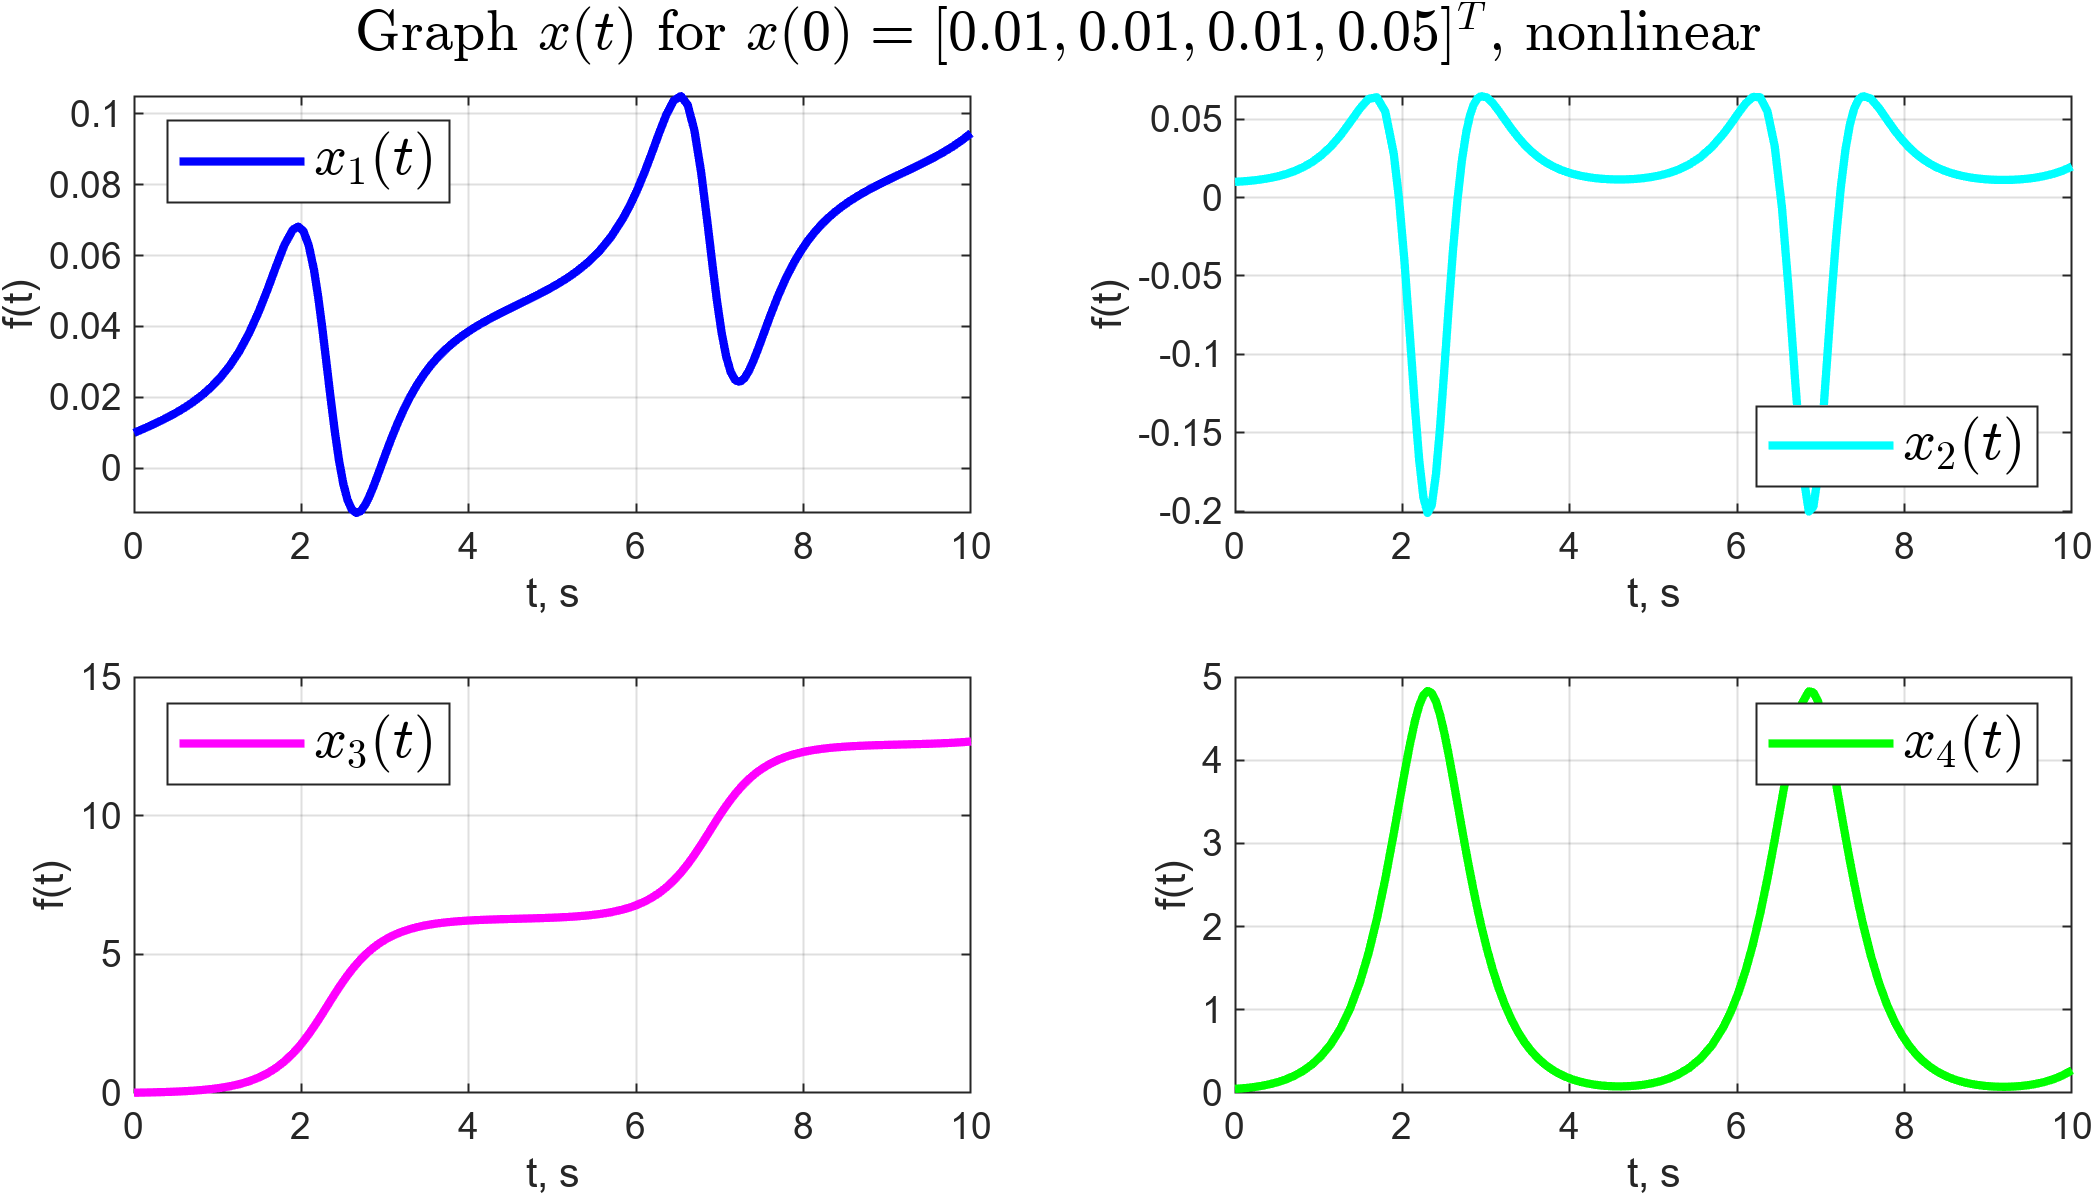
\includegraphics[width=1\linewidth]{pic/2_x_nlin_04_lg.png}}
\caption{График вектора состояния исходной системы, время моделирования $t=10$ с, начальные условия $x_{0_1}$.}
\label{2_x_nlin_01_lg}
\end{figure}

Заметим, что для малого времени моделирования ($t=1$ с) графики состояния линеаризованной и нелинеаризованной систем близки между собой, однако в случае увеличения времени моделирования до $t=10$ с, поведение линеаризованной модели сильно отличается от исходной. Это происходит потому, что в ходе линеаризации мы считали углы отклонения маятника от вертикали малыми. 

Поведение, которое мы наблюдаем для нелинеаризованной модели (рисунок \ref{2_x_nlin_01_lg}) близко к поведению реального физического объекта: координата тележки $x_1$ совершает колебания (то есть движется из стороны в сторону) с постепенным смещением вверх, график угла отклонения $x_3$ совершает переходы от $\pi k$ к $\pi(k+1), k \in \mathbf{Z}$ (то есть совершает обороты около точки крепления), кроме того, мы видим, что энергия системы сохраняется: максимальная по модулю угловая скорость маятника достигается в нижней точке, минимальная -- в верхней.


Далее выполним моделирование систем с начальными условиями $x_{0_2}$, то есть зададим  большее значение угла отклонения маятника от вертикали.
\begin{figure}[!h]
\center{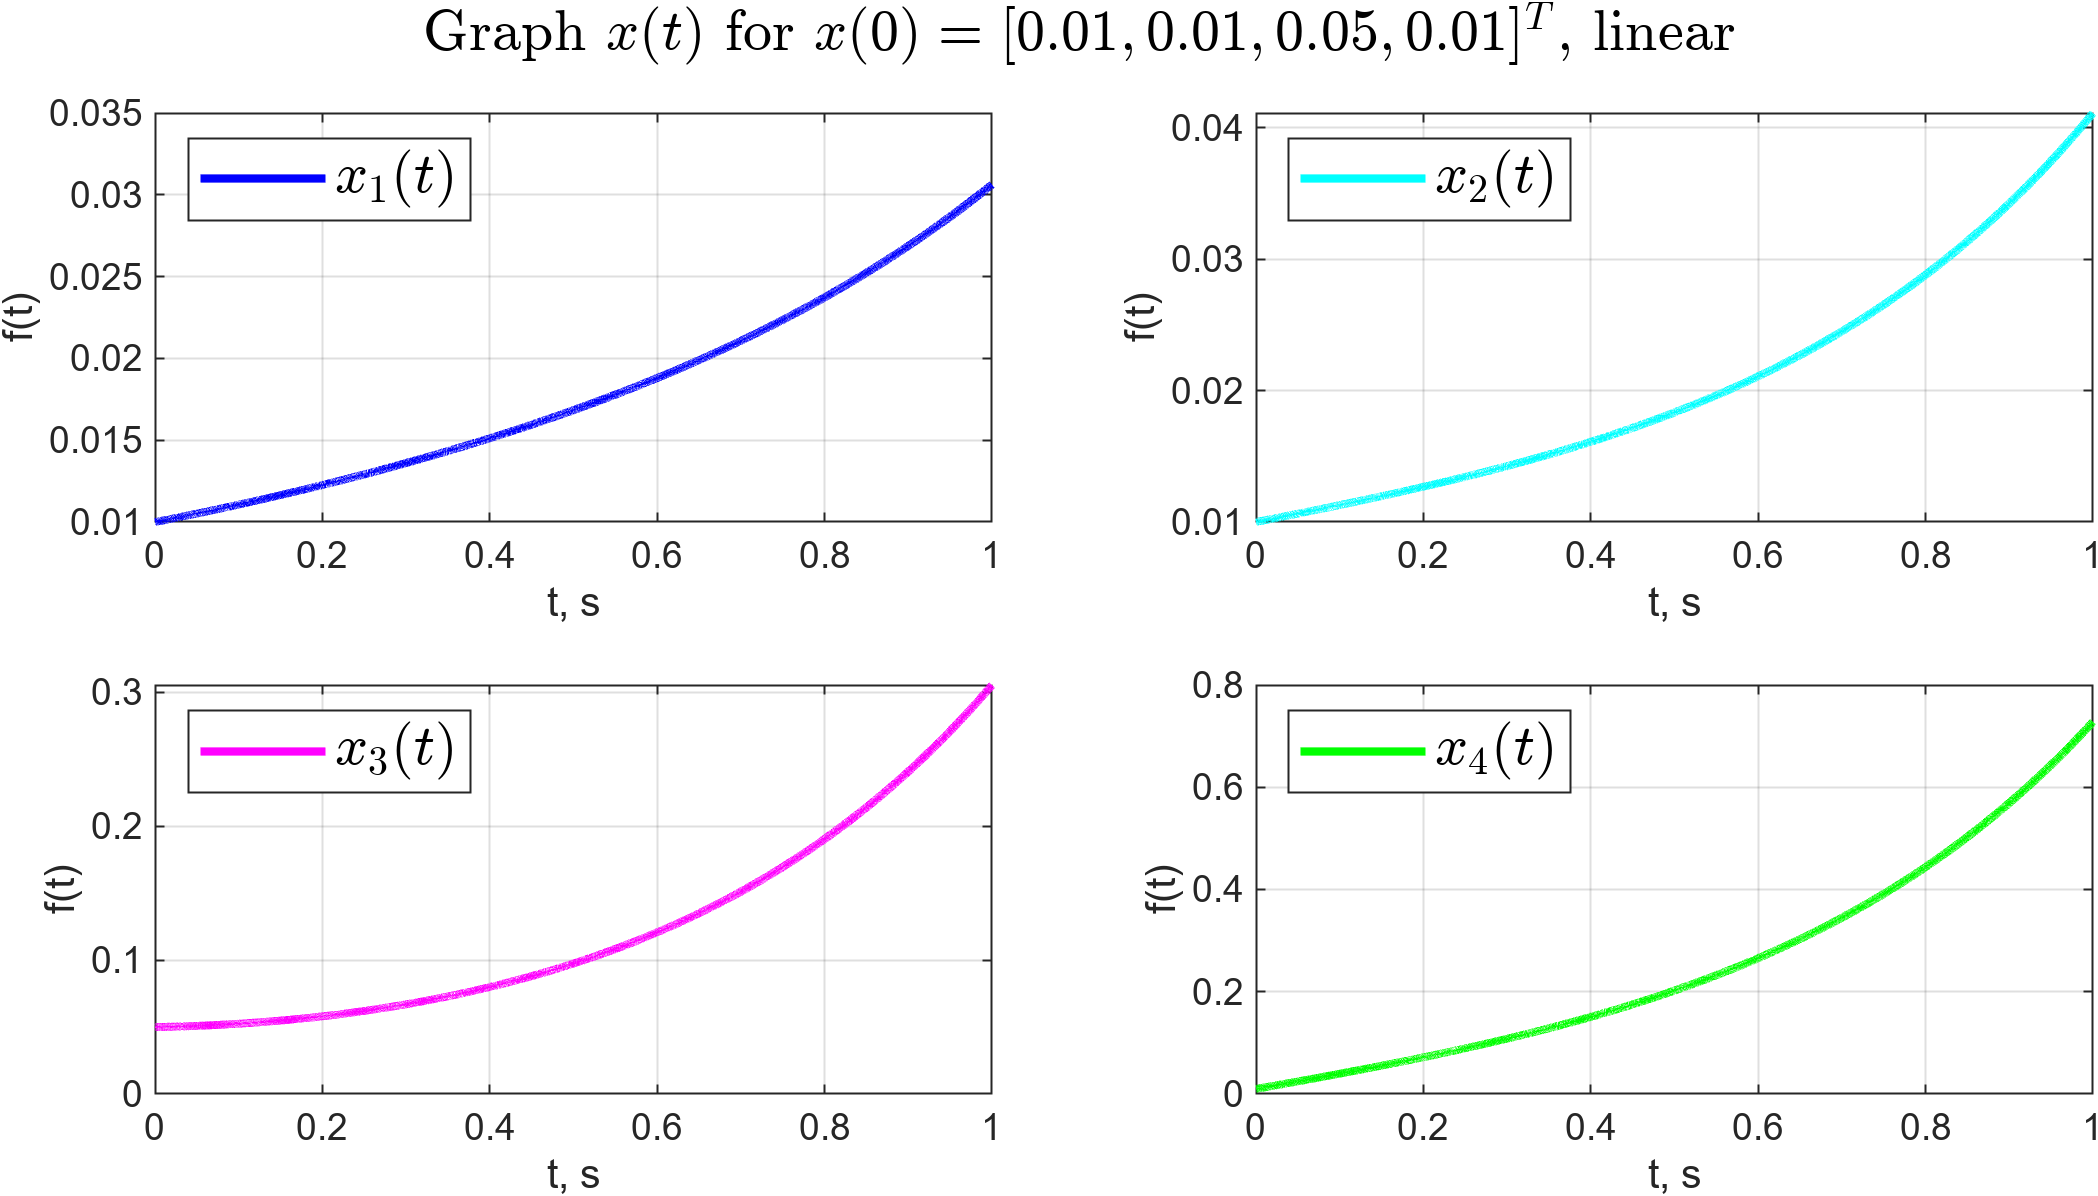
\includegraphics[width=1\linewidth]{pic/2_x_lin_02_sm.png}}
\caption{График вектора состояния линеаризованной системы, время моделирования $t=1$ с, начальные условия $x_{0_2}$.}
\label{2_x_lin_02_sm}
\end{figure}

\begin{figure}[!h]
\center{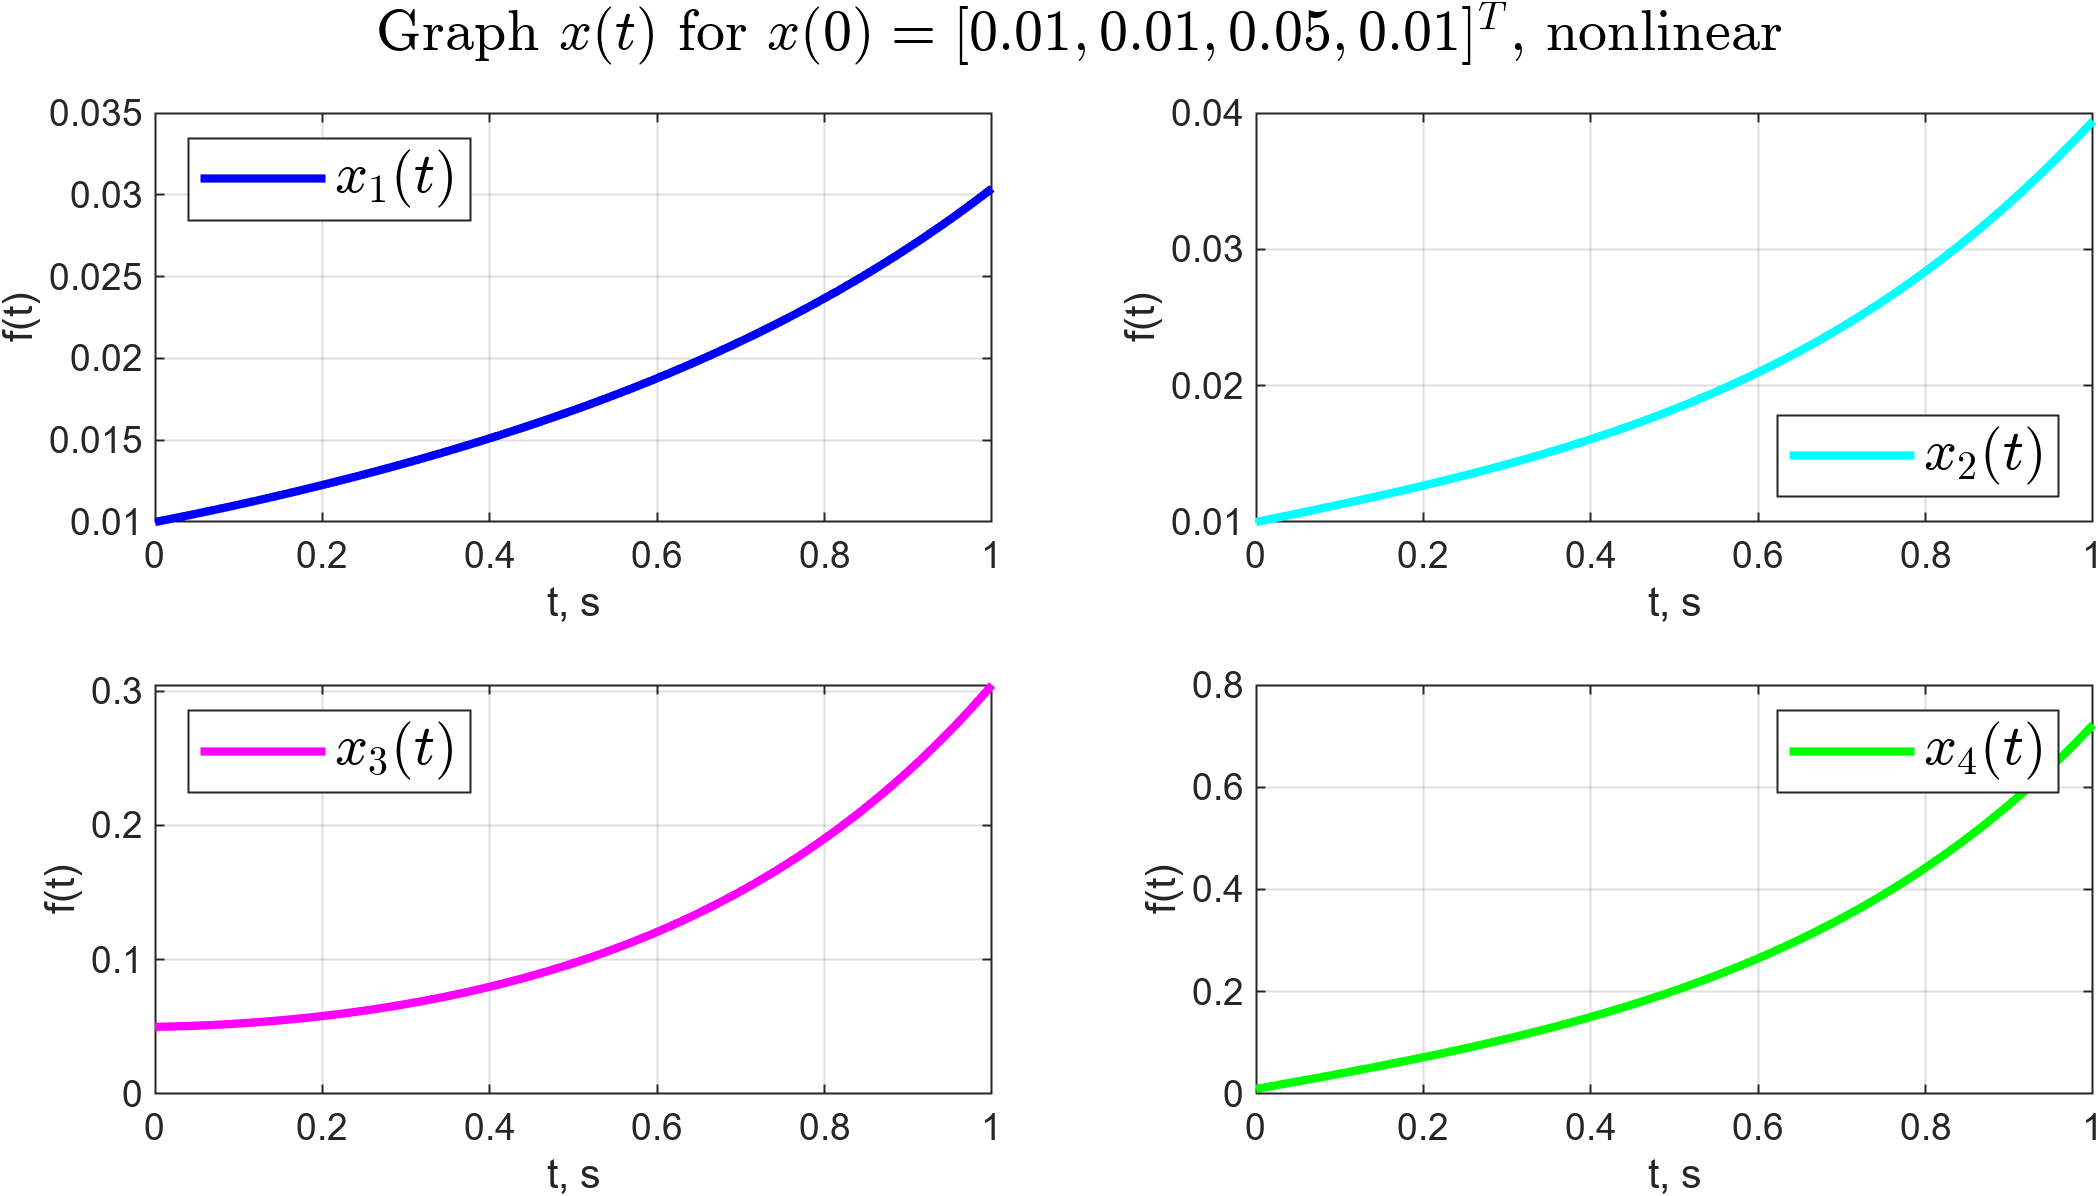
\includegraphics[width=1\linewidth]{pic/2_x_nlin_02_sm.png}}
\caption{График вектора состояния исходной системы, время моделирования $t=1$ с, начальные условия $x_{0_2}$.}
\label{2_x_nlin_02_sm}
\end{figure}

\begin{figure}[!h]
\center{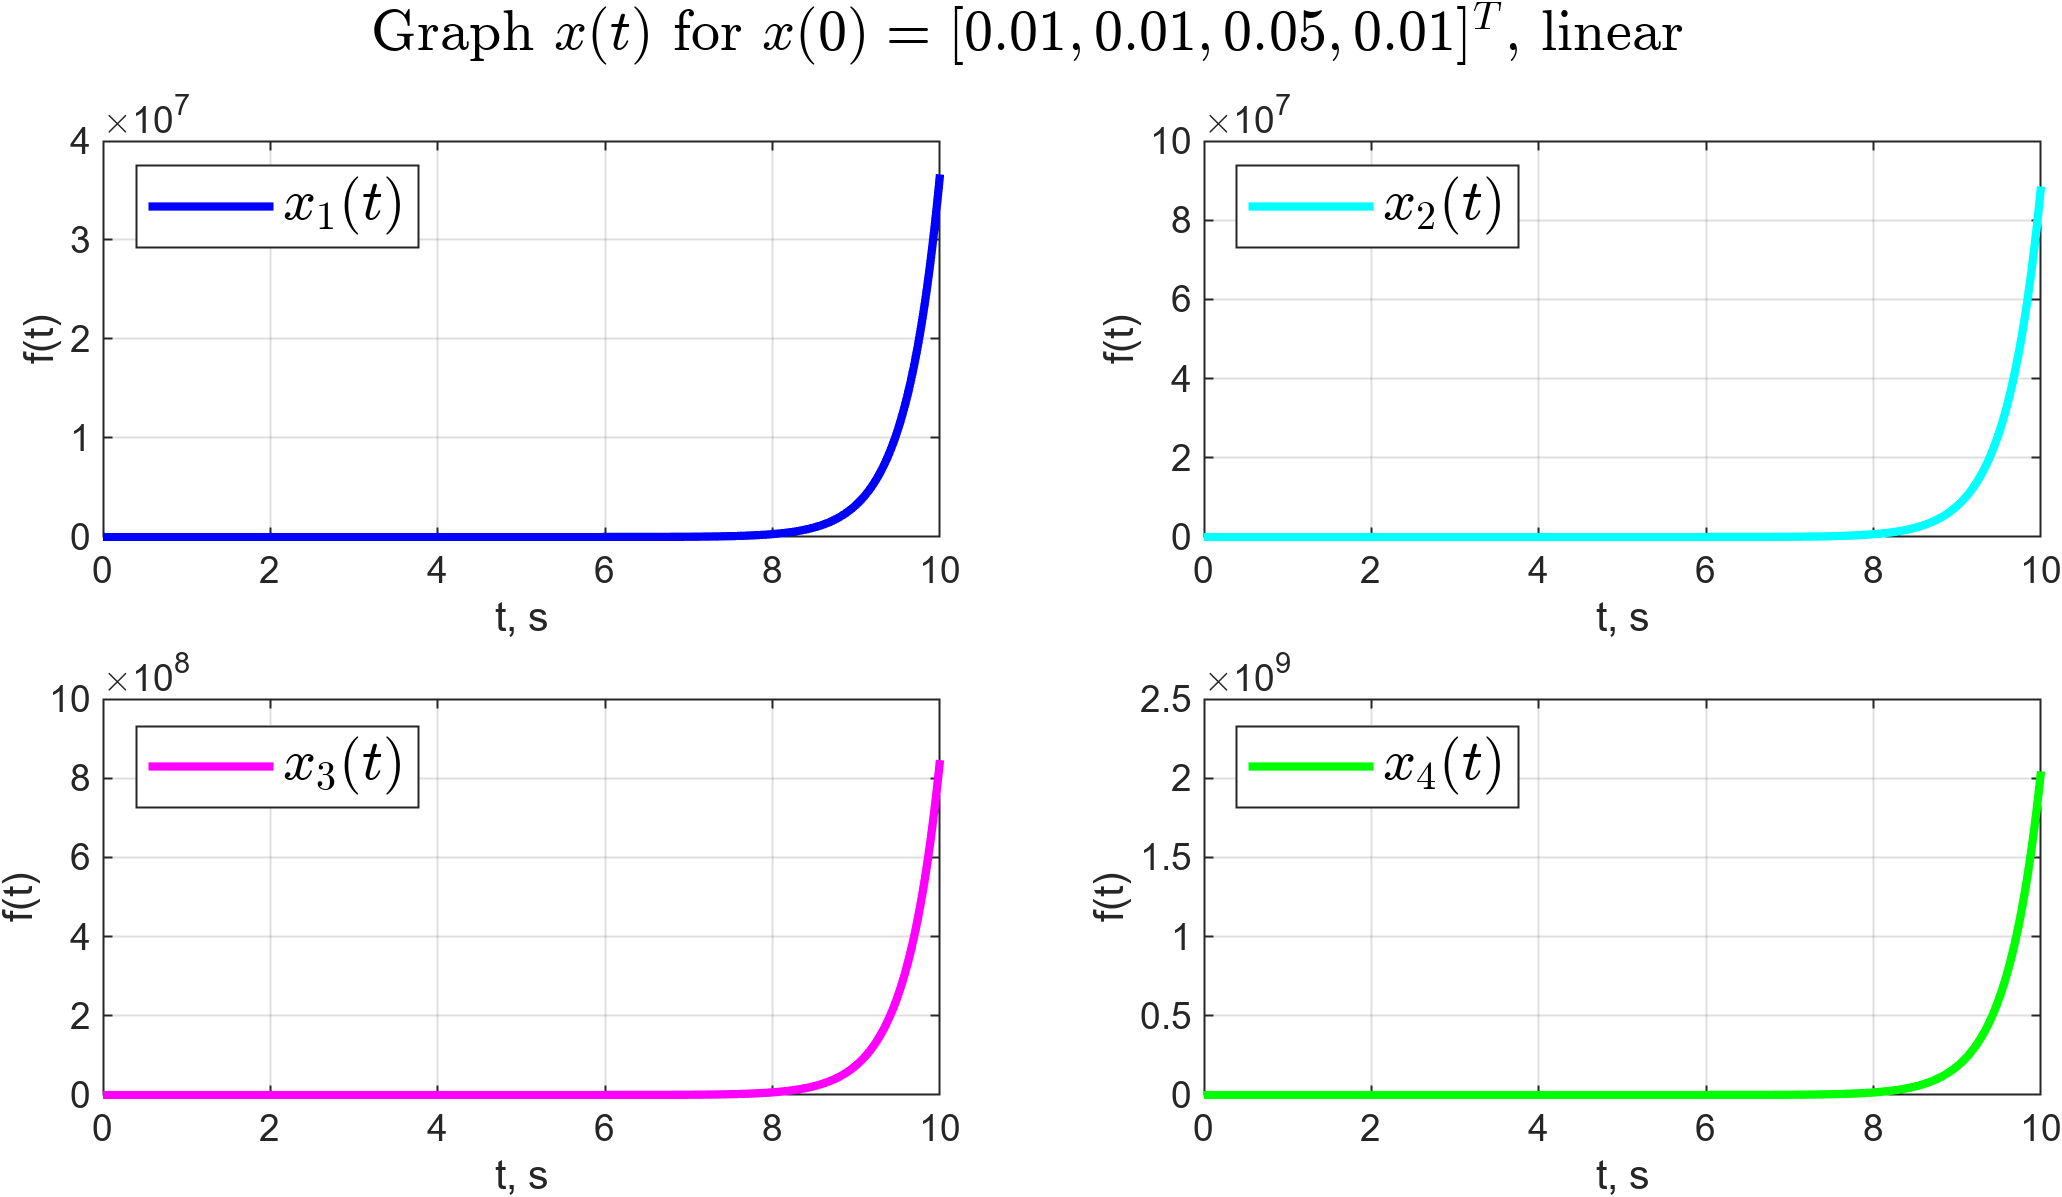
\includegraphics[width=1\linewidth]{pic/2_x_lin_02_lg.png}}
\caption{График вектора состояния линеаризованной системы, время моделирования $t=10$ с, начальные условия $x_{0_2}$.}
\label{2_x_lin_02_lg}
\end{figure}

\begin{figure}[!h]
\center{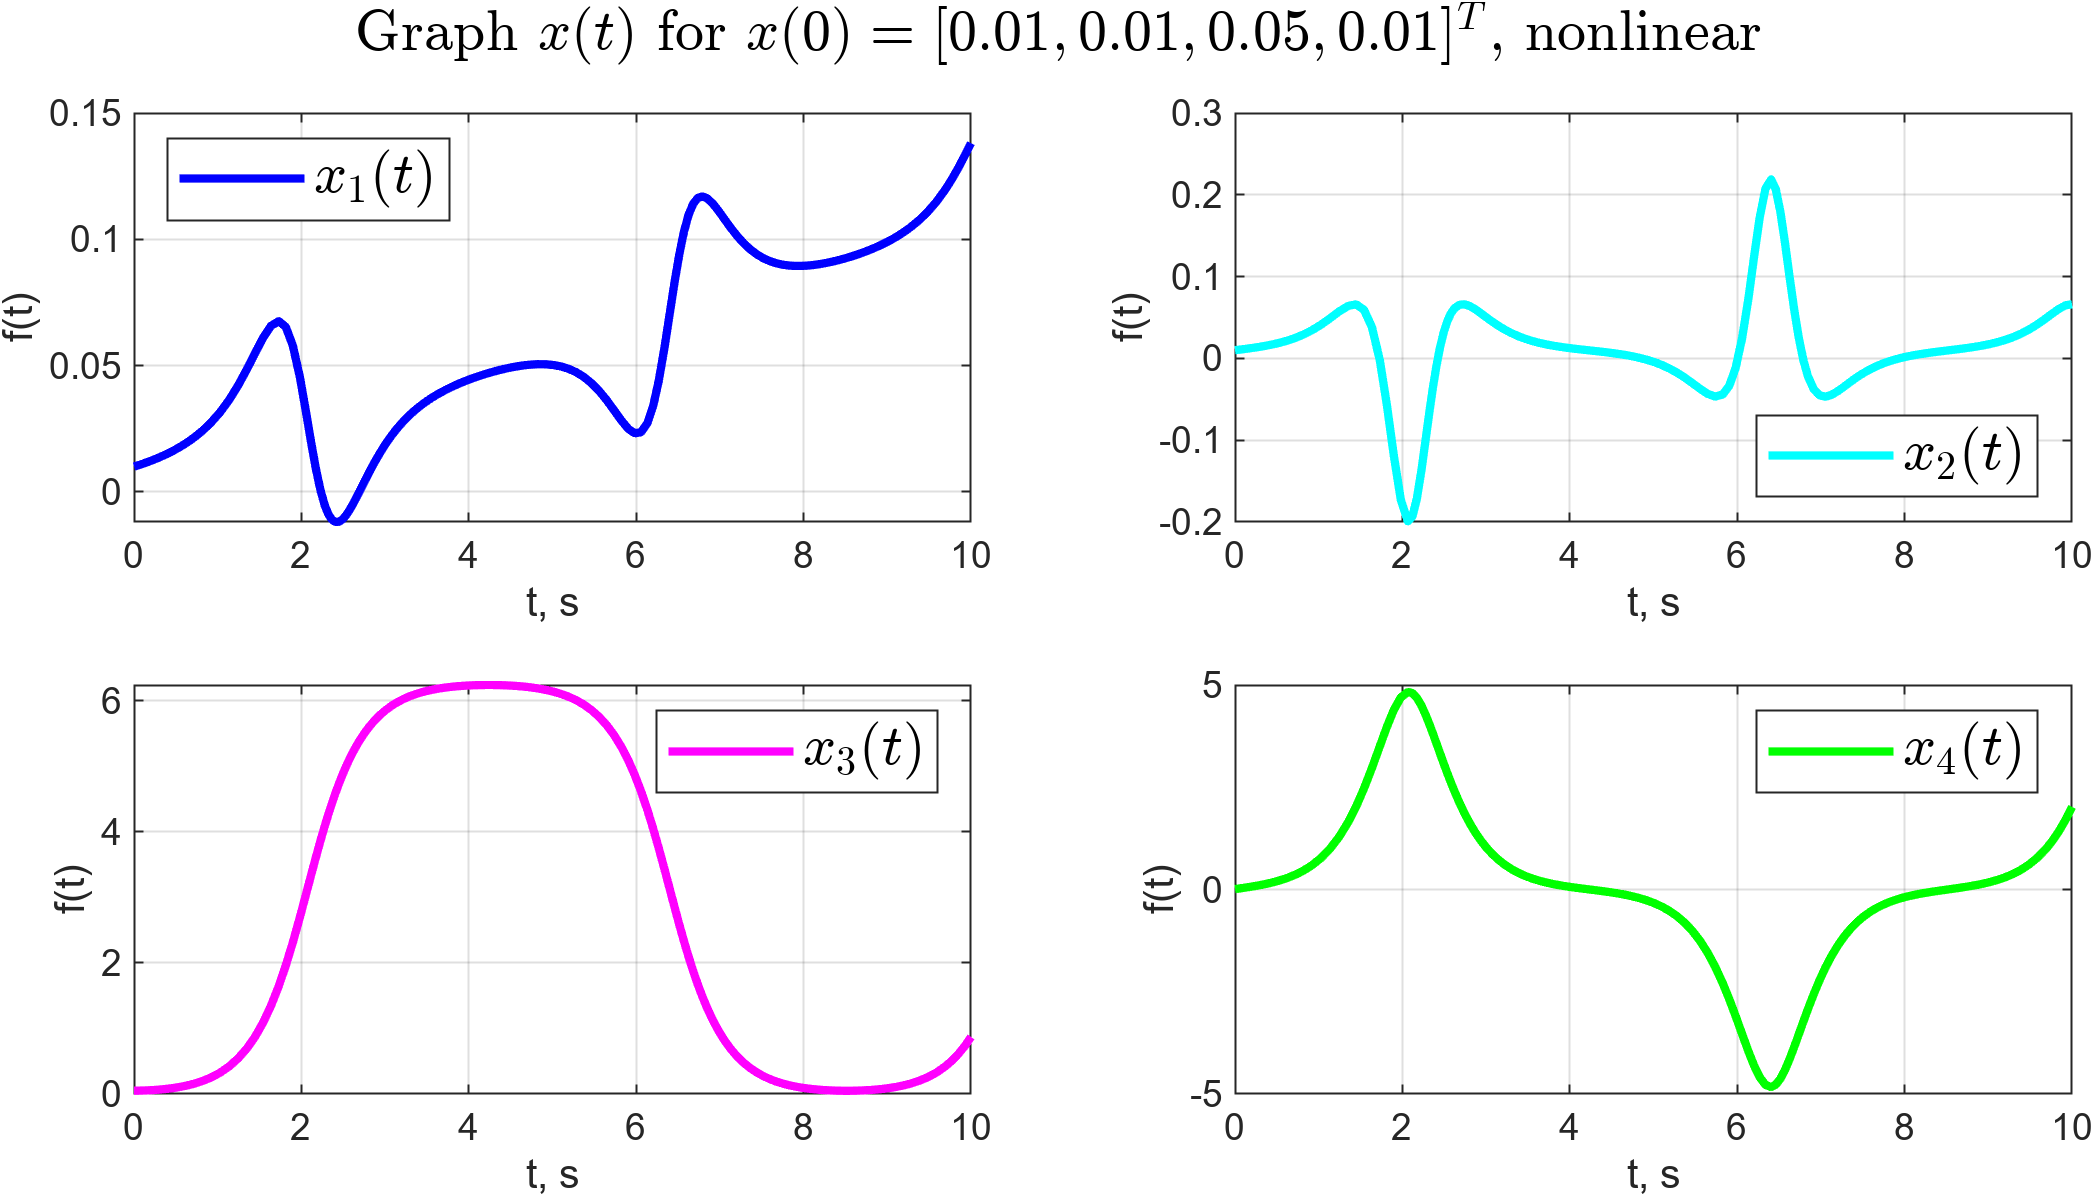
\includegraphics[width=1\linewidth]{pic/2_x_nlin_02_lg.png}}
\caption{График вектора состояния исходной системы, время моделирования $t=10$ с, начальные условия $x_{0_2}$.}
\label{2_x_nlin_02_lg}
\end{figure}




\newpage
\,
\newpage



Заметим, что поведение линеаризованной и исходной системы вновь схожи при малом времени моделирования $t=1$ c (рисунки \ref{2_x_lin_02_sm} и \ref{2_x_nlin_02_sm}). При увеличении времени моделирования до $t=10$ с линеаризованная система вновь сильно отличается от исходной. Кроме того, теперь маятник совершает колебания от $\varphi \approx 0$ до $\varphi \approx 2 \pi$. 




Далее рассмотрим поведение системы при начальных условиях $x_{0_3}$ -- здесь значения также близки к нулю, но теперь больше начальная скорость тележки $x_2(0)$.

\begin{figure}[!h]
\center{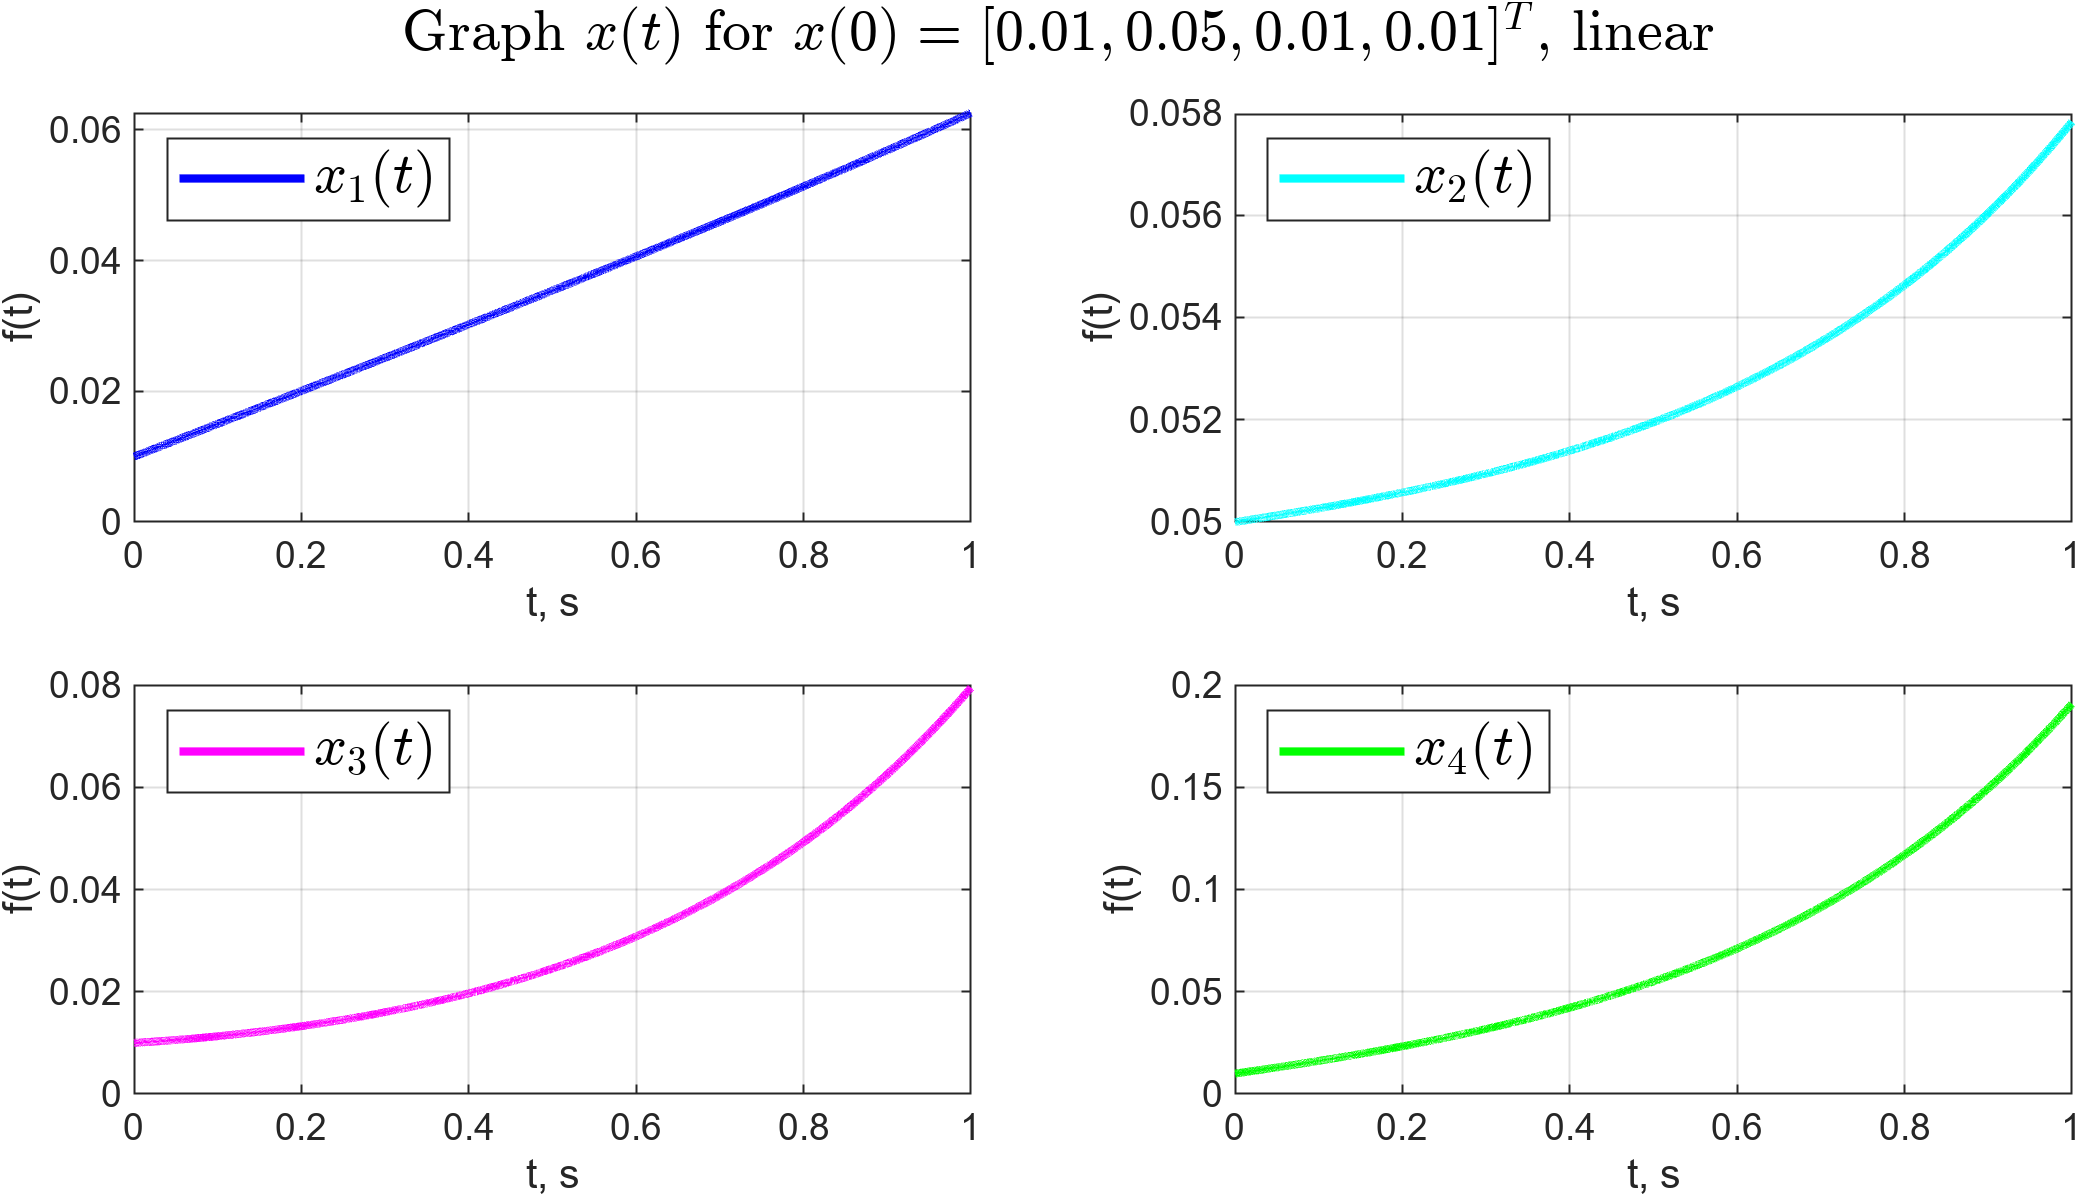
\includegraphics[width=1\linewidth]{pic/2_x_lin_03_sm.png}}
\caption{График вектора состояния линеаризованной системы, время моделирования $t=1$ с, начальные условия $x_{0_3}$.}
\label{2_x_lin_03_sm}
\end{figure}

\begin{figure}[!h]
\center{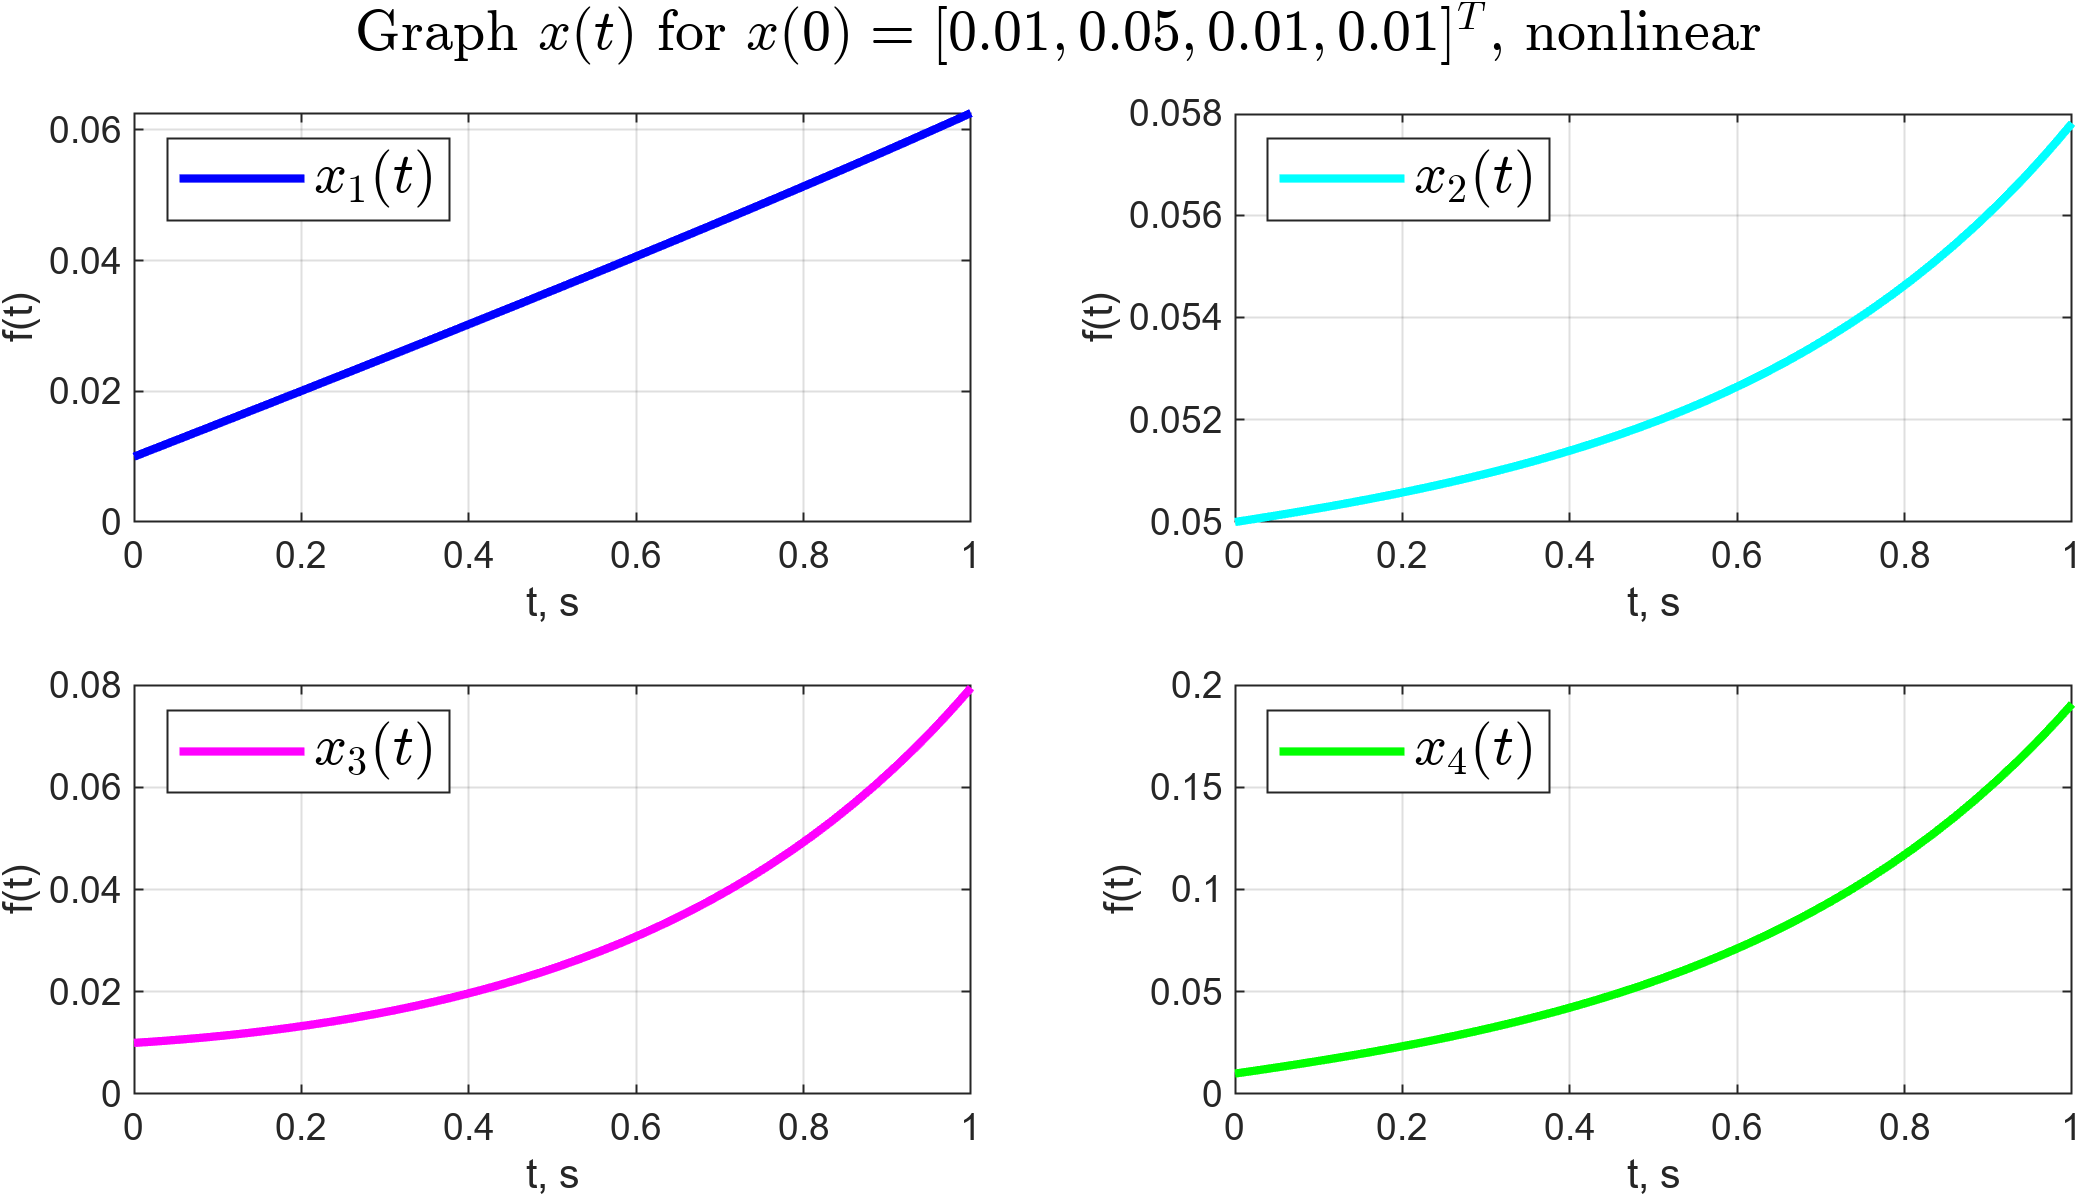
\includegraphics[width=1\linewidth]{pic/2_x_nlin_03_sm.png}}
\caption{График вектора состояния исходной системы, время моделирования $t=1$ с, начальные условия $x_{0_3}$.}
\label{2_x_nlin_03_sm}
\end{figure}

\begin{figure}[!h]
\center{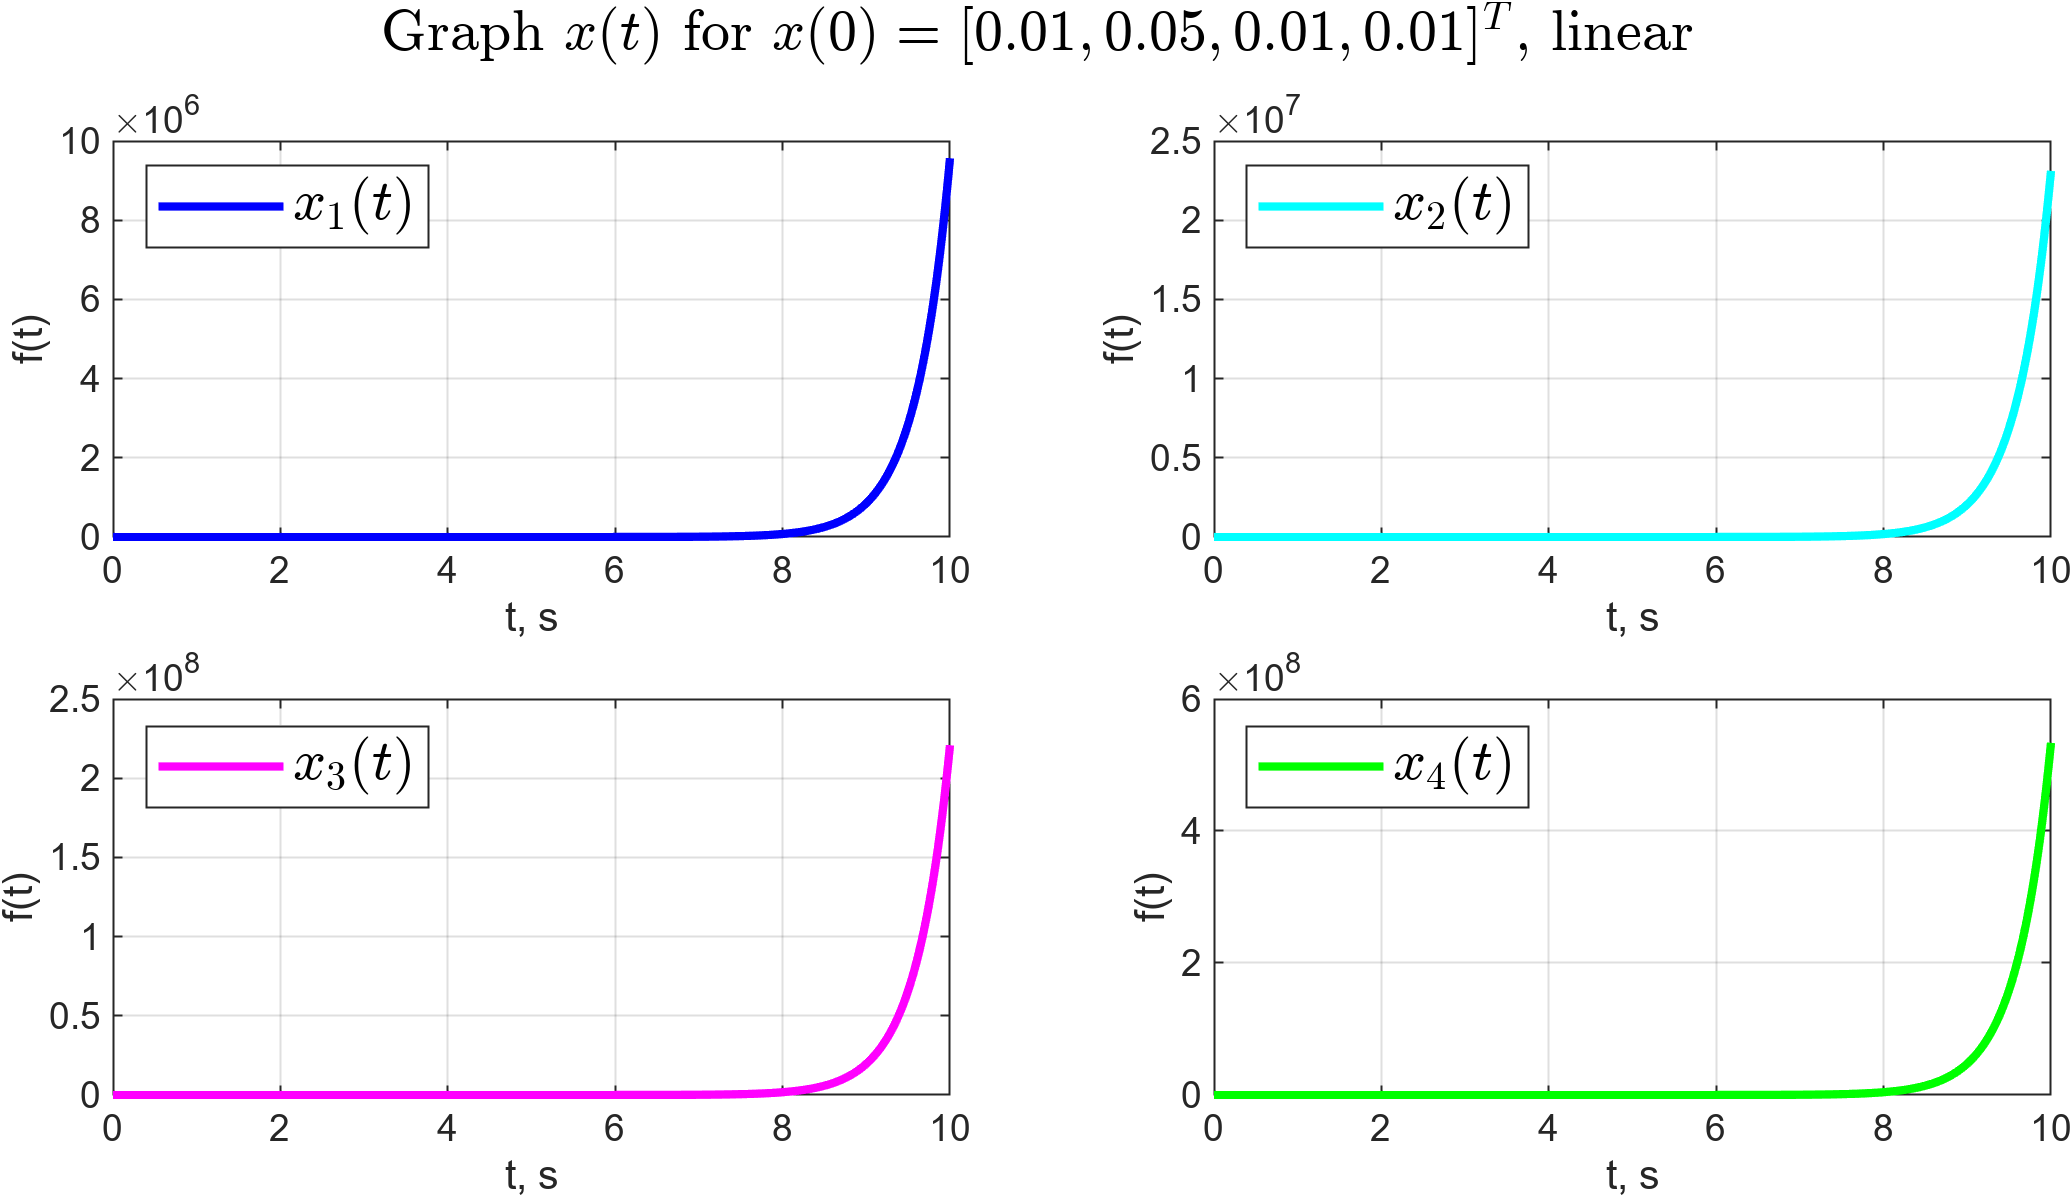
\includegraphics[width=1\linewidth]{pic/2_x_lin_03_lg.png}}
\caption{График вектора состояния линеаризованной системы, время моделирования $t=10$ с, начальные условия $x_{0_3}$.}
\label{2_x_lin_03_lg}
\end{figure}

\begin{figure}[!h]
\center{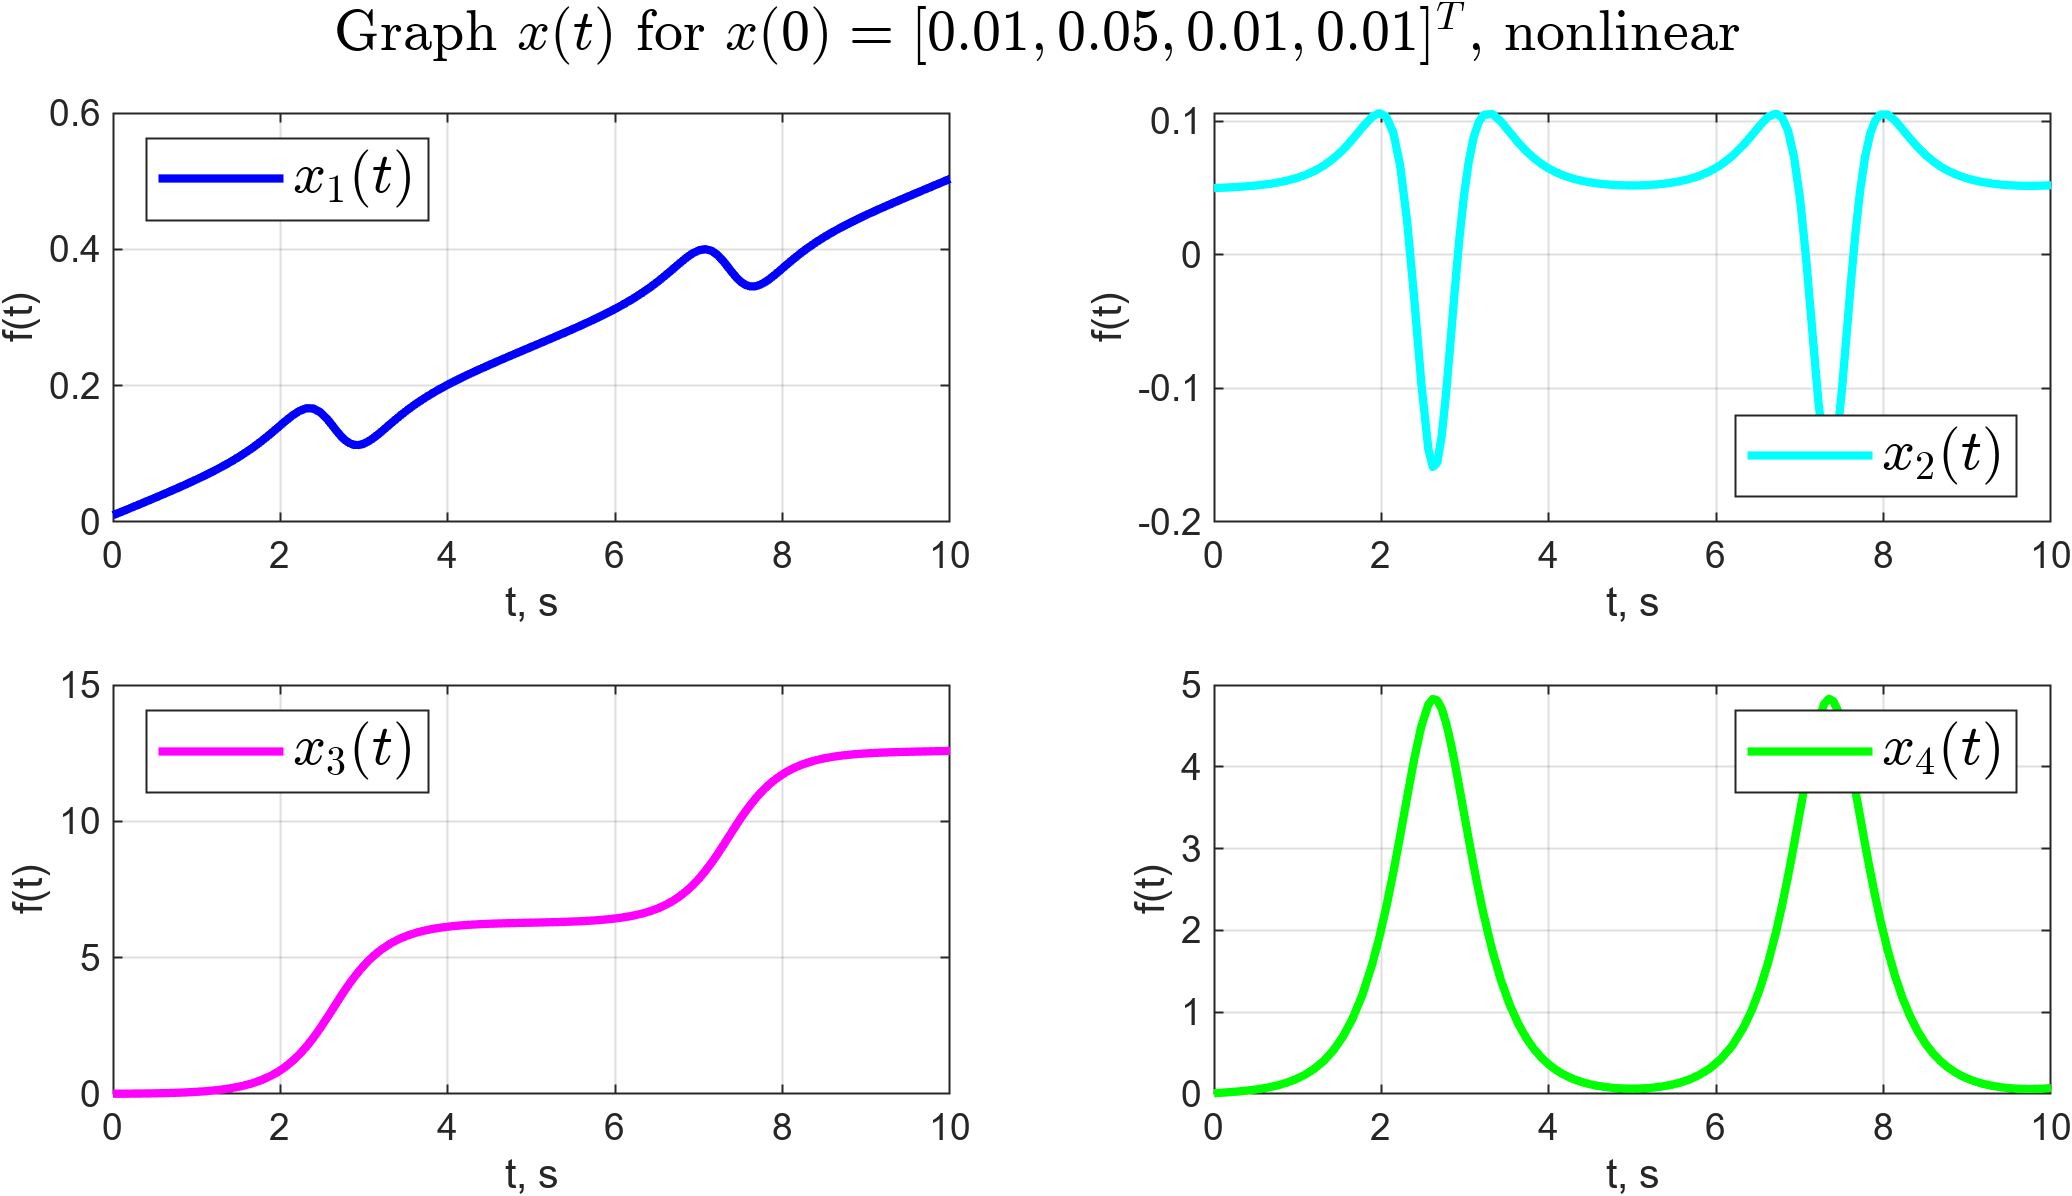
\includegraphics[width=1\linewidth]{pic/2_x_nlin_03_lg.png}}
\caption{График вектора состояния исходной системы, время моделирования $t=10$ с, начальные условия $x_{0_3}$.}
\label{2_x_nlin_03_lg}
\end{figure}
\newpage
\,
\newpage
 Для малого времени моделирования поведение линеаризованной и исходной систем вновь схожи, кроме того, заметим более быстрой рост координаты тележки, чем в предыдущих случаях. На небольшом промежутки времени также наблюдается траектория близкая к линейной, что не характерно для ранее рассмотренных начальных условий.
\endinput 
\chapter{Стабилизация маятника: модальное управление}
\label{ch:chap3}

\section{Синтез регулятора по состоянию}

Синтезируем регулятор вида 
\begin{equation}
    u = Kx
\end{equation}
основываясь на линеаризованной модели (\ref{1_model_lin}). В ходе анализа математической модели было выяснено, что система является полностью управляемой и спектр системы $\sigma(A) = \{ 0,\, \,  0, \, \,  2.4165,\, \,  -2.4165\}$.


Для нахождения матрицы регулятора $K$ будем решать систему, содержающую уравнение Сильвестра

\begin{equation}
    \label{3_sil_reg}
    \begin{cases}
        AP -P \Gamma = BY\\
        K = -YP^{-1}
    \end{cases}
\end{equation}
Запишем условия существования решения $P$: $\sigma(A) \cap \sigma(\Gamma) = \emptyset$, $(A,B)$ -- управляема, $(Y, \Gamma)$ -- наблюдаема. Заметим, что второе условие выполнено. 

Учтем то, что порядок ненулевых коэффициентов матрицы $B$ примерно $10^{-3}$, в то время, как матрица $A$ содержит элементы порядка единиц. Это может потребовать больших коэффициентов $K$, постараемся подобрать желаемый спектр так, чтобы требуемое управление было минимальным необходимым для стабилизации системы.  Зададимся желаемым спектром замкнутой системы ближе к мнимой оси $\sigma (A+BK) = \{-0.3, \, \, -0.25, \, \, -0.2, \, \, -0.15 \}$. Запишем подходящие матрицы $\Gamma$ и $Y$

\begin{equation}
    \Gamma = \begin{bmatrix}
        -0.3 & 0 & 0 & 0\\
        0 & -0.25 & 0 & 0\\
        0 & 0 & -0.2 & 0\\
        0 & 0 & 0 & -0.15
    \end{bmatrix}, 
    Y = \begin{bmatrix}
        1 & 1 & 1 & 1
    \end{bmatrix}
\end{equation}

Проверим, что пара $(Y, \Gamma)$ -- наблюдаема: составим матрицу наблюдаемости и определим ее ранг

\begin{multline}
    V = \begin{bmatrix}
        Y\\ Y \Gamma \\ Y \Gamma^2 \\ Y \Gamma^3
    \end{bmatrix} = \begin{bmatrix}
        1&	1 &1&	1\\
-0.3&-0.25&-0.2&-0.15\\
0.09&	0.0625	&0.04&0.0225\\
-0.027&	-0.0156	&-0.008&	-0.0034
    \end{bmatrix} \Rightarrow\\\Rightarrow rank(V) = 4
\end{multline}
Ранг матрицы наблюдаемости равен размерности системы, следовательно, пара $(Y, \Gamma)$ -- наблюдаема.

Синтезируем матрицу $K$ решив систему (\ref{3_sil_reg})

\begin{equation}
    K = \begin{bmatrix}
        0.10548 & 2.0042& -2822.6 & -417.37
    \end{bmatrix}
\end{equation}

Исследуем работоспособность синтезированного регулятора при управлении нелинейной системой (\ref{1_model_full}) с различными начальными условиями при $f=0$. Сначала проверим начальные условия из главы 2:

$$x_{0_1} = \begin{bmatrix}
     0.01\\
    0.01\\
    0.01\\
    0.05
\end{bmatrix},  x_{0_2} = \begin{bmatrix}
    0.01\\
    0.01\\
    0.05\\
    0.01
\end{bmatrix},  x_{0_3} = \begin{bmatrix}
    0.01\\
    0.05\\
    0.01\\
    0.01
\end{bmatrix}$$

При начальных условиях $x_{0_1}$, $x_{0_2}$ и $x_{0_3}$ вектор состояния нелинейной системы с течением времени сходится к нулю, при данных условиях система стабилизируется. Так как при линеаризации мы считали малыми угол отклонения маятника от вертикали и угловую скорость, зададим вектор начальных условий с большим начальным углом отклонения $$x_{0_4} = \begin{bmatrix}
   0.01 & 0.01 & \frac{\pi}{4} & 0.01 
\end{bmatrix}^T$$ и вектор с существенной начальной угловой скоростью $$x_{0_5} = \begin{bmatrix}
    0.01 & 0.01 & 0.01& 1
\end{bmatrix}^T$$



\begin{figure}[!h]
\center{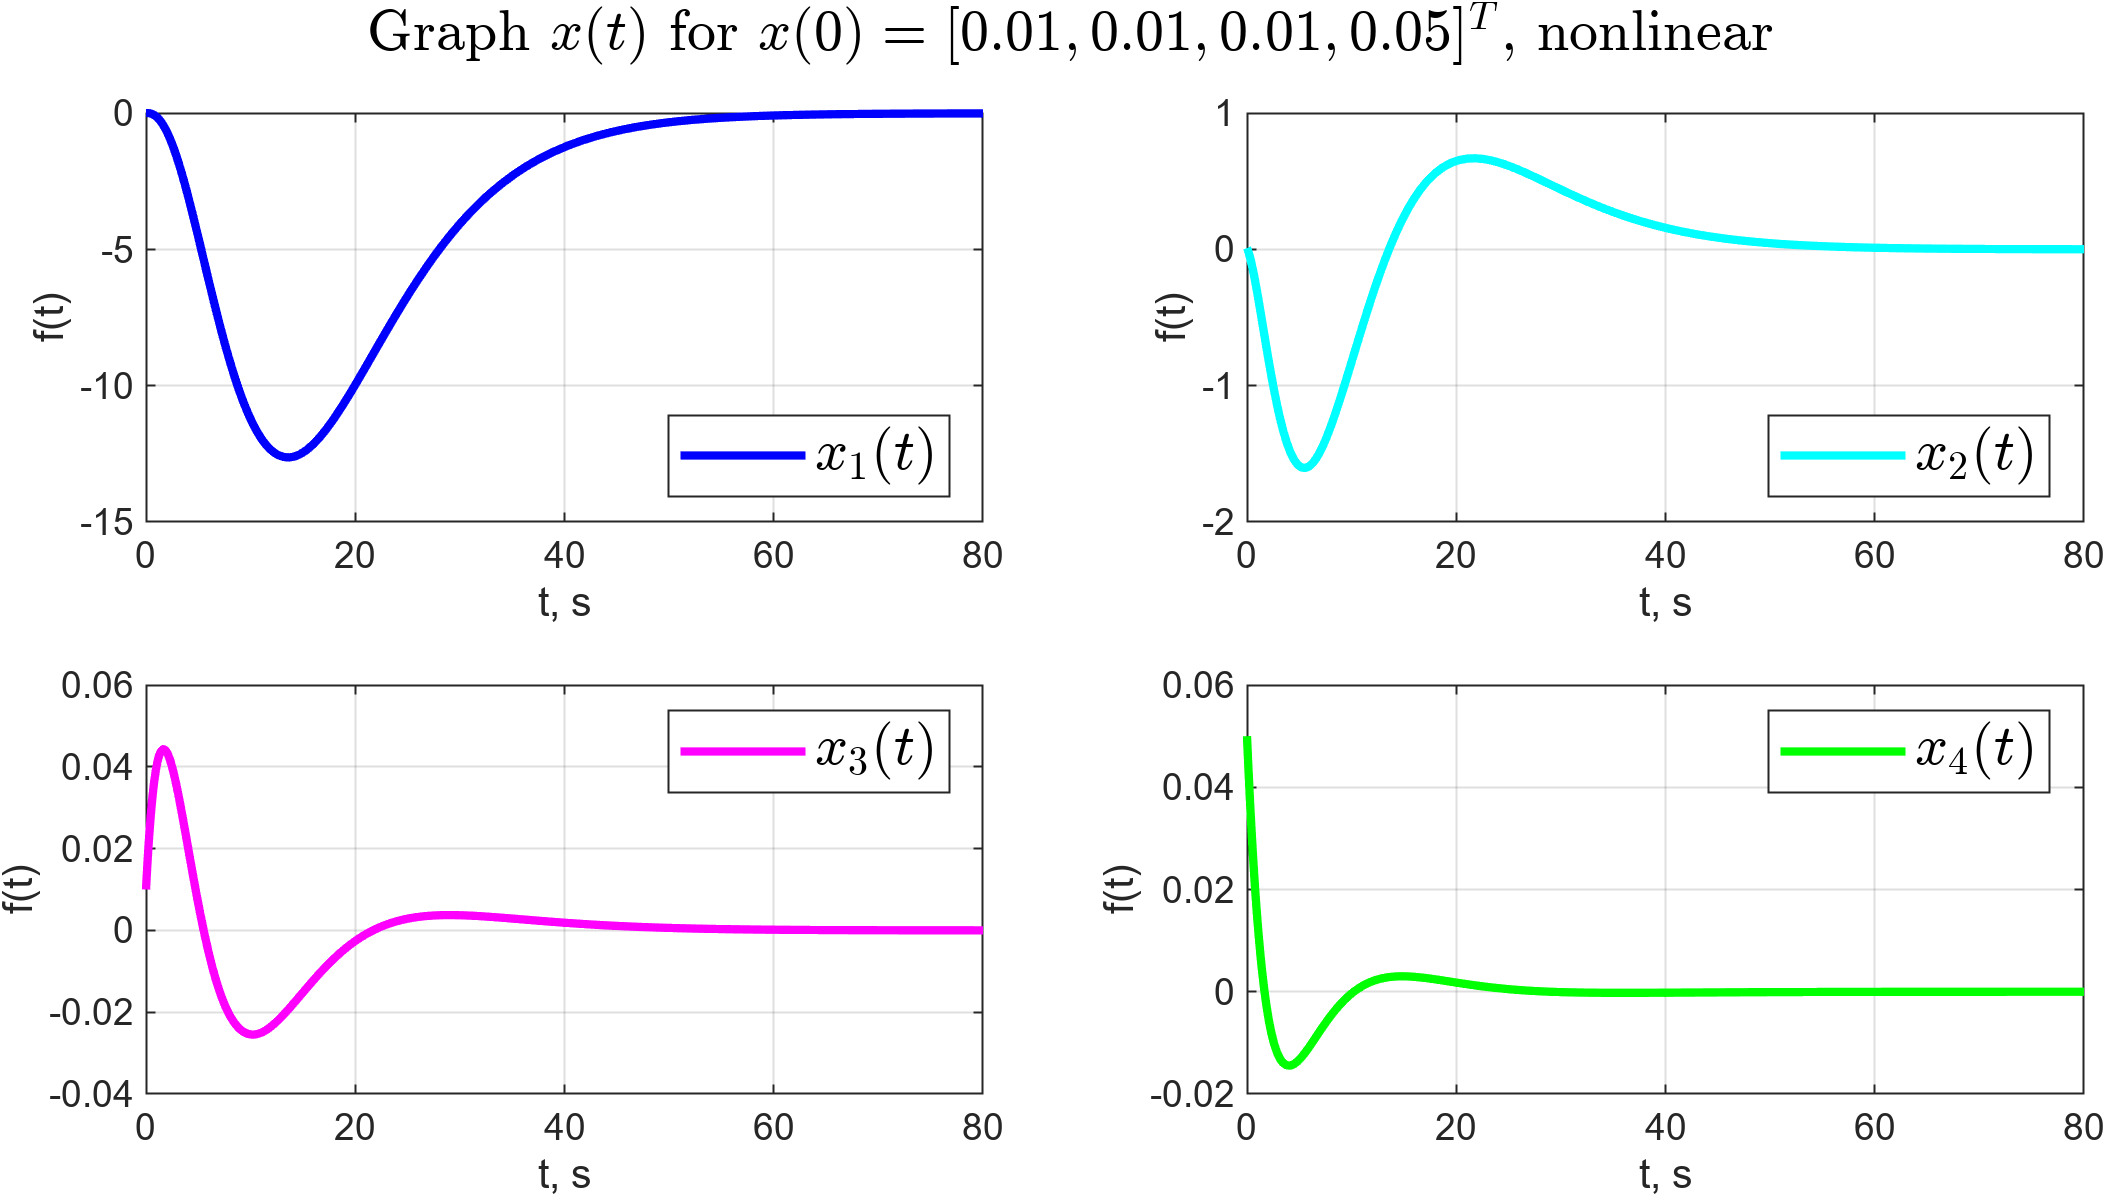
\includegraphics[width=1\linewidth]{pic/3_x_nlin_01_lg.png}}
\caption{График вектора состояния нелинейной системы, начальные условия $x_{01}$.}
\label{3_x_nlin_01_lg}
\end{figure}


\begin{figure}[!h]
\center{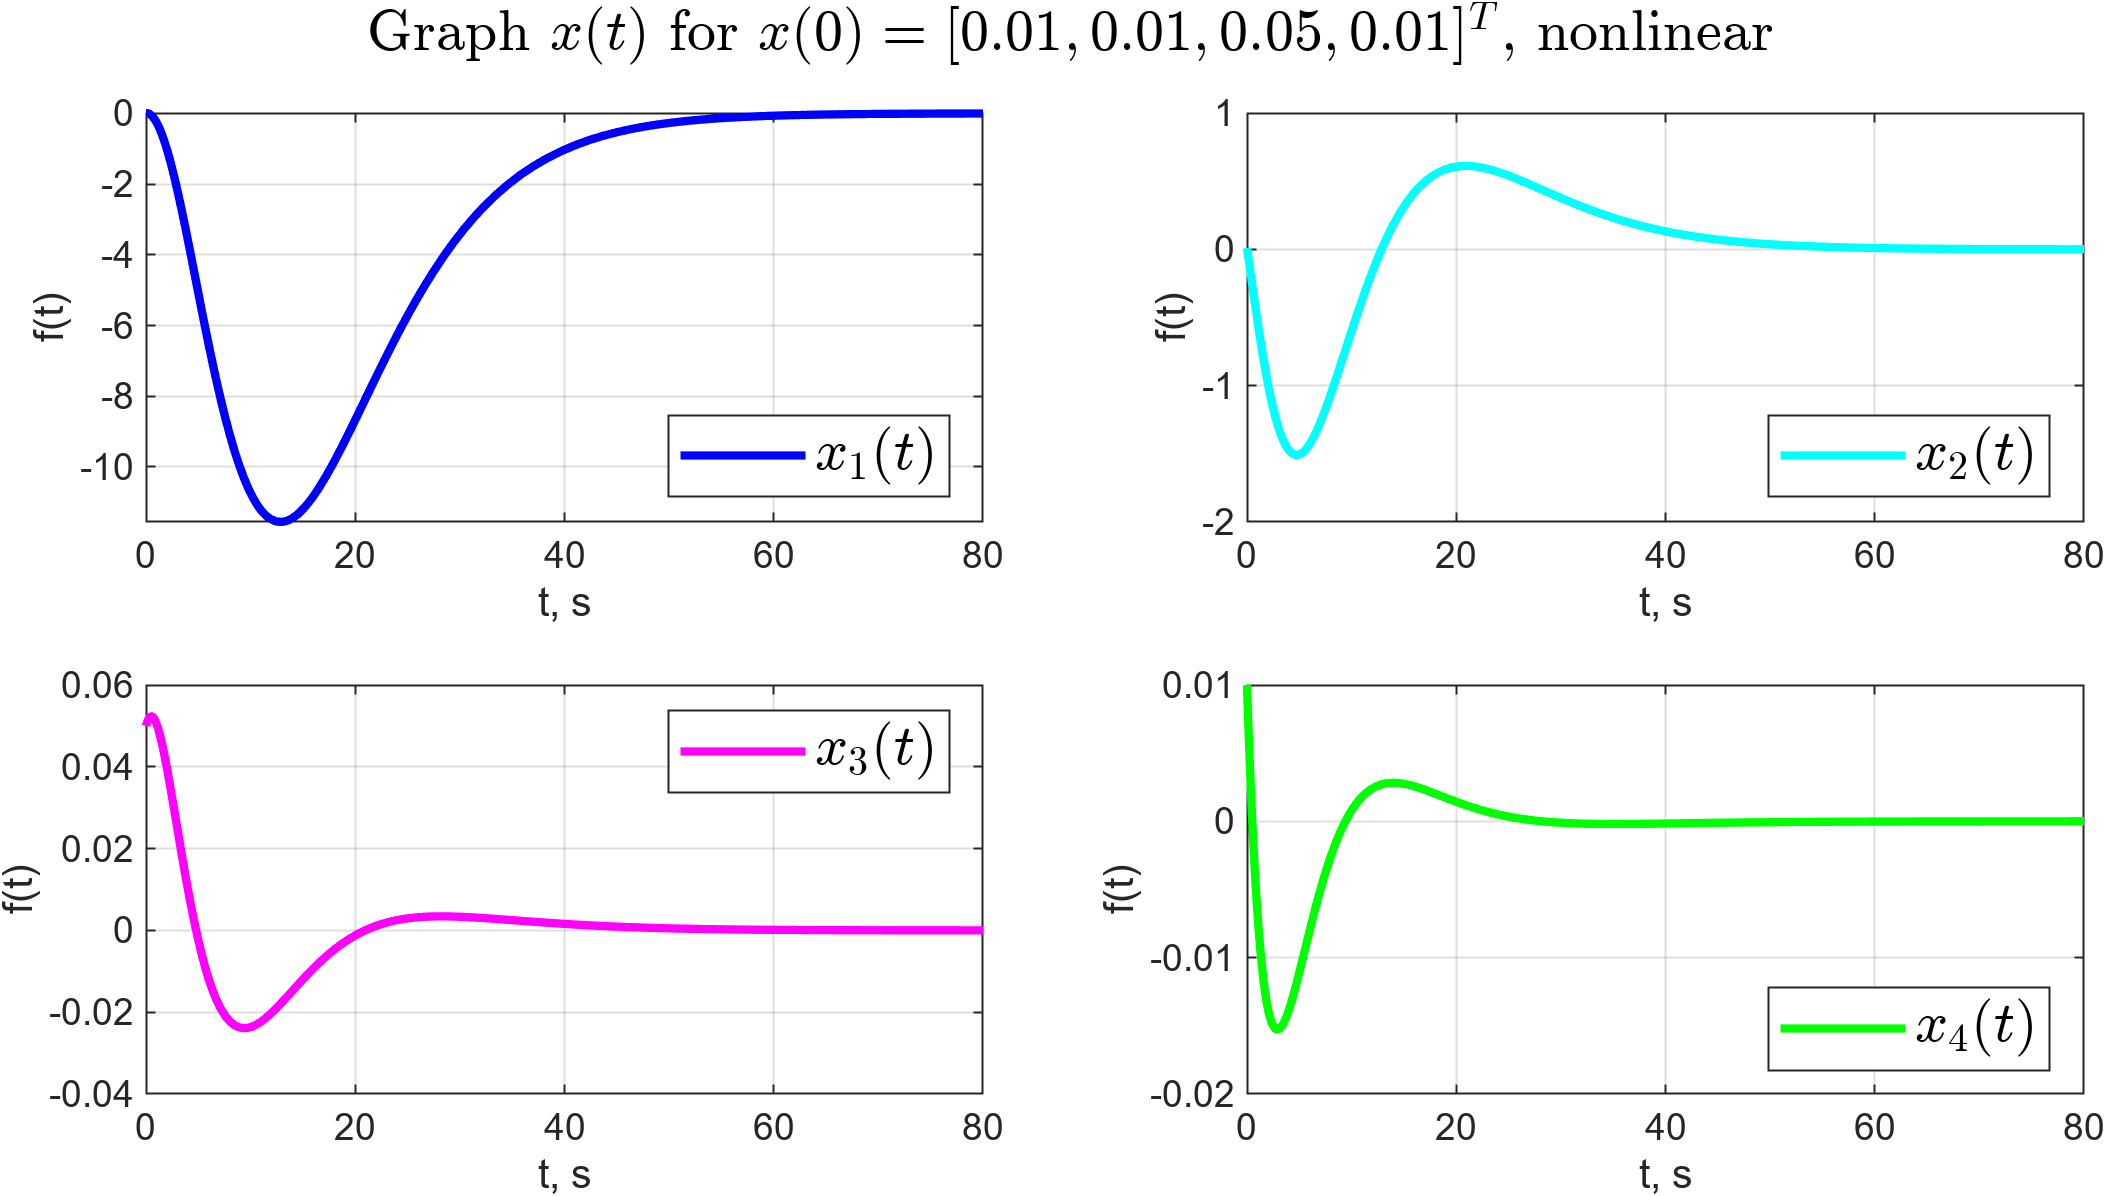
\includegraphics[width=1\linewidth]{pic/3_x_nlin_02_lg.png}}
\caption{График вектора состояния нелинейной системы, начальные условия $x_{02}$.}
\label{3_x_nlin_02_lg}
\end{figure}

\begin{figure}[!h]
\center{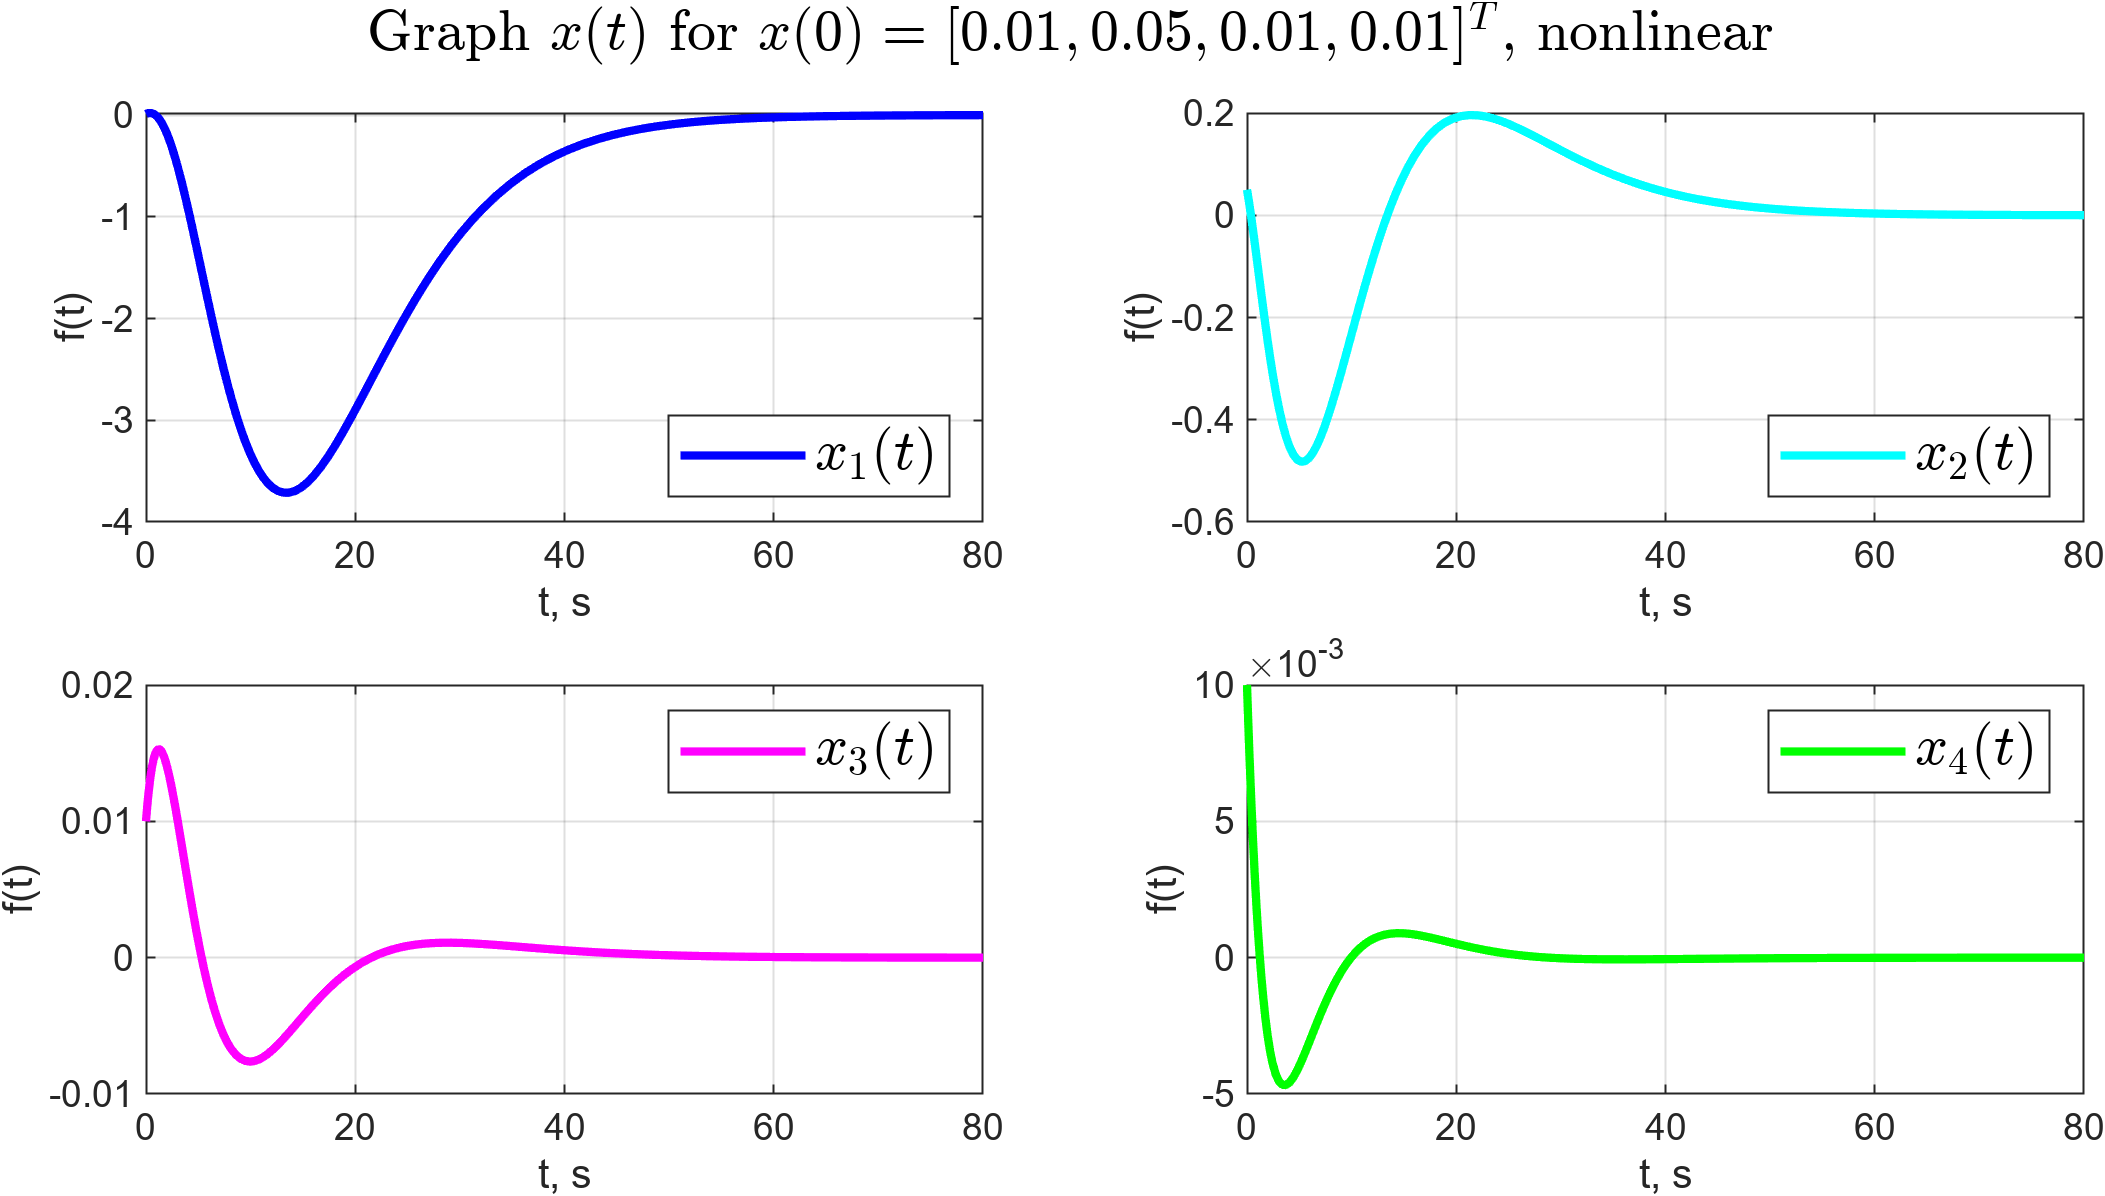
\includegraphics[width=1\linewidth]{pic/3_x_nlin_03_lg.png}}
\caption{График вектора состояния нелинейной системы, начальные условия $x_{03}$.}
\label{3_x_nlin_03_lg}
\end{figure}

\begin{figure}[!h]
\center{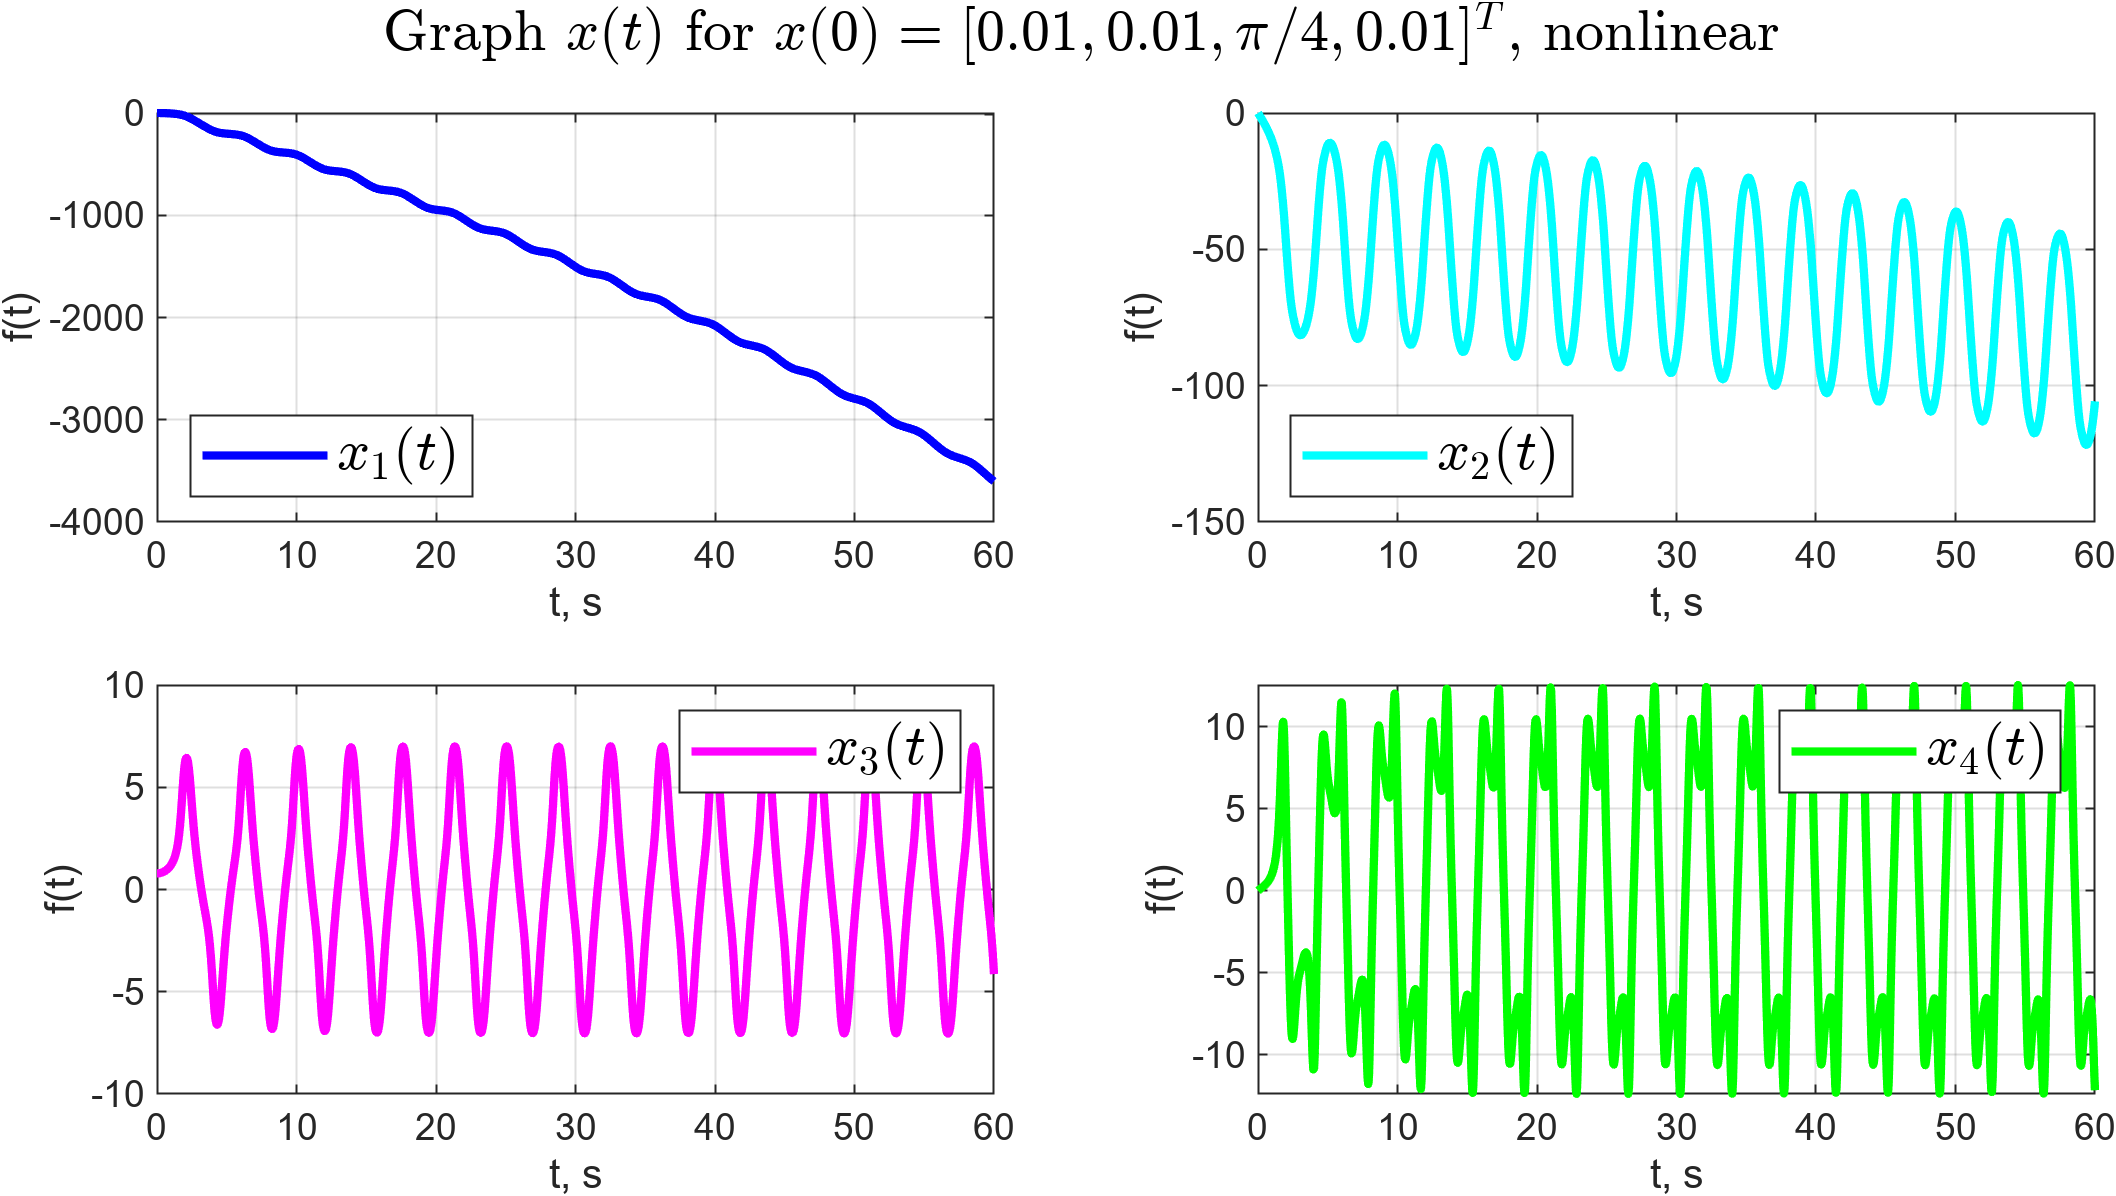
\includegraphics[width=1\linewidth]{pic/3_x_nlin_04_lg.png}}
\caption{График вектора состояния нелинейной системы, начальные условия $x_{04}$.}
\label{3_x_nlin_04_lg}
\end{figure}

\newpage
\,
\newpage
Заметим, что действительно при задании довольно большого угла начального отклонения маятника, система уже не стабилизируется синтезированным регулятором (рисунок \ref{3_x_nlin_04_lg}), также как и при большем начальном значении угловой скорости (рисунок \ref{3_x_nlin_05_lg}). 

\begin{figure}[!h]
\center{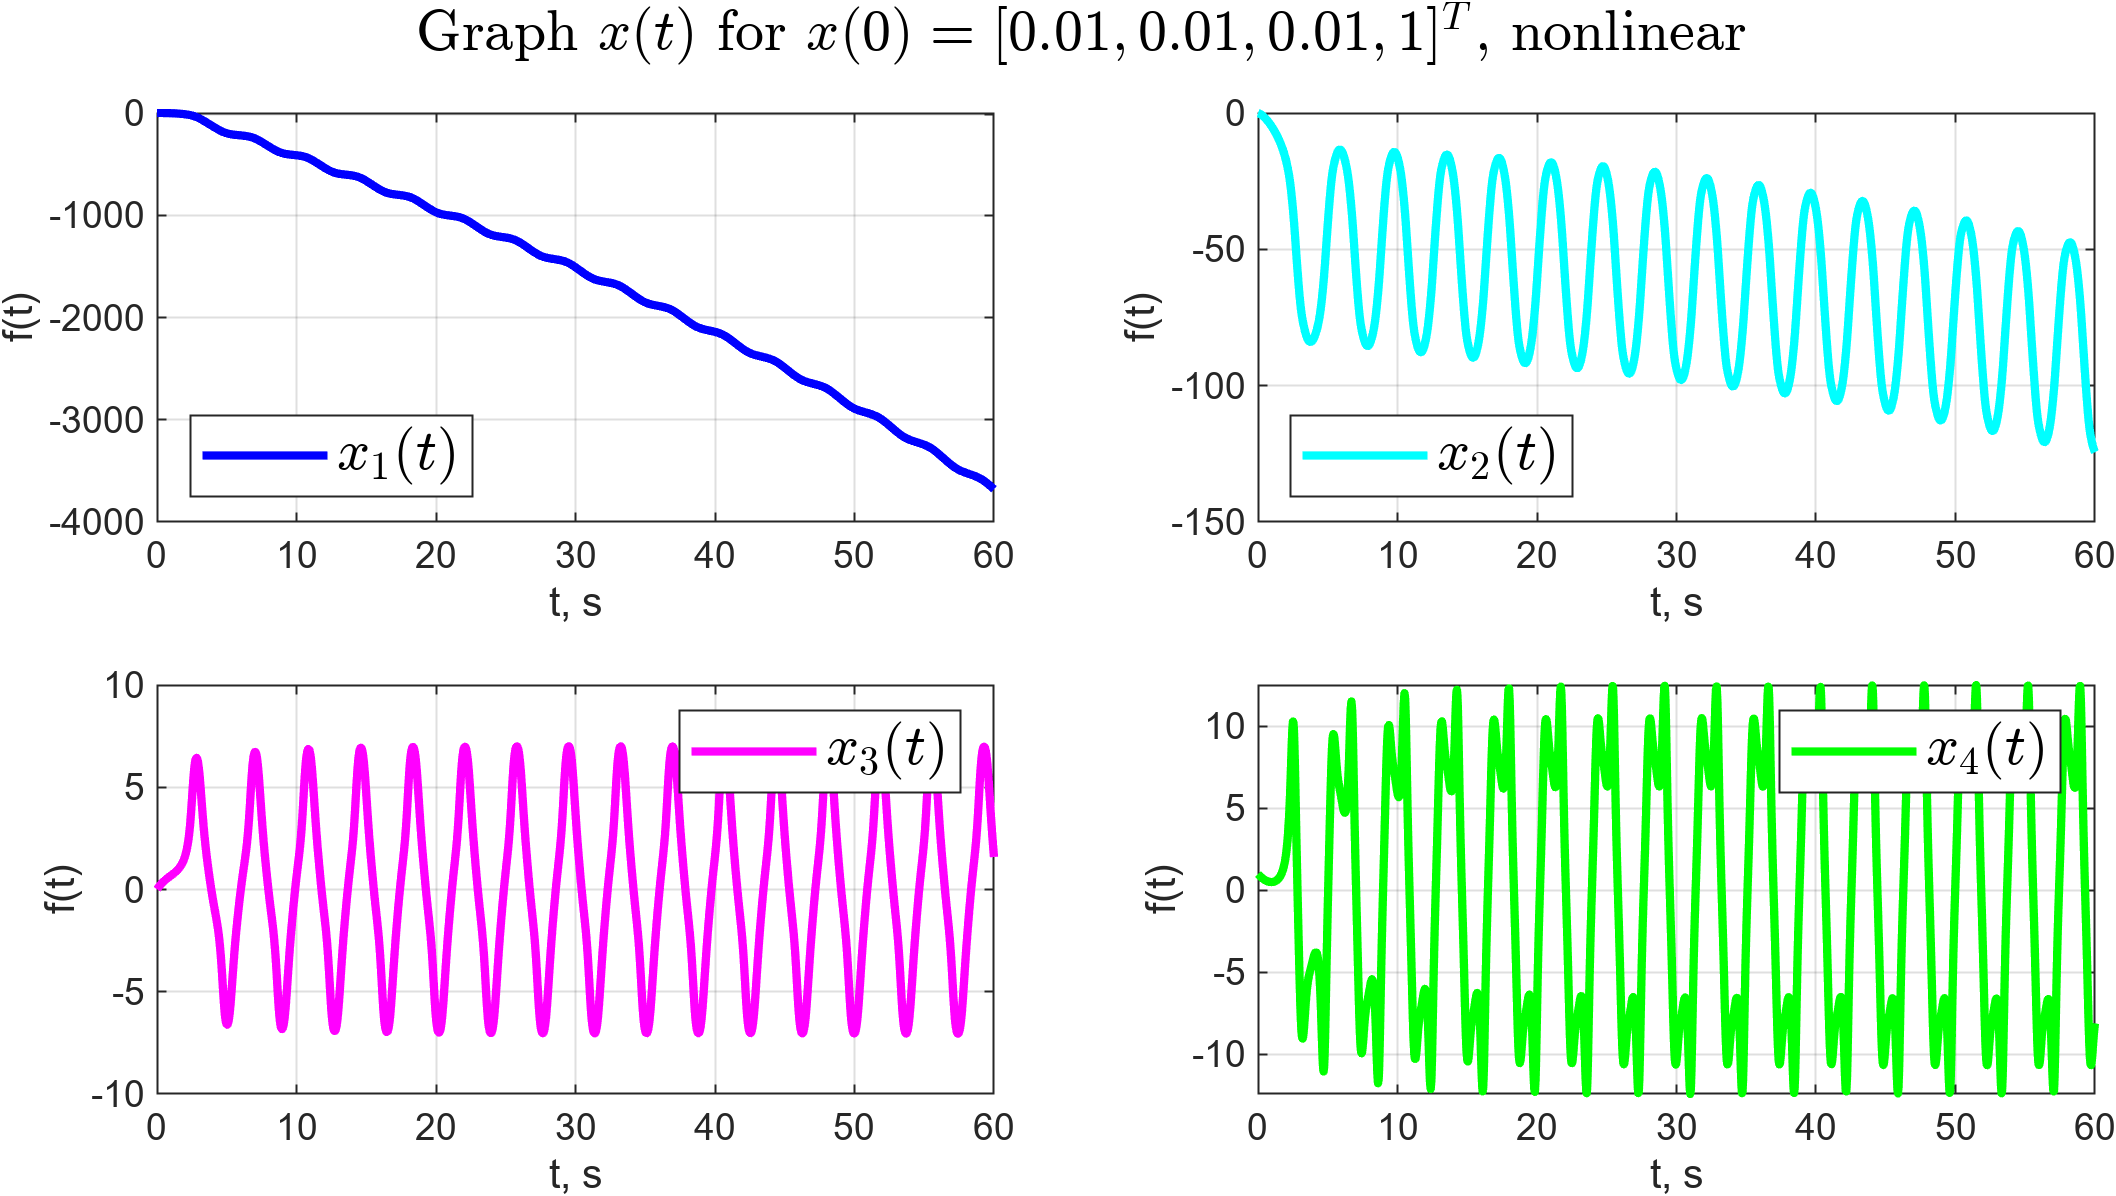
\includegraphics[width=1\linewidth]{pic/3_x_nlin_05_lg.png}}
\caption{График вектора состояния нелинейной системы, начальные условия $x_{05}$.}
\label{3_x_nlin_05_lg}
\end{figure}

Заметим также, что система нестабилизируется также при сильном увеличении начального значения скорости тележки (рисунок \ref{3_x_nlin_06_lg}) $$x_{06} = \begin{bmatrix}
    0.01 & 25 & 0.01 & 0.01
\end{bmatrix}^T$$ 

\begin{figure}[!h]
\center{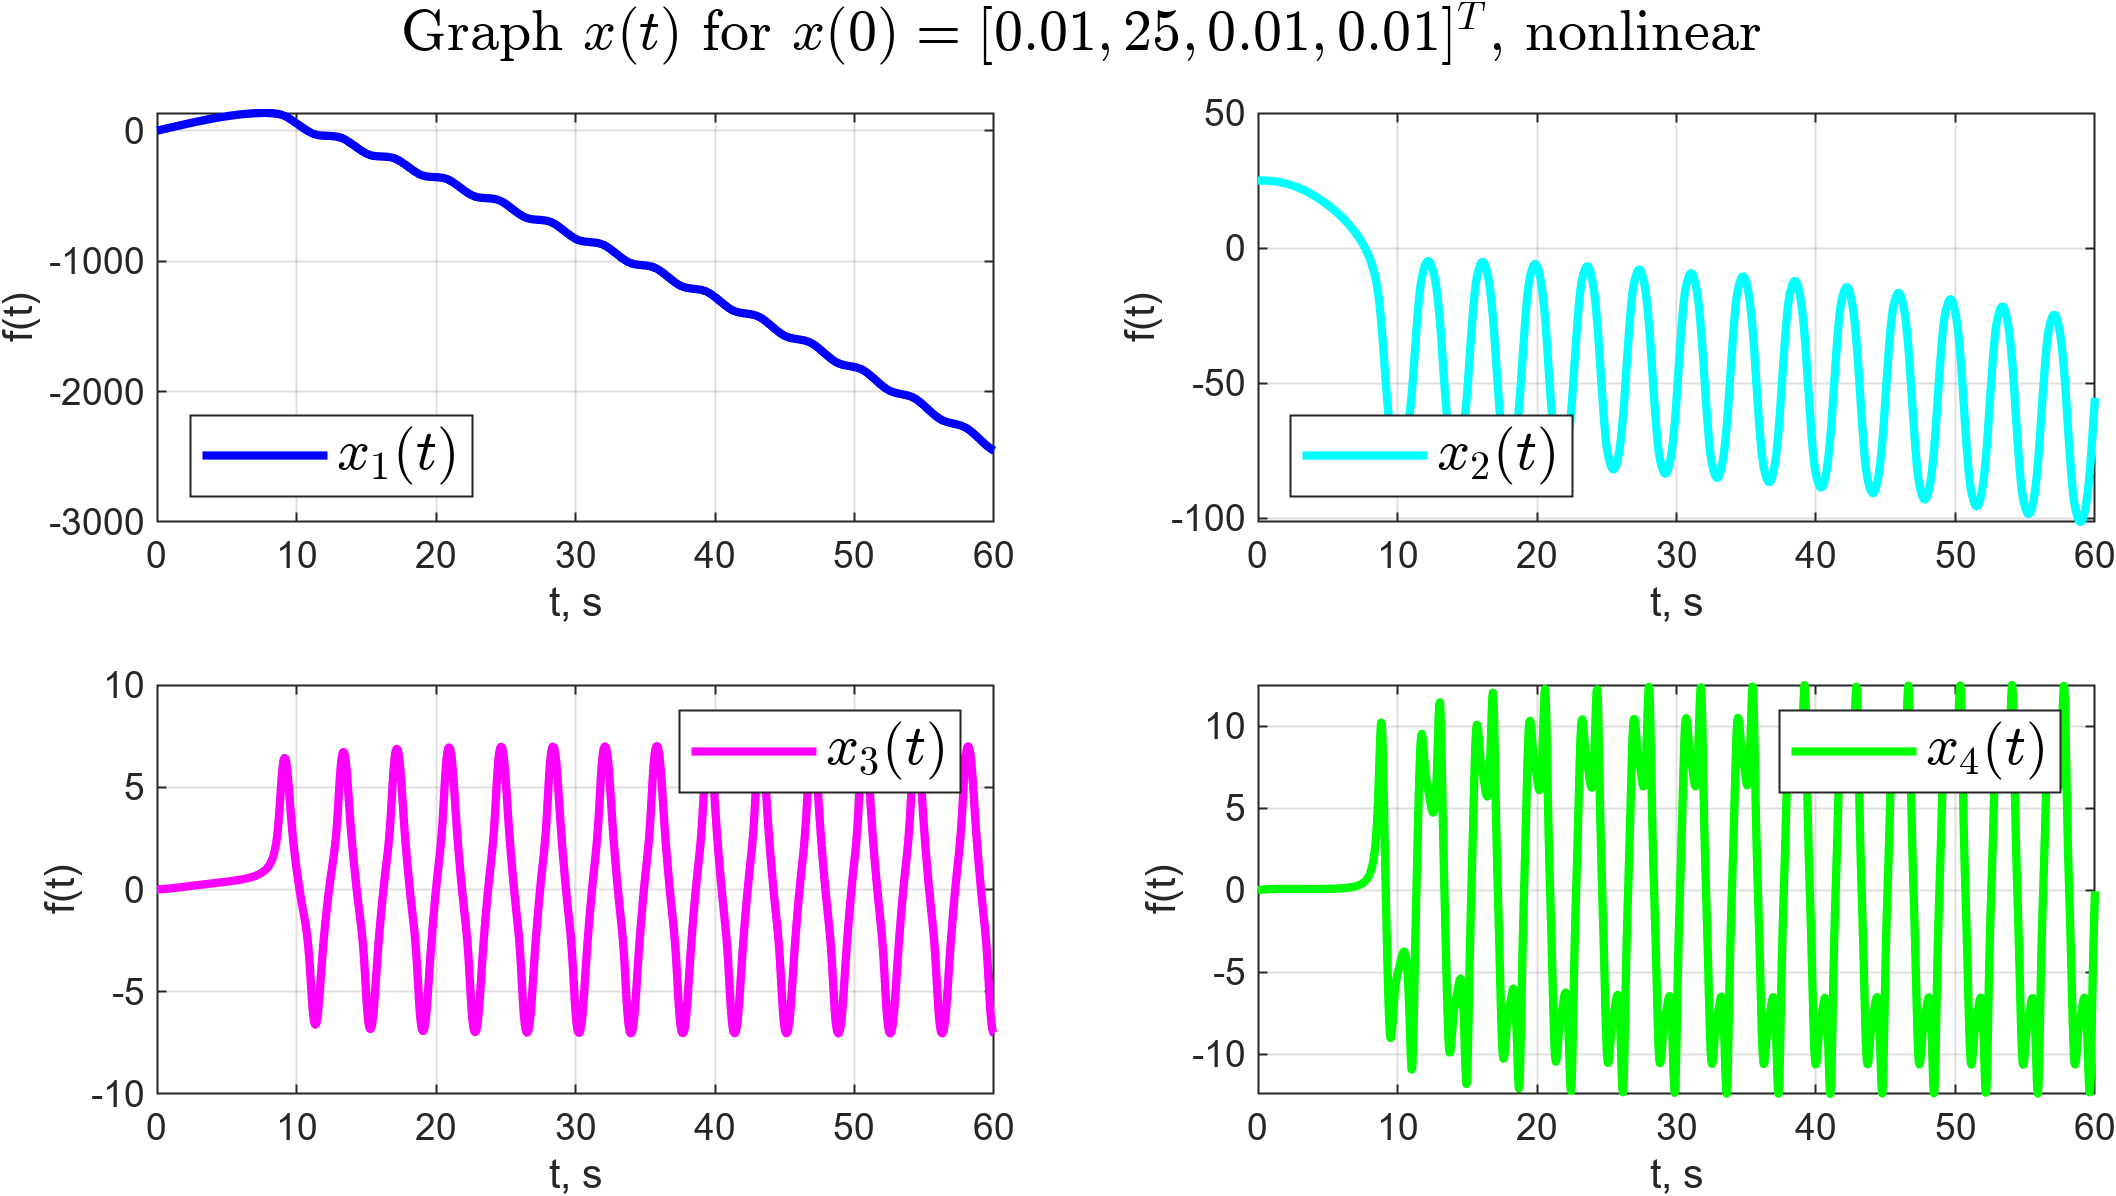
\includegraphics[width=1\linewidth]{pic/3_x_nlin_06_lg.png}}
\caption{График вектора состояния нелинейной системы, начальные условия $x_{06}$.}
\label{3_x_nlin_06_lg}
\end{figure}

Убедимся в том, что изменение начального значения координаты тележки до 100, не препятствует успешной стабилизации системы (рисунок \ref{3_x_nlin_07_lg})
$$x_{07} = \begin{bmatrix}
    100 & 0.01 & 0.01 & 0.01
\end{bmatrix}^T$$

\begin{figure}[!h]
\center{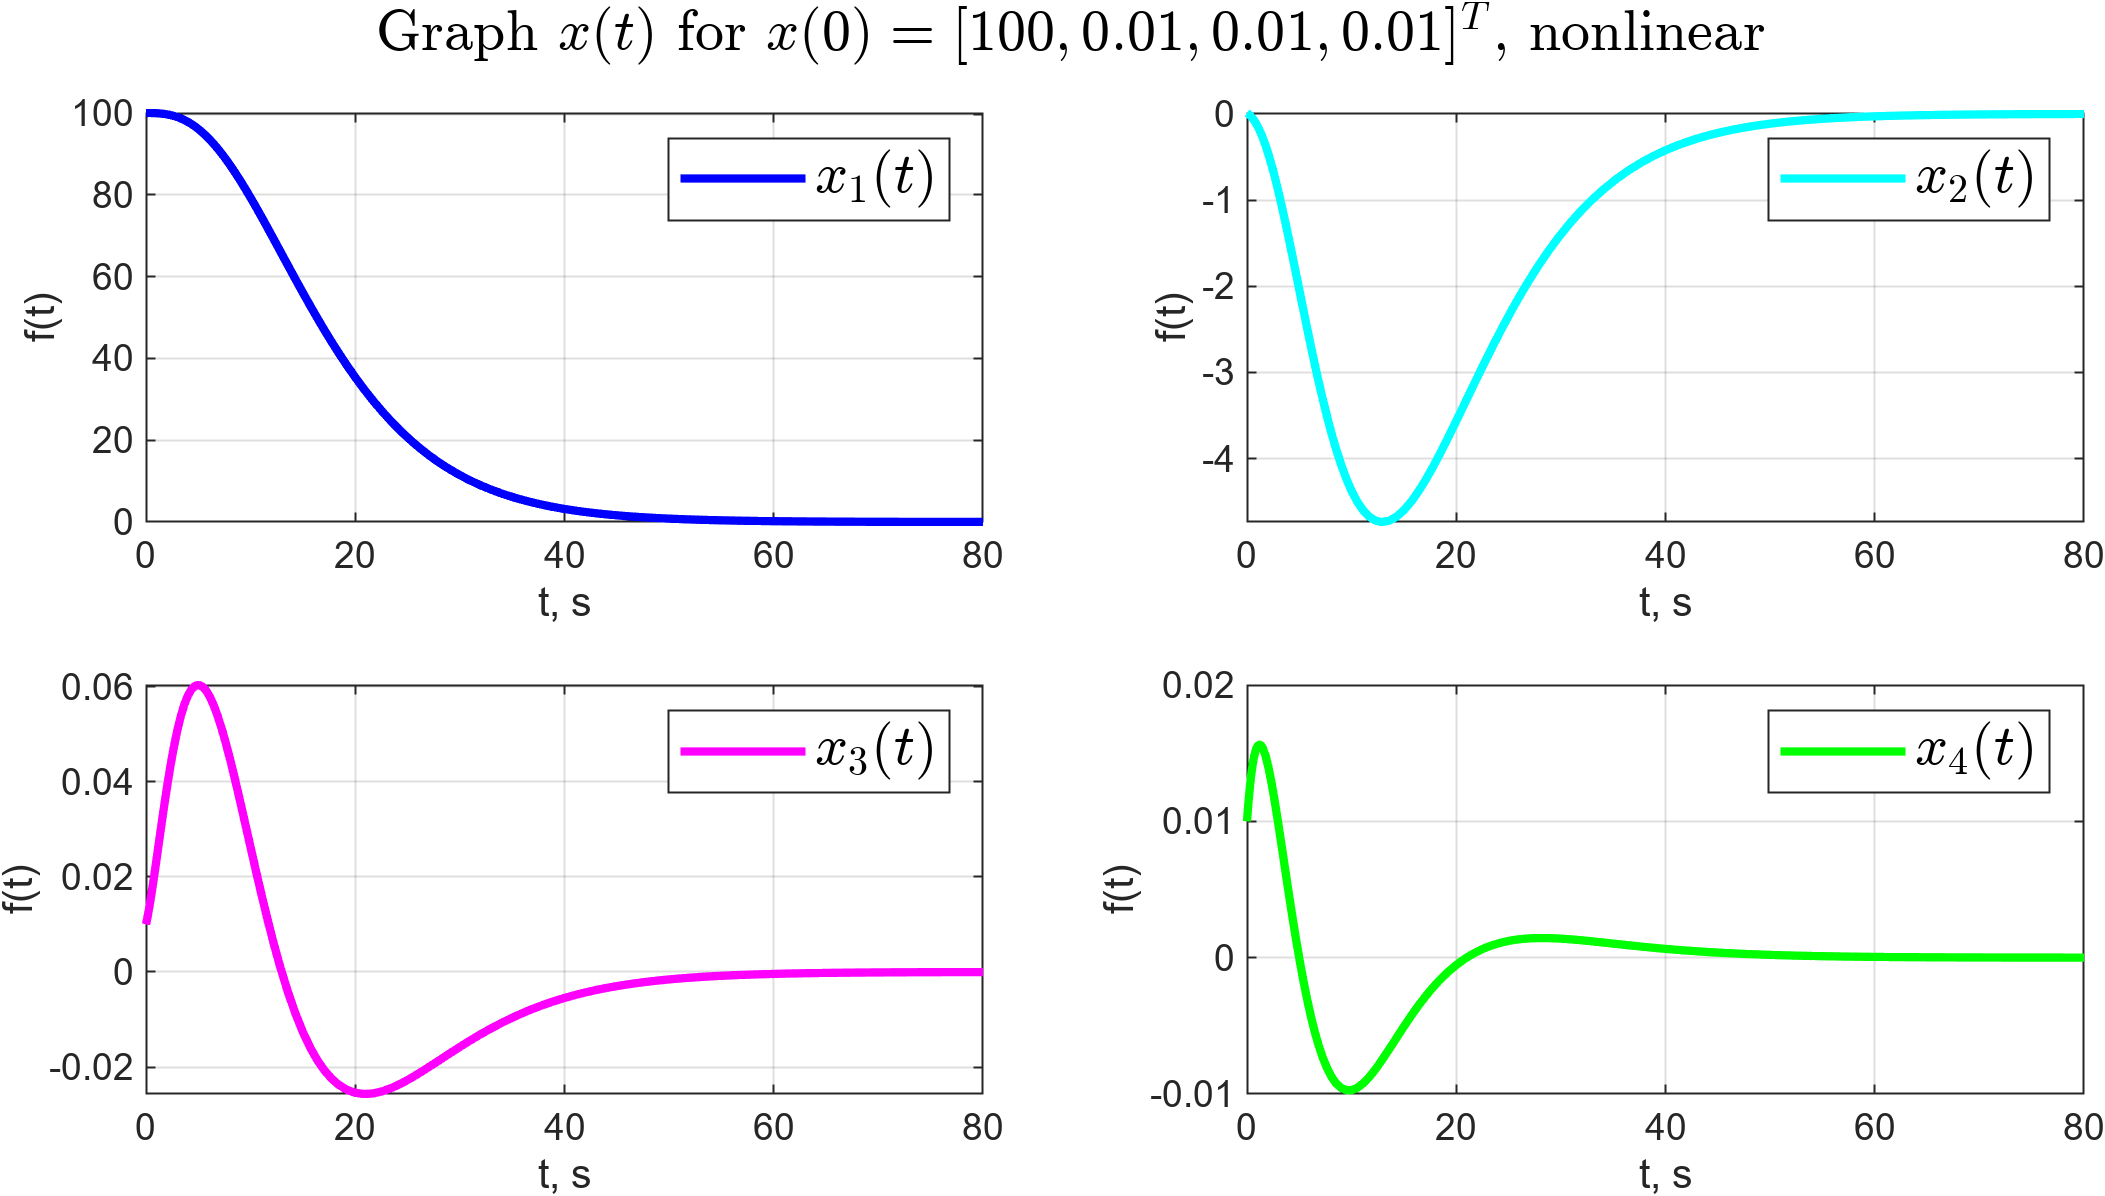
\includegraphics[width=1\linewidth]{pic/3_x_nlin_07_lg.png}}
\caption{График вектора состояния нелинейной системы, начальные условия $x_{07}$.}
\label{3_x_nlin_07_lg}
\end{figure}

Однако при повышении начального значения координаты тележки до 1000 стабилизировать систему с помощью синтезированного регулятора не удается (рисунок \ref{3_x_nlin_08_lg})
$$x_{08} = \begin{bmatrix}
    1000 & 0.01 & 0.01 & 0.01
\end{bmatrix}$$

\begin{figure}[!h]
\center{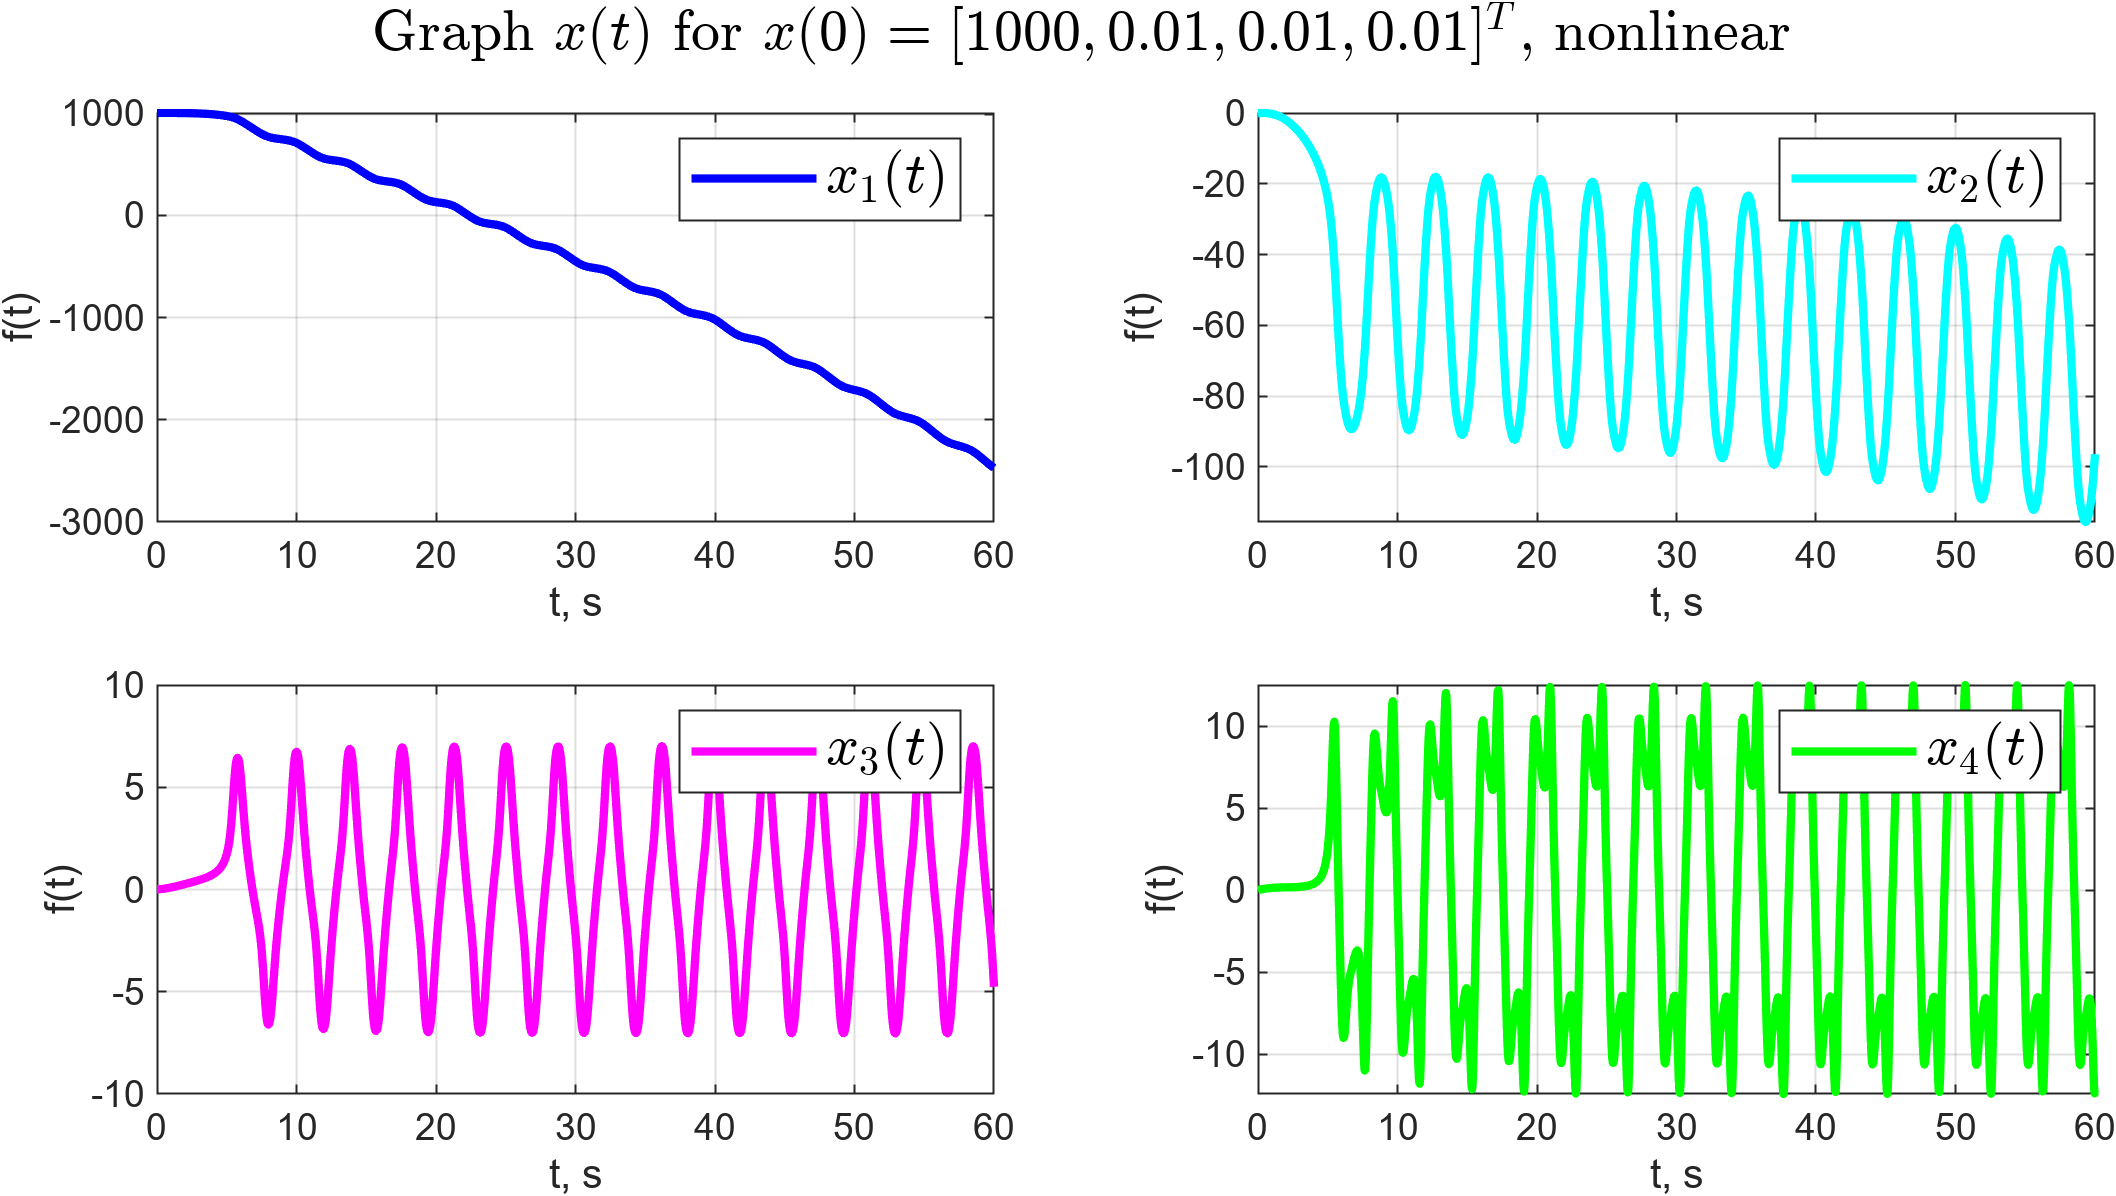
\includegraphics[width=1\linewidth]{pic/3_x_nlin_08_lg.png}}
\caption{График вектора состояния нелинейной системы, начальные условия $x_{08}$.}
\label{3_x_nlin_08_lg}
\end{figure}

\newpage
\subsection{Краткий вывод}
При начальных условиях, близких к нулю (наборы $x_{01}$, $x_{02}$, $x_{03}$), синтезированный регулятор позволяет стабилизировать систему. Начальные условия для угла отклонения и угловой скорости не позволяют стабилизировать систему, если принимают значения порядка единицы. В ходе дополнительного моделирования было выяснено, что критическим значением начальной скорости тележки, при котором регулятор не работает, является $\approx 18$ м/с. Критическим значением начальной координаты тележки, при котором перестает работать регулятор, является $\approx 400$ м. 


\section{Исследование регулятора по состоянию}

Исследуем влияние выбранных собственных чисел на максимальное отклонение маятника от вертикали, максимальное горизонтальное смещение тележки и максимальное значение управляющего сигнала при управлении нелинейной системой (\ref{1_model_full}).

Будем рассматривать следующие спектры замкнутой системы

\begin{equation*}
  \begin{matrix}
      \sigma_1 = \{ -0.3, -0.25, -0.2, -0.15 \}, & \sigma_2 = \{ -3, -2.5, -2, -1.5 \},\\
      \sigma_3 = \{ -1, -2, -3 \pm 3i \}, & \sigma_4 = \{ -10, -20, -30 \pm 10i \}
 \end{matrix}
\end{equation*}

в качестве начальных условий примем вектор $$x(0) = \begin{bmatrix}
    0.01&&
    0.01&&
    0.01&&
    0.01
\end{bmatrix}^T$$

\begin{table}[h]
\centering
\caption{Значения управления \( u(t) \) и состояний системы}
\label{tab:results}
\begin{tabular}{ccccc}
\toprule
Спектр & $\max |\varphi|$ & $\max |a|$ & $\max |u|$ \\
\midrule
$\sigma_1$  &  0.0152  &  3.9533  &  43.4049  \\
$\sigma_2$  &  0.0101  &  0.0389  &  227.1943  \\
$\sigma_3$  &  0.0101  &  0.0329  &  277.5976  \\
$\sigma_4$  &  0.0499  &  0.0935  &  96295  \\
\bottomrule
\end{tabular}
\end{table}

\begin{figure}[!h]
\center{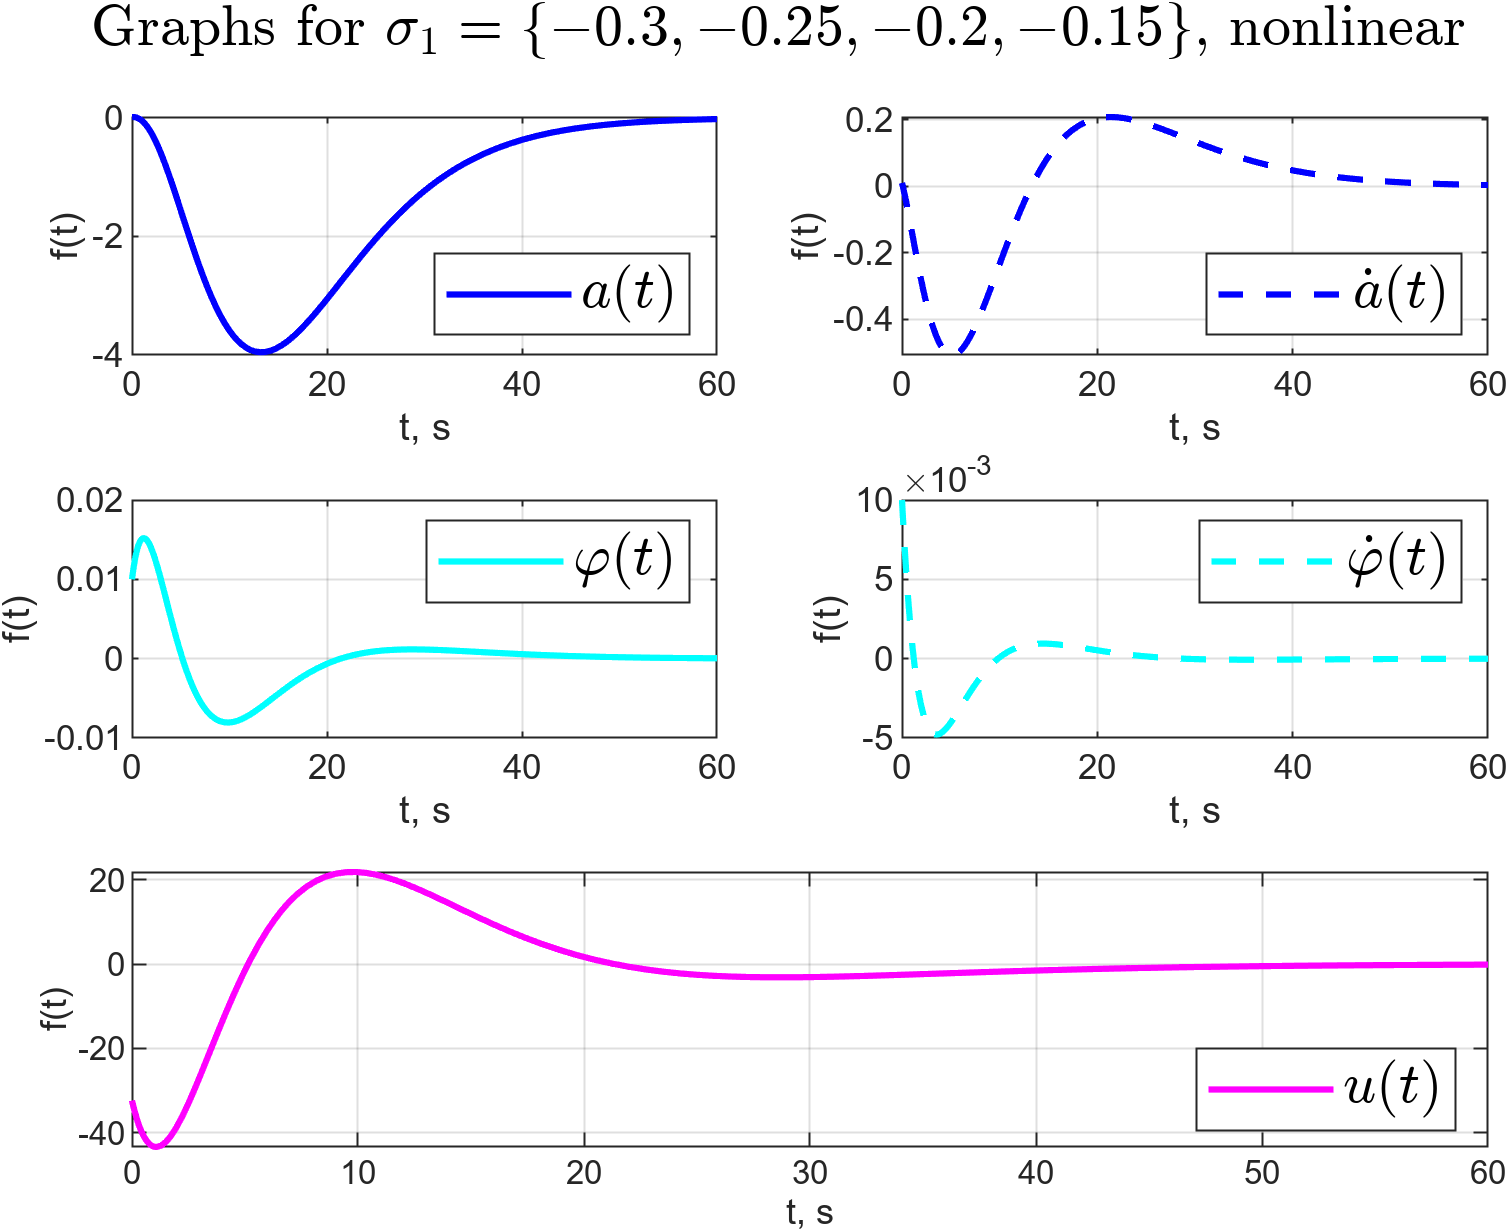
\includegraphics[width=1\linewidth]{pic/3_x_nlin_s1.png}}
\caption{Графики компонент вектора состояния системы и $u(t)$ для $\sigma_1$.}
\label{3_x_nlin_s1}
\end{figure}

\begin{figure}[!h]
\center{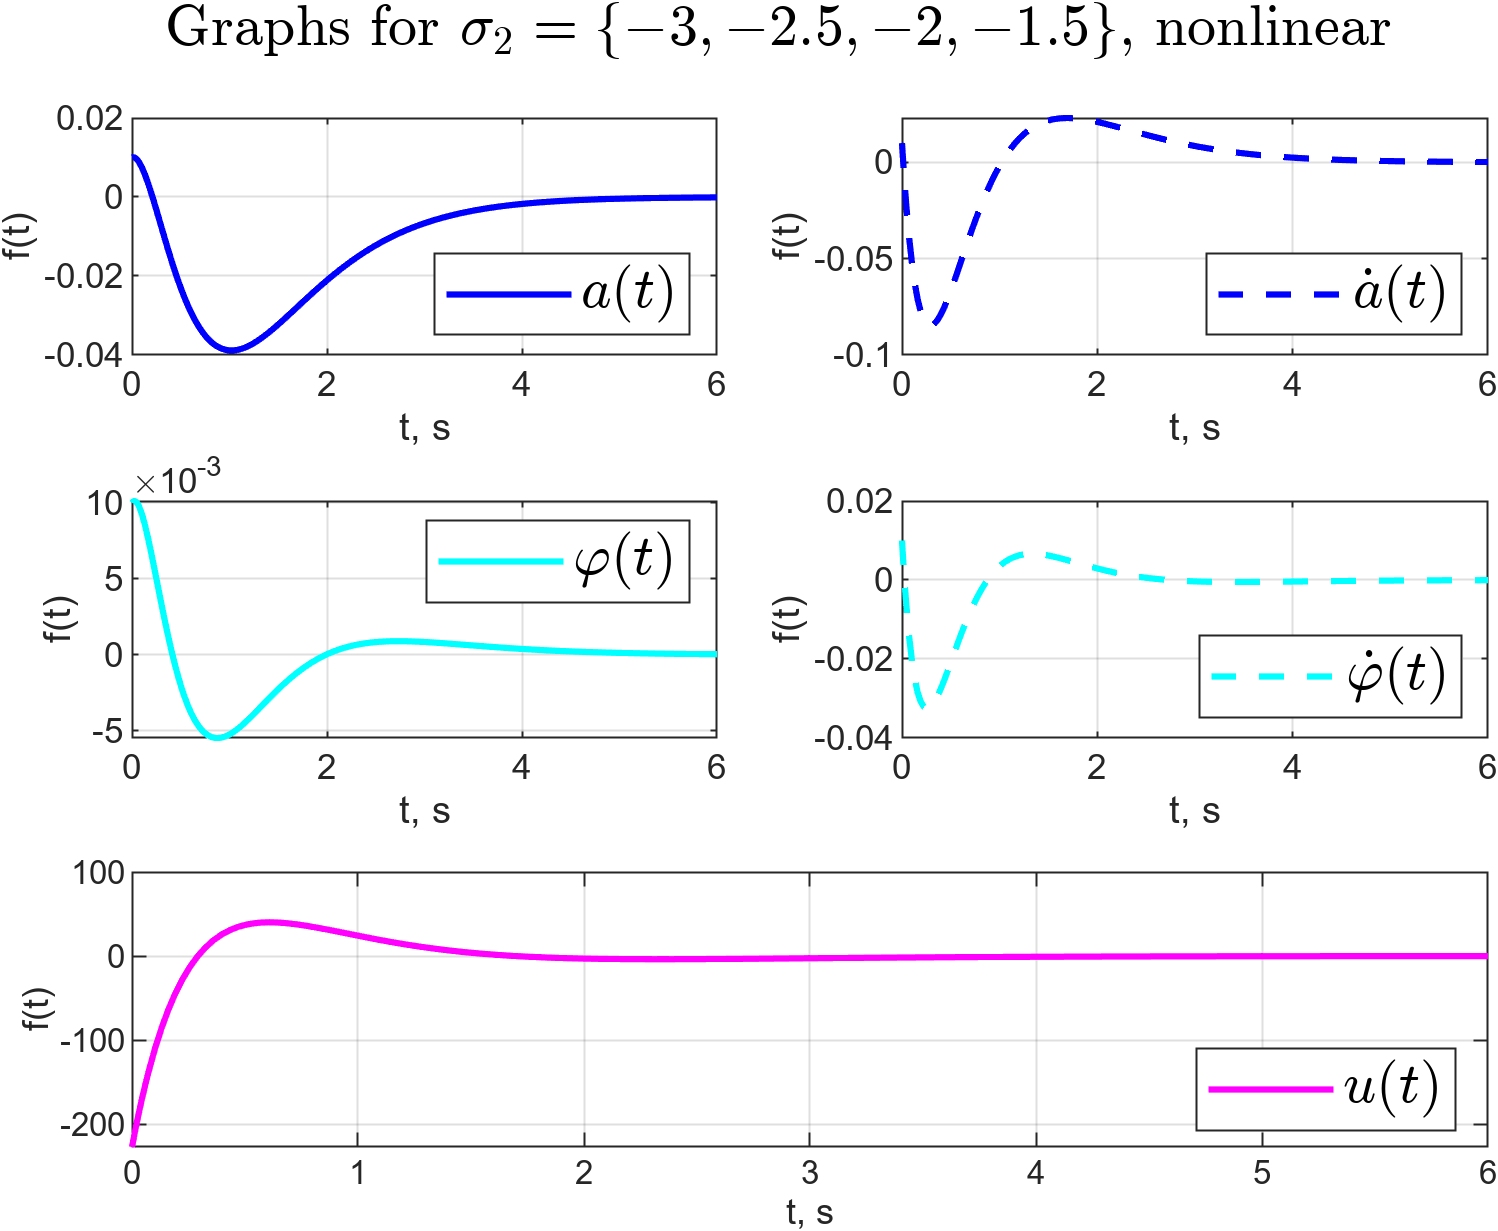
\includegraphics[width=1\linewidth]{pic/3_x_nlin_s2.png}}
\caption{Графики компонент вектора состояния системы и $u(t)$ для $\sigma_2$.}
\label{3_x_nlin_s2}
\end{figure}

\begin{figure}[!h]
\center{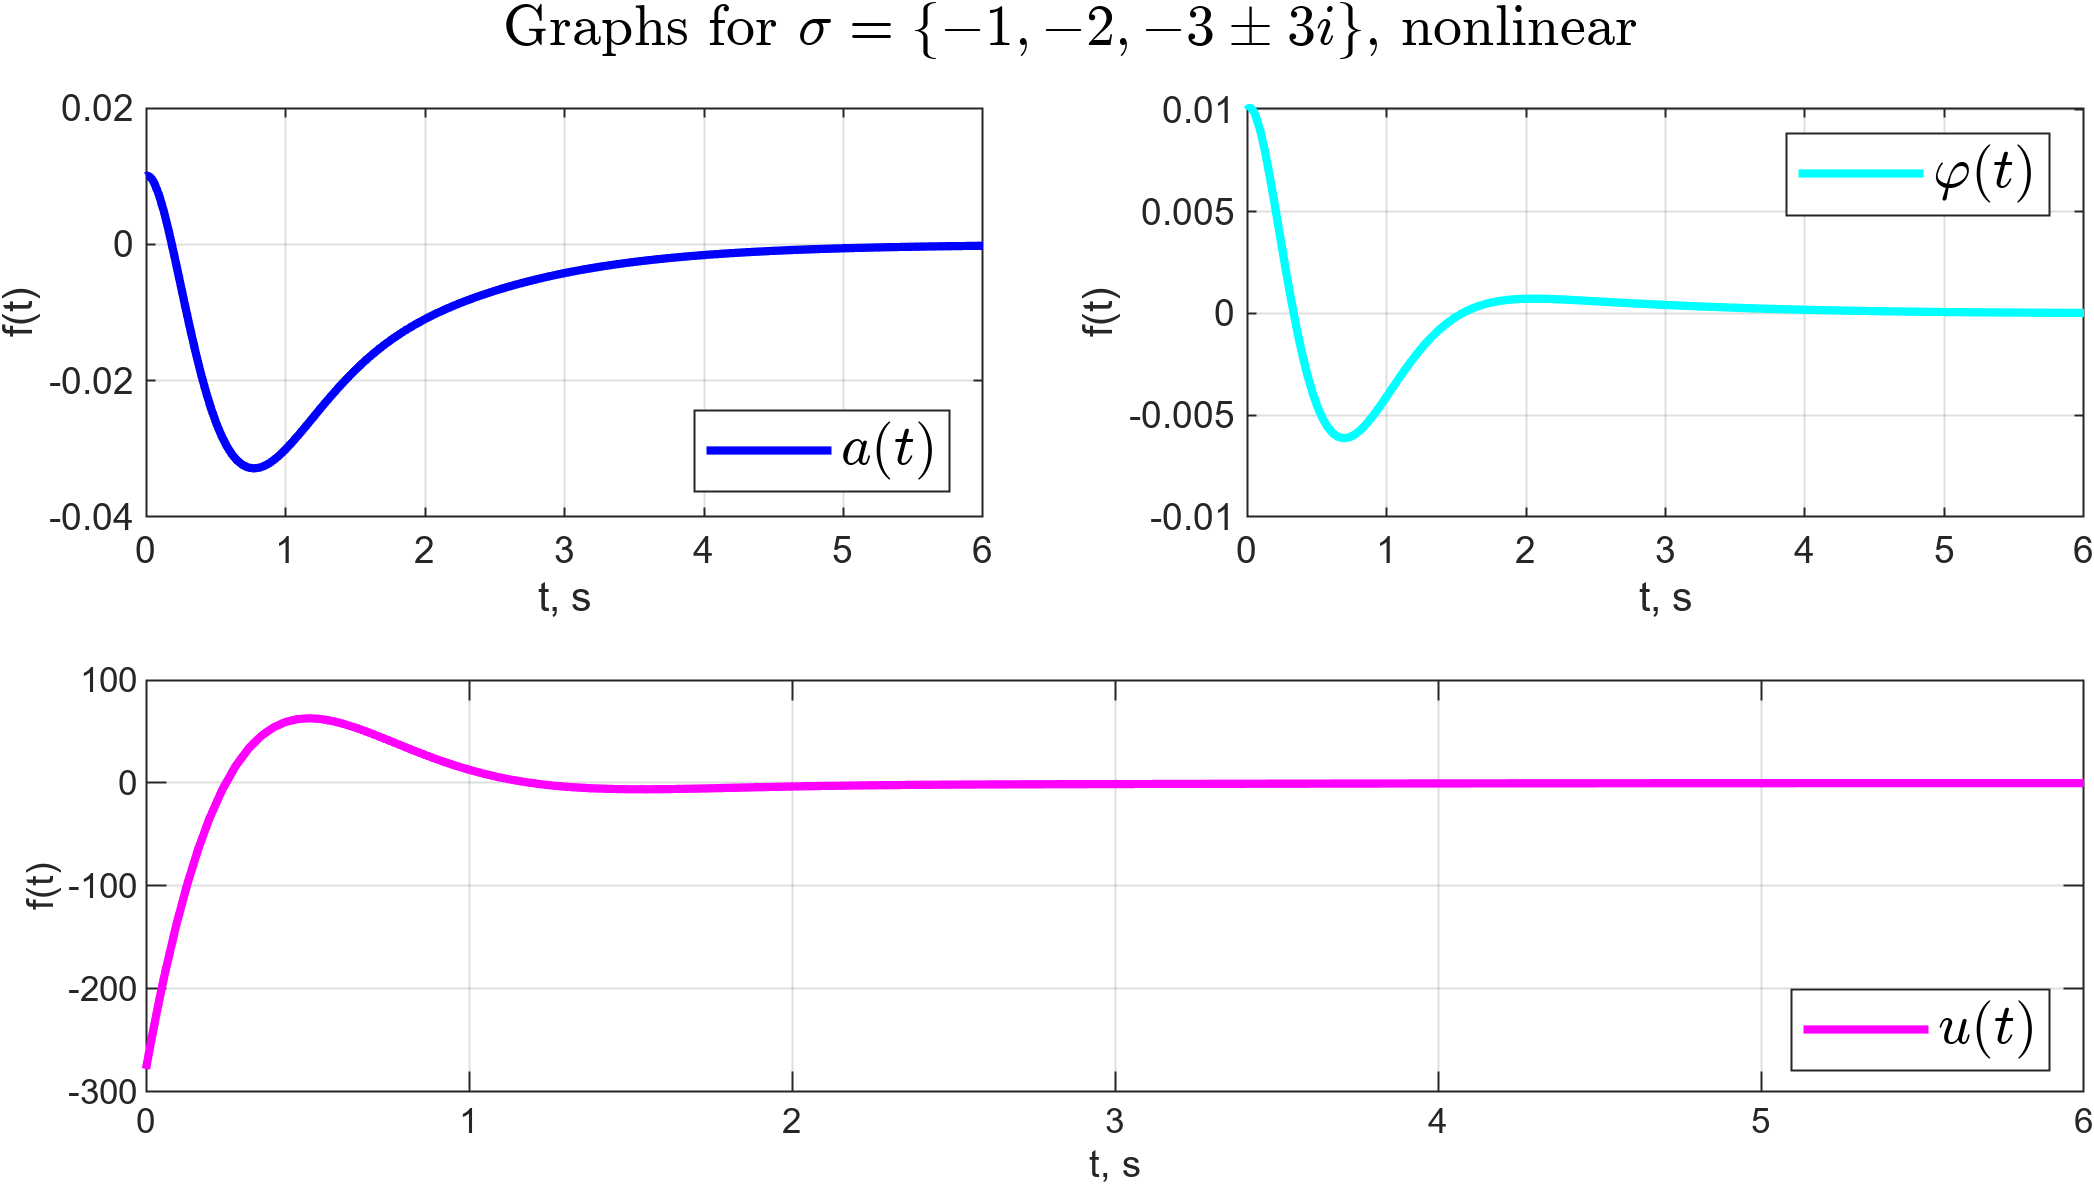
\includegraphics[width=1\linewidth]{pic/3_x_nlin_s3.png}}
\caption{Графики компонент вектора состояния системы и $u(t)$ для $\sigma_3$.}
\label{3_x_nlin_s3}
\end{figure}

\begin{figure}[!h]
\center{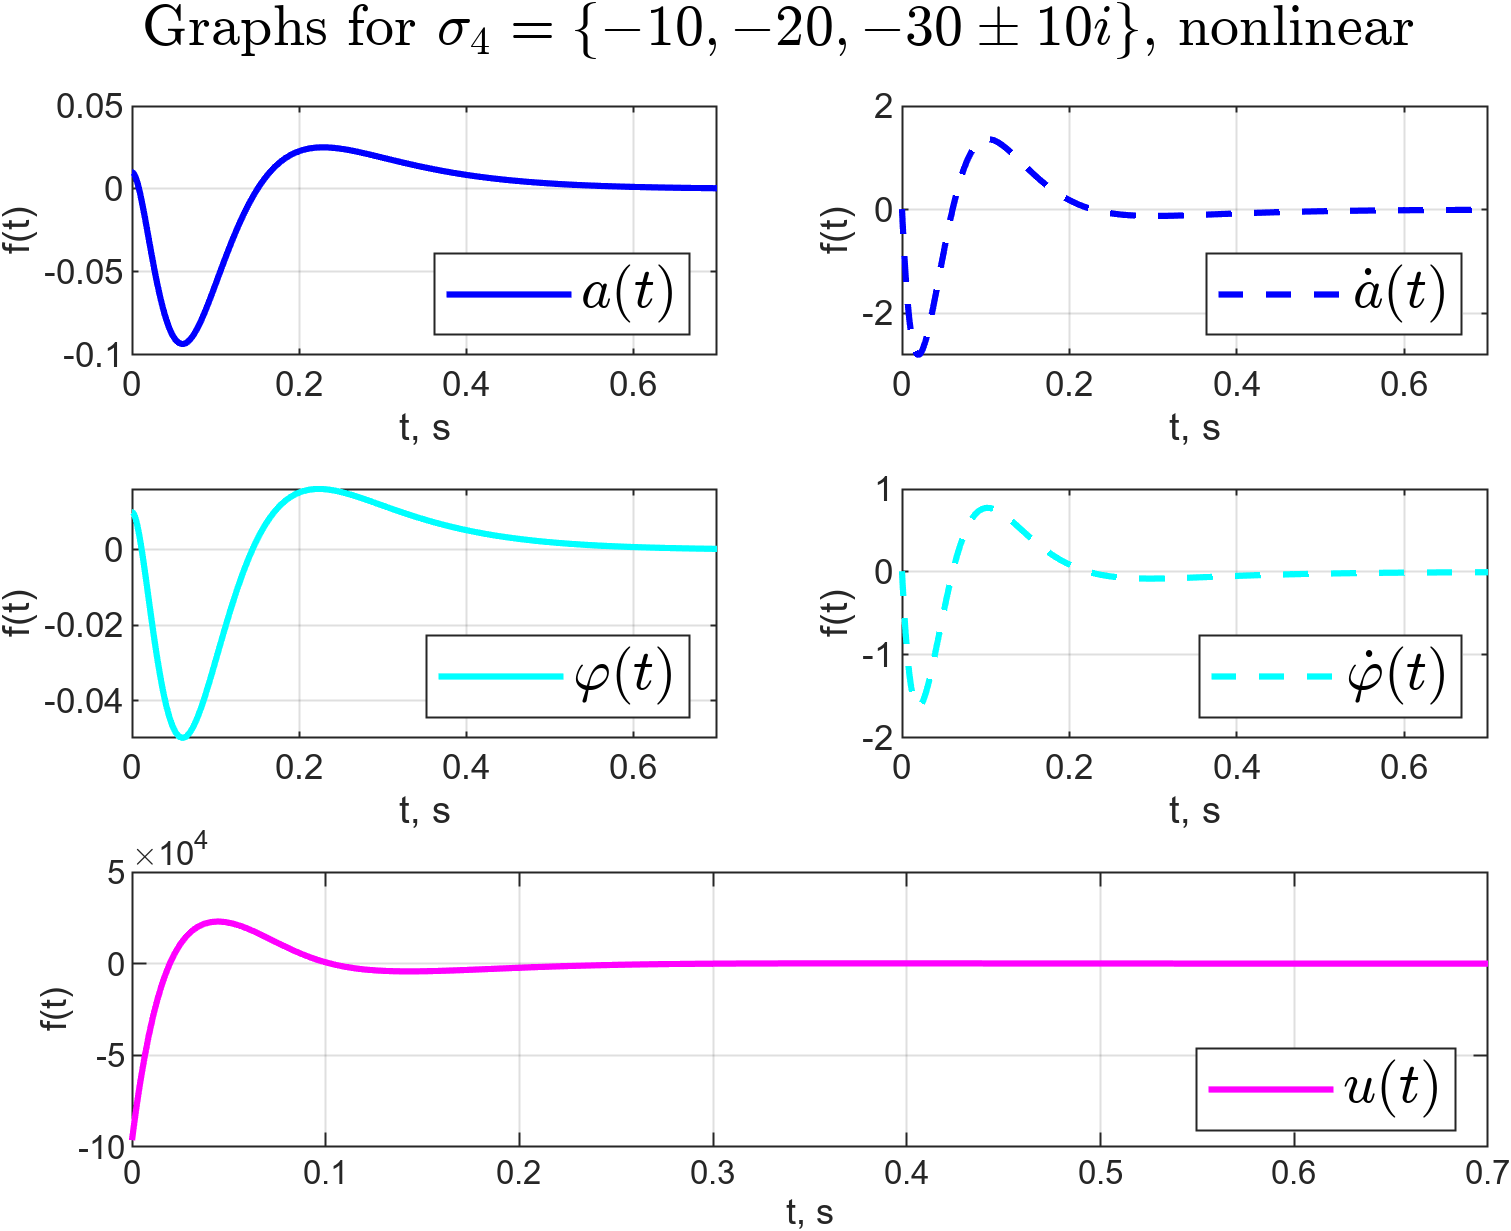
\includegraphics[width=1\linewidth]{pic/3_x_nlin_s4.png}}
\caption{Графики компонент вектора состояния системы и $u(t)$ для $\sigma_4$.}
\label{3_x_nlin_s4}
\end{figure}

Заметим, что при увеличении модулей значений спектра, возрастает максимальное значение управляющего сигнала, но уменьшается время, через которое вектор состояния системы становится неотличим от нуля. Результаты моделирования представлены на рисунках \ref{3_x_nlin_s1}-\ref{3_x_nlin_s4} (в данном задании для большей наглядности компоненты вектра состояния на графиках обозначены соответствующими физическими величинами).

\section{Синтез наблюдателя}

\subsection{Наблюдатель полной размерности}
Запишем наблюдатель полной размерности

\begin{equation}
    \begin{cases}
        \hat{y} = C \hat{x},\\
        \dot{\hat{x}} = A \hat{x} + Bu + L( \hat{y} - y)
    \end{cases}
\end{equation}


Для нахождения матрицы регулятора $L$ будем решать систему, содержающую уравнение Сильвестра

\begin{equation}
    \label{3_sil_obs}
    \begin{cases}
        \Gamma Q - Q A = YC\\
        L = Q^{-1}Y
    \end{cases}
\end{equation}
Запишем условия существования решения $Q$: $\sigma(A) \cap \sigma(\Gamma) = \emptyset$, $(\Gamma,Y)$ -- управляема, $(C, A)$ -- наблюдаема. Заметим, что последнее условие выполнено. 

Зададимся спектром $\sigma = \{ -1, -2, -3, -4  \}$, запишем подходящие матрицы $\Gamma$ и $Y$

\begin{equation}
\Gamma=
    \begin{bmatrix}
    -1	&0	&0	&0\\
0	&-2	&0	&0\\
0	&0&	-3	&0\\
0	&0	&0	&-4
\end{bmatrix}, \, \, 
Y  = \begin{bmatrix}
    1 & 1\\
    1 & 1\\
    1 & 1\\
    1 & 1
\end{bmatrix}
\end{equation}

Убедимся, что условие $(\Gamma,Y)$ -- управляема выполнено, составим матрицу управляемости и найдем ее ранг

\begin{multline}
    U = \begin{bmatrix}
    Y & \Gamma Y & \Gamma^2 Y &\Gamma^3 Y &
    \end{bmatrix} = \begin{bmatrix}
        1	&1&	-1&	-1&	1	&1&	-1&	-1\\
1	&1	&-2	&-2&	4&	4	&-8&	-8\\
1	&1	&-3&	-3&	9	&9	&-27&	-27\\
1	&1	&-4&	-4&	16&	16&	-64&	-64
    \end{bmatrix} \Rightarrow\\
    \Rightarrow rank(U) = 4
\end{multline}

Ранг матрицы $U$ равен размерности системы, $(\Gamma,Y)$ -- управляема.

Решим систему (\ref{3_sil_obs}) и получим $L$

\begin{equation}
    L = \begin{bmatrix}
        7.7918	&7.7918\\
2.2438	&2.2438\\
-17.7918	&-17.7918\\
-43.0833	&-43.0833
    \end{bmatrix}
\end{equation}

Выберем систему, замкнутую систему со спектром $\sigma_2 = \{ -3, -2.5, -2, -1.5 \}$ из исследованных ранее в пункте 3.2.


Запишем начальные условия системы и наблюдателя

\begin{equation}
    \begin{matrix}
        x(0) = \begin{bmatrix}
    0.01&&
    0.01&&
    0.01&&
    0.01
\end{bmatrix}^T\\
 \hat{x}(0) = \begin{bmatrix}
    0&&
    0&&
    0&&
    0
\end{bmatrix}^T
    \end{matrix}
\end{equation}

Построим графики $x(t)$ и $\hat{x}$ (рисунок \ref{3_xx_nlin_02_L1}) и график ошибки $e(t) = \hat{x}(t) - x(t)$ (рисунок \ref{3_e_nlin_02_L1}). Заметим, что синтезированный наблюдатель работает довольно успешно: ошибка наблюдения становится визуально неотличима от нуля после $t=2$ с.

\begin{figure}[!h]
\center{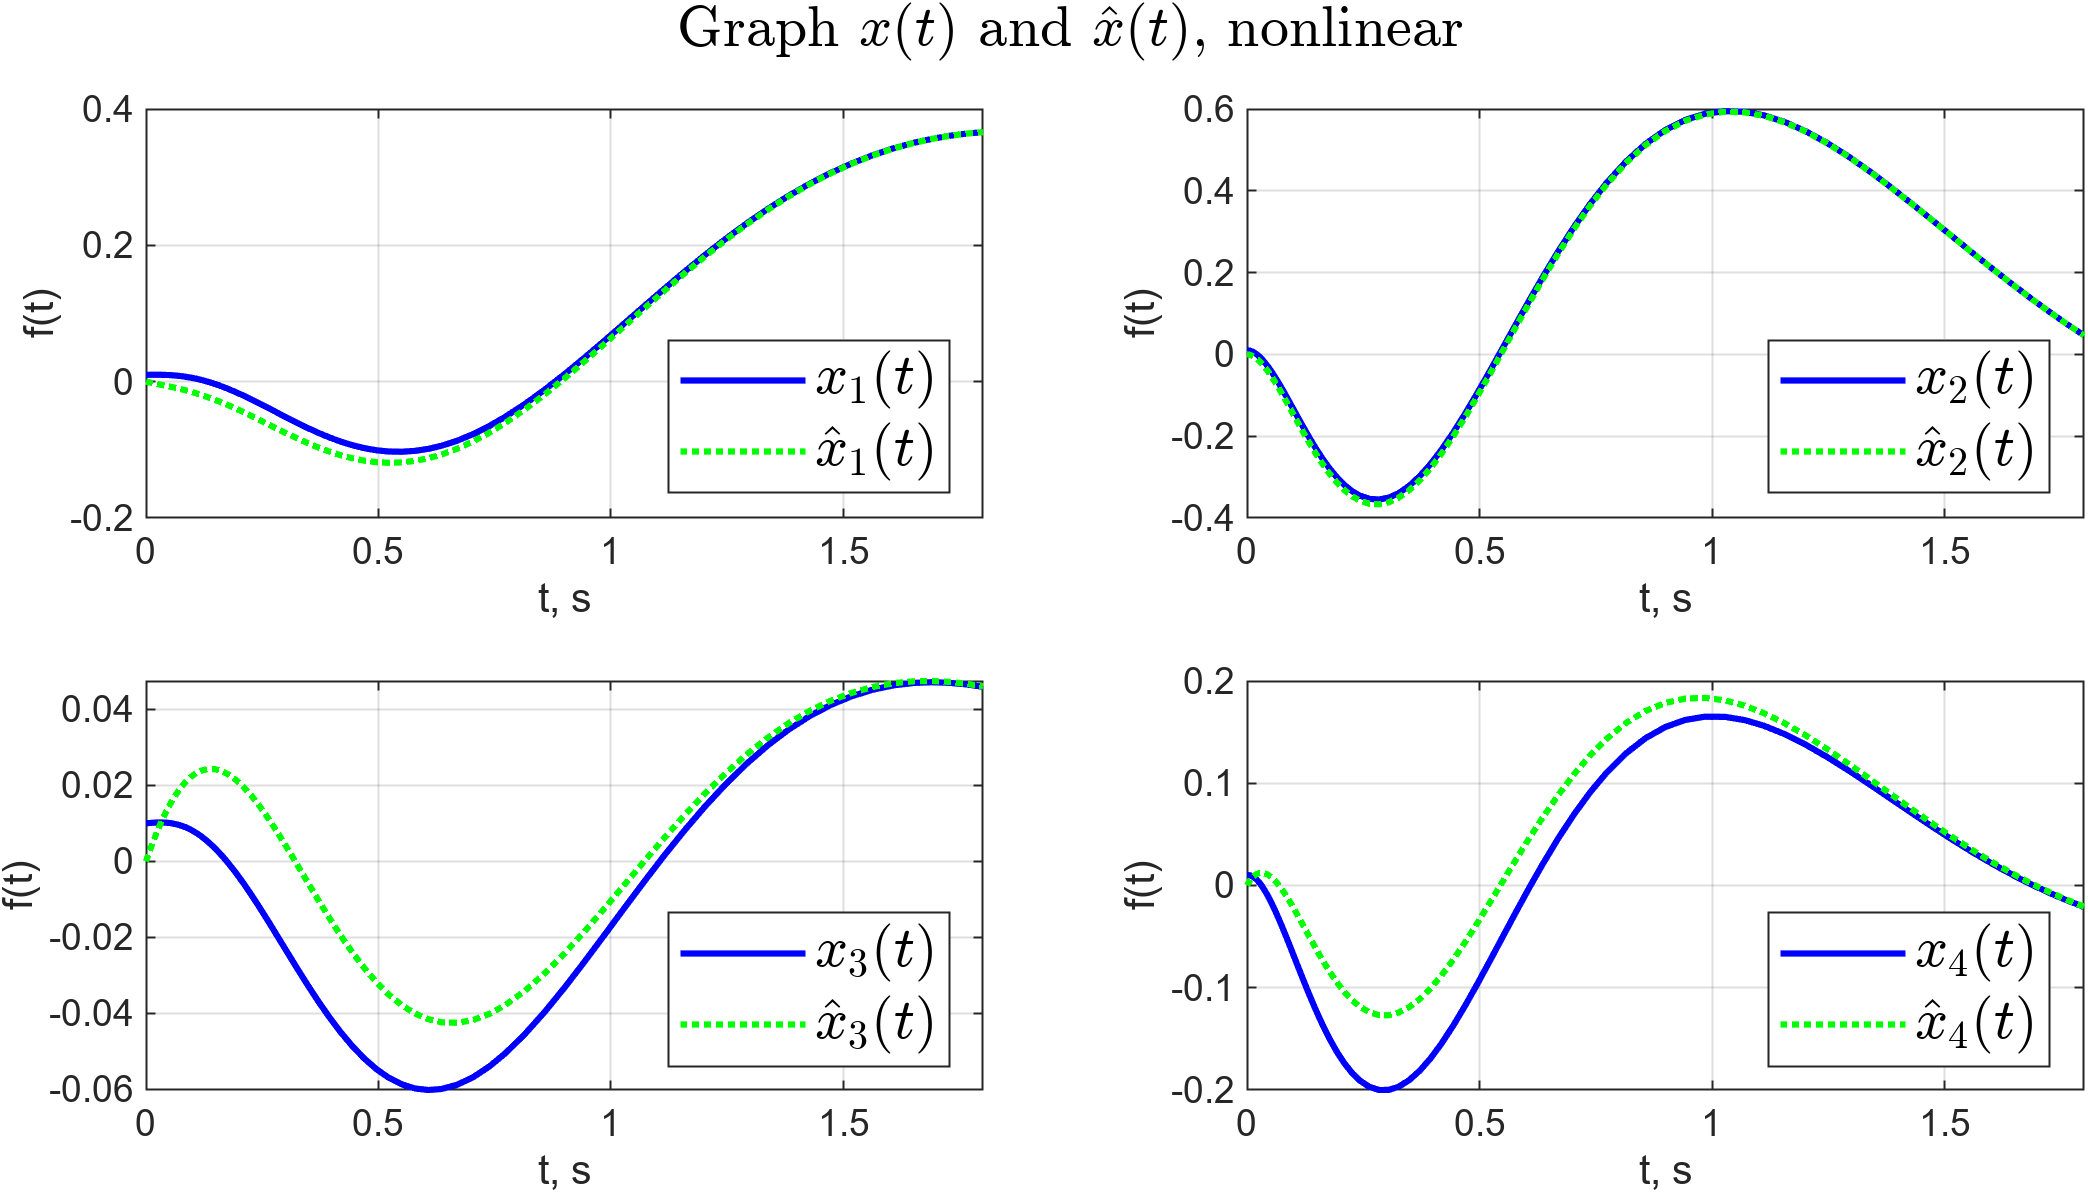
\includegraphics[width=1\linewidth]{pic/3_xx_nlin_02_L1.png}}
\caption{Графики $x(t)$ и $\hat{x}(t)$.}
\label{3_xx_nlin_02_L1}
\end{figure}


\begin{figure}[!h]
\center{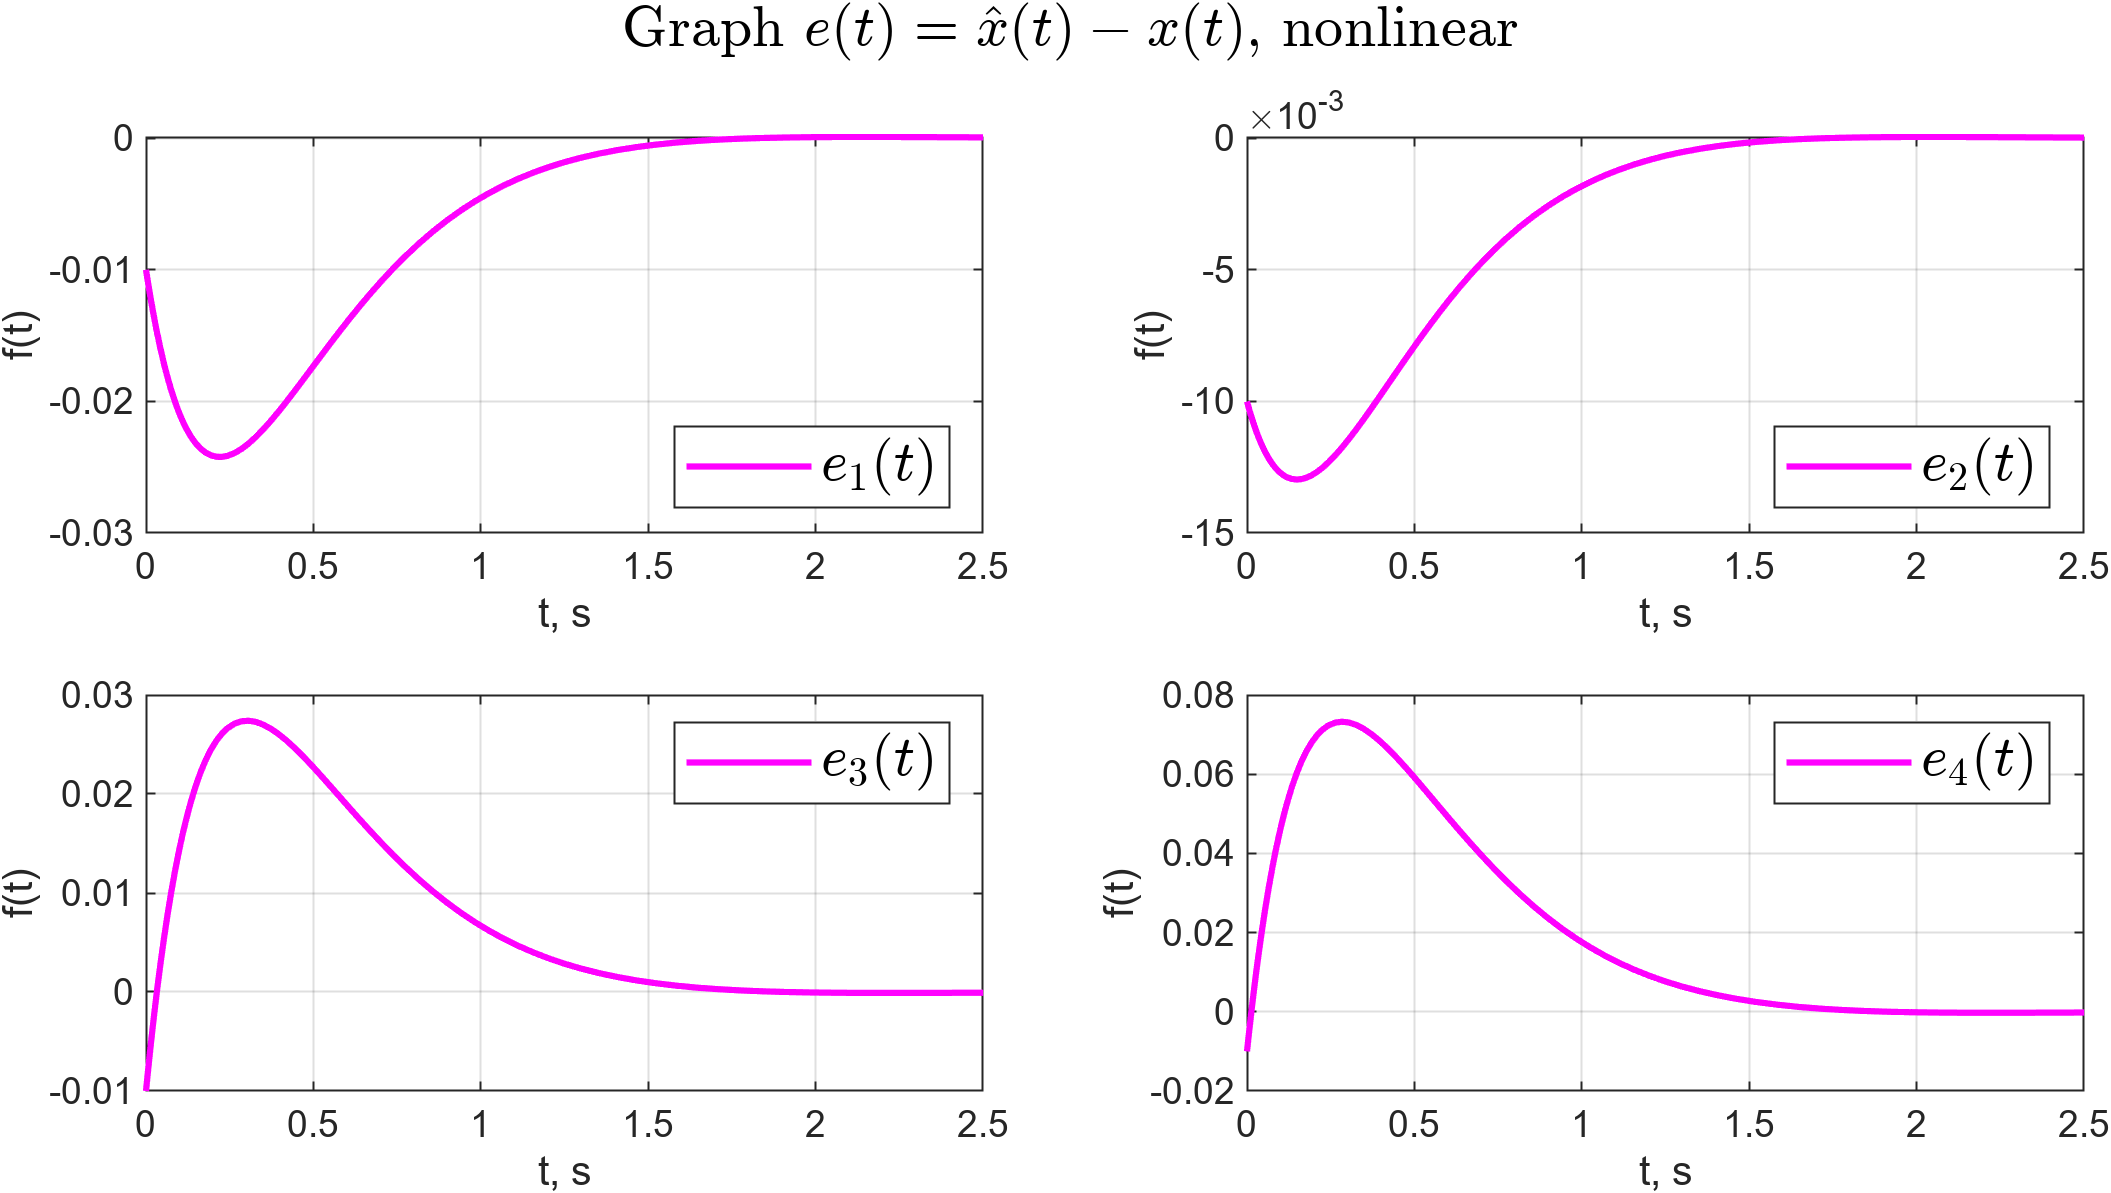
\includegraphics[width=1\linewidth]{pic/3_e_nlin_02_L1.png}}
\caption{Графики $e (t) =\hat{x}(t) - x(t)$.}
\label{3_e_nlin_02_L1}
\end{figure}

Теперь зададимся несколькими дополнительными наборами собственных чисел наблюдателя и исследуем их влияние на систему

\begin{equation*}
  \begin{matrix}
      \sigma_1 = \{ -0.1, -0.2, -0.3, -0.4 \}, & \sigma_2 = \{ -5, -10, -15, -20 \},\\
      \sigma_3 = \{ -1, -2, -3 \pm 3i \} & 
 \end{matrix}
\end{equation*}

\begin{figure}[!h]
\center{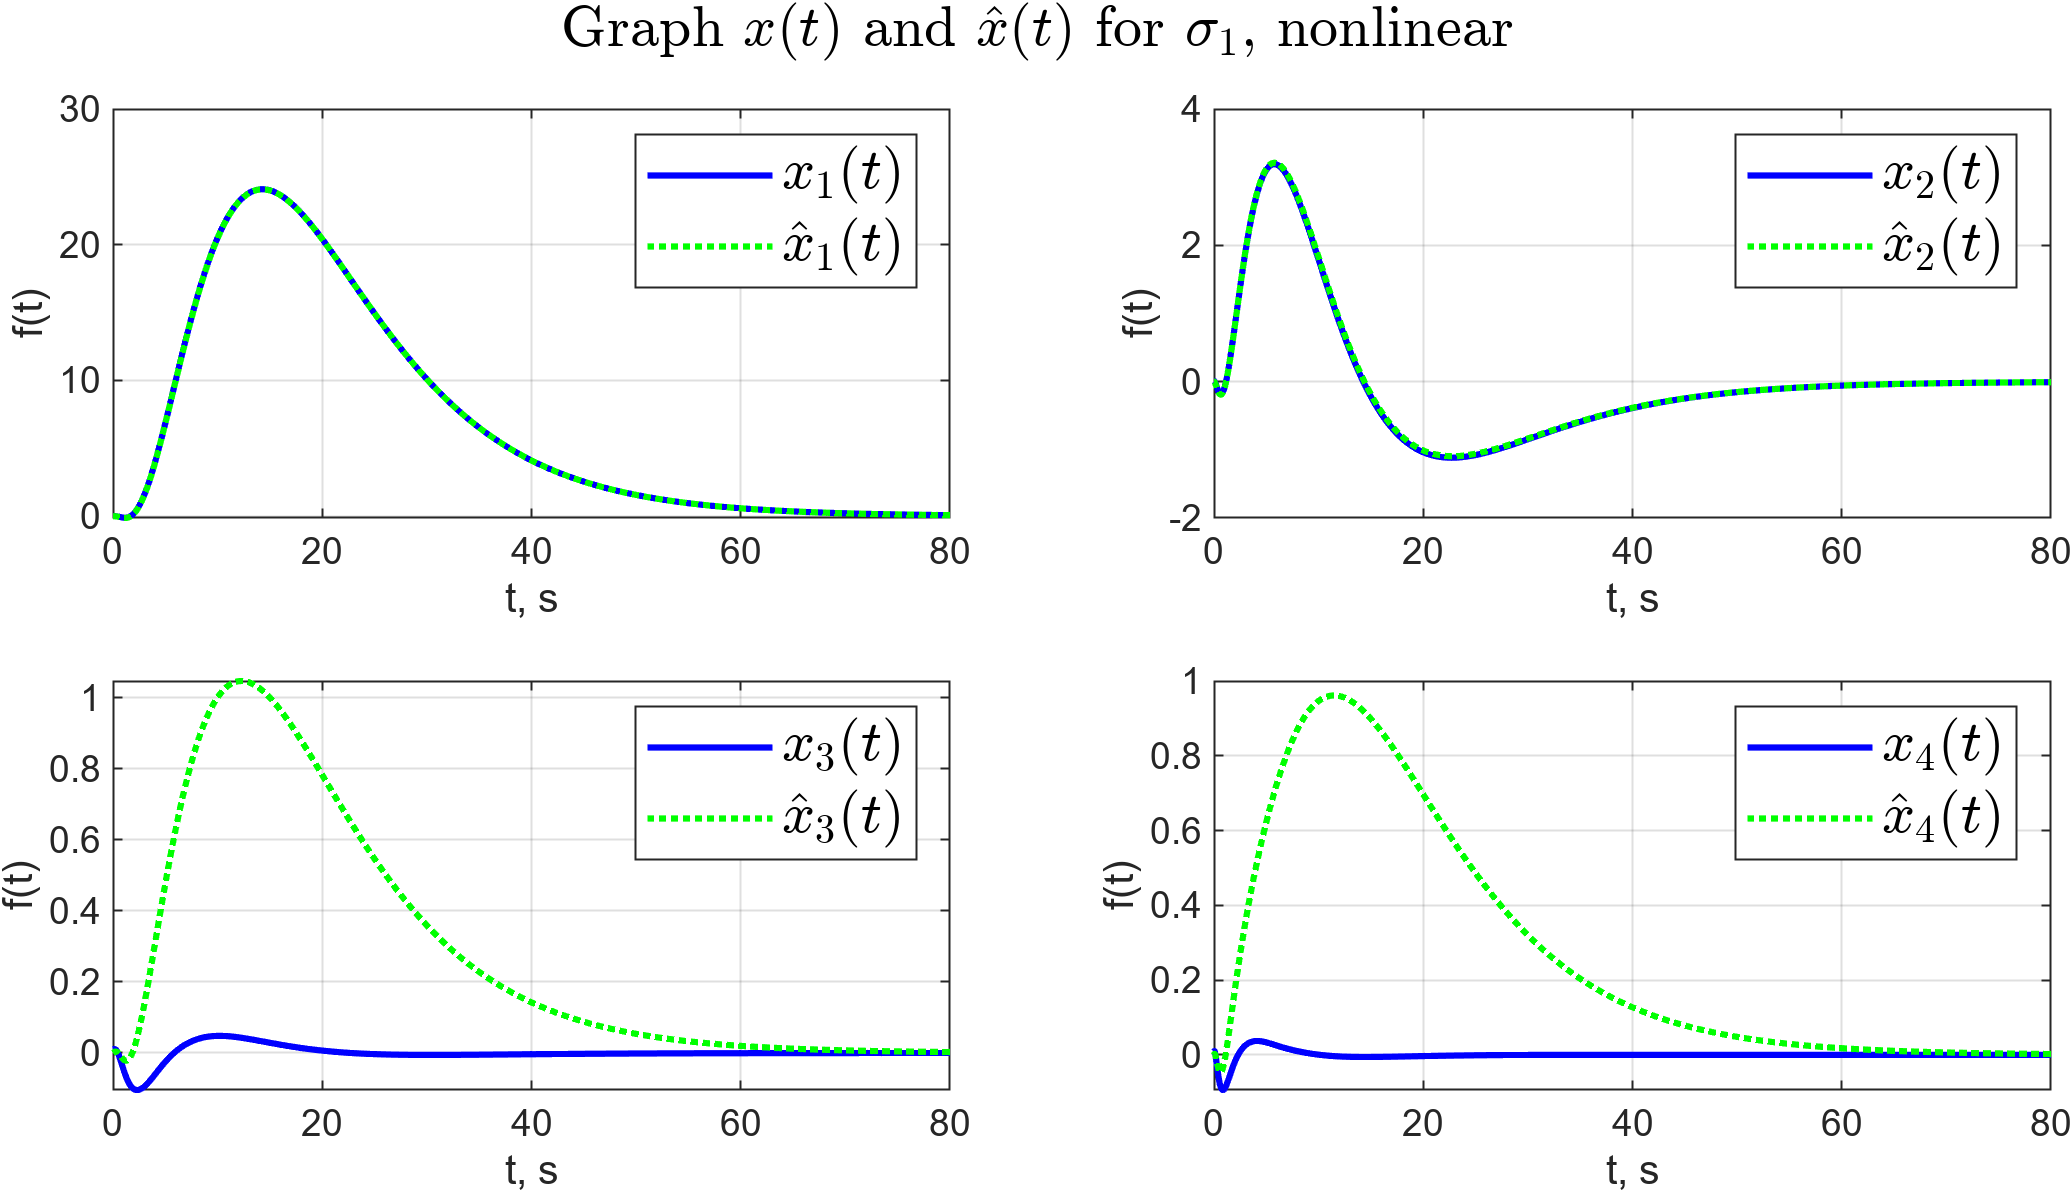
\includegraphics[width=1\linewidth]{pic/3_xx_nlin_02_L2.png}}
\caption{Графики $x(t)$ и $\hat{x}(t)$ для $ \sigma_1 = \{ -0.1, -0.2, -0.3, -0.4 \}$.}
\label{3_xx_nlin_02_L2}
\end{figure}


\begin{figure}[!h]
\center{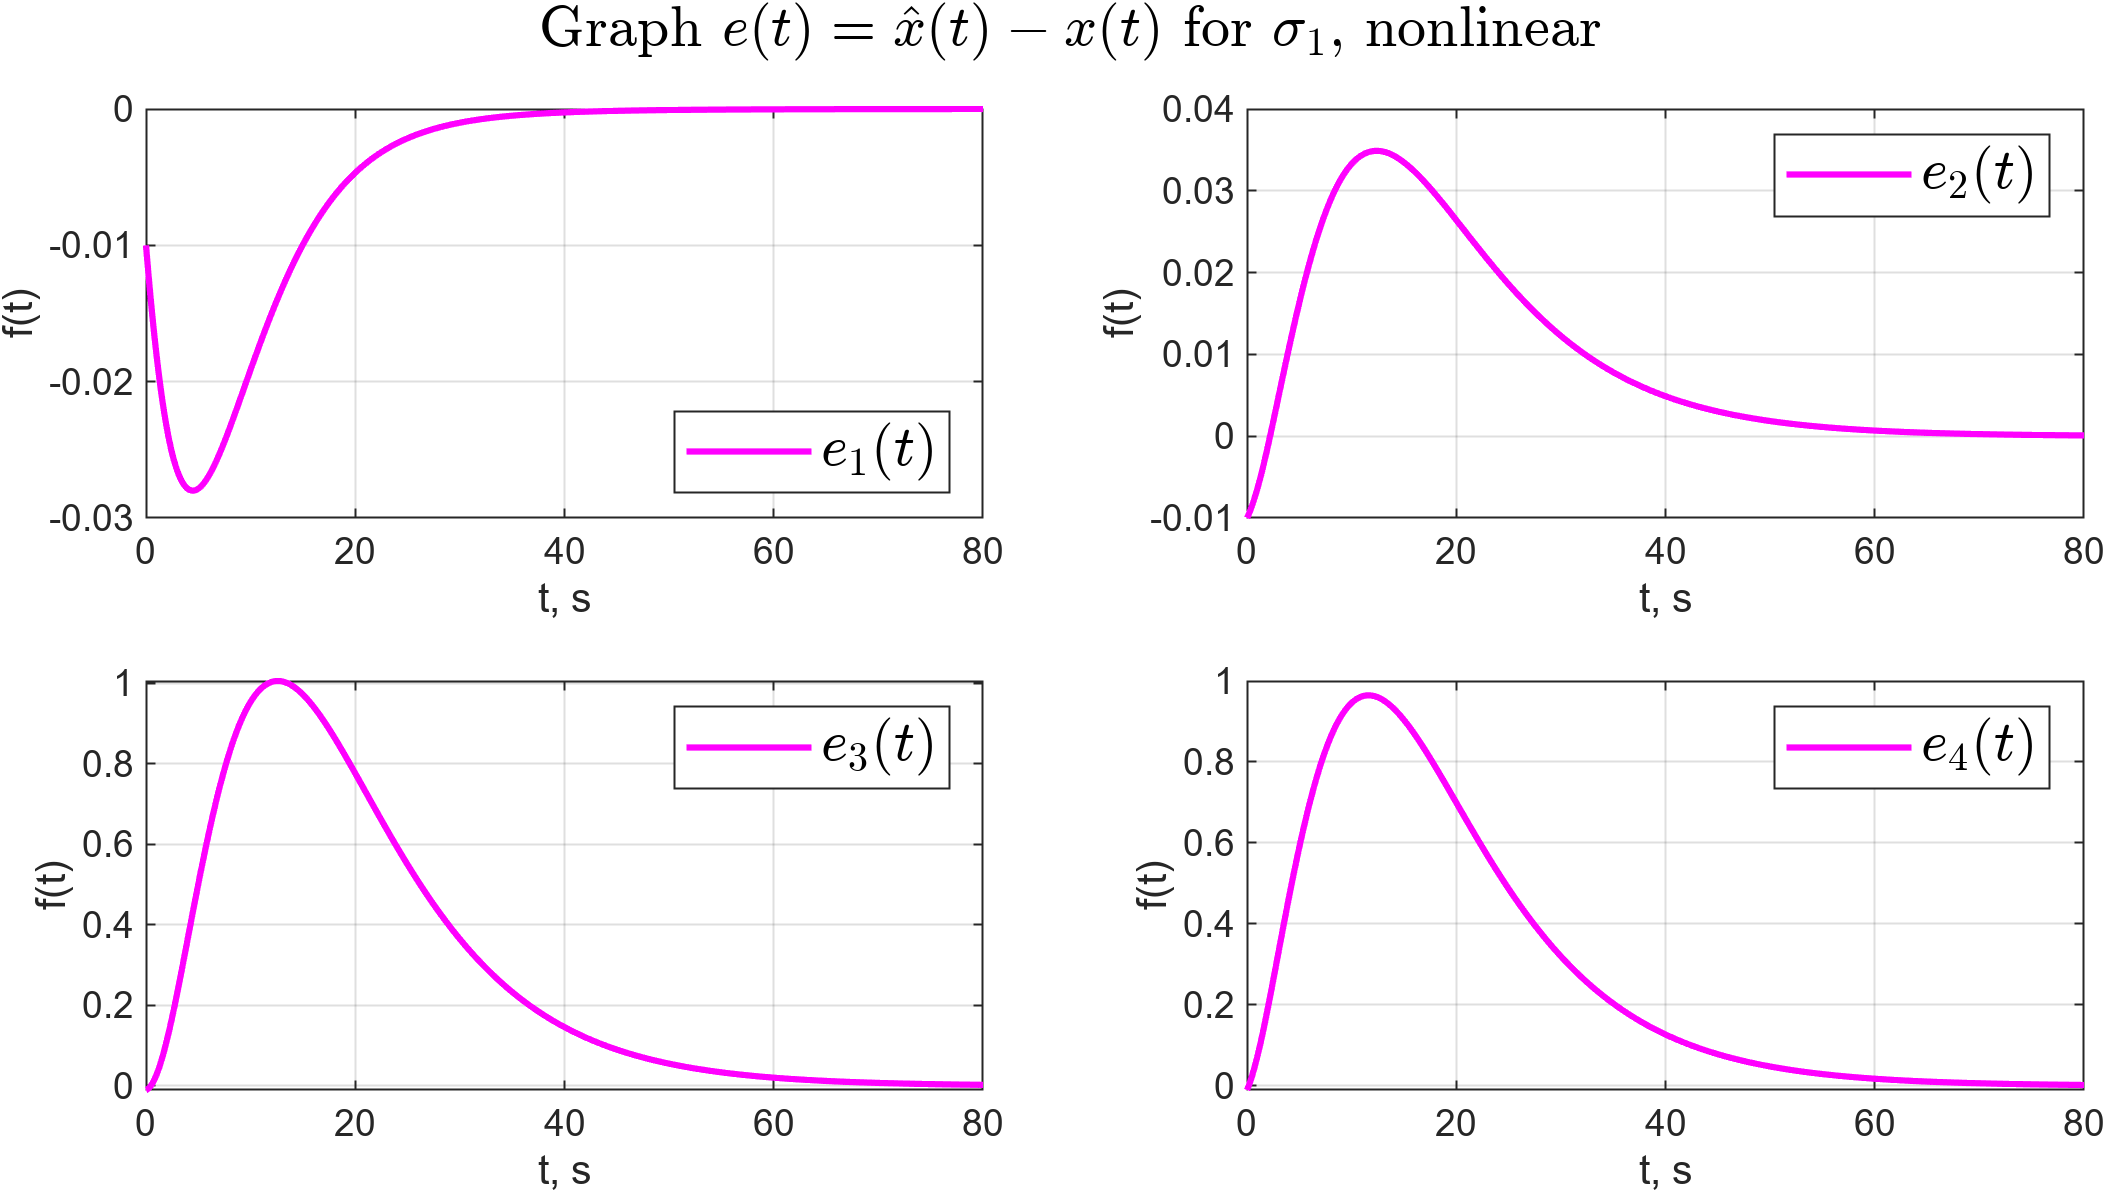
\includegraphics[width=1\linewidth]{pic/3_e_nlin_02_L2.png}}
\caption{Графики $e (t) =\hat{x}(t) - x(t)$ для $ \sigma_1 = \{ -0.1, -0.2, -0.3, -0.4 \}$.}
\label{3_e_nlin_02_L2}
\end{figure}

При малых значениях спектра наблюдателя  $ \sigma_1 = \{ -0.1, -0.2, -0.3, -0.4 \}$ наблюдатель выполняет свою задачу (рисунки \ref{3_xx_nlin_02_L2} и \ref{3_e_nlin_02_L2}), время, за которое ошибка наблюдения сходится к нулю сильно возрастает (до $\approx 80$ с).



\begin{figure}[!h]
\center{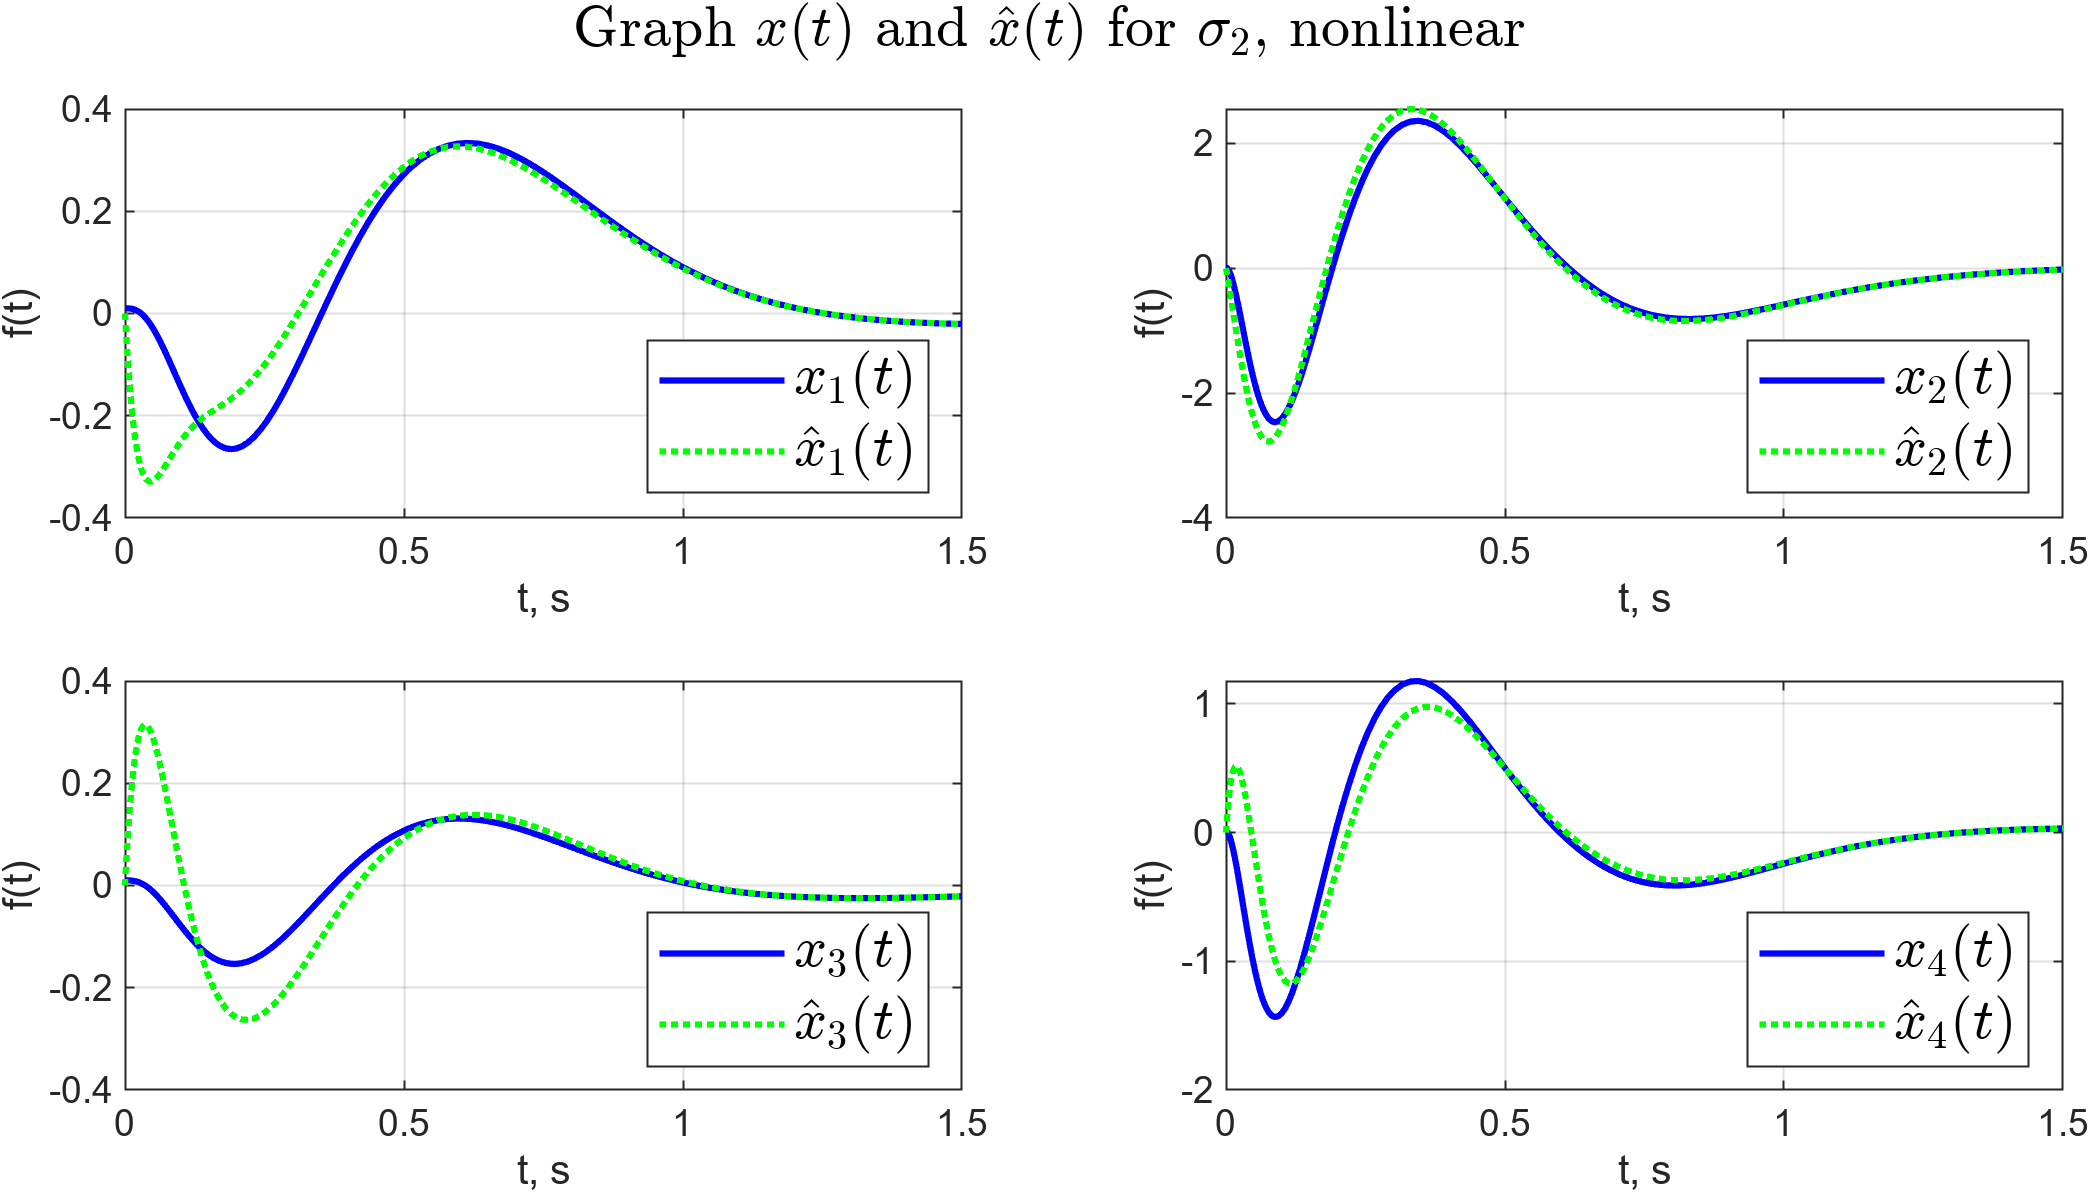
\includegraphics[width=1\linewidth]{pic/3_xx_nlin_02_L3.png}}
\caption{Графики $x(t)$ и $\hat{x}(t)$ для $ \sigma_2 = \{ -5, -10, -15, -20 \}$.}
\label{3_xx_nlin_02_L3}
\end{figure}


\begin{figure}[!h]
\center{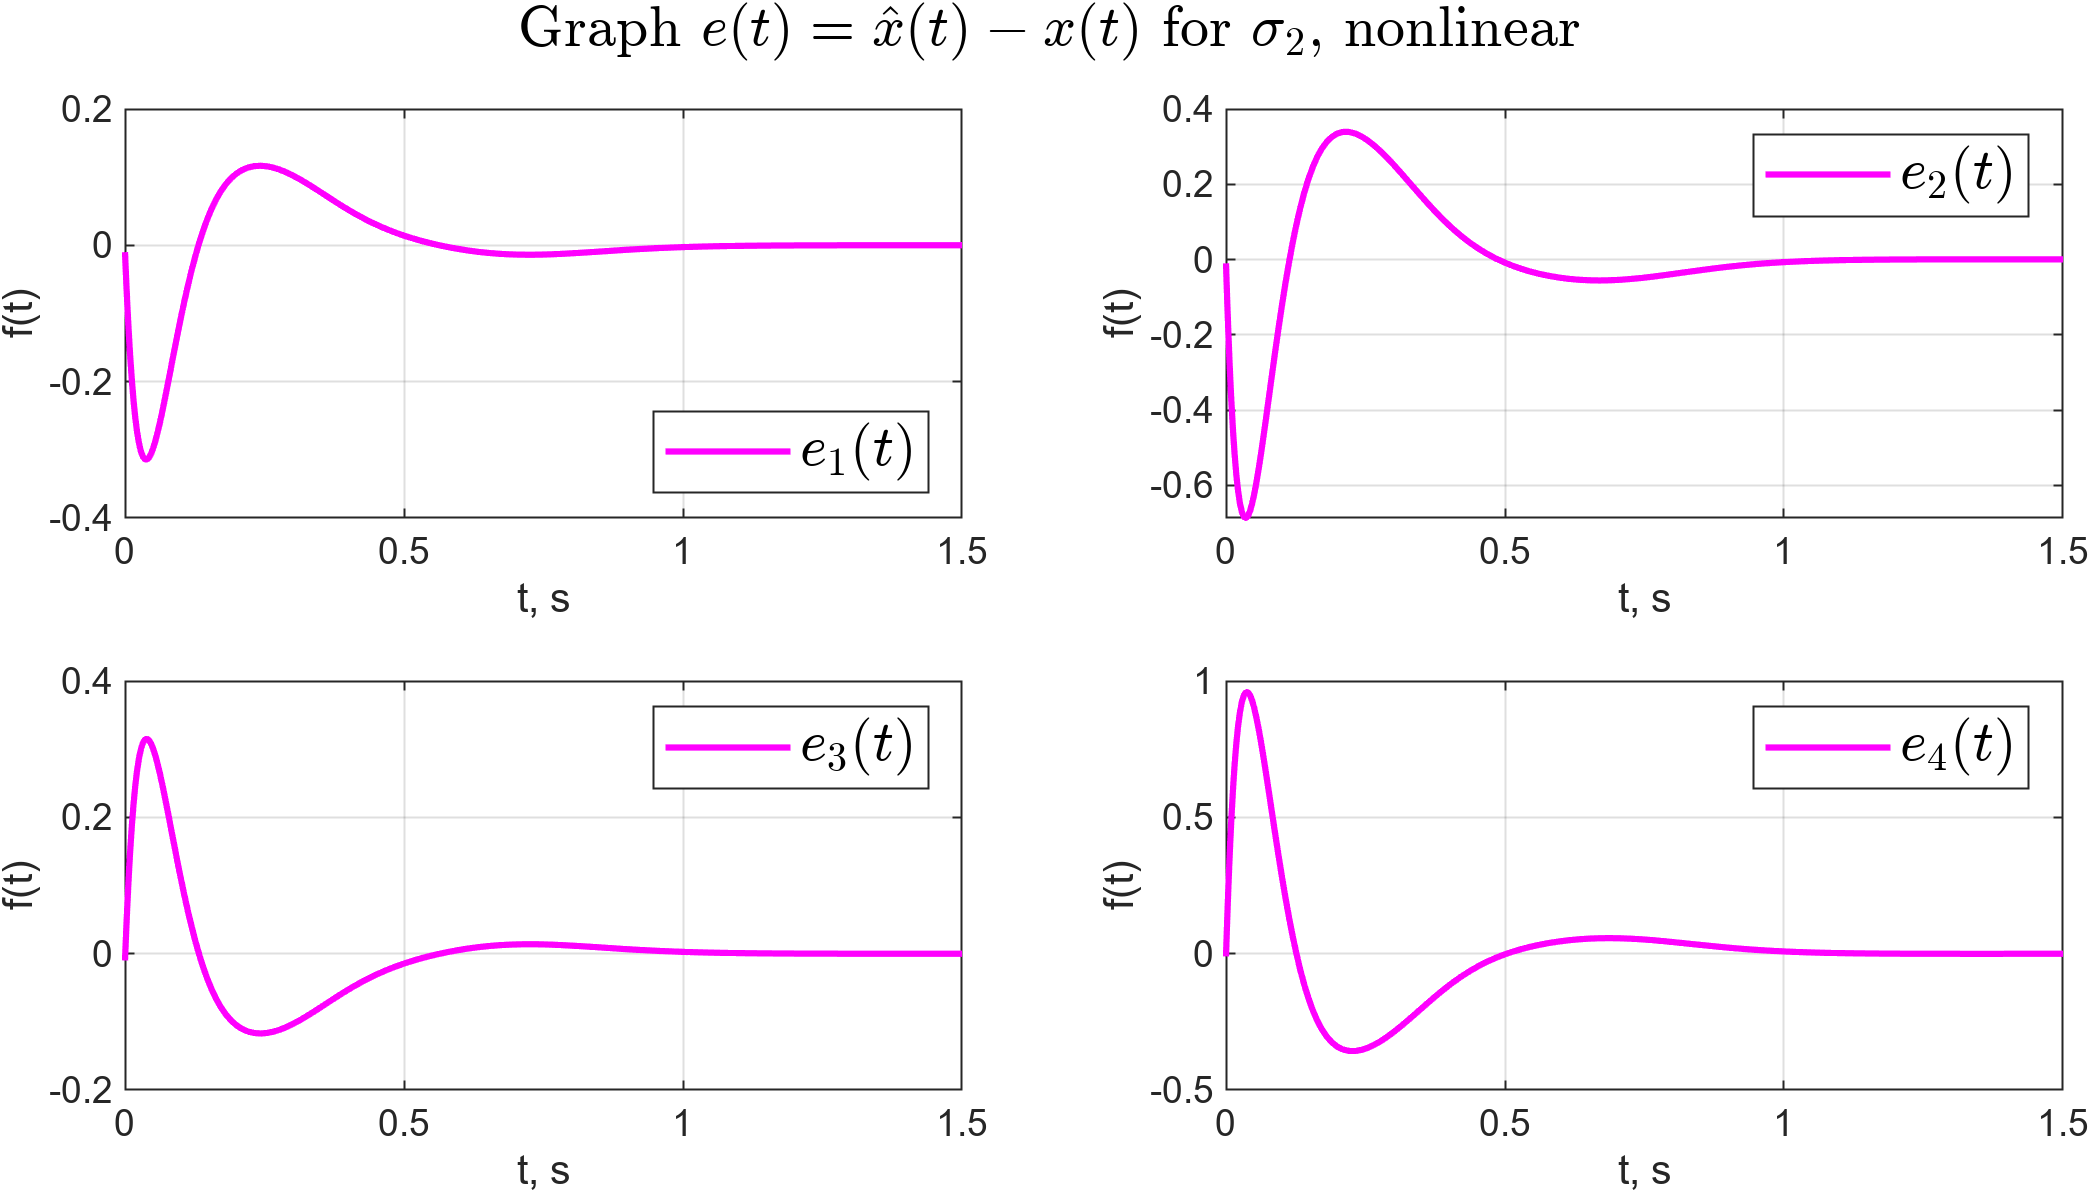
\includegraphics[width=1\linewidth]{pic/3_e_nlin_02_L3.png}}
\caption{Графики $e (t) =\hat{x}(t) - x(t)$ для $ \sigma_2 = \{ -5, -10, -15, -20 \}$.}
\label{3_e_nlin_02_L3}
\end{figure}

При больших значениях собственных чисел наблюдателя $ \sigma_1 = \{ -5, -10, -15, -20 \}$ время, после которого ошибка наблюдения становится неотличима от нуля, существенно сокращается до $\approx 1$ секунды. 

\begin{figure}[!h]
\center{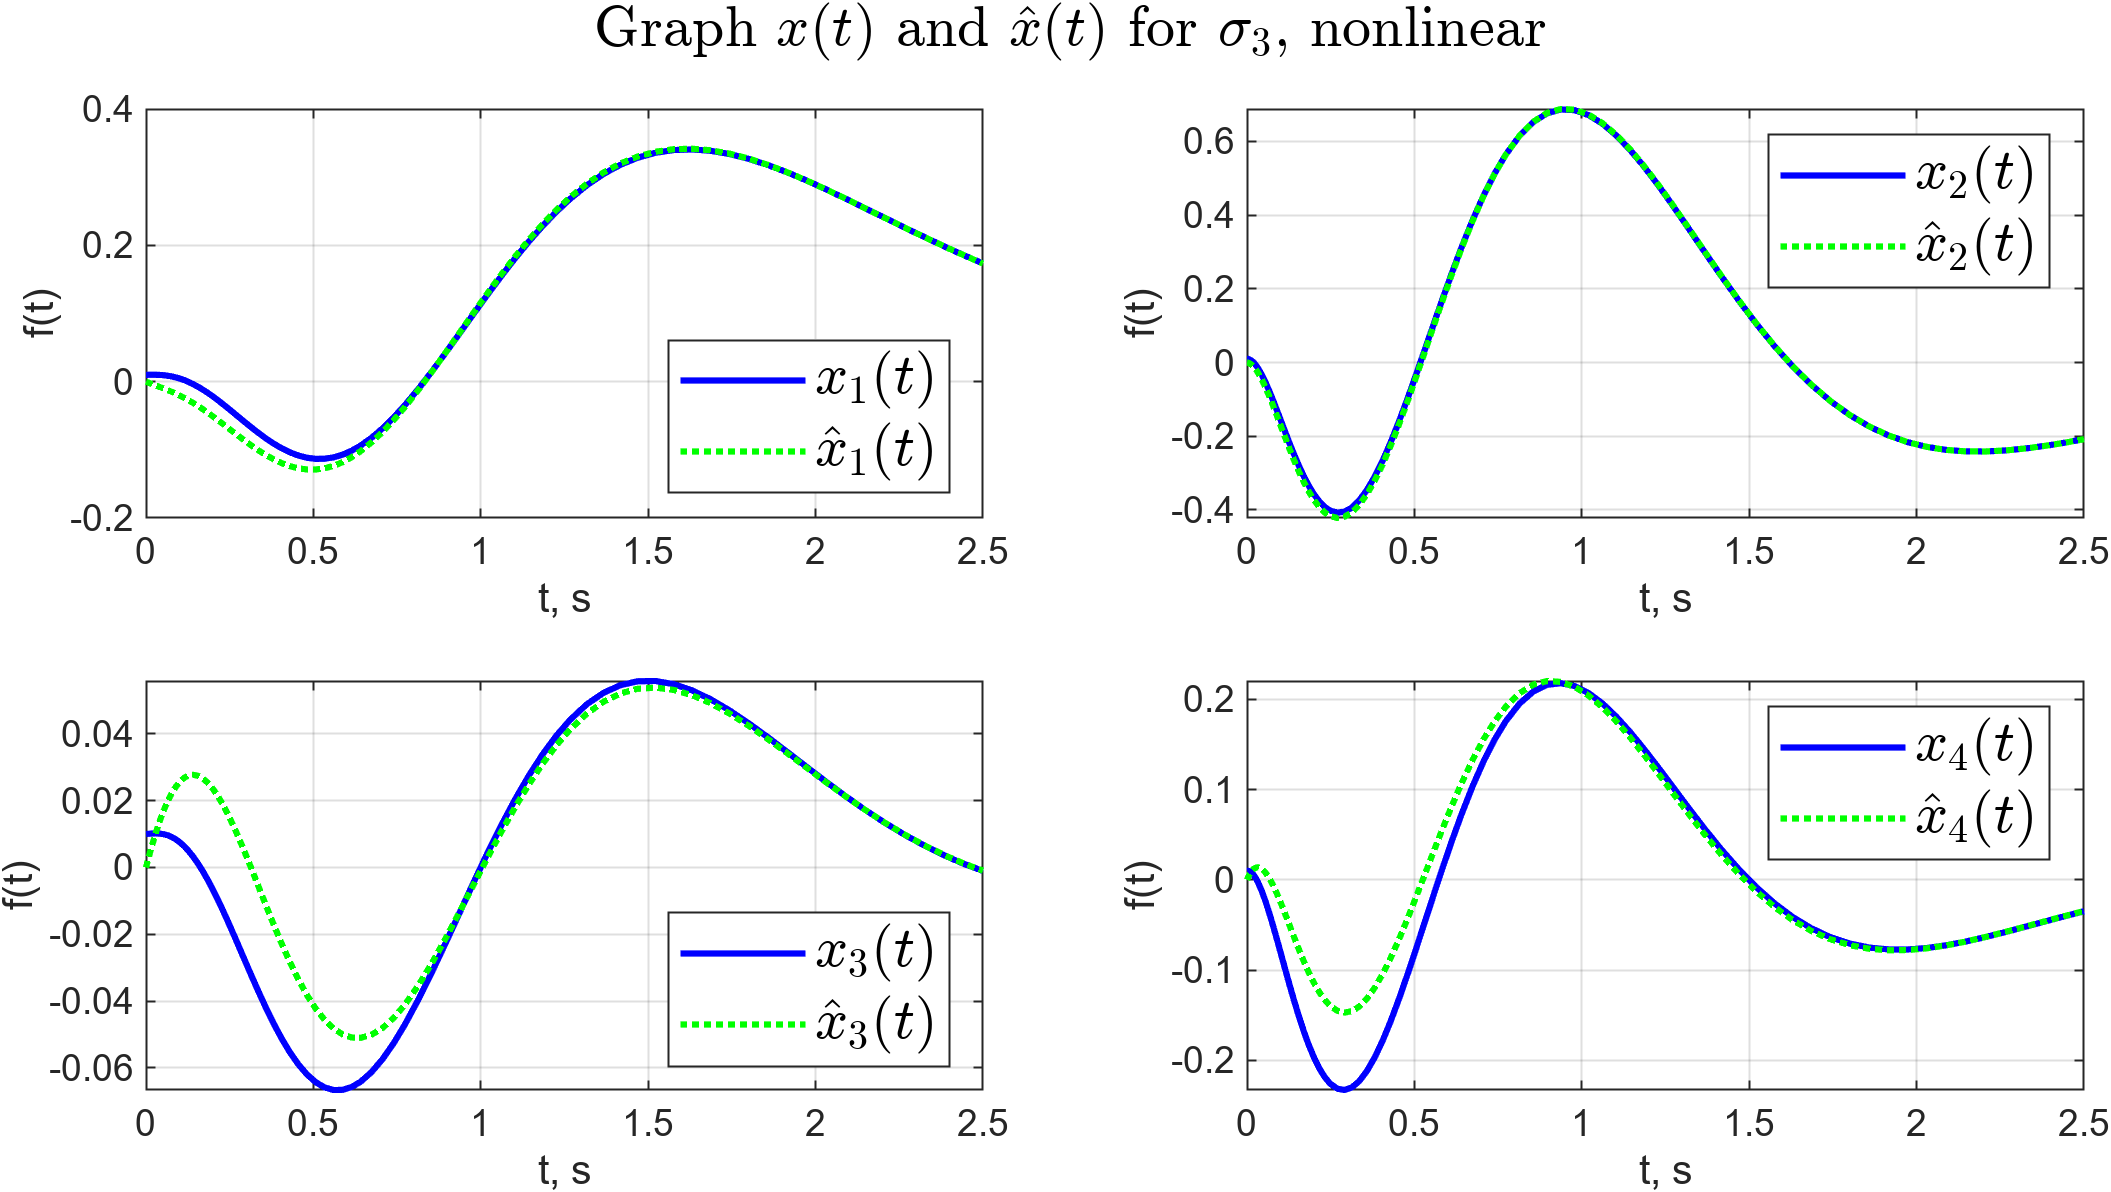
\includegraphics[width=1\linewidth]{pic/3_xx_nlin_02_L4.png}}
\caption{Графики $x(t)$ и $\hat{x}(t)$ для $ \sigma_3 = \{ -1, -2, -3 \pm 3i \}$.}
\label{3_xx_nlin_02_L4}
\end{figure}


\begin{figure}[!h]
\center{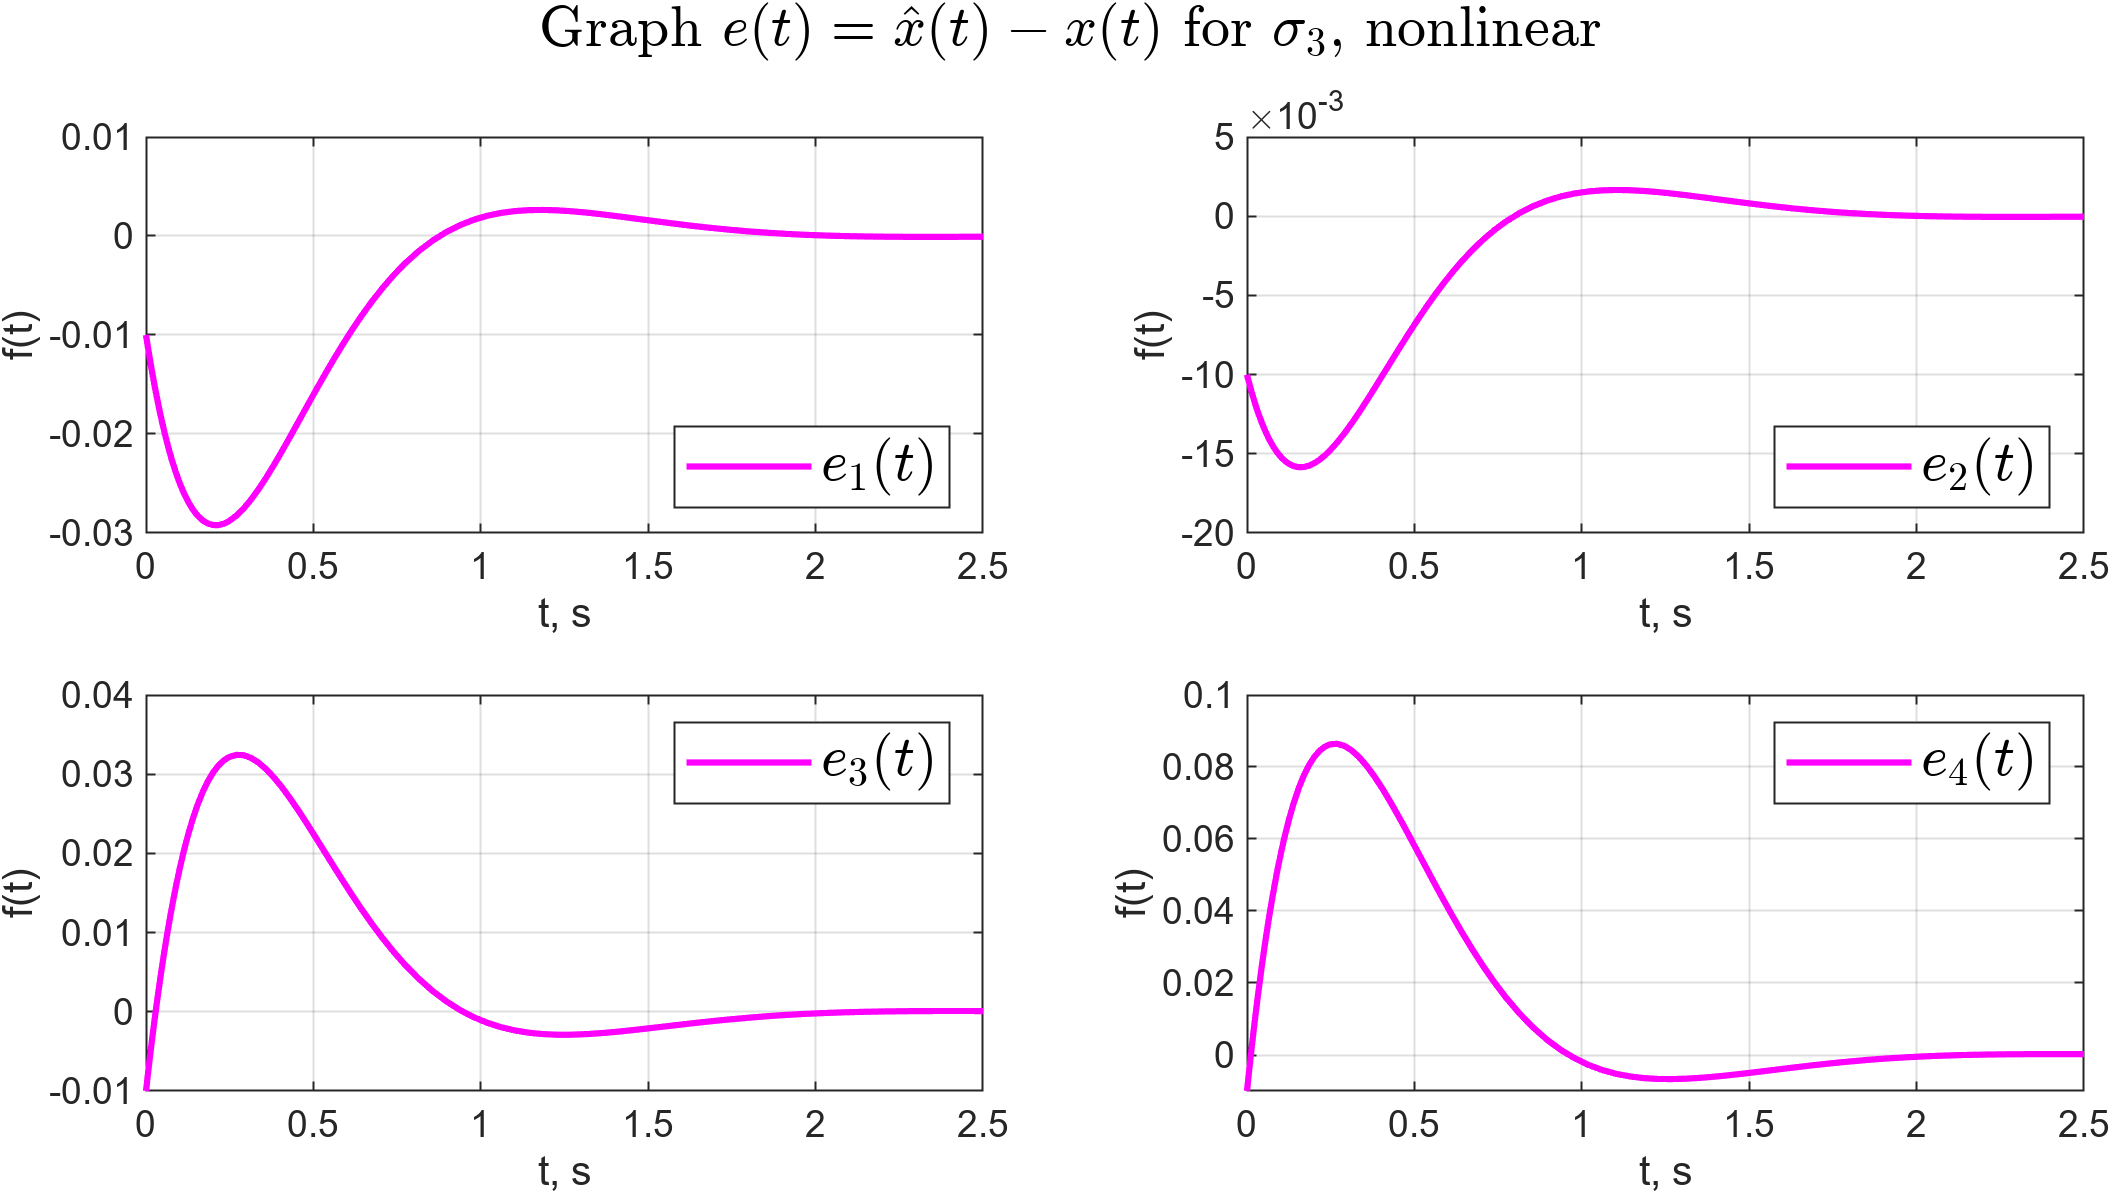
\includegraphics[width=1\linewidth]{pic/3_e_nlin_02_L4.png}}
\caption{Графики $e (t) =\hat{x}(t) - x(t)$ для $ \sigma_3 = \{ -1, -2, -3 \pm 3i \}$.}
\label{3_e_nlin_02_L4}
\end{figure}


\newpage
\subsection{Наблюдатель пониженной размерности}
Запишем уравнения наблюдателя пониженного порядка

\begin{equation}
    \begin{cases}
        \dot{\hat{z}} = \Gamma \hat{z} - Yy+QBu,\\
        \hat{x} = \begin{bmatrix}
            C\\Q
        \end{bmatrix}^{-1} \begin{bmatrix}
            y\\
            \hat{z}
        \end{bmatrix}
    \end{cases}
\end{equation}

Зададимся желаемым спектром матрицы наблюдателя пониженного порядка $\sigma (\Gamma) = \{ -1, \, \, -2 \}$. Запишем матрицы $\Gamma$ и $Y$

\begin{equation}
    \Gamma = \begin{bmatrix}
        -1 & 0\\
        0 & -2
    \end{bmatrix}, \, \, 
    Y = \begin{bmatrix}
        1 & 1\\
        1 & 1
    \end{bmatrix}
\end{equation}

Синтезируем матрицу преобразования $Q$ на основании выбранного желаемого спектра $\sigma (\Gamma)$. Решим уравнение Сильвестра

\begin{equation}
    \Gamma Q - Q A = YC
\end{equation}
относительно $Q$ и получим

\begin{equation}
    Q = \begin{bmatrix}
        -1&	1&	0.2589	&-0.2589\\
-0.5&	0.25&1.156&-0.578
    \end{bmatrix}
\end{equation}

Зададимся начальными условиями  системы и наблюдателя

\begin{equation}
    \begin{matrix}
        x(0) = \begin{bmatrix}
    0.01&&
    0.01&&
    0.01&&
    0.01
\end{bmatrix}^T\\
 \hat{z}(0) = \begin{bmatrix}
    0&&
    0
\end{bmatrix}^T
    \end{matrix}
\end{equation}

И выполним моделирование для той же замкнутой системы со спектром $\sigma = \{ -3, -2.5, -2, -1.5 \}$, что и для наблюдателя полной размерности

\begin{figure}[!h]
\center{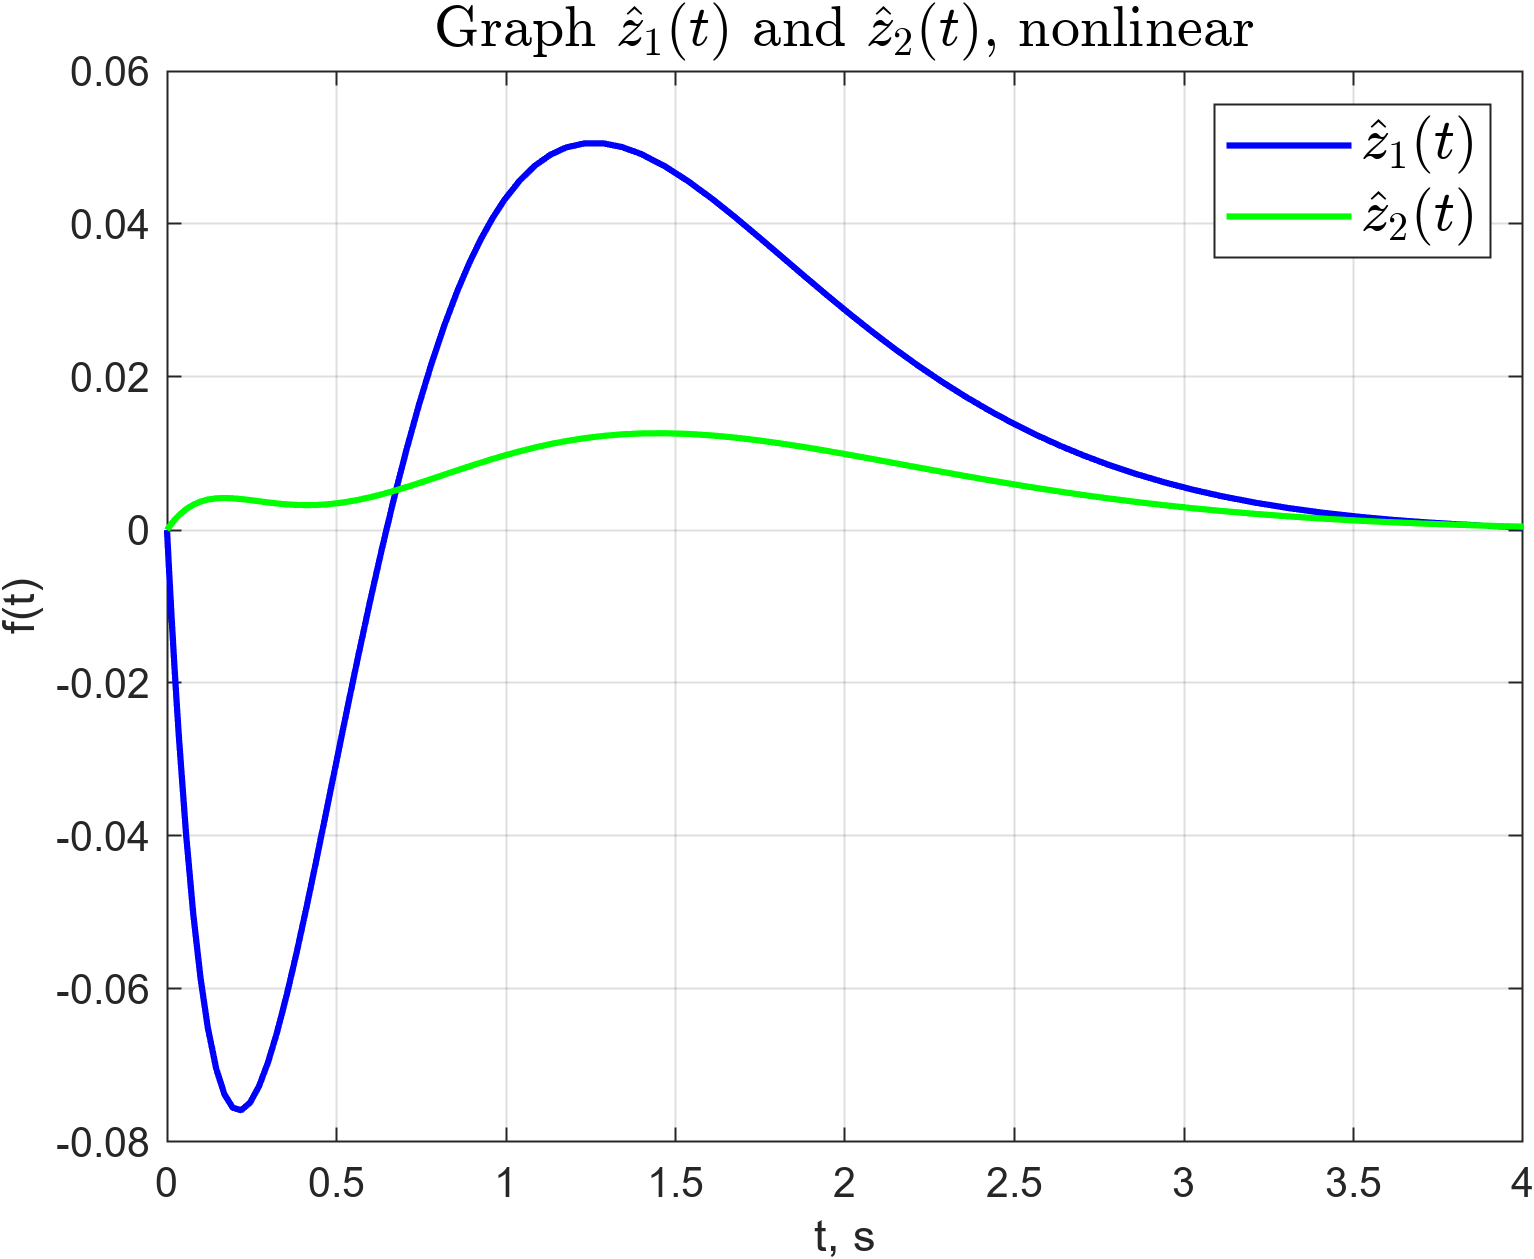
\includegraphics[width=0.6\linewidth]{pic/3_z_nlin_02_LW1.png}}
\caption{График $\hat{z}(t)$ для $ \sigma (\Gamma) = \{ -1, -2 \}$.}
\label{3_z_nlin_02_LW1}
\end{figure}

\begin{figure}[!h]
\center{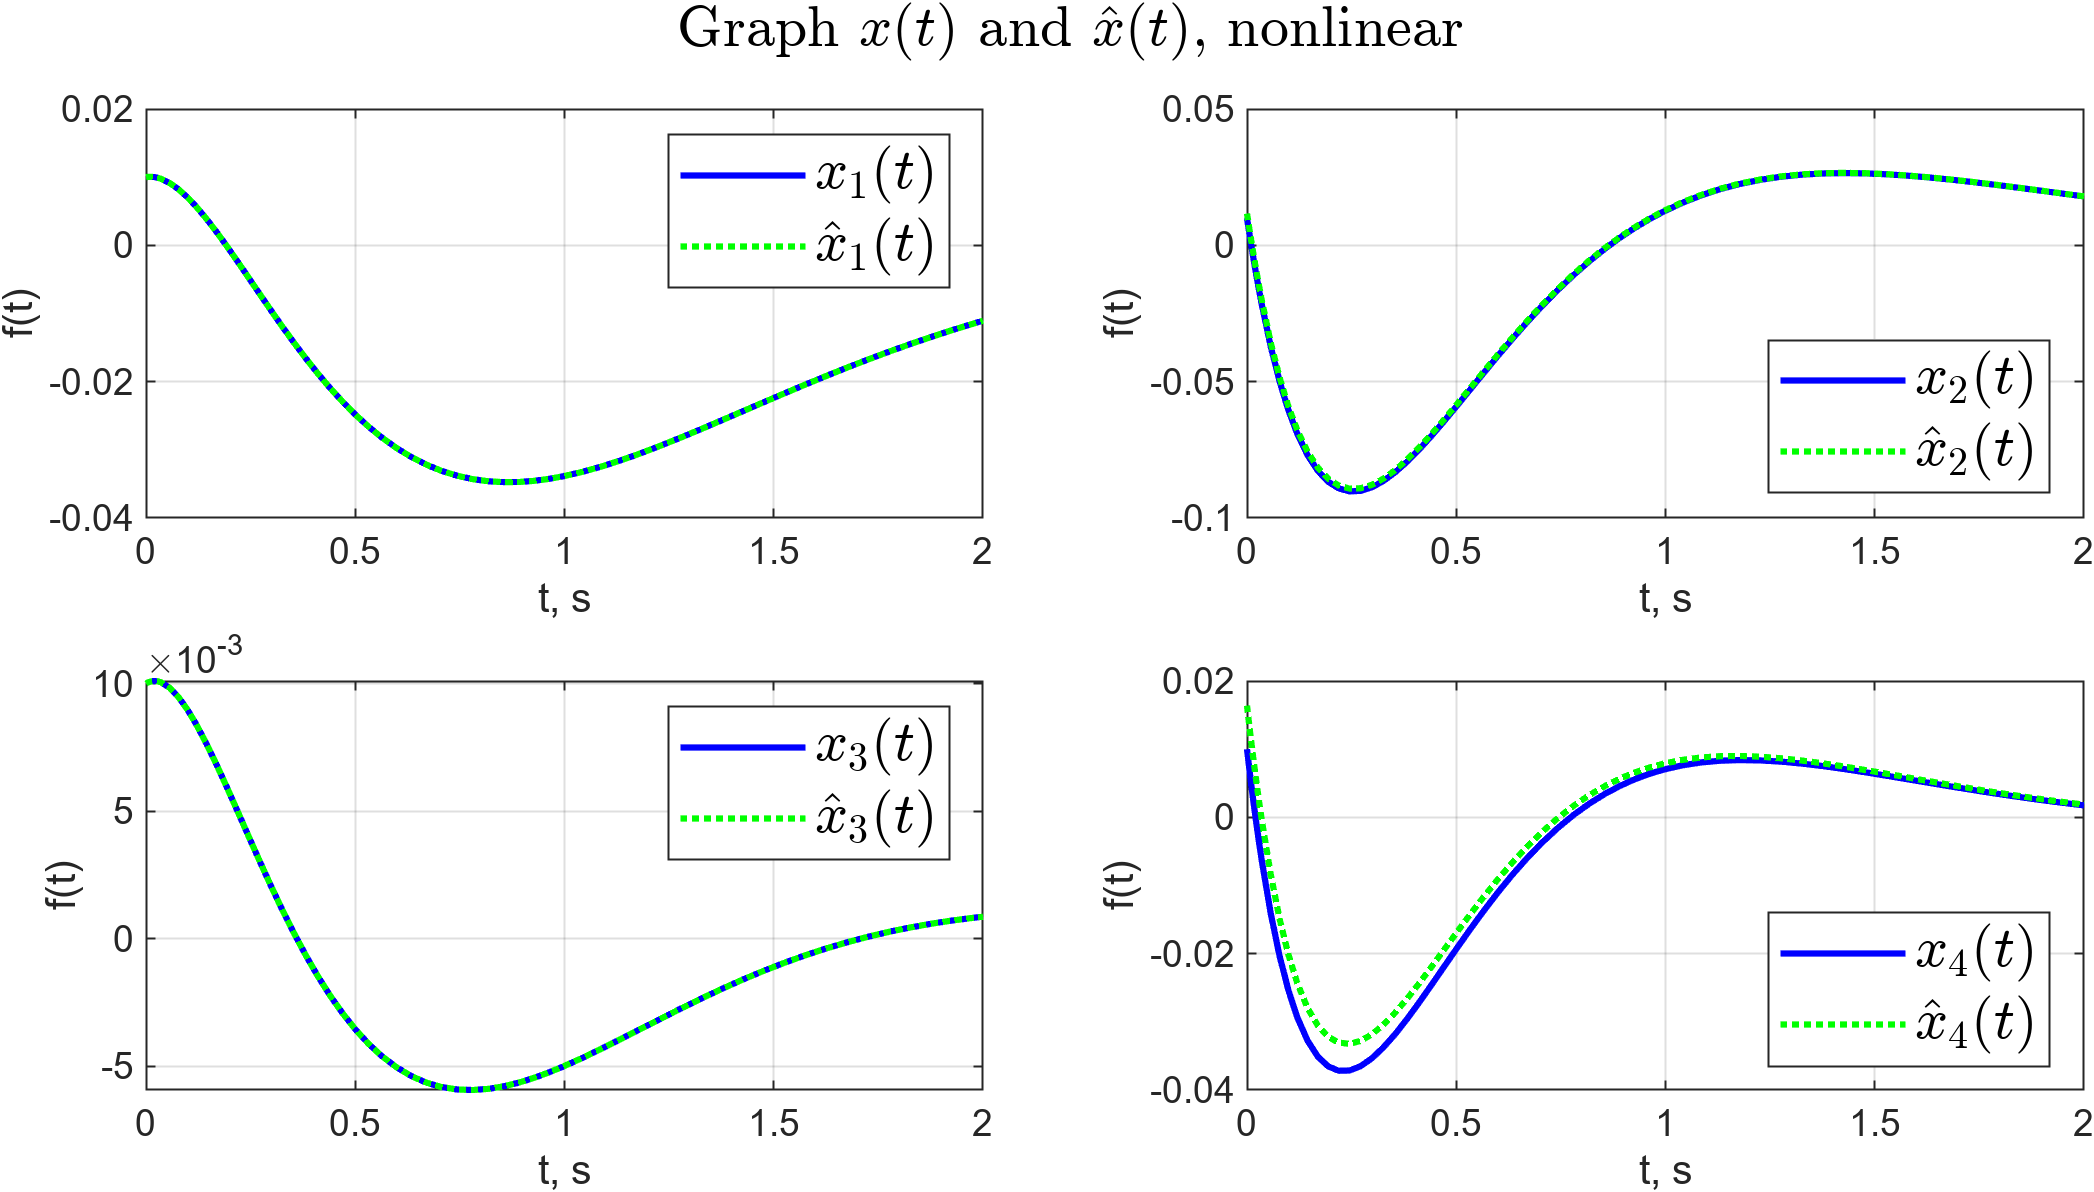
\includegraphics[width=1\linewidth]{pic/3_xx_nlin_02_LW1.png}}
\caption{Графики $x(t)$ и $\hat{x}(t)$ для $ \sigma (\Gamma) = \{ -1, -2 \}$.}
\label{3_xx_nlin_02_LW1}
\end{figure}


\begin{figure}[!h]
\center{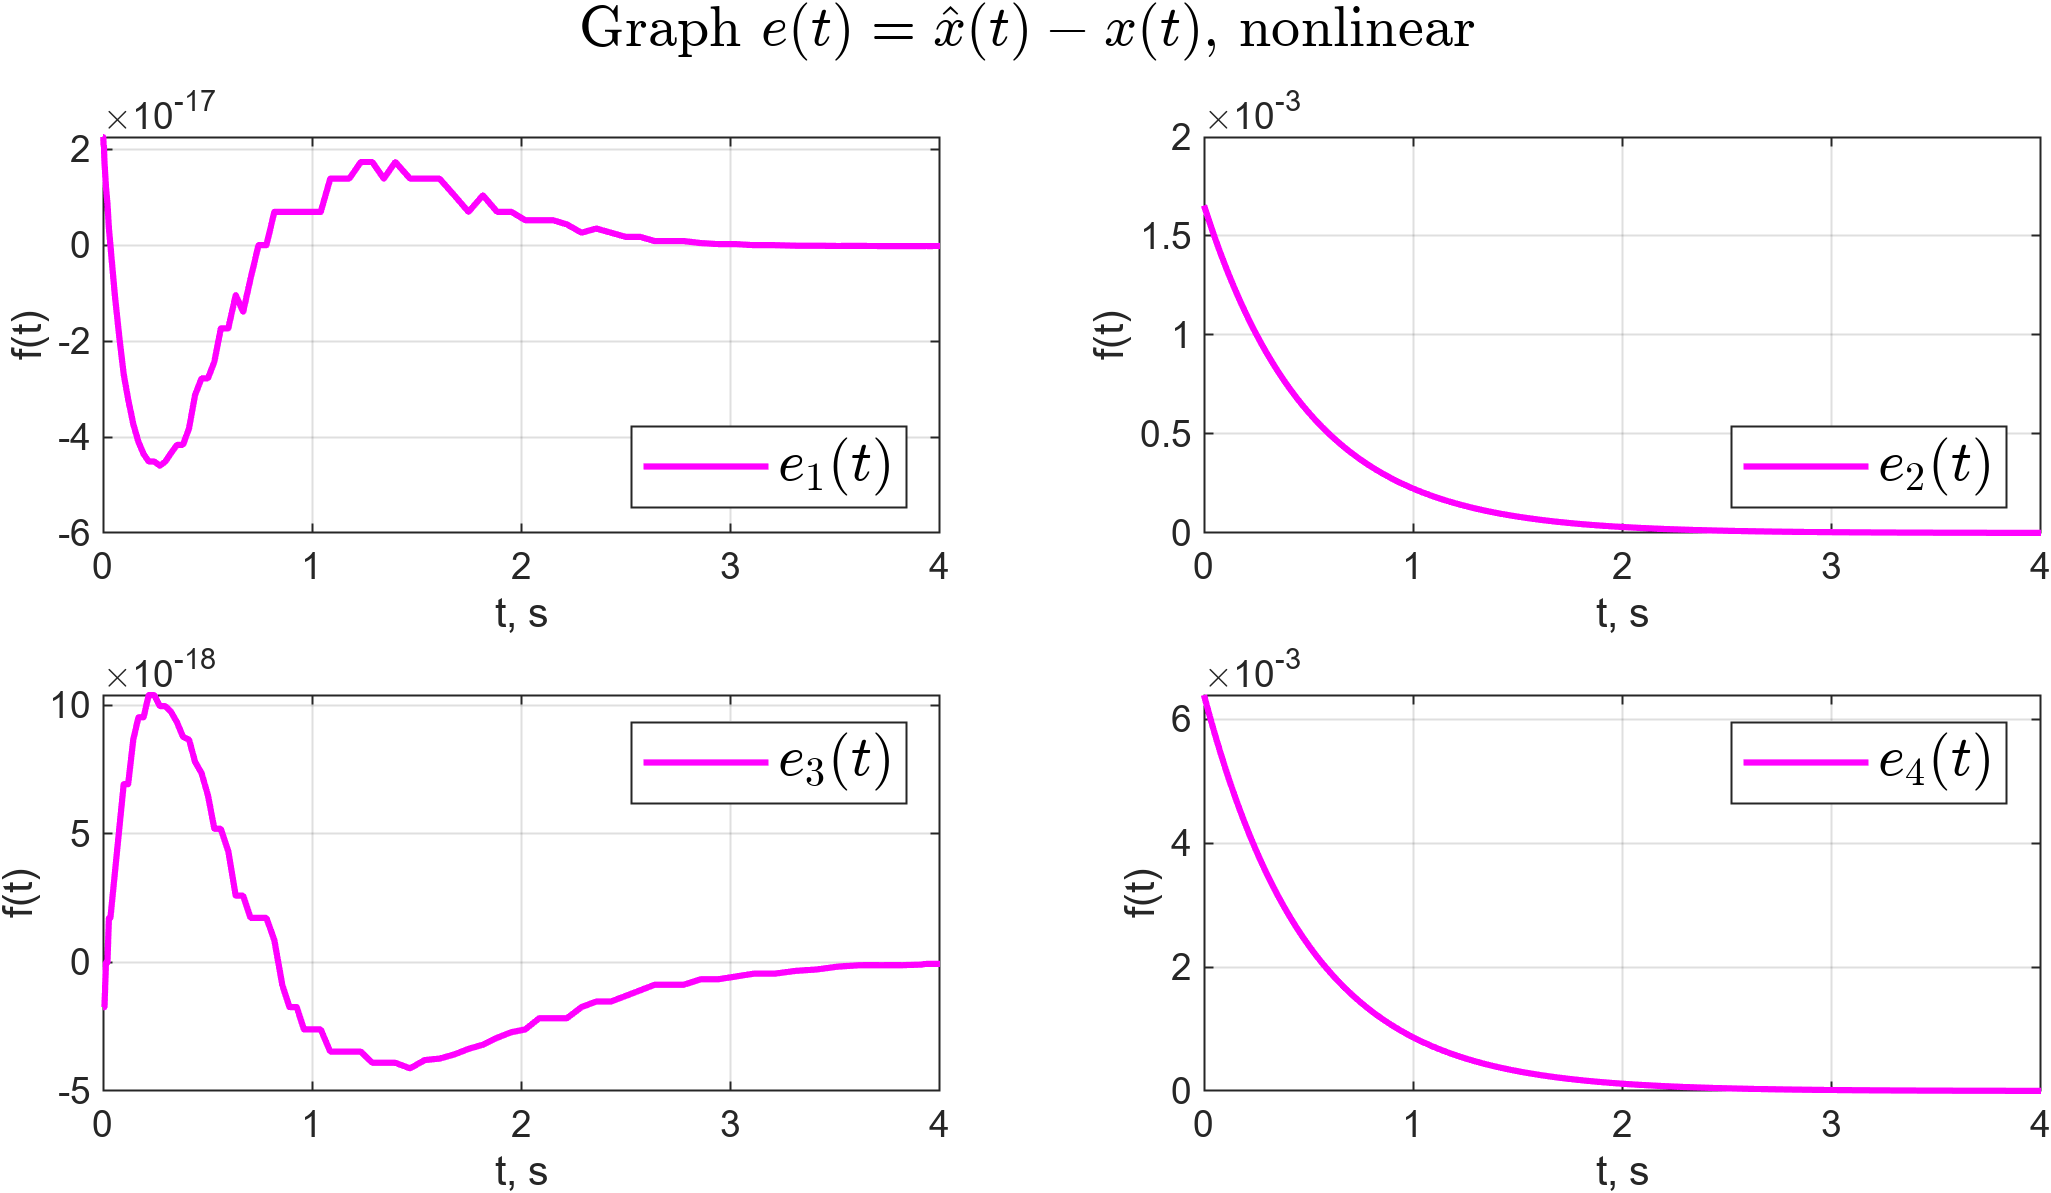
\includegraphics[width=1\linewidth]{pic/3_e_nlin_02_LW1.png}}
\caption{Графики $e (t) =\hat{x}(t) - x(t)$ для $ \sigma (\Gamma) = \{ -1, -2 \}$.}
\label{3_e_nlin_02_LW1}
\end{figure}

Рассмотрим работу наблюдателя пониженной размерности при значениях спектра 

\begin{equation*}
  \begin{matrix}
      \sigma_1 = \{ -0.1, -0.2 \}, & \sigma_2 = \{ -10, -20 \},\\
      \sigma_3 = \{ -2  \pm i \} & 
 \end{matrix}
\end{equation*}

\begin{figure}[!h]
\center{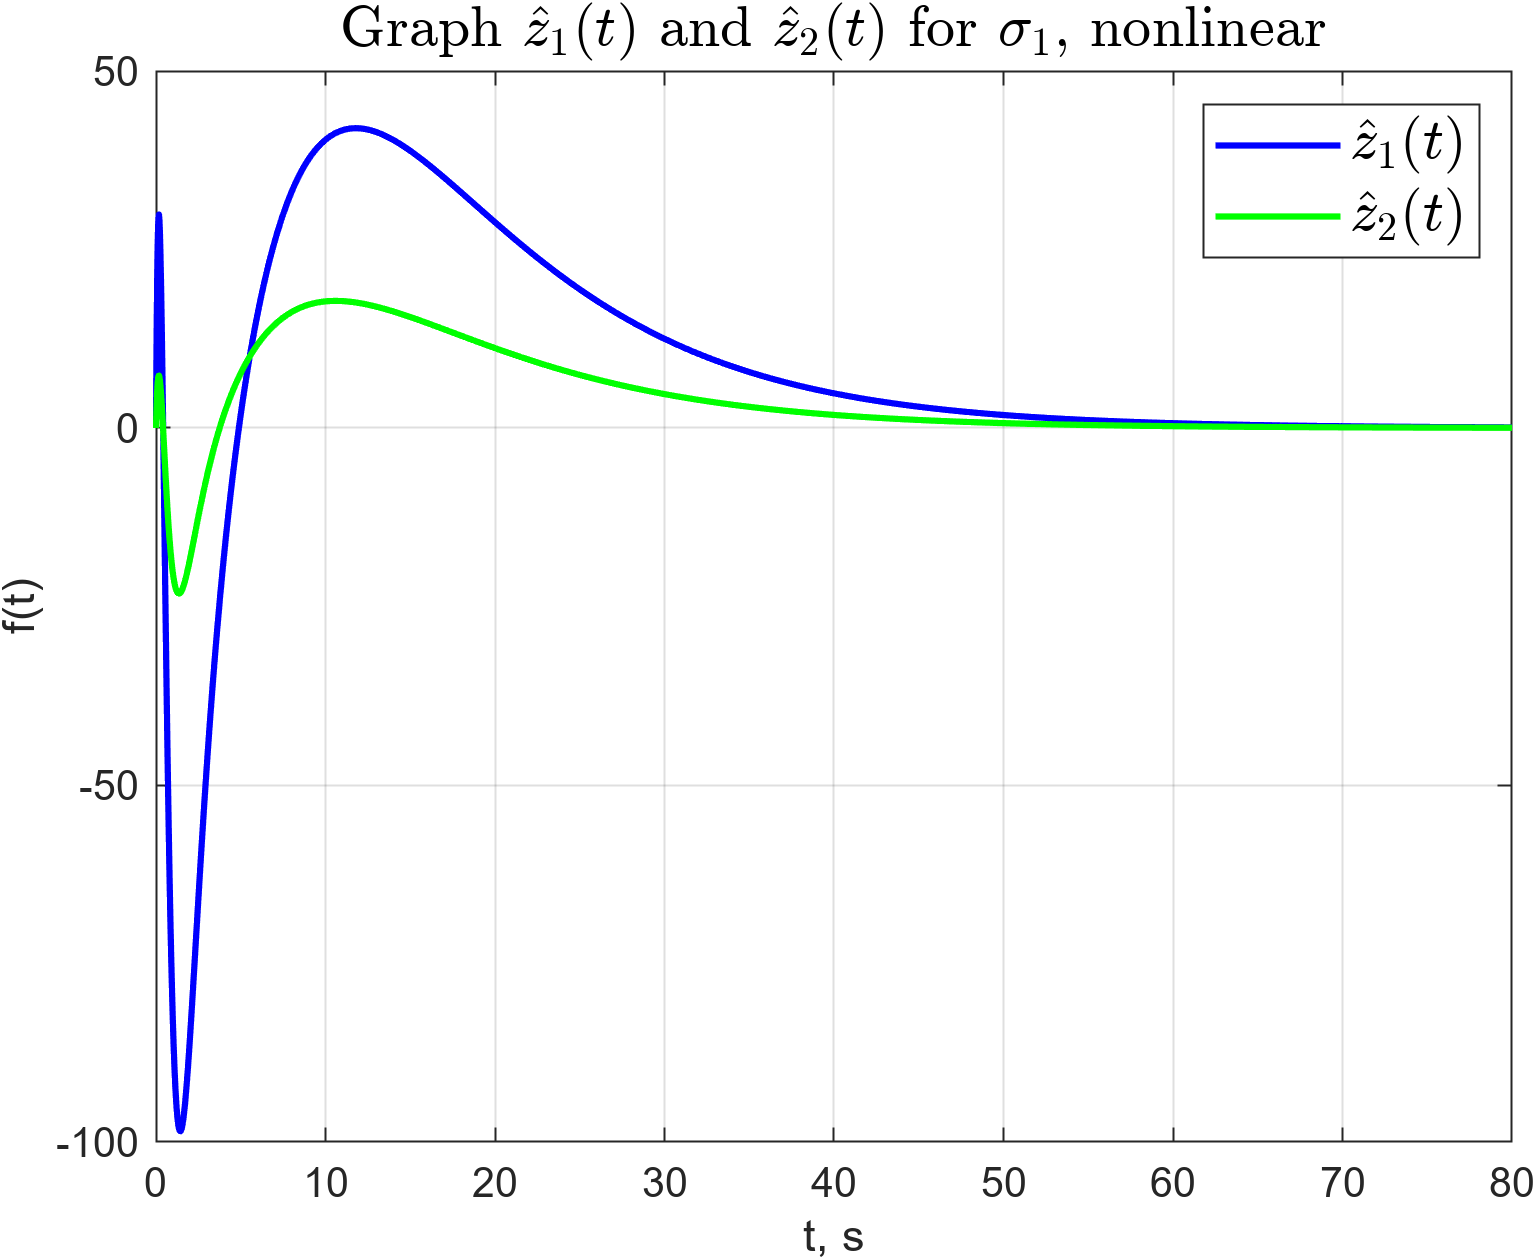
\includegraphics[width=0.6\linewidth]{pic/3_z_nlin_02_LW2.png}}
\caption{График $\hat{z}(t)$ для $ \sigma_1 (\Gamma) = \{ -0.1, -0.2 \}$.}
\label{3_z_nlin_02_LW2}
\end{figure}

\begin{figure}[!h]
\center{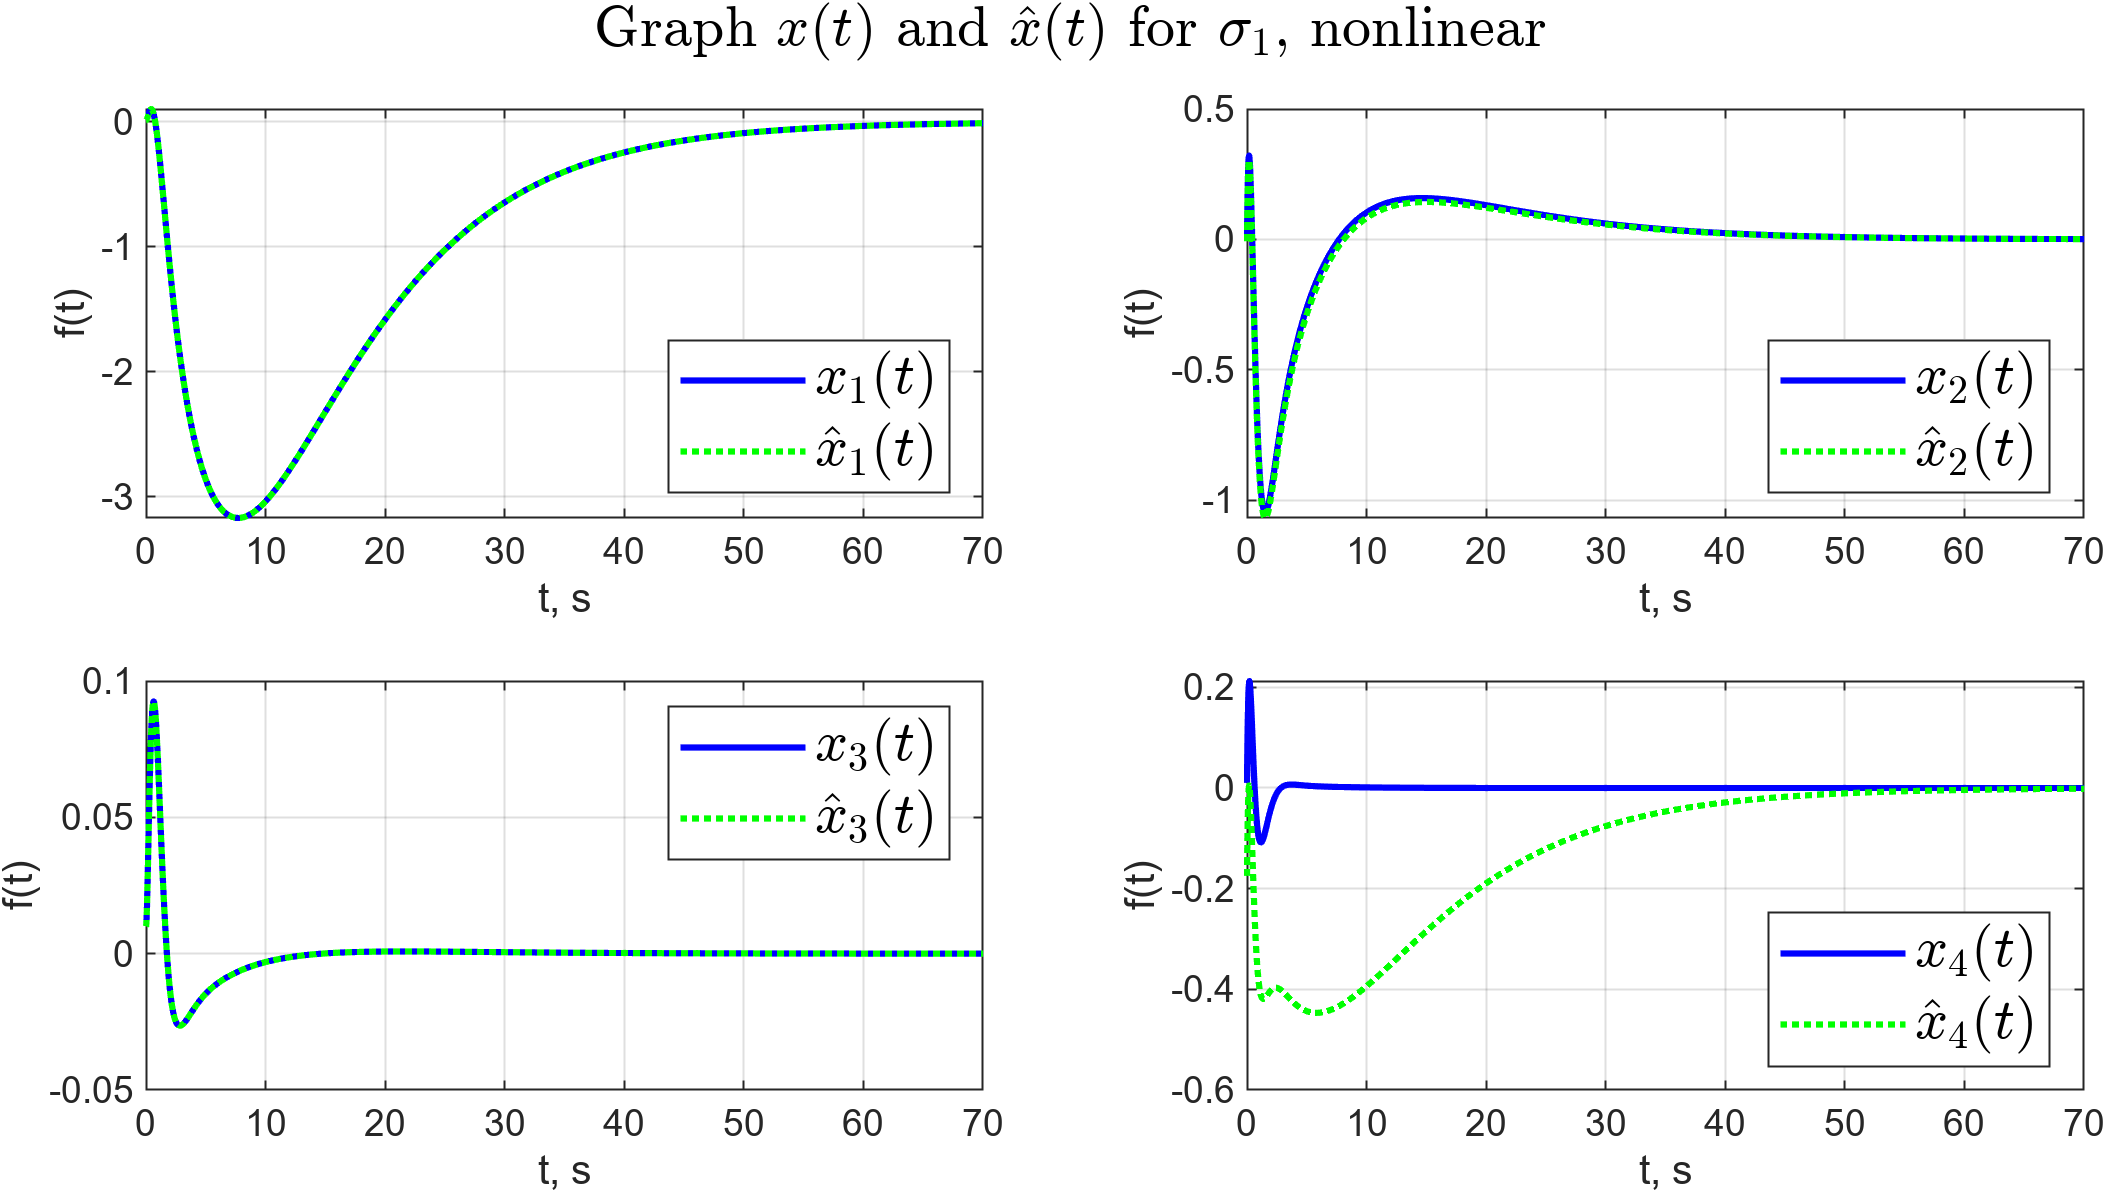
\includegraphics[width=1\linewidth]{pic/3_xx_nlin_02_LW2.png}}
\caption{Графики $x(t)$ и $\hat{x}(t)$ для $ \sigma_1 (\Gamma) = \{ -0.1, -0.2 \}$.}
\label{3_xx_nlin_02_LW2}
\end{figure}

\begin{figure}[!h]
\center{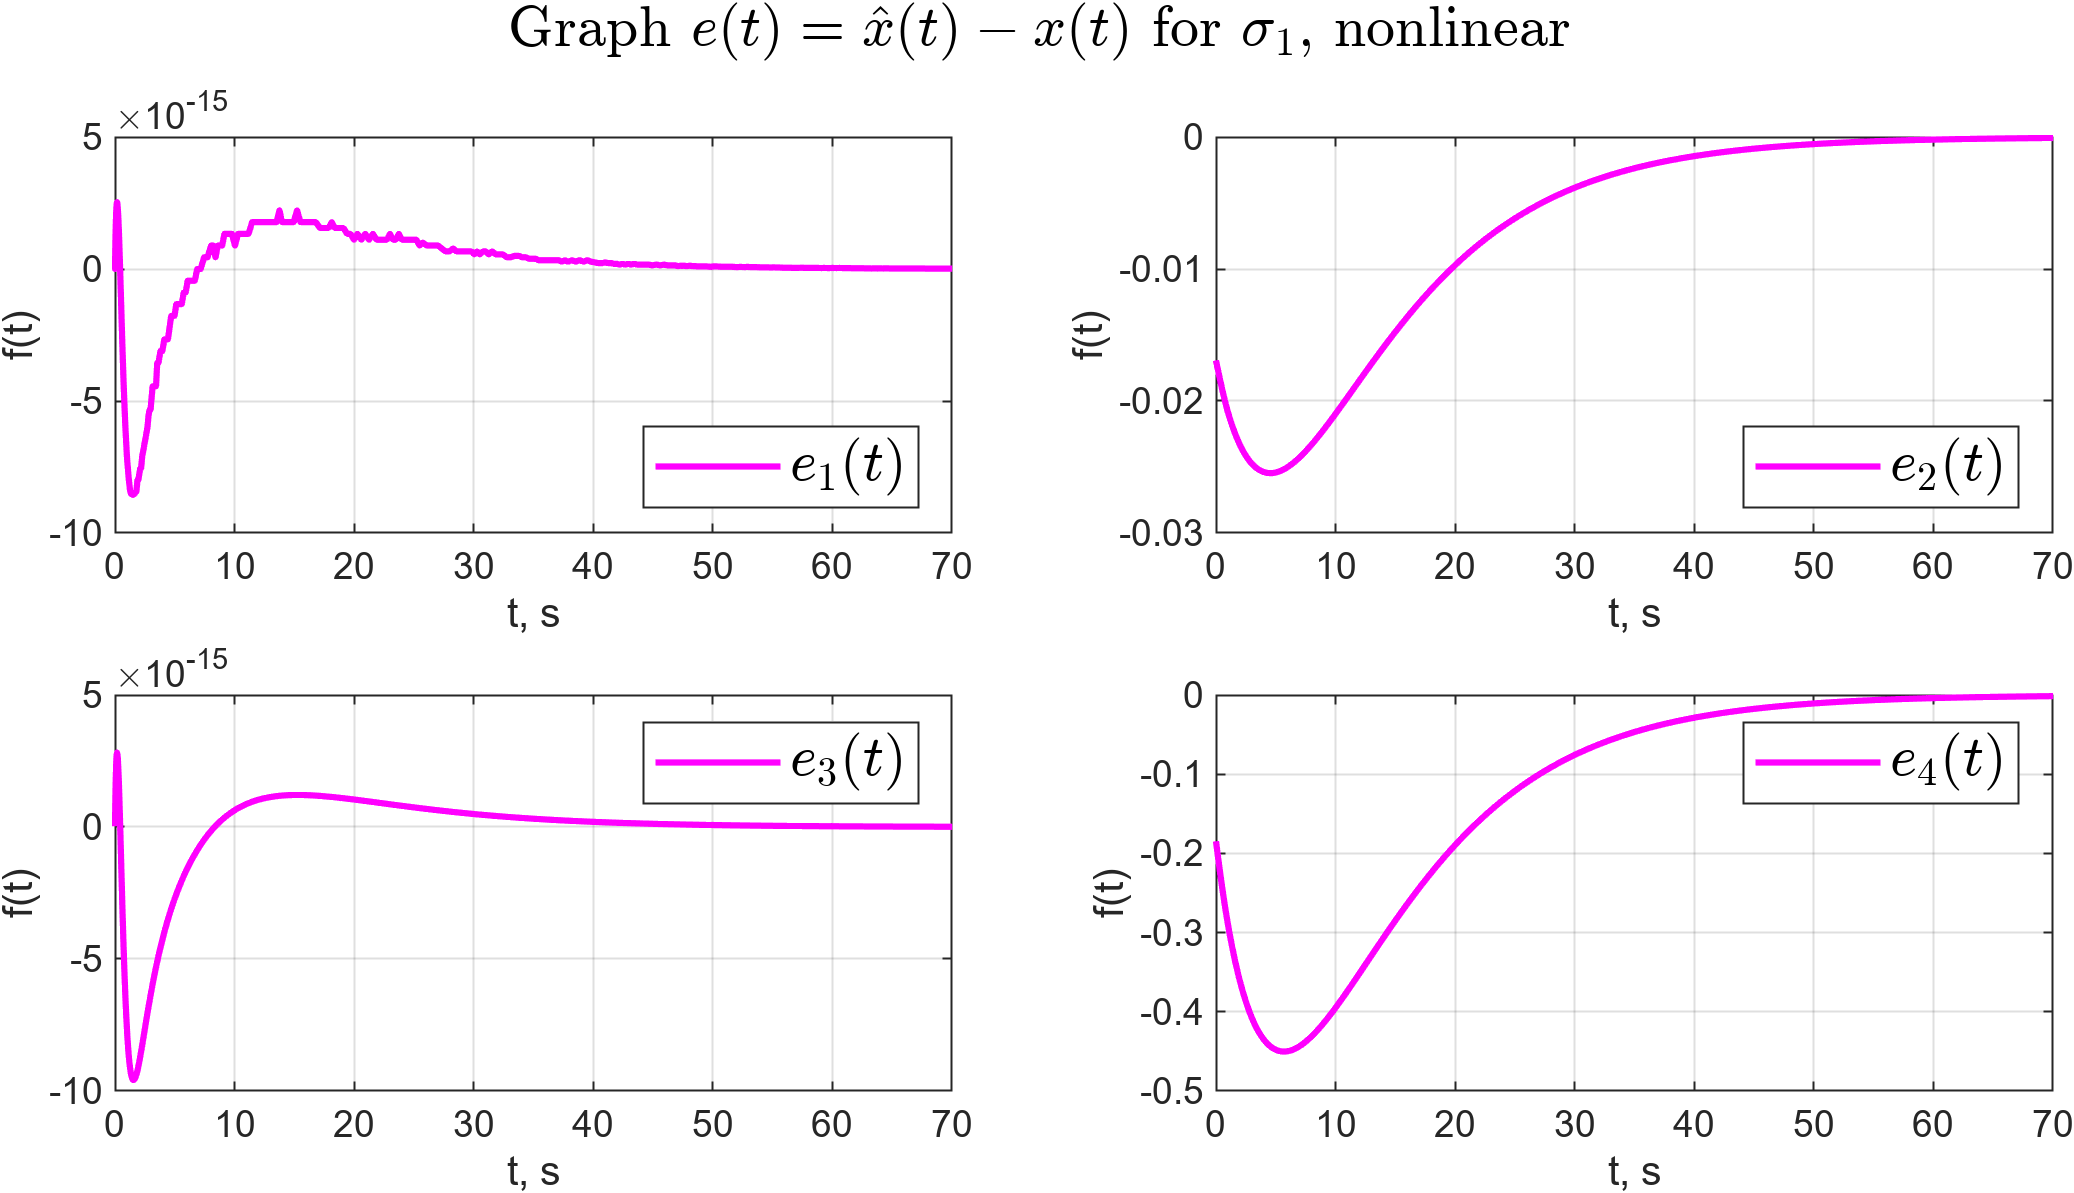
\includegraphics[width=1\linewidth]{pic/3_e_nlin_02_LW2.png}}
\caption{Графики $e (t) =\hat{x}(t) - x(t)$ для $ \sigma_1 (\Gamma) = \{ -0.1, -0.2 \}$.}
\label{3_e_nlin_02_LW2}
\end{figure}


\begin{figure}[!h]
\center{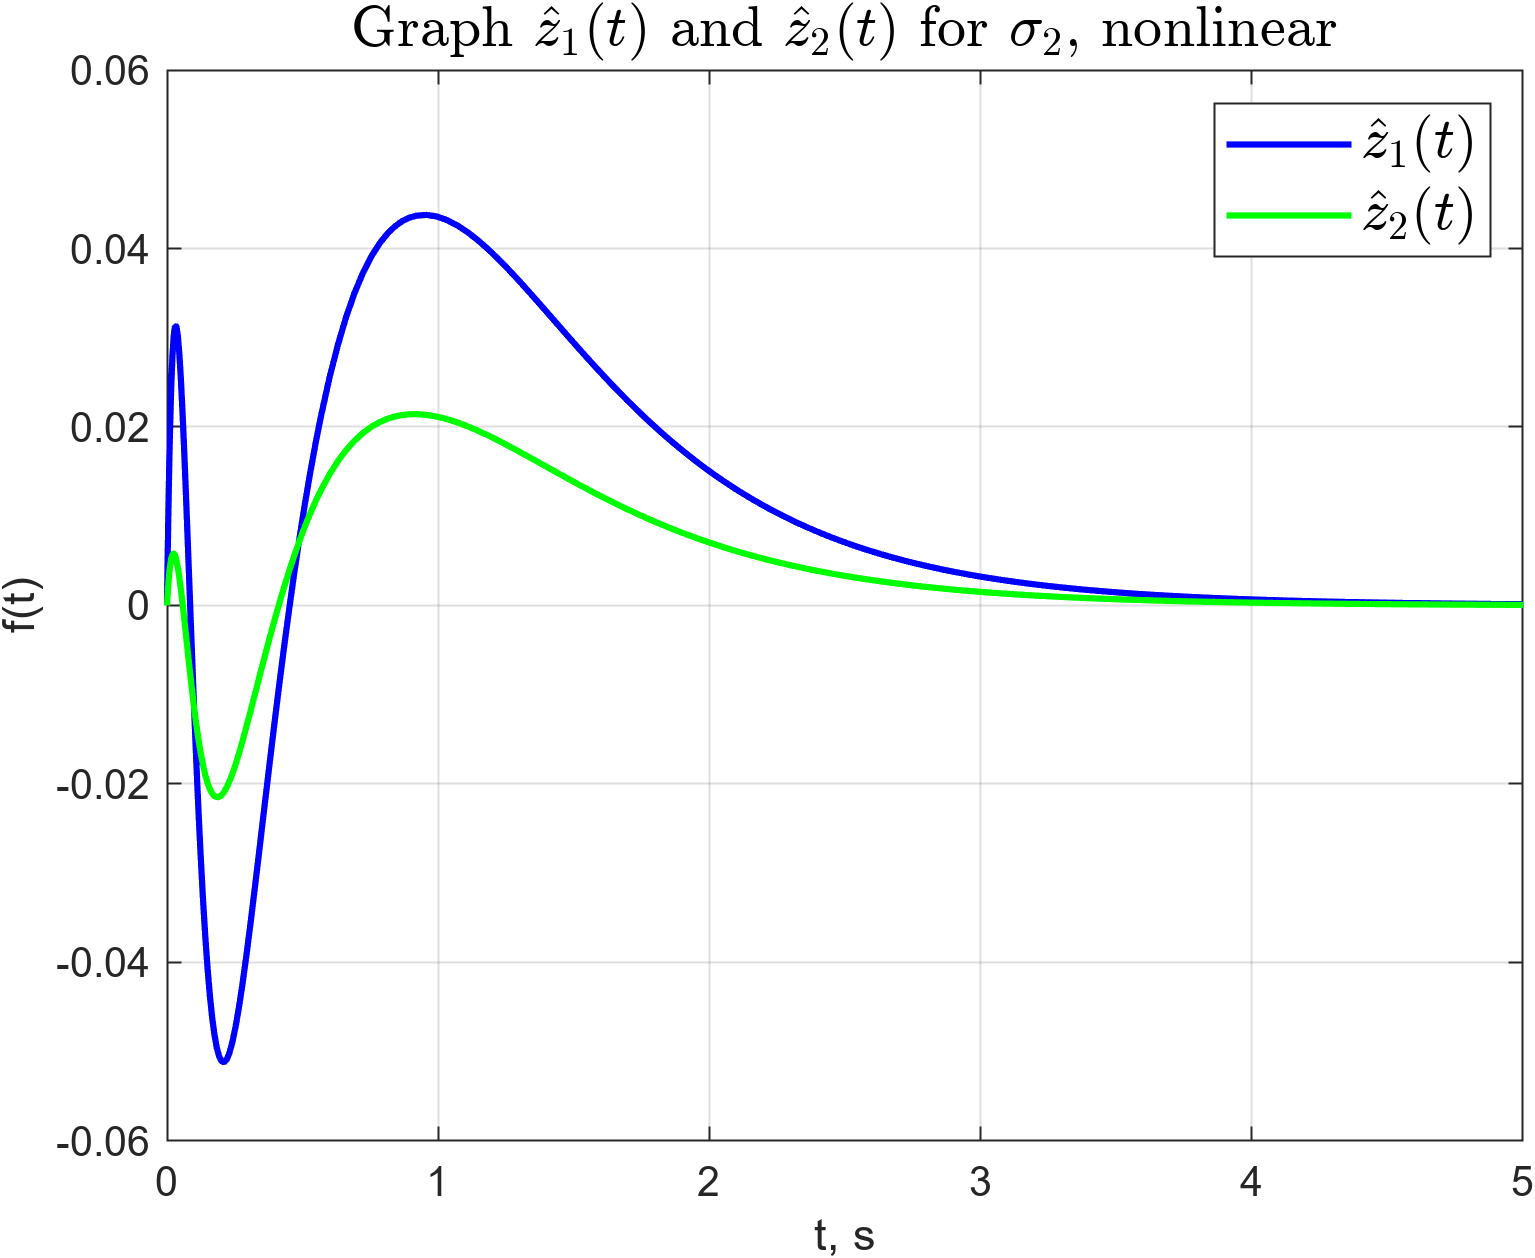
\includegraphics[width=0.6\linewidth]{pic/3_z_nlin_02_LW3.png}}
\caption{График $\hat{z}(t)$ для $ \sigma_2 (\Gamma) = \{ -10, -20 \}$.}
\label{3_z_nlin_02_LW3}
\end{figure}

\begin{figure}[!h]
\center{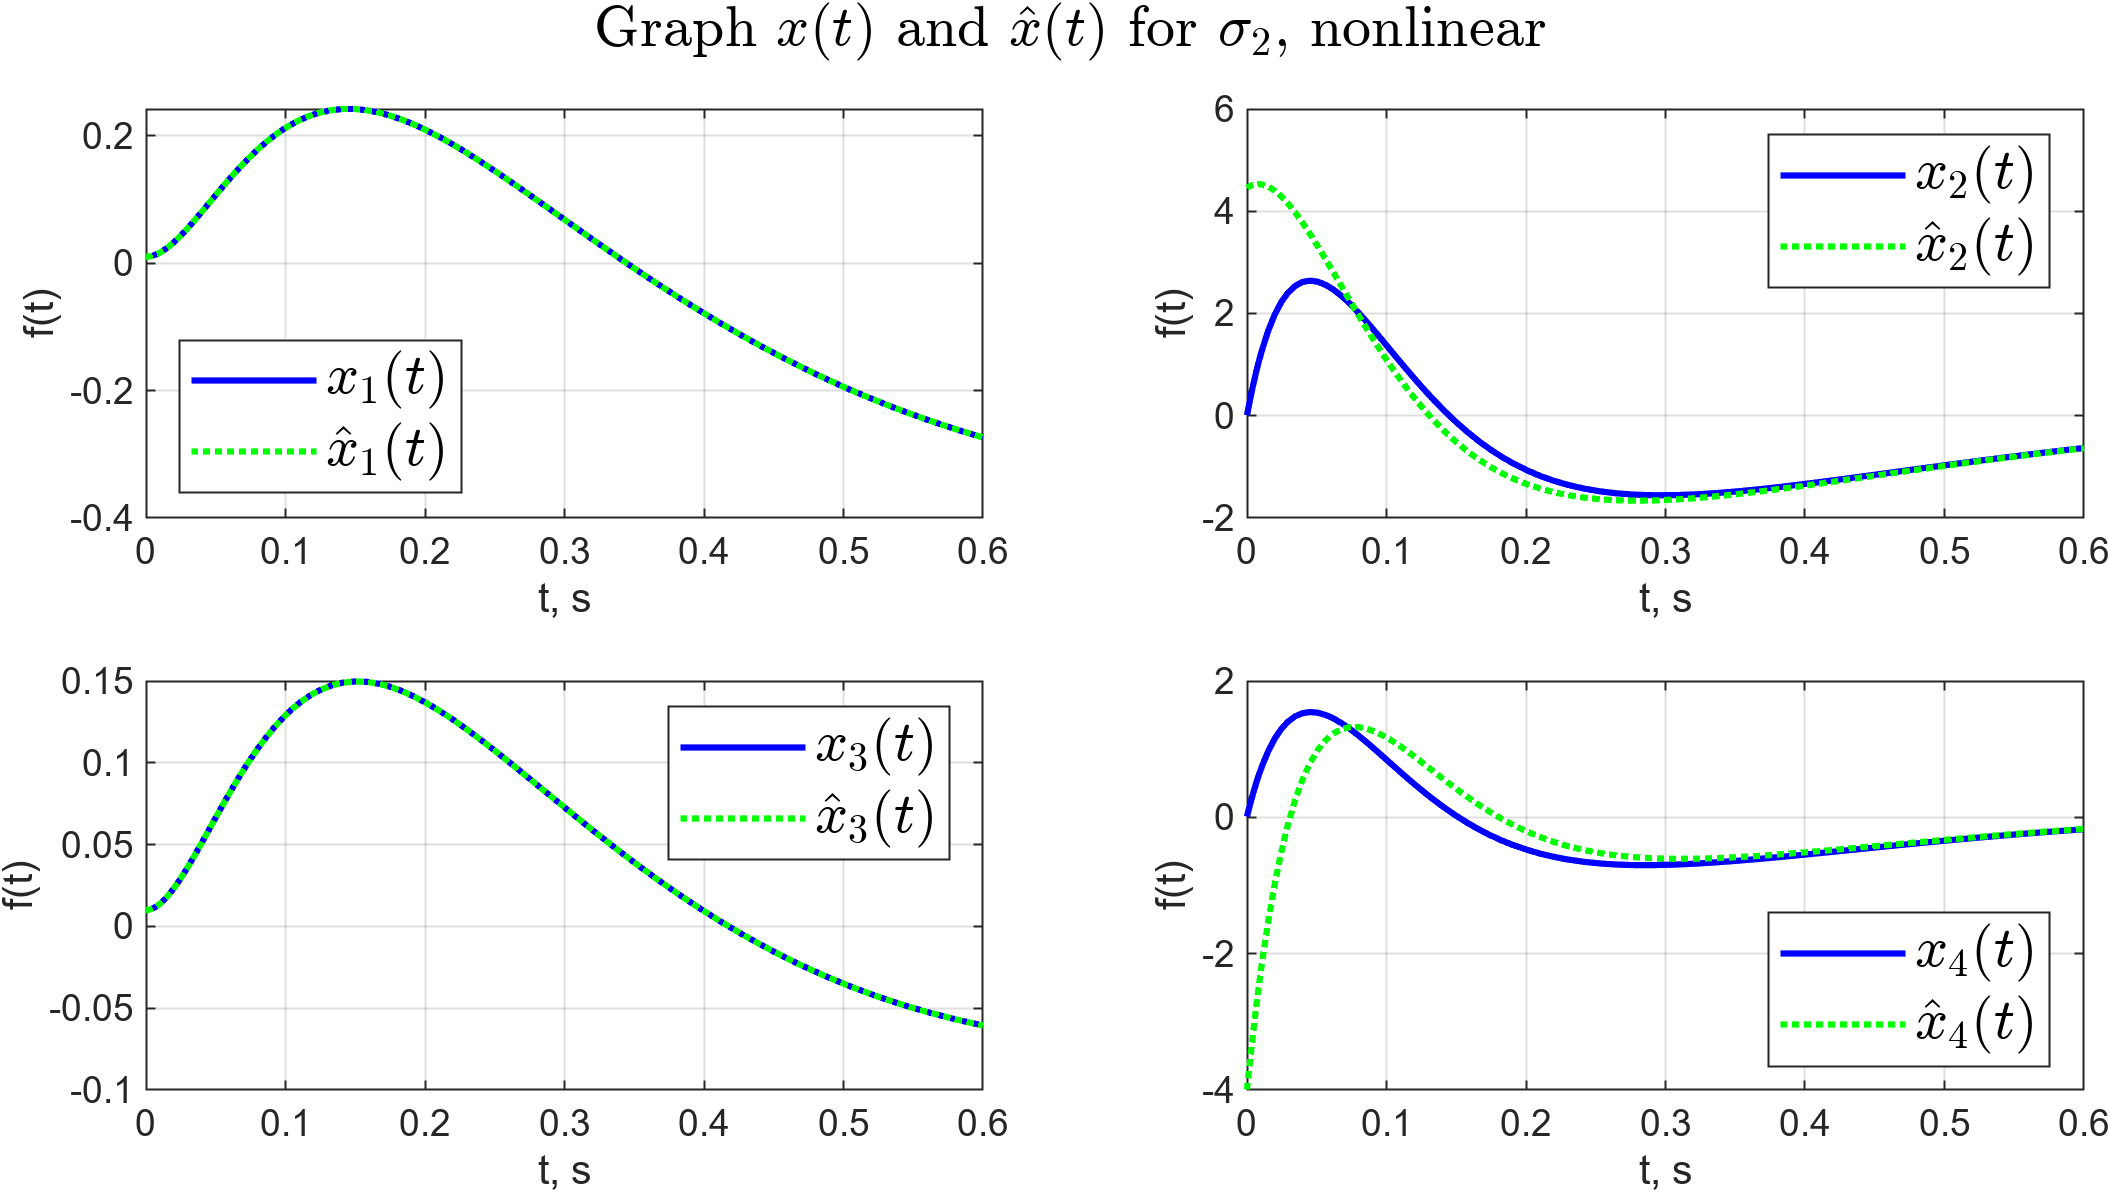
\includegraphics[width=1\linewidth]{pic/3_xx_nlin_02_LW3.png}}
\caption{Графики $x(t)$ и $\hat{x}(t)$ для $ \sigma_2 (\Gamma) = \{ -10, -20 \}$.}
\label{3_xx_nlin_02_LW3}
\end{figure}

\begin{figure}[!h]
\center{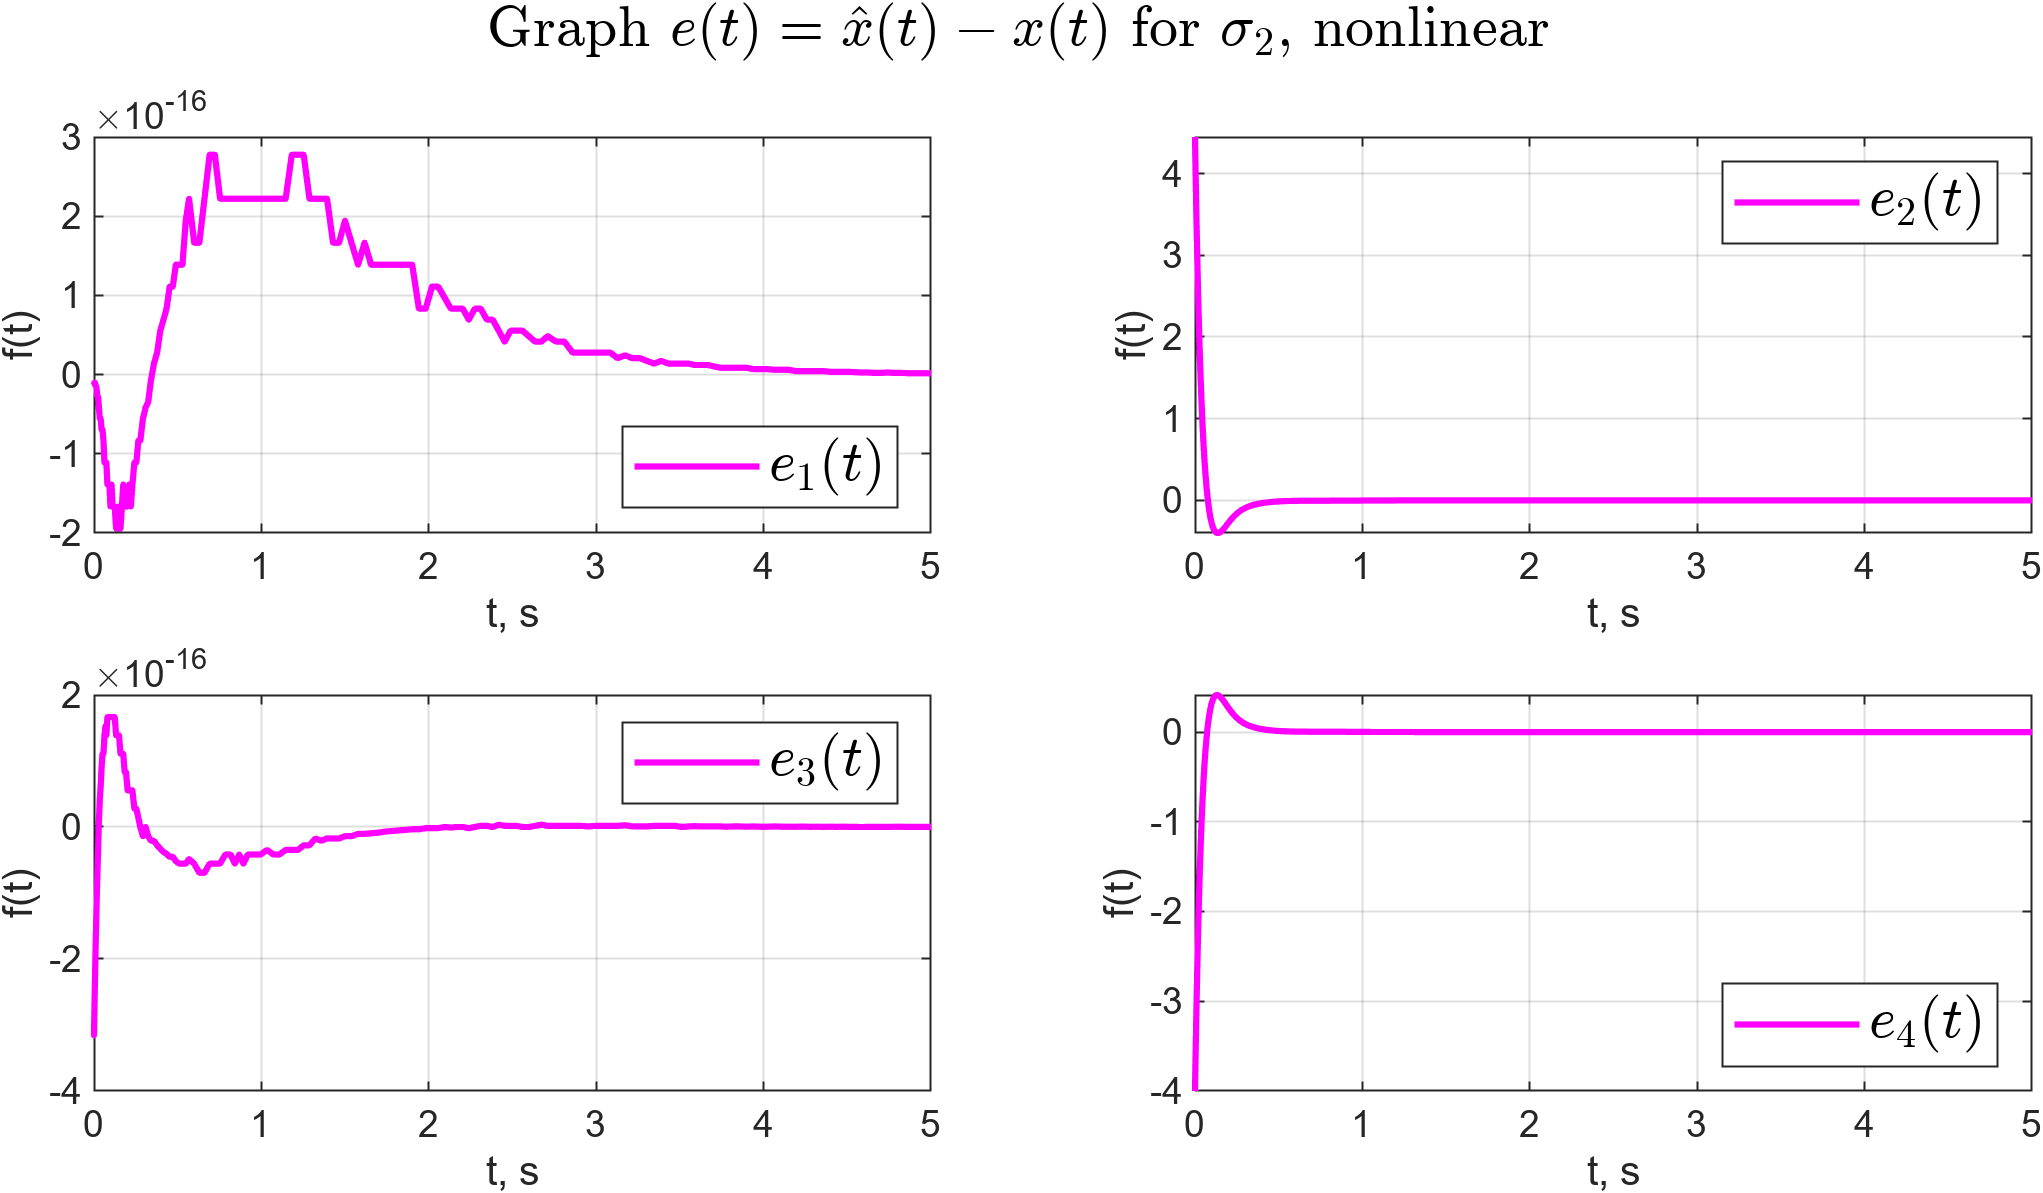
\includegraphics[width=1\linewidth]{pic/3_e_nlin_02_LW3.png}}
\caption{Графики $e (t) =\hat{x}(t) - x(t)$ для $ \sigma_2 (\Gamma) = \{ -10, -20 \}$.}
\label{3_e_nlin_02_LW3}
\end{figure}


\begin{figure}[!h]
\center{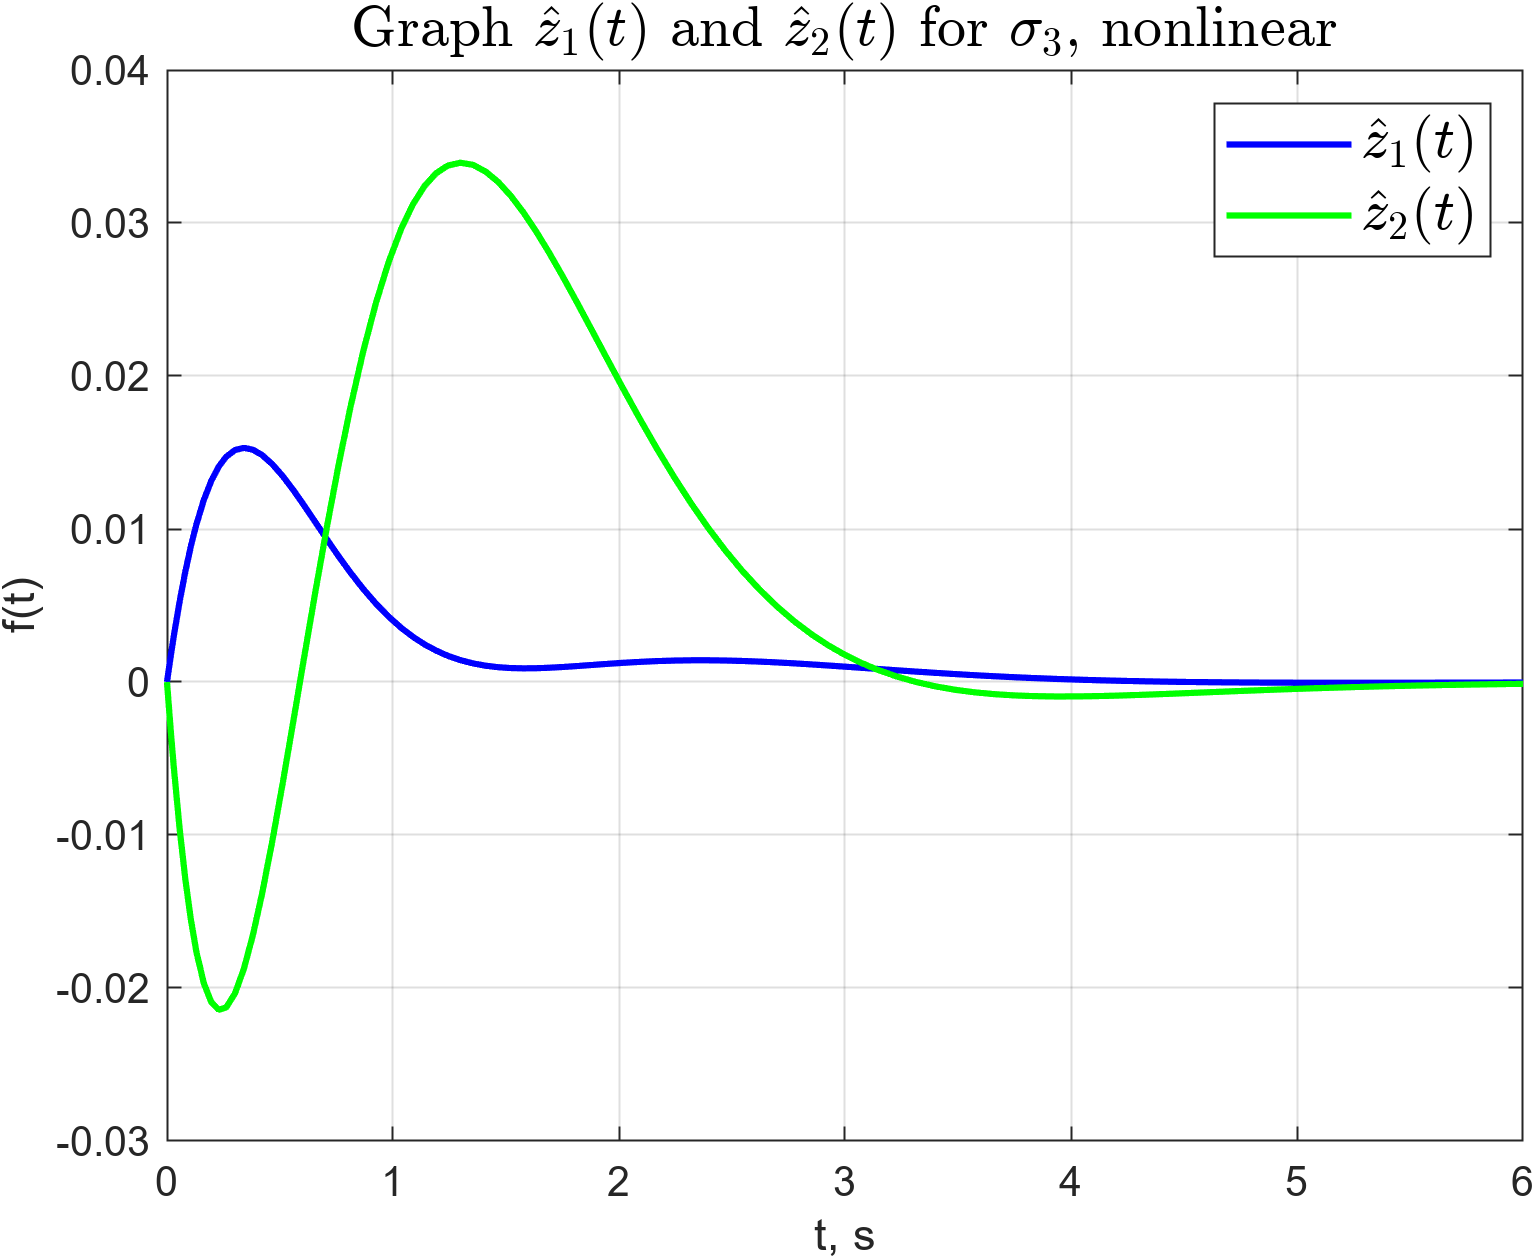
\includegraphics[width=0.6\linewidth]{pic/3_z_nlin_02_LW4.png}}
\caption{График $\hat{z}(t)$ для $ \sigma_3 (\Gamma) = \{ -2 \pm i \}$.}
\label{3_z_nlin_02_LW4}
\end{figure}

\begin{figure}[!h]
\center{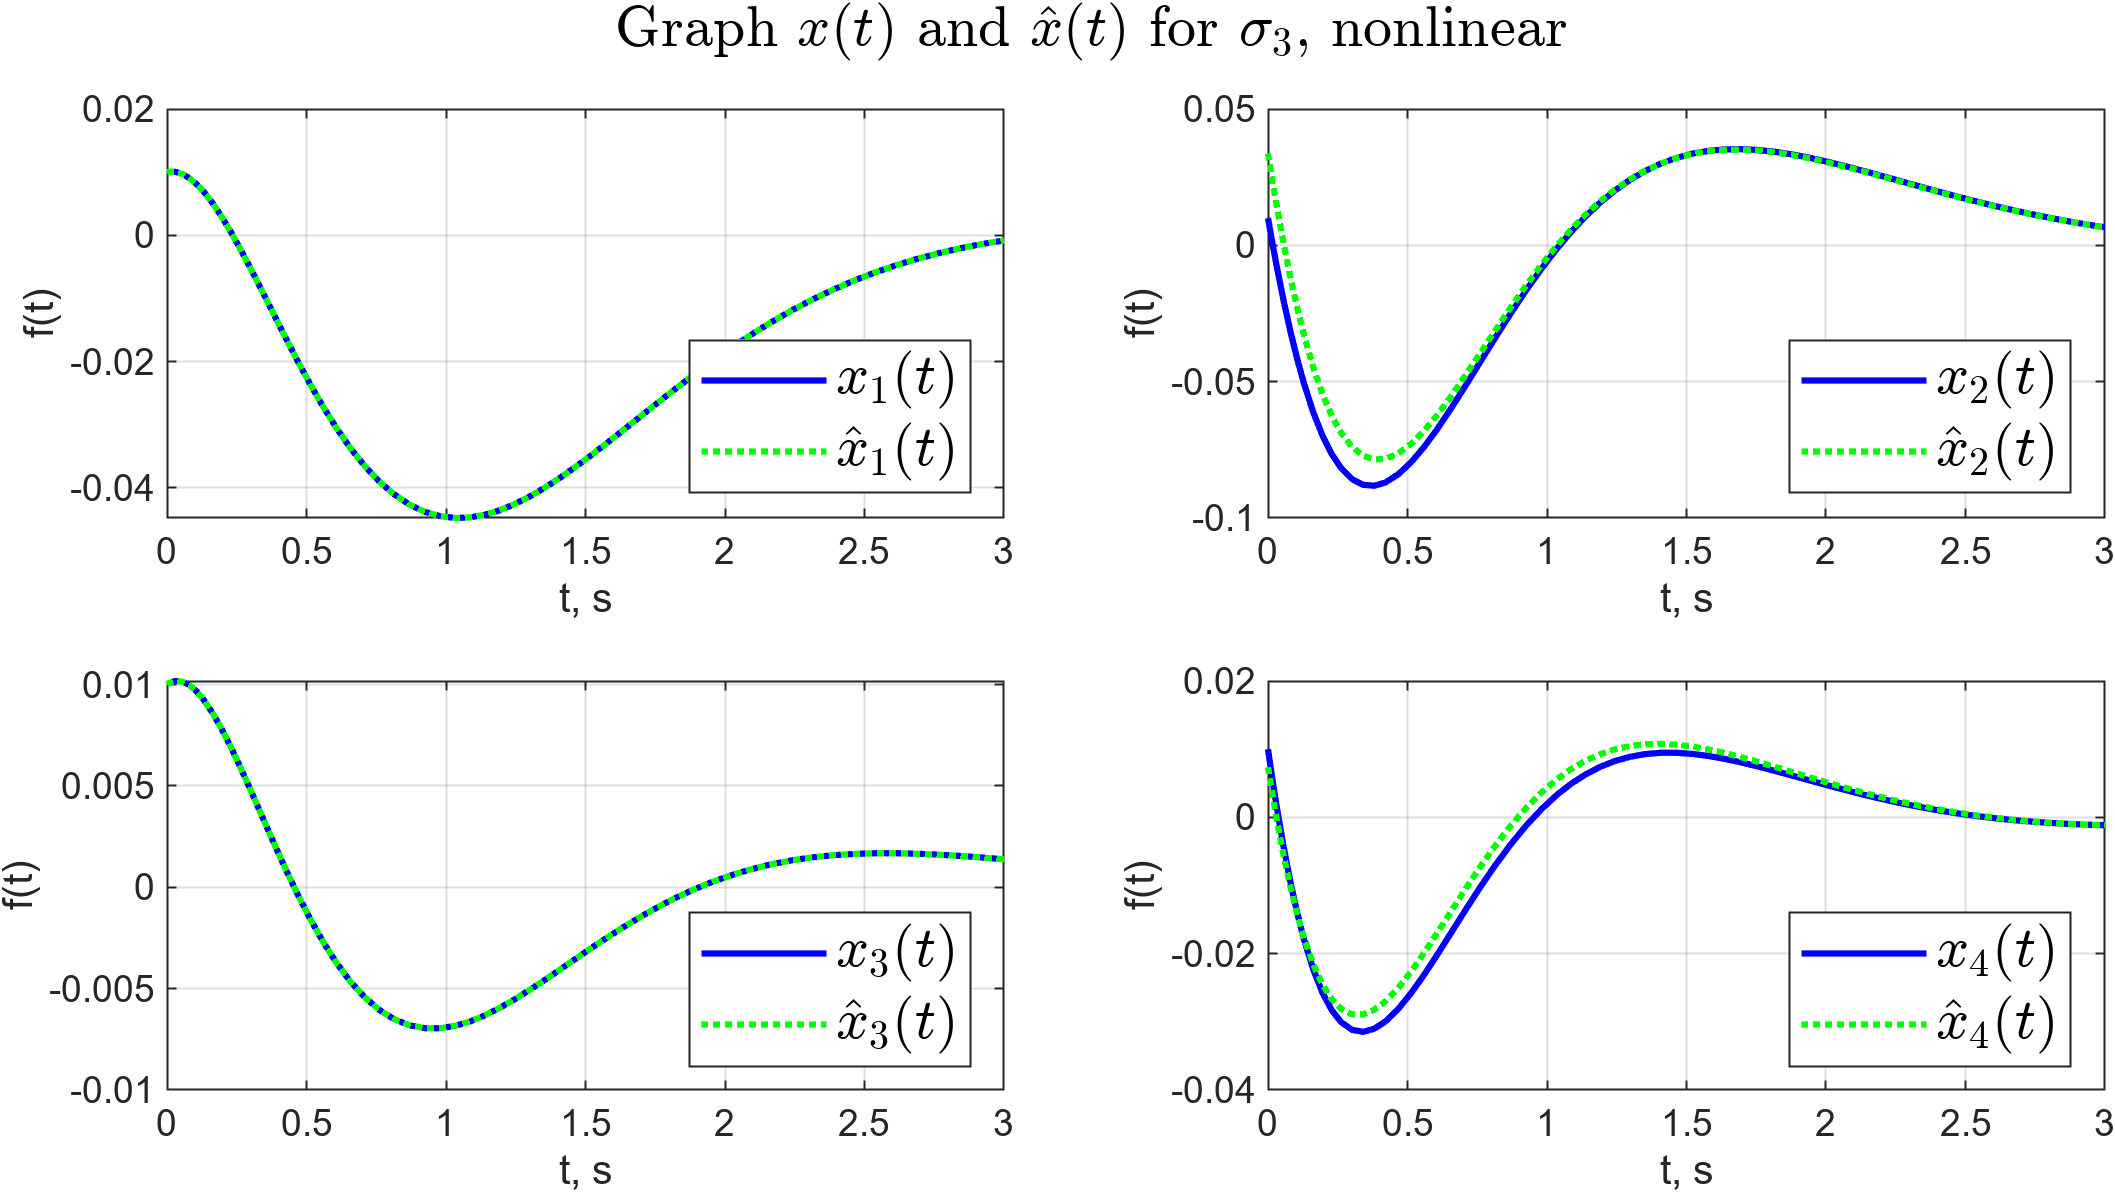
\includegraphics[width=1\linewidth]{pic/3_xx_nlin_02_LW4.png}}
\caption{Графики $x(t)$ и $\hat{x}(t)$ для $ \sigma_3 (\Gamma) = \{ -2 \pm i \}$.}
\label{3_xx_nlin_02_LW4}
\end{figure}

\begin{figure}[!h]
\center{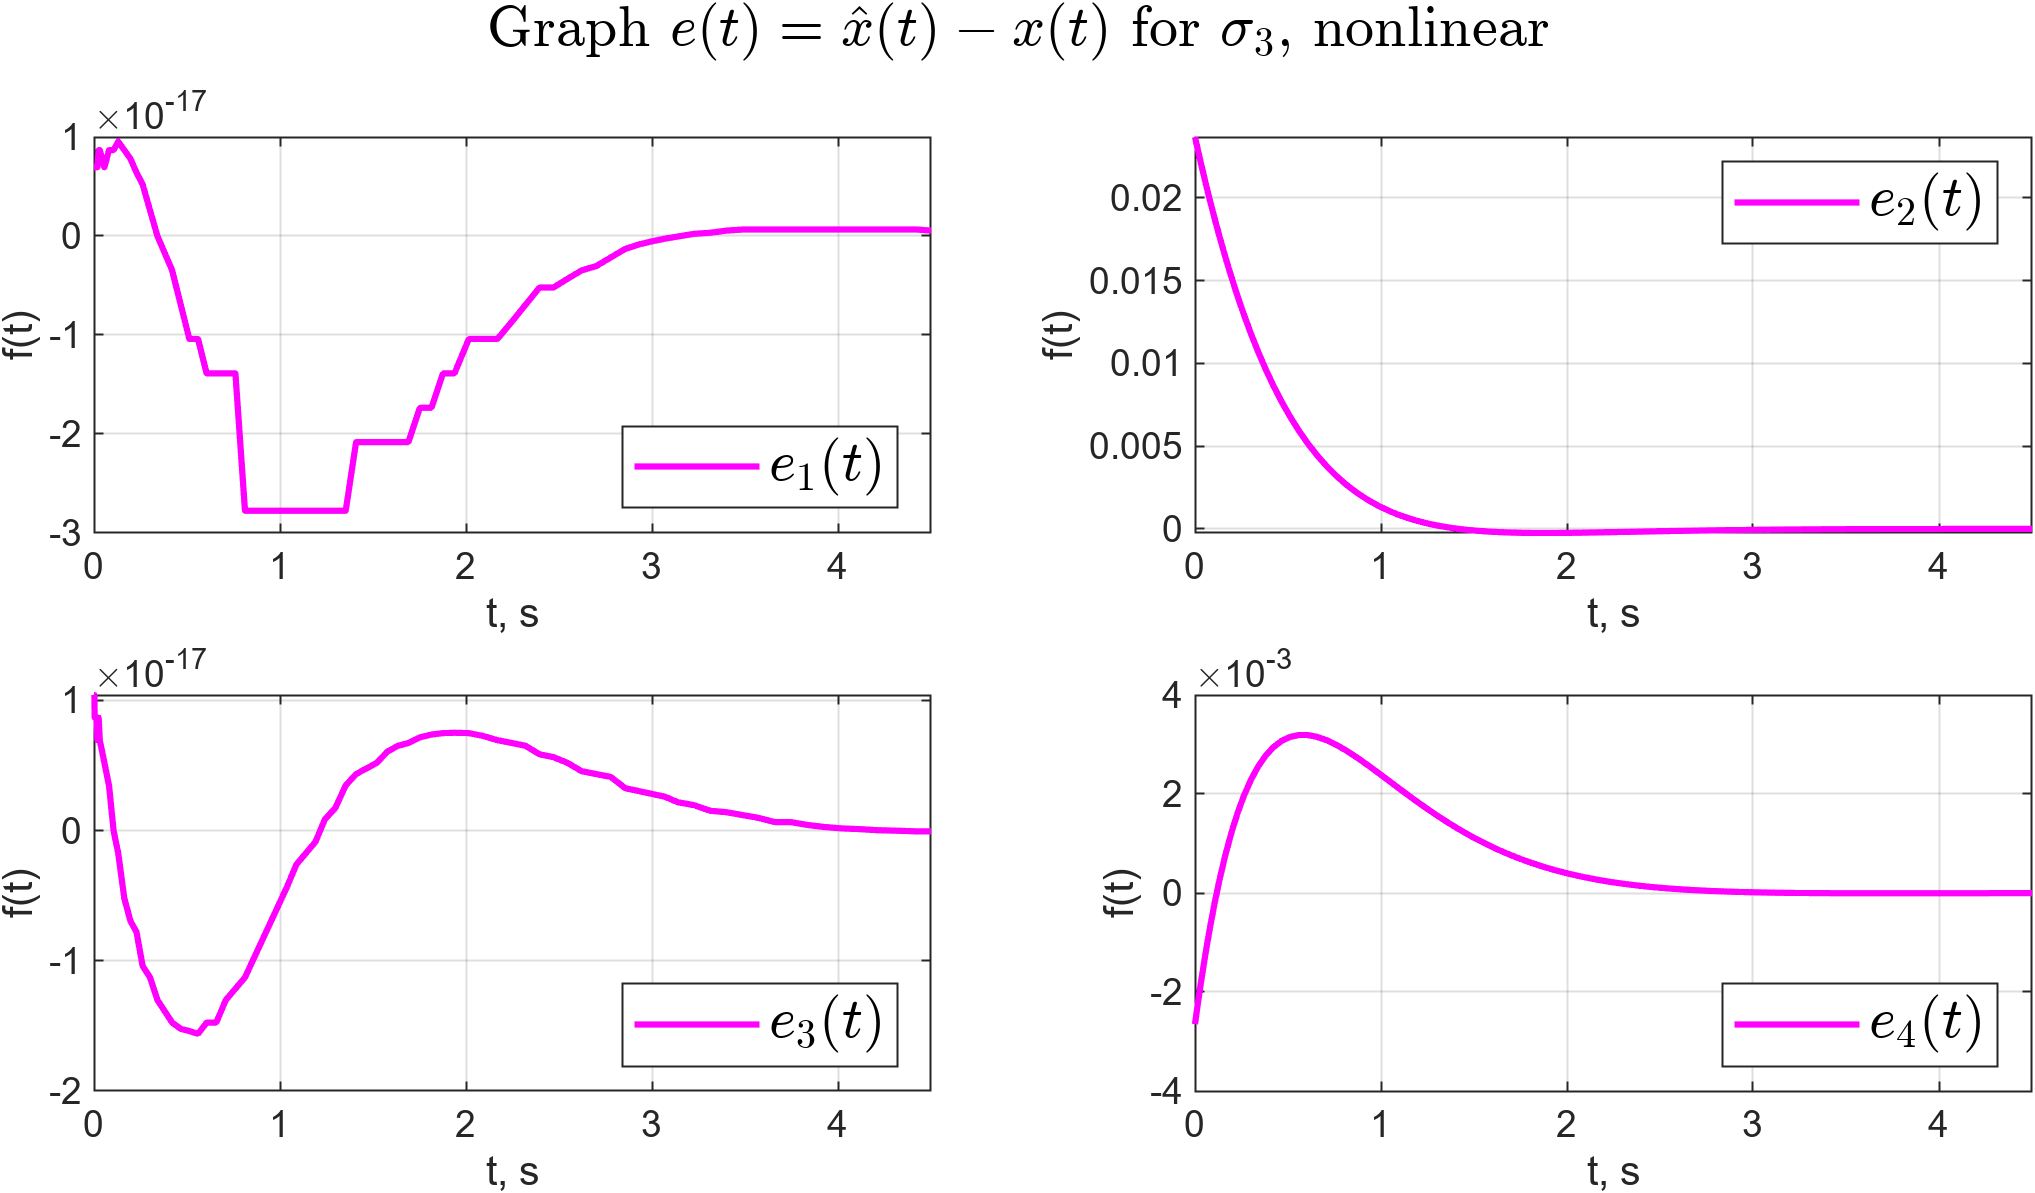
\includegraphics[width=1\linewidth]{pic/3_e_nlin_02_LW4.png}}
\caption{Графики $e (t) =\hat{x}(t) - x(t)$ для $ \sigma_3 (\Gamma) = \{ -2 \pm i \}$.}
\label{3_e_nlin_02_LW4}
\end{figure}





\newpage
\,
\newpage
\,
\newpage
\,
\newpage
Как и в случае наблюдателя полной размерности, для наблюдателя пониженной размерности также время, за которое ошибка наблюдателя становится неотличима от нуля, возрастает при уменьшении собственных значений для наблюдателя (рисунок \ref{3_e_nlin_02_LW2}) и уменьшается, при увеличении собственных чисел (рисунок \ref{3_e_nlin_02_LW3}).

\subsection{Сравнение работы наблюдателей полной и пониженной размерности}

В ходе исследования для наблюдателя пониженной размерности были подобраны спектры близкие к соответствующим наборам собственных чисел для наблюдателя полной размерности. 

Время, за которое ошибка наблюдателя становится неотличима от нуля, сопоставимо для наблюдателей полной и пониженной размерности для близких спектров. 

Для наблюдателя пониженной размерности практически нулевая ошибка для $x_1$ и $x_3$, так как эти компоненты напрямую попадают в вывод $y_1$ и $y_2$ соответственно, то есть они измеримы. Наблюдатель полного порядка в данном случае избыточен и накапливает большую ошибку. 


\section{Синтез регулятора по выходу}
Построим регулятор, стабилизирующий маятник и тележку в условиях, когда измерению доступны только сигналы $y_1$ и $y_2$. Для этого будем использовать наблюдатель пониженной размерности из предыдущего пункта и основанный на нем закон управления

\begin{equation}
    u = K \hat{x}
\end{equation}

Постараемся подобрать такие спектры наблюдателя и регулятора, при которых переходные процессы в замкнутой системе будут иметь малое время переходного процесса, малое перерегулирование и малую величину управляющего воздействия. Поэтому для каждого набора спектров наблюдателя и регулятора будем находить  максимальные значения модуля координаты тележки $x_1(t)$, угла отклонения маятника от вертикали $x_3(t)$ и управляющего воздействия $u(t)$, а также фиксировать время переходного процесса (как последний момент времени, когда координата тележки или угол отклонения маятника отличался от нуля более, чем на 0.0001).

\begin{table}[h]
\centering
\caption{Результаты моделирования для различных наборов спектров}
\label{3_tab_2}
\begin{tabular}{ccccccc}
\toprule
$\sigma_{reg}$  & $\sigma_{obs}$  & $\max |\varphi|$ & $\max |a|$ & $\max |u|$& t, s \\
\midrule
$\{ -1, -1, -1, -1\}$  & $\{-1, -1.5 \}$  & 0.011  &  0.15  &  67 & 15  \\
$\{ -3, -2.5, -2, -1.5\}$  & $\{-1, -1.5 \}$  & 0.010  &  0.042  &  203 & 6.7  \\
$\{ -0.5, -0.4, -0.3, -0.2\}$  & $\{-5, -6 \}$  & 0.016  &  1.3  &  67 & 63  \\
$\{ -1, -1, -1, -1\}$  & $\{-5, -6 \}$  & 0.017  &  0.16  &  304 & 13  \\
$\{ -3, -2.5, -2, -1.5\}$  & $\{-5, -6 \}$  & 0.025  &  0.095  &  1493 & 6.2  \\
\bottomrule
\end{tabular}
\end{table}

Из всех представленных вариантов в таблице \ref{3_tab_2} наиболее оптимальным является набор $\sigma_{reg} = \{ -3, -2.5, -2, -1.5\}$, $\sigma_{obs}= \{-1, -1.5 \}$, графики представлены на рисунке \ref{3_xu_k1l1}.

\begin{figure}[!h]
\center{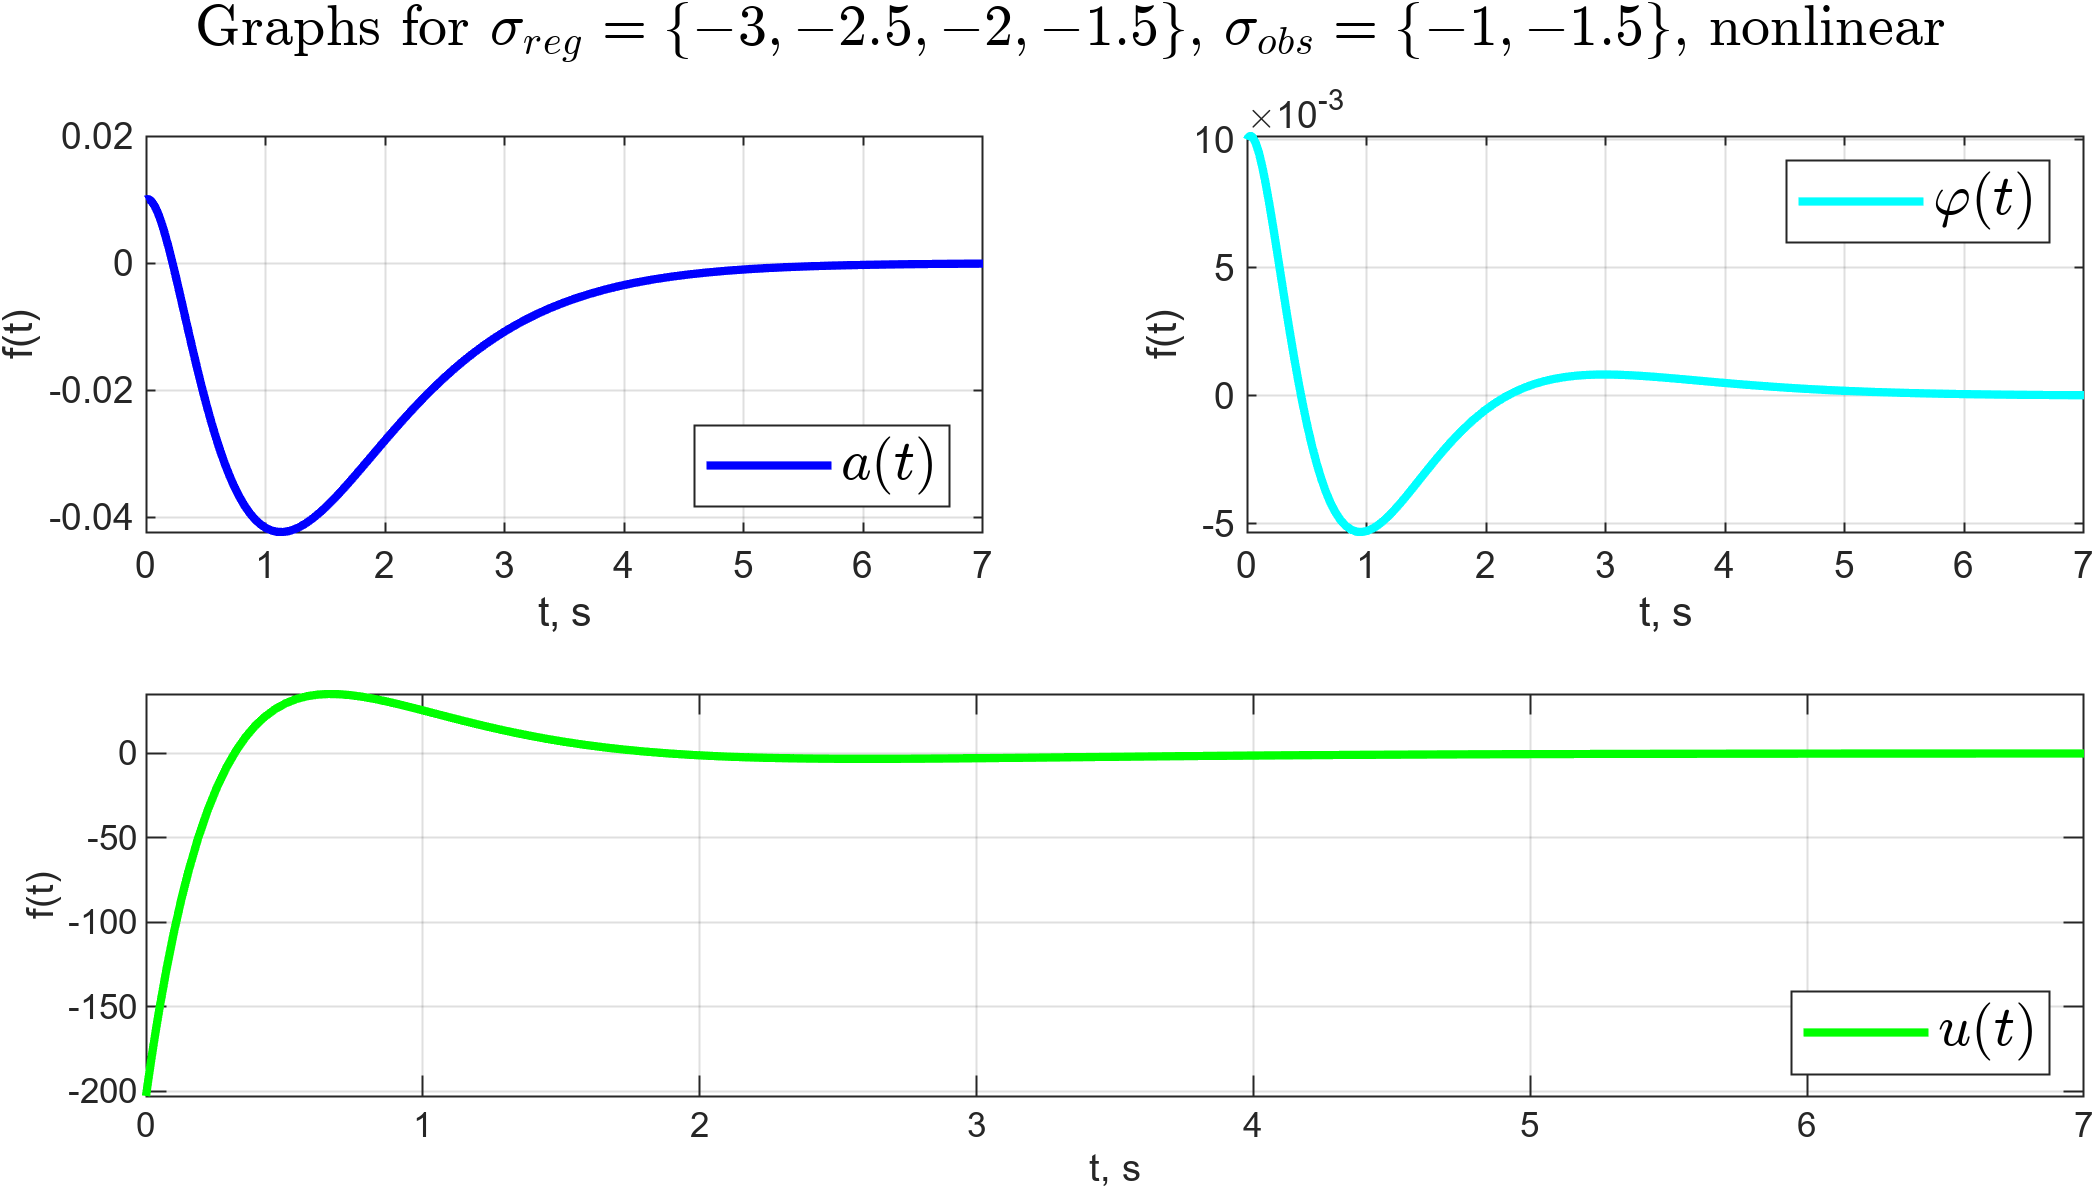
\includegraphics[width=1\linewidth]{pic/3_xu_k1l1.png}}
\caption{Графики $a(t)$, $\varphi(t)$ и $u(t)$ для $\sigma_{reg} = \{ -3, -2.5, -2, -1.5\}$, $\sigma_{obs}= \{-1, -1.5 \}$.}
\label{3_xu_k1l1}
\end{figure}

\endinput% Вторая глава
\chapter{Стабилизация маятника: регуляторы с заданной степенью устойчивости}
\label{ch:chap4}


\section{Синтез регулятора по состоянию}


С помощью решения линейного матричного неравенства Ляпунова для экспоненциальной устойчивости 
\begin{equation}
    \begin{cases}
        PA^T+AP+2 \alpha P + Y^T B^T+BY \preceq 0,\\
        K = Y P^+
    \end{cases}
\end{equation}

произведем расчет регулятора $u=Kx$, основываясь на линейной модели (\ref{1_model_lin}) и выбранной желаемой степенью устойчивости $\alpha =1 $ замкнутой системой.

\begin{equation}
    K = \begin{bmatrix}
        3064 & 4364 & -26684 & -11174
    \end{bmatrix}
\end{equation}

График вектора состояния представлен на рисунке \ref{4_1_1}.

\begin{figure}[!h]
\center{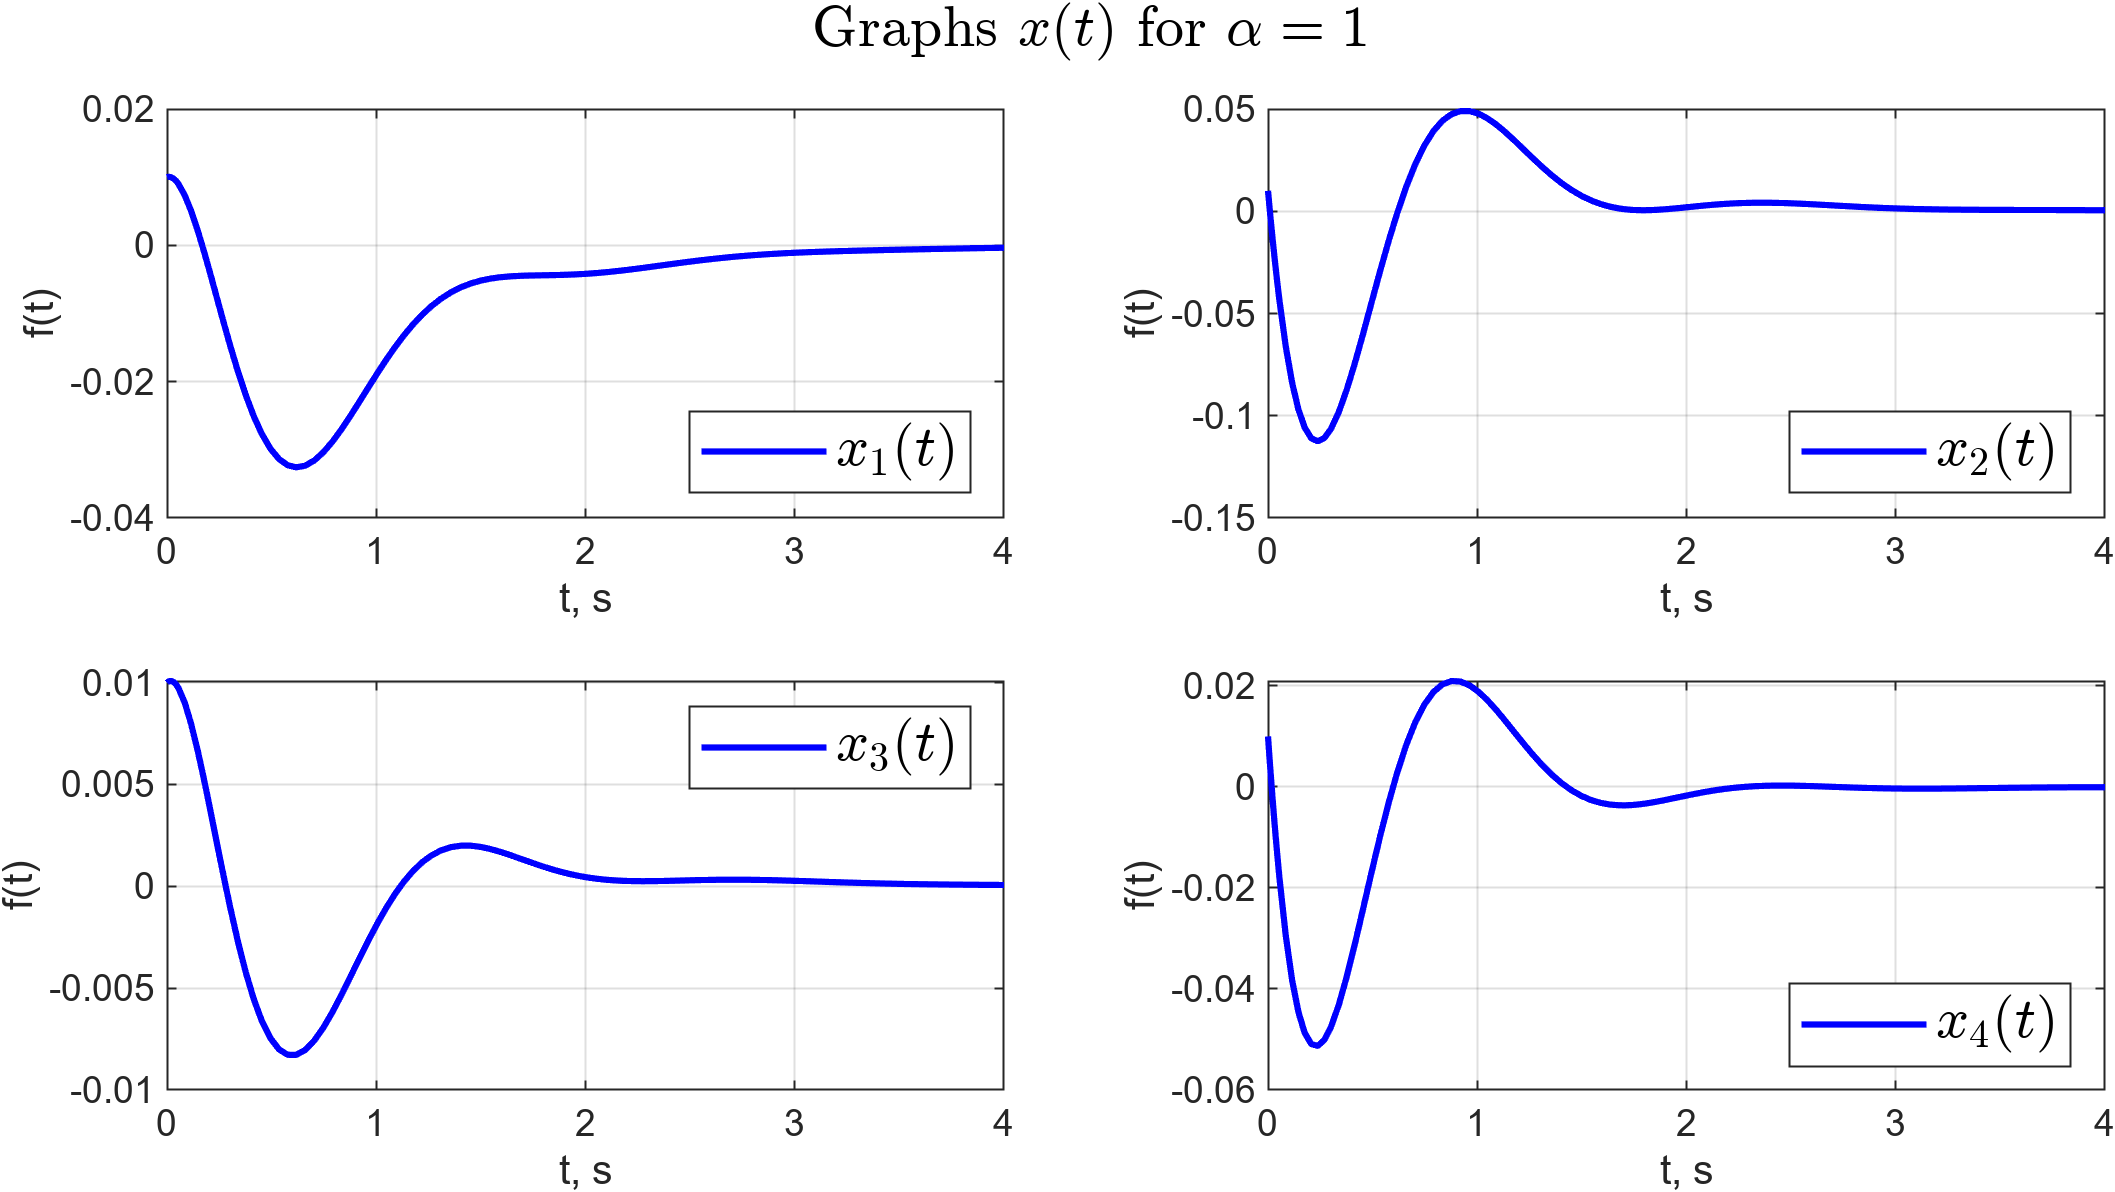
\includegraphics[width=1\linewidth]{pic/4_1_1.png}}
\caption{Графики $x(t)$, при $\alpha = 1$ и $x(0) = [0.01\, \, \,  0.01\, \, \, 0.01\, \, \, 0.01]^T$.}
\label{4_1_1}
\end{figure}






Исследуем работоспособность синтезированного регулятора при управлении нелинейной системой (\ref{1_model_full}) в зависимости от начальных условий:

\begin{equation*}
  \begin{matrix}
      x(0) = \begin{bmatrix}
          0.01 & 3 & 0.01 & 0.01
      \end{bmatrix}, & x(0) = \begin{bmatrix}
          0.01 & 0.01 & 0.01 & 1.5
      \end{bmatrix},\\
      x(0) = \begin{bmatrix}
          0.01 & 0.01 & \pi /6 & 0.01
      \end{bmatrix}, & x(0) = \begin{bmatrix}
          5 & 0.01 & 0.01 & 0.1
      \end{bmatrix},\\ 
 \end{matrix}
\end{equation*}

\begin{figure}[!h]
\center{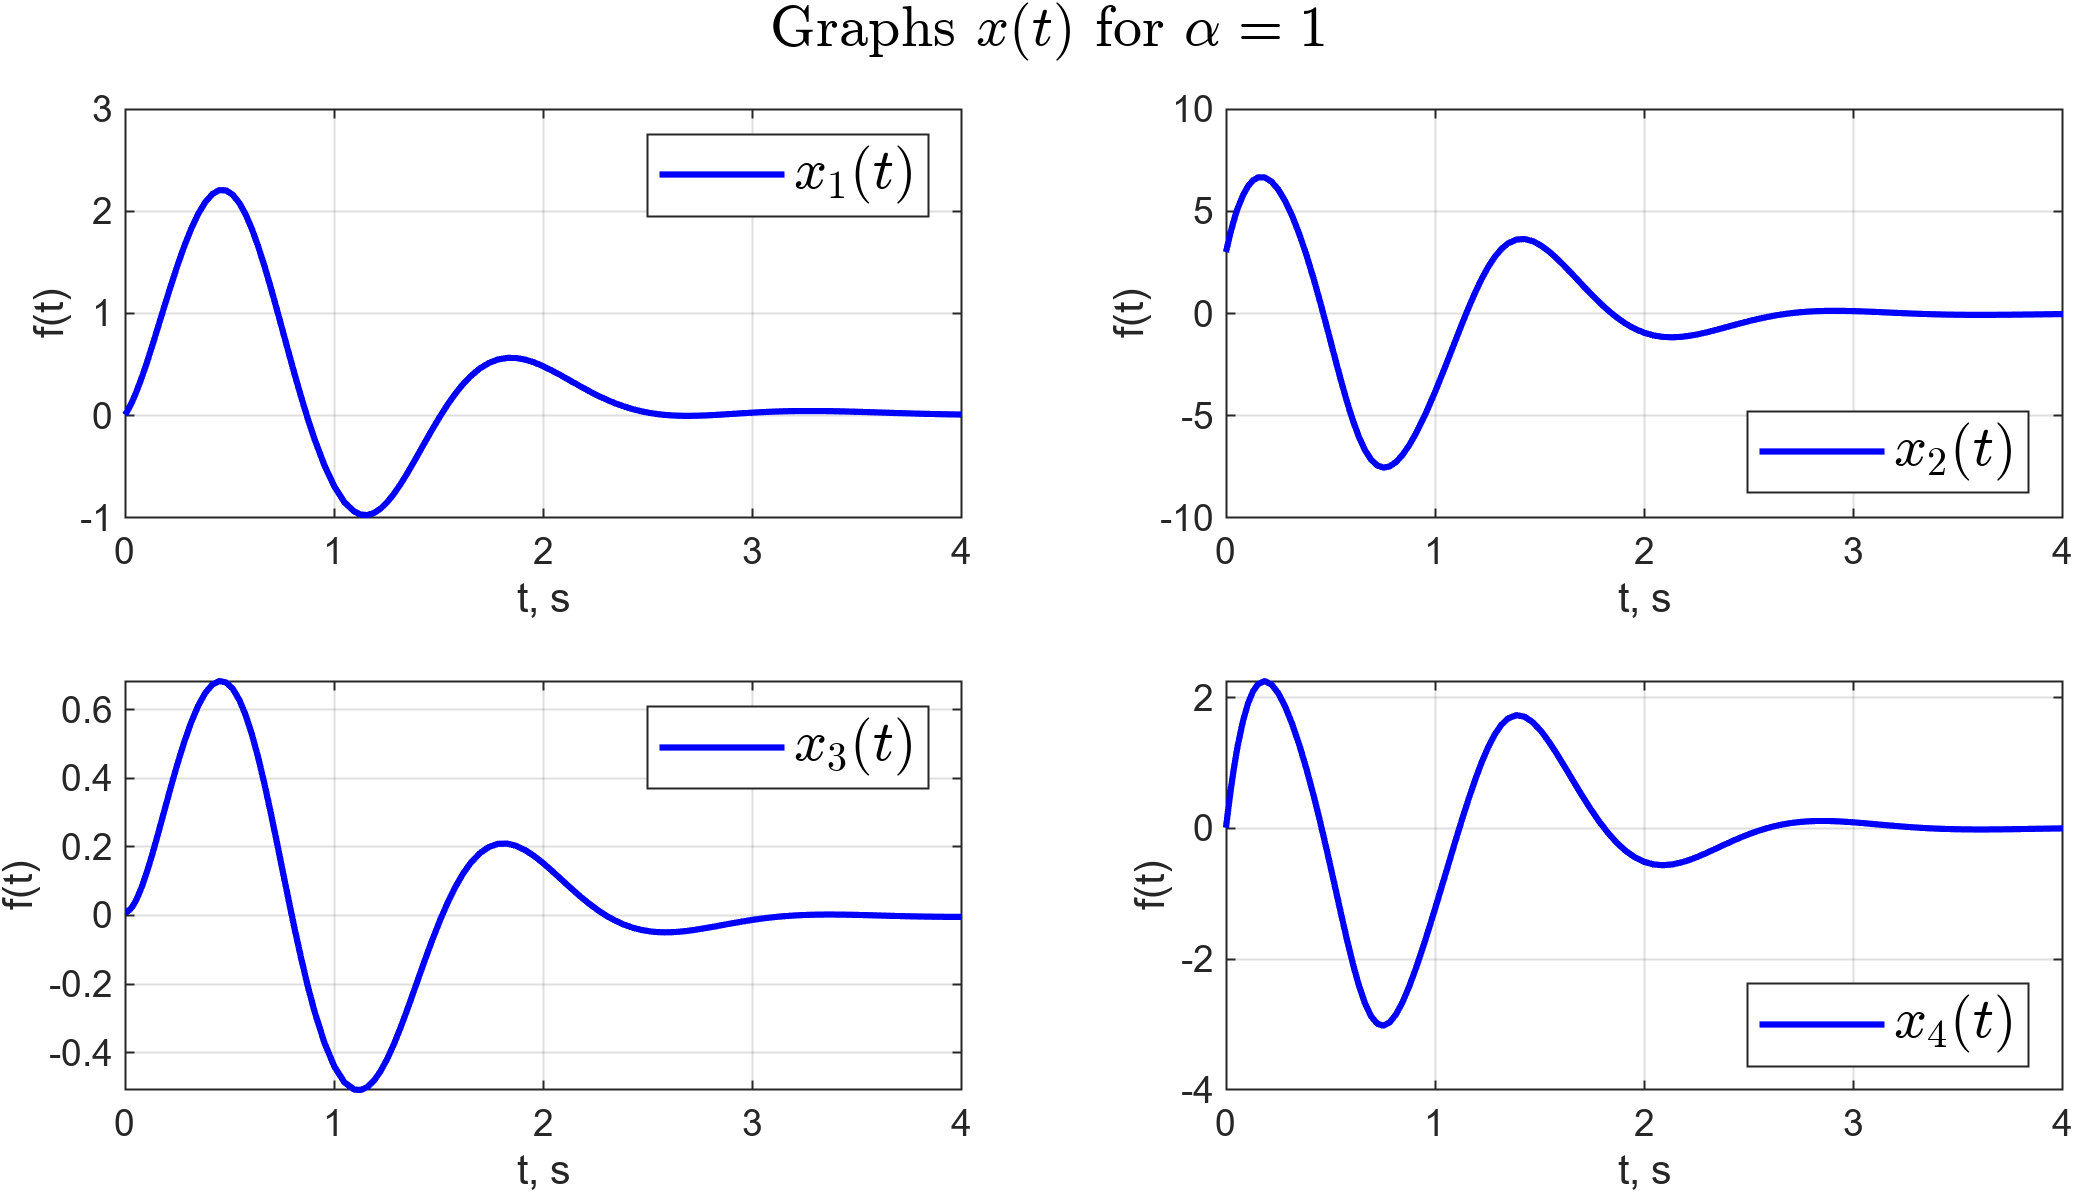
\includegraphics[width=1\linewidth]{pic/4_1_2.png}}
\caption{Графики $x(t)$, при $\alpha = 1$ и $x(0) = [0.01\, \, \,  3\, \, \, 0.01\, \, \, 0.01]^T$.}
\label{4_1_2}
\end{figure}

Заметим, что при увеличении начального значения линейной скорости до 3 м/с (рисунок \ref{4_1_2}), амплитуда компонент $x_i(t)$ возрастает примерно в 100 раз относительно начального значения 0.01 м/с.

Заметим, что при начальном значении угла отклонения маятника $\pi / 6$ регулятор еще стабилизирует систему (рисунок \ref{4_1_4}). Также видно, что для всех наборов начальных условий, вектор состояния системы становится визуально неотличим от нуля за одно и то же время $t \approx 3.5$ с. Начальные условия в данном случае влияют на амплитуду и частоту колебаний компонент вектора состояния системы.

Также начальные условия выбраны неслучайно: это максимальные значения, при которых моделирование отрабатывает за время меньше минуты -- для больших значений начальных условий не удается получить графики.

\begin{figure}[!h]
\center{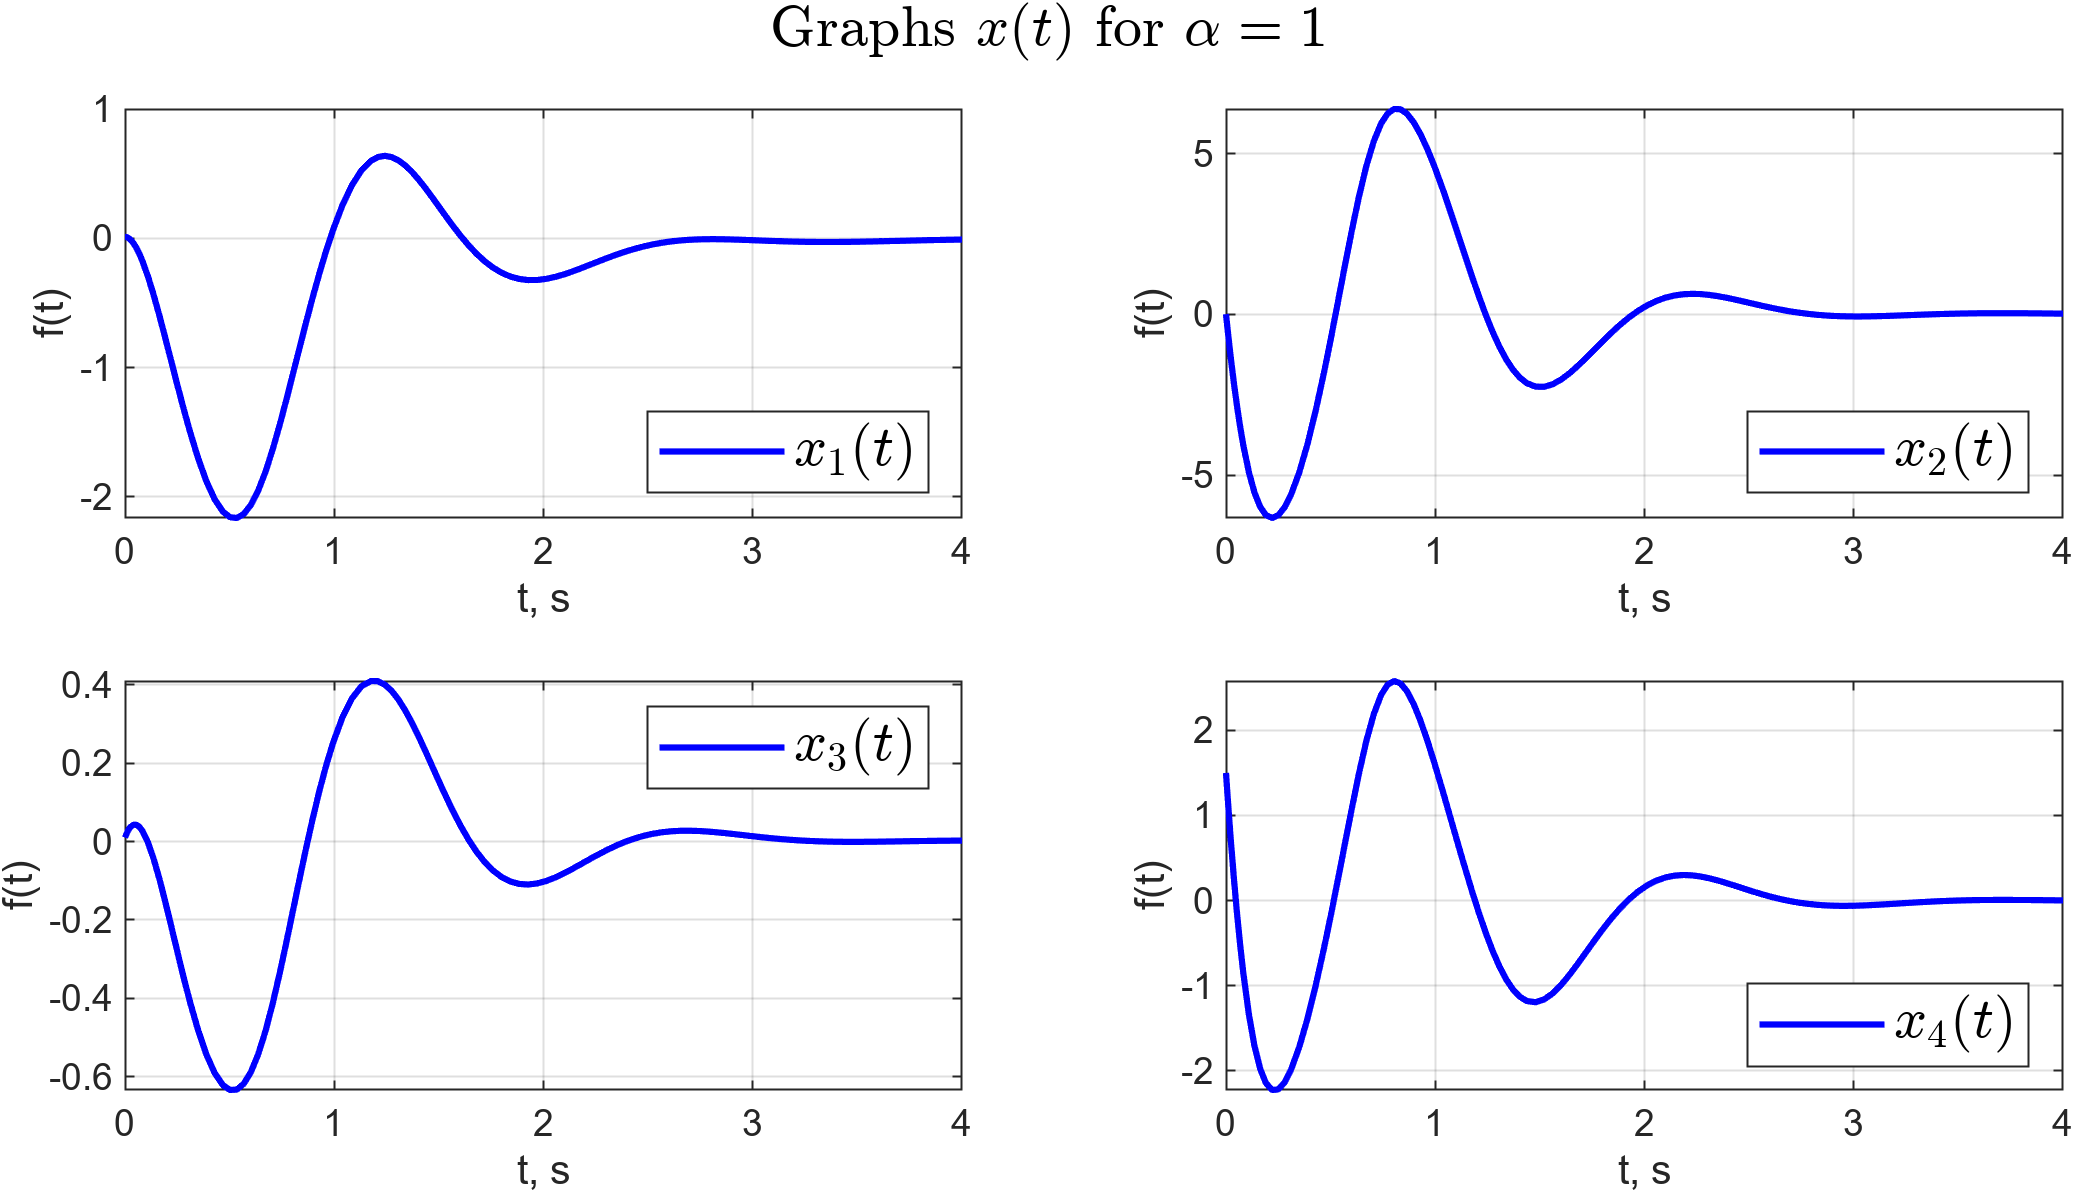
\includegraphics[width=1\linewidth]{pic/4_1_3.png}}
\caption{Графики $x(t)$, при $\alpha = 1$ и $x(0) = [0.01\, \, \,  0.01\, \, \, 0.01\, \, \, 1.5]^T$.}
\label{4_1_3}
\end{figure}


\begin{figure}[!h]
\center{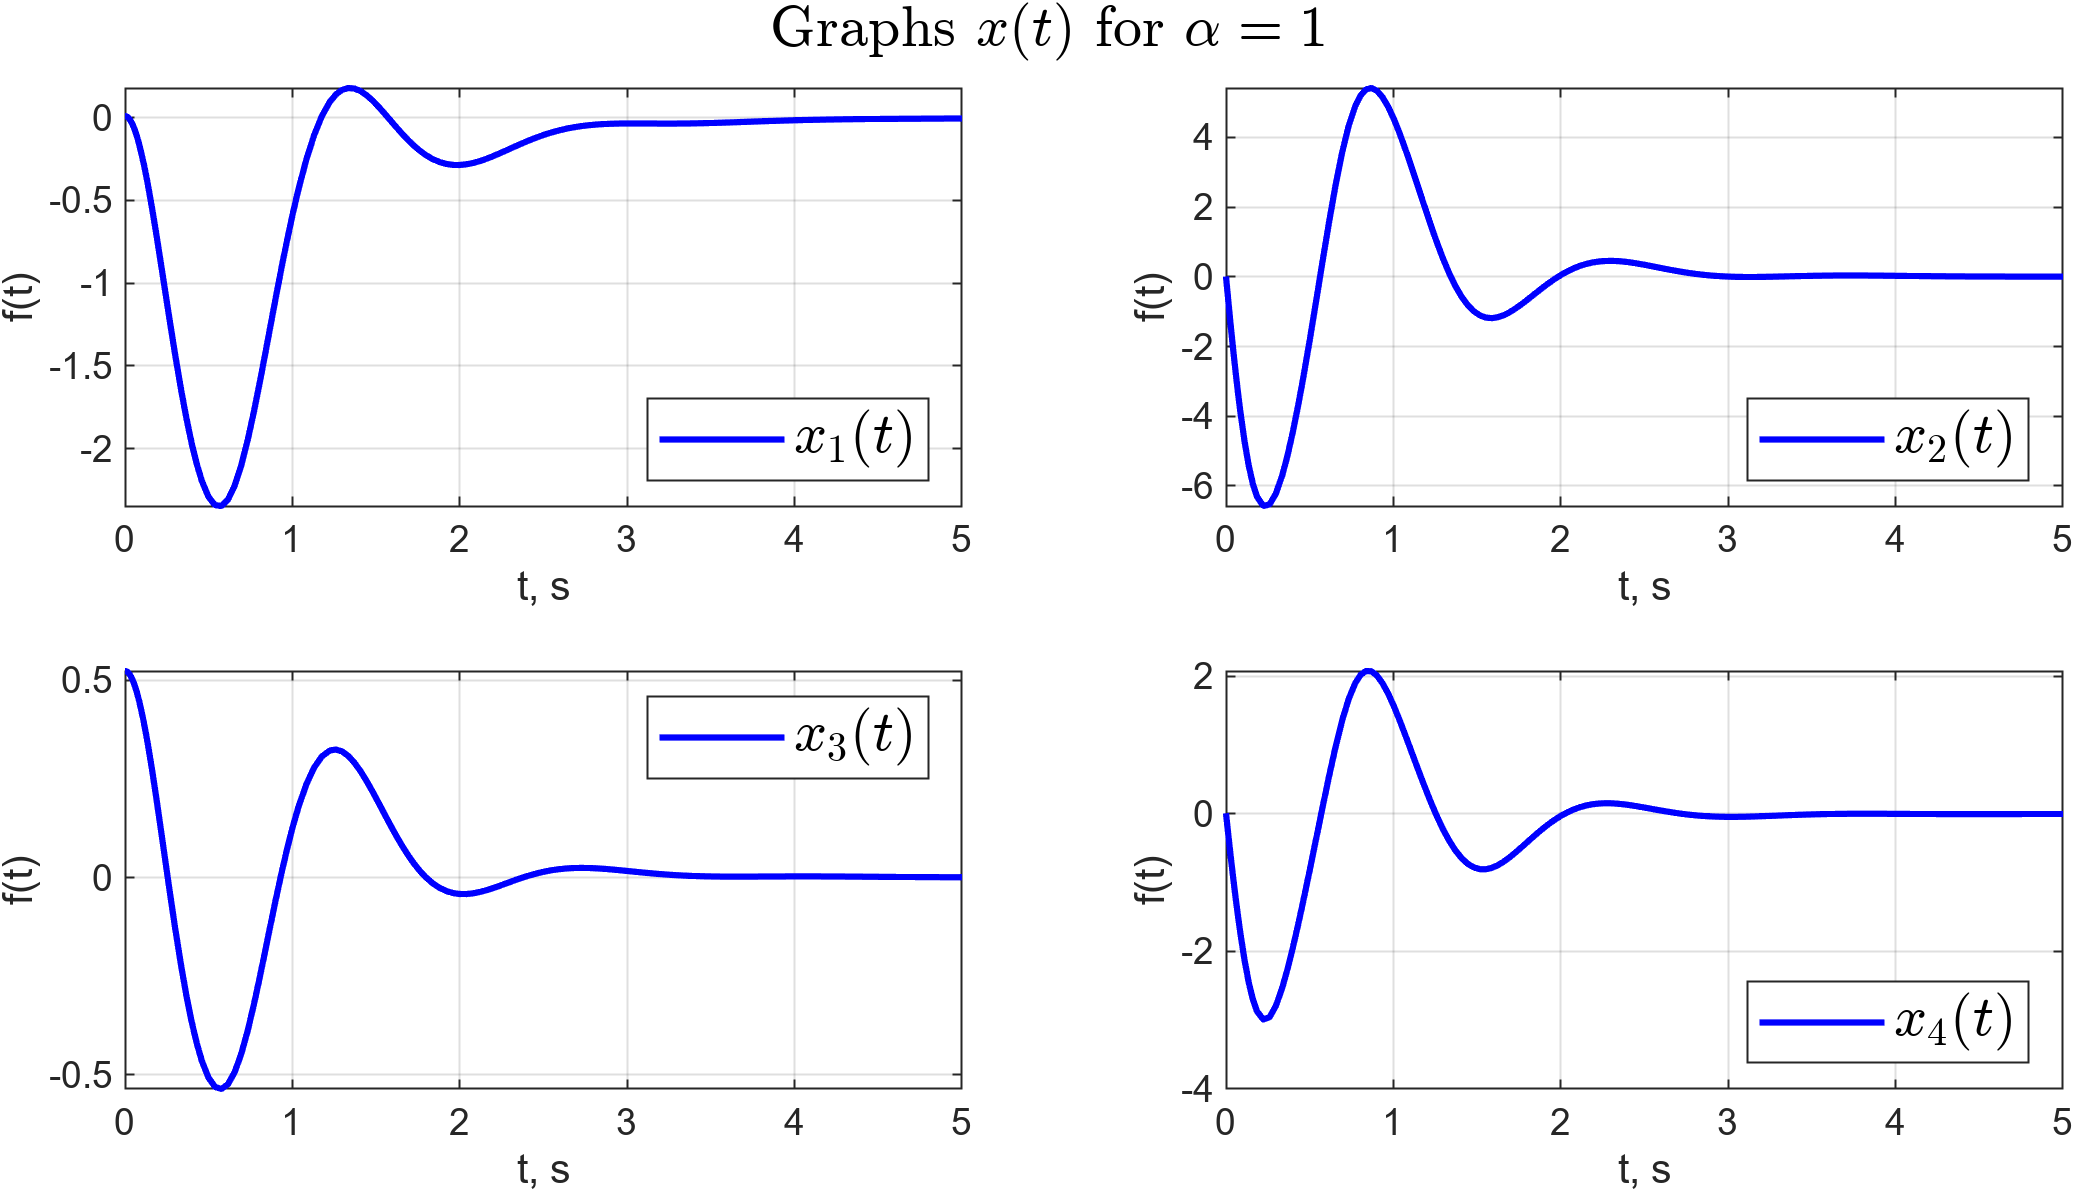
\includegraphics[width=1\linewidth]{pic/4_1_4.png}}
\caption{Графики $x(t)$, при $\alpha = 1$ и $x(0) = [0.01\, \, \,  0.01\, \, \, \pi/6\, \, \, 0.01]^T$.}
\label{4_1_4}
\end{figure}

\begin{figure}[!h]
\center{\includegraphics[width=1\linewidth]{pic/4_1_5.png}}
\caption{Графики $x(t)$, при $\alpha = 1$ и $x(0) = [5\, \, \,  0.01\, \, \, 0.01\, \, \, 0.01]^T$.}
\label{4_1_5}
\end{figure}

\section{Исследование регулятора по состоянию}

Исследуем влияние параметра $\alpha$ на максимальное отклонение маятника от вертикали, максимальное горизонтальное смещение тележки и максимальное значение управляющего сигнала при управлении нелинейной системой (\ref{1_model_full}).

 Моделирование выполнено при начальных условиях $x(0) = [0.01\, \, \,  0.01\, \, \, 0.01\, \, \, 0.01]^T$, результаты представлены в таблице \ref{4_tab_2}.


\begin{table}[h]
\centering
\caption{Результаты моделирования при разных значениях параметра $\alpha$.}
\label{4_tab_2}
\begin{tabular}{ccccc}
\toprule
$\alpha$ & $\max |\varphi|$ & $\max |a|$ & $\max |u|$ \\
\midrule
0.1  &  0.011  &  0.16  &  66  \\
0.5  &  0.01  &  0.04  &  246  \\
1 &  0.01  &  0.03  &  304  \\
2  &  0.01  &  0.025 &  942  \\
3  &  0.01  &  0.03 &  2240  \\
5  &  0.02  &  0.04 &  4732  \\
10  &  0.06  &  0.11 &  79007  \\
\bottomrule
\end{tabular}
\end{table}

Данные таблицы \ref{4_tab_2} демонстрируют сначала уменьшение максимального горизонтального смещения тележки и максимального отклонения маятника от вертикали, при $\alpha=2$ (рисунок \ref{4_2_x_2}) достигается минимум этих показателей, при дальнейшем увеличении $\alpha$ наблюдается их возрастание. Результаты моделирования представлены на рисунках \ref{4_2_x_01}-\ref{4_2_u_10}.

Максимальное значение управляющего сигнала с ростом $\alpha$ также возрастает.

\begin{figure}[!h]
	\center{\includegraphics[width=1\linewidth]{pic_fix/4_2_x_01.png}}
	\caption{Графики вектора состояния системы при $\alpha = 0.1$.}
	\label{4_2_x_01}
\end{figure}

\begin{figure}[!h]
	\center{\includegraphics[width=1\linewidth]{pic_fix/4_2_u_01.png}}
	\caption{График $u(t)$ при $\alpha = 0.1$.}
	\label{4_2_u_01}
\end{figure}

\begin{figure}[!h]
	\center{\includegraphics[width=1\linewidth]{pic_fix/4_2_x_05.png}}
	\caption{Графики вектора состояния системы при $\alpha = 0.5$.}
	\label{4_2_x_05}
\end{figure}

\begin{figure}[!h]
	\center{\includegraphics[width=1\linewidth]{pic_fix/4_2_u_05.png}}
	\caption{График $u(t)$ при $\alpha = 0.5$.}
	\label{4_2_u_05}
\end{figure}

\begin{figure}[!h]
	\center{\includegraphics[width=1\linewidth]{pic_fix/4_2_x_1.png}}
	\caption{Графики вектора состояния системы при $\alpha = 1$.}
	\label{4_2_x_1}
\end{figure}

\begin{figure}[!h]
	\center{\includegraphics[width=1\linewidth]{pic_fix/4_2_u_1.png}}
	\caption{График $u(t)$ при $\alpha = 1$.}
	\label{4_2_u_1}
\end{figure}


\begin{figure}[!h]
	\center{\includegraphics[width=1\linewidth]{pic_fix/4_2_x_2.png}}
	\caption{Графики вектора состояния системы при $\alpha = 2$.}
	\label{4_2_x_2}
\end{figure}

\begin{figure}[!h]
	\center{\includegraphics[width=1\linewidth]{pic_fix/4_2_u_2.png}}
	\caption{График $u(t)$ при $\alpha = 2$.}
	\label{4_2_u_2}
\end{figure}




\begin{figure}[!h]
	\center{\includegraphics[width=1\linewidth]{pic_fix/4_2_x_3.png}}
	\caption{Графики вектора состояния системы при $\alpha = 3$.}
	\label{4_2_x_3}
\end{figure}

\begin{figure}[!h]
	\center{\includegraphics[width=1\linewidth]{pic_fix/4_2_u_3.png}}
	\caption{График $u(t)$ при $\alpha = 3$.}
	\label{4_2_u_3}
\end{figure}


\begin{figure}[!h]
	\center{\includegraphics[width=1\linewidth]{pic_fix/4_2_x_5.png}}
	\caption{Графики вектора состояния системы при $\alpha = 5$.}
	\label{4_2_x_5}
\end{figure}

\begin{figure}[!h]
	\center{\includegraphics[width=1\linewidth]{pic_fix/4_2_u_5.png}}
	\caption{График $u(t)$ при $\alpha = 5$.}
	\label{4_2_u_5}
\end{figure}



\begin{figure}[!h]
	\center{\includegraphics[width=1\linewidth]{pic_fix/4_2_x_10.png}}
	\caption{Графики вектора состояния системы при $\alpha = 10$.}
	\label{4_2_x_10}
\end{figure}

\begin{figure}[!h]
	\center{\includegraphics[width=1\linewidth]{pic_fix/4_2_u_10.png}}
	\caption{График $u(t)$ при $\alpha = 10$.}
	\label{4_2_u_10}
\end{figure}


\section{Синтез регулятора по состоянию с ограничением на управление}

Зададимся следующими значениями параметра: $\alpha_1= 0.1$, $\alpha_2 = 0.5$, $\alpha_3 = 1$ и выполним расчет регулятора $u=Kx$ такого, чтобы наибольшее значение модуля управляющего сигнала $u$ было наименьшим из возможных, то есть при вычислении матрицы $K$ будем также решать задачу минимизации управления

\begin{equation}
    \begin{cases}
      PA^T+AP+2 \alpha P + Y^T B^T+BY \preceq 0,\\
        K = Y P^{-1}\\
        P \succ 0\\
        \begin{bmatrix}
            P & Y^T\\
            Y & \gamma
        \end{bmatrix} \succ 0\\[2pt]
        \begin{bmatrix}
            P & x(0)\\
            x^T(0) & 1
        \end{bmatrix} \succ 0
    \end{cases},
\end{equation}

Для $\alpha_1=0.1$ матрица регулятора (моделирование -- рисунок \ref{4_3_1})

\begin{equation}
    K = \begin{bmatrix}
        4.5 & 49 & -3219 & -1334
    \end{bmatrix}
\end{equation}

\begin{figure}[!h]
\center{\includegraphics[width=1\linewidth]{pic/4_3_1.png}}
\caption{Графики $x(t)$, при $\alpha = 0.1$.}
\label{4_3_1}
\end{figure}




Для $\alpha_2=0.5$ матрица регулятора (моделирование -- рисунок \ref{4_3_2})

\begin{equation}
    K = \begin{bmatrix}
        142.6 & 400.8 & -5986 & -2492
    \end{bmatrix}
\end{equation}

\begin{figure}[!h]
\center{\includegraphics[width=1\linewidth]{pic/4_3_2.png}}
\caption{Графики $x(t)$, при $\alpha = 0.5$.}
\label{4_3_2}
\end{figure}


Для $\alpha_3=1$ матрица регулятора (моделирование -- рисунок \ref{4_3_3})

\begin{equation}
    K = \begin{bmatrix}
        718& 1242 & -11091 & -4631
    \end{bmatrix}
\end{equation}

\begin{figure}[!h]
\center{\includegraphics[width=1\linewidth]{pic/4_3_3.png}}
\caption{Графики $x(t)$, при $\alpha = 1$.}
\label{4_3_3}
\end{figure}


\newpage
При увеличении значения параметра $\alpha$ увеличиваются и значения матрицы $K$, но уменьшается время переходного процесса.

Для наглядности минимизации управления составим таблицу для $\alpha_{1,2,3}$ и соответствующих значений максимального модуля управления без решения задачи минимизации и после решения задачи (таблица \ref{4_tab_3}). Заметим, что задача минимизации управления действительно выполнена.

\begin{table}[h]
\centering
\caption{Результаты моделирования при разных значениях параметра $\alpha$.}
\label{4_tab_3}
\begin{tabular}{ccc}
\toprule
$\alpha$ & $\max |u|$ & $\max |u|$ with minimization\\
\midrule
0.1  &  66  &  45  \\
0.5  &  246  &  79   \\
1 &  304  &  138 \\ 
\bottomrule
\end{tabular}
\end{table}


Исследуем работоспособность синтезированного регулятора при управлении нелинейной системой в зависимости от начальных условий


\begin{equation*}
  \begin{matrix}
      x(0) = \begin{bmatrix}
          0.01 & 3 & 0.01 & 0.01
      \end{bmatrix}^T, & x(0) = \begin{bmatrix}
          0.01 & 0.01 & 0.01 & 0.1
      \end{bmatrix}^T,\\
      x(0) = \begin{bmatrix}
          0.01 & 0.01 & \pi /16 & 0.01
      \end{bmatrix}^T, & x(0) = \begin{bmatrix}
          5 & 0.01 & 0.01 & 0.1
      \end{bmatrix}^T,\\ 
 \end{matrix}
\end{equation*}

\begin{figure}[!h]
\center{\includegraphics[width=1\linewidth]{pic/4_3_0.1_1.png}}
\caption{Графики $x(t)$, при $\alpha = 0.1$ и $x(0) = [0.01\, \, \,  3\, \, \, 0.01\, \, \, 0.01]^T$.}
\label{4_3_0.1_1}
\end{figure}


\begin{figure}[!h]
\center{\includegraphics[width=1\linewidth]{pic/4_3_0.1_2.png}}
\caption{Графики $x(t)$, при $\alpha = 0.1$ и $x(0) = [0.01\, \, \,  0.01\, \, \, 0.01\, \, \, 0.1]^T$.}
\label{4_3_0.1_2}
\end{figure}

Заметим, что значение начальной угловой скорости $0.1$ рад/с оказывается слишком большим для регулятора (рисунок \ref{4_3_0.1_2}). Кроме того, для больших значений начальной угловой скорости решения не существует. Аналогичный случай с начальным углом: максимальное значение, при котором существует решение системы $\pi /16$, здесь регулятор также не справляется с задачей стабилизации (рисунок \ref{4_3_0.1_3}).

\begin{figure}[!h]
\center{\includegraphics[width=1\linewidth]{pic/4_3_0.1_3.png}}
\caption{Графики $x(t)$, при $\alpha = 0.1$ и $x(0) = [0.01\, \, \,  0.01\, \, \, \pi /16\, \, \, 0.01]^T$.}
\label{4_3_0.1_3}
\end{figure}


\begin{figure}[!h]
\center{\includegraphics[width=1\linewidth]{pic/4_3_0.1_4.png}}
\caption{Графики $x(t)$, при $\alpha = 0.1$ и $x(0) = [5\, \, \,  0.01\, \, \, 0.01\, \, \, 0.01]^T$.}
\label{4_3_0.1_4}
\end{figure}

\newpage
Для начального условия $x(0)=\begin{bmatrix}
          0.01 & 3 & 0.01 & 0.01
      \end{bmatrix}^T$ не существует решения для $\alpha_2 = 0.5$, поэтому выполним моделирование для $x(0)=\begin{bmatrix}
          0.01 & 1 & 0.01 & 0.01
      \end{bmatrix}^T$


\begin{figure}[!h]
\center{\includegraphics[width=1\linewidth]{pic/4_3_0.5_1.png}}
\caption{Графики $x(t)$, при $\alpha = 0.5$ и $x(0) = [0.01\, \, \,  1\, \, \, 0.01\, \, \, 0.01]^T$.}
\label{4_3_0.5_1}
\end{figure}


\begin{figure}[!h]
\center{\includegraphics[width=1\linewidth]{pic/4_3_0.5_2.png}}
\caption{Графики $x(t)$, при $\alpha = 0.5$ и $x(0) = [0.01\, \, \,  0.01\, \, \, 0.01\, \, \, 0.1]^T$.}
\label{4_3_0.5_2}
\end{figure}

Заметим, что начальная угловая скорость $0.1$ рад/с, слишком большая для того, чтобы регулятор с $\alpha_2 = 0.5$ и минимальным управлением справился с задачей стабилизации (рисунок \ref{4_3_0.5_2}).

Для начального значения угла отклонения маятника $\pi /16$ также не существует решения системы неравенств, возьмем максимальный угол, при котором система имеет решение $\pi /17$, однако система расходится (рисунок \ref{4_3_0.5_3})

\begin{figure}[!h]
\center{\includegraphics[width=1\linewidth]{pic/4_3_0.5_3.png}}
\caption{Графики $x(t)$, при $\alpha = 0.5$ и $x(0) = [0.01\, \, \,  0.01\, \, \, \pi / 17\, \, \, 0.01]^T$.}
\label{4_3_0.5_3}
\end{figure}


Аналогично для начального значения координаты тележки $5$ м система неравенств не имеет решения, возьмем значение $2$ м в качестве начальной координаты тележки

\begin{figure}[!h]
\center{\includegraphics[width=1\linewidth]{pic/4_3_0.5_4.png}}
\caption{Графики $x(t)$, при $\alpha = 0.5$ и $x(0) = [2\, \, \,  0.01\, \, \, 0.01\, \, \, 0.01]^T$.}
\label{4_3_0.5_4}
\end{figure}

\newpage
Для $\alpha_3 = 1$ не существует решений системы неравенств при начальном значении линейной скорости $1$ м/с, поэтому возьмем новый вектор начальных условий $x(0) = [0.01\, \, \,  0.1\, \, \, 0.01\, \, \, 0.01]^T$

\begin{figure}[!h]
\center{\includegraphics[width=1\linewidth]{pic/4_3_1_1.png}}
\caption{Графики $x(t)$, при $\alpha = 1$ и $x(0) = [0.01\, \, \,  0.1\, \, \, 0.01\, \, \, 0.01]^T$.}
\label{4_3_1_1}
\end{figure}

Для второго вектора начальных условий (с большим значением угловой скорости) тоже выберем вектор с меньшим значением угловой начальной скорости, потому что при $1$ рад/с для $\alpha_3 = 1$ также не удается найти решение системы, новый вектор: $x(0) = [0.01\, \, \,  0.01\, \, \, 0.01\, \, \, 0.1]^T$

\begin{figure}[!h]
\center{\includegraphics[width=1\linewidth]{pic/4_3_1_2.png}}
\caption{Графики $x(t)$, при $\alpha = 1$ и $x(0) = [0.01\, \, \,  0.01\, \, \, 0.01\, \, \, 0.1]^T$.}
\label{4_3_1_2}
\end{figure}


\begin{figure}[!h]
\center{\includegraphics[width=1\linewidth]{pic/4_3_1_3.png}}
\caption{Графики $x(t)$, при $\alpha = 1$ и $x(0) = [0.01\, \, \,  0.01\, \, \, \pi / 60\, \, \, 0.01]^T$.}
\label{4_3_1_3}
\end{figure}


\begin{figure}[!h]
\center{\includegraphics[width=1\linewidth]{pic/4_3_1_4.png}}
\caption{Графики $x(t)$, при $\alpha = 1$ и $x(0) = [0.05\, \, \,  0.01\, \, \, 0.01\, \, \, 0.01]^T$.}
\label{4_3_1_4}
\end{figure}

\newpage
С ростом значения $\alpha$ существенно сужалась область допустимых начальных условий, при которых система матричных неравенств имеет решение.

\section{Исследование регулятора по состоянию с ограничением на управление}

Исследуем влияние параметра $\alpha$ на максимальное отклонение маятника от вертикали, максимальное горизонтальное смещение тележки и максимальное значение сигнала при управлении нелинейной системой (\ref{1_model_full}), результаты представим в таблице \ref{4_tab_4}


\begin{table}[h]
\centering
\caption{Результаты моделирования при разных значениях параметра $\alpha$.}
\label{4_tab_4}
\begin{tabular}{ccccc}
\toprule
$\alpha$ & $\max |\varphi|$ & $\max |a|$ & $\max |u|$ \\
\midrule
0.1  &  0.012  &  0.51  &  45 \\
0.5  &  0.01  &  0.09  &   79 \\
1 &  0.01  &  0.05  &  138  \\
2  &  13946  &  2879 &   46 \\
\bottomrule
\end{tabular}
\end{table}

В таблице \ref{4_tab_4} для $\alpha=2$ указаны значения, полученные в результате моделирования, истинные значения параметров стремятся к бесконечности с ростом времени моделирования.

До значения $\alpha=2$ (не включительно) мы видим снижение таких параметров как максимальное отклонение маятника от вертикали и максимальное горизонтальное смещение тележки. Также с ростом $\alpha$ мы наблюдаем рост максимального значения управляющего сигнала. При $\alpha=2$ регулятор не обеспечивает стабилизацию системы, поэтому мы получаем большие значения угла, координаты. Результаты моделирования представлены на рисунках \ref{4_4_x_01}-\ref{4_4_u_2}.

% alpha = 0.1
\begin{figure}[!h]
	\center{\includegraphics[width=1\linewidth]{pic_fix/4_4_x_01.png}}
	\caption{Графики вектора состояния системы при $\alpha = 0.1$.}
	\label{4_4_x_01}
\end{figure}

\begin{figure}[!h]
	\center{\includegraphics[width=1\linewidth]{pic_fix/4_4_u_01.png}}
	\caption{График $u(t)$ при $\alpha = 0.1$.}
	\label{4_4_u_01}
\end{figure}


% alpha = 0.5
\begin{figure}[!h]
	\center{\includegraphics[width=1\linewidth]{pic_fix/4_4_x_05.png}}
	\caption{Графики вектора состояния системы при $\alpha = 0.5$.}
	\label{4_4_x_05}
\end{figure}

\begin{figure}[!h]
	\center{\includegraphics[width=1\linewidth]{pic_fix/4_4_u_05.png}}
	\caption{График $u(t)$ при $\alpha = 0.5$.}
	\label{4_4_u_05}
\end{figure}



% alpha = 1
\begin{figure}[!h]
	\center{\includegraphics[width=1\linewidth]{pic_fix/4_4_x_1.png}}
	\caption{Графики вектора состояния системы при $\alpha = 1$.}
	\label{4_4_x_1}
\end{figure}

\begin{figure}[!h]
	\center{\includegraphics[width=1\linewidth]{pic_fix/4_4_u_1.png}}
	\caption{График $u(t)$ при $\alpha = 1$.}
	\label{4_4_u_1}
\end{figure}


% alpha = 2
\begin{figure}[!h]
	\center{\includegraphics[width=1\linewidth]{pic_fix/4_4_x_2.png}}
	\caption{Графики вектора состояния системы при $\alpha = 2$.}
	\label{4_4_x_2}
\end{figure}

\begin{figure}[!h]
	\center{\includegraphics[width=1\linewidth]{pic_fix/4_4_u_2.png}}
	\caption{График $u(t)$ при $\alpha = 2$.}
	\label{4_4_u_2}
\end{figure}



\section{Синтез наблюдателя}
С помощью решения линейного матричного неравенства Ляпунова для экспоненциальной устойчивости произведем расчет наблюдателя полной размерности
$\dot{\hat{x}} = A\hat{x} + Bu + L(\hat{y} - y)$
основываясь на линейной модели (\ref{1_model_lin}) и выбранной степени сходимости $\alpha = 1.2$ динамики ошибки наблюдателя.

\begin{equation}
    \begin{cases}
        A^T Q +QA+2 \alpha Q + C^TY^T+YC \preceq 0,\\
        L = Q^{-1}Y
    \end{cases}
\end{equation}

После решения системы получим

\begin{equation}
    L = \begin{bmatrix}
        -9.8432	&-0.4422\\
-23.3319	&-1.2561\\
0.4422	&-9.8432\\
1.0032	&-29.1714
    \end{bmatrix}
\end{equation}




\section{Синтез регулятора по выходу}

На основе линейных матричных неравенств построим регулятор, стабилизирующий маятник и тележку в условиях, когда измерению доступны только сигналы $y_1$, $y_2$.

Зададимся значениями степеней устойчивости: $\alpha_K = 0.5$ -- для регулятора и $\alpha_L=1.2$ -- для наблюдателя и проведем компьютерное моделирование с нулевыми начальными условиями наблюдателя и $x(0) = \begin{bmatrix}
    0.01 & 0.01 & 0.01 & 0.01
\end{bmatrix}^T$ -- начальными условиями вектора состояния системы. Результаты моделирования представлены на рисунках \ref{4_6_1.20.5x} и \ref{4_6_1.20.5e}.

\begin{figure}[!h]
	\center{\includegraphics[width=1\linewidth]{pic/4_6_1.20.5x.png}}
	\caption{Графики $\hat{x}(t)$ и $x(t)$, при $\alpha_L = 1.2$ и $\alpha_K = 0.5$.}
	\label{4_6_1.20.5x}
\end{figure}

\begin{figure}[!h]
	\center{\includegraphics[width=1\linewidth]{pic/4_6_1.20.5e.png}}
	\caption{Графики $e(t) = \hat{x}(t)-x(t)$, при $\alpha_L = 1.2$ и $\alpha_K = 0.5$.}
	\label{4_6_1.20.5e}
\end{figure}

\newpage
Проведем исследование работоспособности построенного регулятора при управлении нелинейной системой (\ref{1_model_full}) в зависимости от выбранных степеней устойчивости. Зададимся наборами степеней устойчивости (таблица \ref{4_tab_6}) и выполним моделирование (рисунки \ref{4_6_0.50.5x}-\ref{4_6_55e}). Время  переходного процесса $t$ (как последний момент времени, когда координата тележки или угол отклонения маятника отличался от нуля более, чем на 0.001), время $t_e$ -- последний момент времени, когда ошибка координаты тележки или угла отклонения маятника  отличался от нуля более, чем на 0.001.

\begin{table}[!h]
	\centering
	\caption{Результаты моделирования при разных значениях параметров $\alpha_K$ и $\alpha_L$.}
	\label{4_tab_6}
	\begin{tabular}{ccccccc}
		\toprule
		$\alpha_K$ & $\alpha_L$ & $\max |\varphi|$ & $\max |a|$  & $t_e$ & $t$ \\
		\midrule
		0.5  &  0.5  &  0.011  &  0.085 & 3.35 & 8.16  \\
		0.5  &  5  &  0.01  &  0.03 & 0.41 & 5.78  \\
		5 &  0.5  &  0.01  &  0.03 & 3.34 & 5.49   \\
		5  &  5  &  0.04  &  0.08 & 0.42 & 1.64 \\
		\bottomrule
	\end{tabular}
\end{table}




\begin{figure}[!h]
\center{\includegraphics[width=1\linewidth]{pic/4_6_0.50.5x.png}}
\caption{Графики $\hat{x}(t)$ и $x(t)$, при $\alpha_L = 0.5$ и $\alpha_K = 0.5$.}
\label{4_6_0.50.5x}
\end{figure}

\begin{figure}[!h]
\center{\includegraphics[width=1\linewidth]{pic/4_6_0.50.5e.png}}
\caption{Графики $e(t) = \hat{x}(t)-x(t)$, при $\alpha_L = 0.5$ и $\alpha_K = 0.5$.}
\label{4_6_0.50.5e}
\end{figure}


\begin{figure}[!h]
\center{\includegraphics[width=1\linewidth]{pic/4_6_50.5x.png}}
\caption{Графики $\hat{x}(t)$ и $x(t)$, при $\alpha_L = 5$ и $\alpha_K = 0.5$.}
\label{4_6_50.5x}
\end{figure}

\begin{figure}[!h]
\center{\includegraphics[width=1\linewidth]{pic/4_6_50.5e.png}}
\caption{Графики $e(t) = \hat{x}(t)-x(t)$, при $\alpha_L = 5$ и $\alpha_K = 0.5$.}
\label{4_6_50.5e}
\end{figure}


\begin{figure}[!h]
\center{\includegraphics[width=1\linewidth]{pic/4_6_0.55x.png}}
\caption{Графики $\hat{x}(t)$ и $x(t)$, при $\alpha_L = 0.5$ и $\alpha_K = 5$.}
\label{4_6_0.55x}
\end{figure}

\begin{figure}[!h]
\center{\includegraphics[width=1\linewidth]{pic/4_6_0.55e.png}}
\caption{Графики $e(t) = \hat{x}(t)-x(t)$, при $\alpha_L = 0.5$ и $\alpha_K = 5$.}
\label{4_6_0.55e}
\end{figure}


\begin{figure}[!h]
\center{\includegraphics[width=1\linewidth]{pic/4_6_55x.png}}
\caption{Графики $\hat{x}(t)$ и $x(t)$, при $\alpha_L = 5$ и $\alpha_K = 5$.}
\label{4_6_55x}
\end{figure}

\begin{figure}[!h]
\center{\includegraphics[width=1\linewidth]{pic/4_6_55e.png}}
\caption{Графики $e(t) = \hat{x}(t)-x(t)$, при $\alpha_L = 5$ и $\alpha_K = 5$.}
\label{4_6_55e}
\end{figure}

\newpage
\,
\newpage
\,
\newpage
\,
\newpage
Как можно заметить для различных комбинаций значений степеней устойчивости $0.5$ и $5$ регулятор по выходу справляется с задачей стабилизации. Чем выше $\alpha_L$, тем быстрее ошибка между $\hat{x}(t)$ и $x(t)$ сходится к нулю ($0.41$-$0.42$ секунды для $\alpha_L= 5$ и $3.34$-$3.35$ секунды для $\alpha_L= 0.5$), сочетание большого значения $\alpha_{L,K}=5$ приводит к меньшему времени стабилизации системы, но к большей аплитуде координаты тележки и угла отклонения маятника от вертикали.


\endinput
\chapter{Слежение и компенсация}
\label{ch:chap5}

\section{Решение задачи компенсации}
Зададим сигнал $f$ в модели
\begin{equation}
    \begin{cases}
       \dot{x} = Ax + Bu + Df,\\
     y=Cx,  
    \end{cases}
\end{equation}

виде суммы гармоник

\begin{equation}
    f(t) = \sum \limits_{k=1}^5 A_k \sin(\omega_kt+\phi_k),
\end{equation}
где
\begin{equation}
    \begin{matrix}
        A_1 = 1, & \omega_1 = 0.5, & \phi_1 = 0\\
        A_2 = 0.8, & \omega_2 = 1, & \phi_2 = \pi /4\\
        A_3 = 0.6, & \omega_3 = 1.5, & \phi_3 = \pi /3\\
        A_4 = 0.4, & \omega_4 = 2, & \phi_4 = -\pi/4\\
        A_5= 0.2, & \omega_5 = 2.5, & \phi_5 = \pi / 6\\
    \end{matrix}
\end{equation}

Построим компенсирующий регулятор, гарантирующий выполнение условия

\begin{equation}
\label{5_goal_1}
    \lim \limits_{t \to \infty} \| \varphi(t) \| = 0,
\end{equation}



Запишем возмущение $f$ через генератор

\begin{equation}
    \begin{cases}
        \dot{w} = \Gamma_f w\\
        f = Y_fw
    \end{cases}
\end{equation}
Теперь нам необходимо определить значения $\Gamma_f$, $Y_f$ и $w(0)$

\begin{multline}
    \Gamma_f = block \,diag \left( 
    \begin{bmatrix}
        0 & -w_1\\
        w_1 & 0
    \end{bmatrix}\dots 
    \begin{bmatrix}
        0 & -w_5\\
        w_5 & 0
    \end{bmatrix}
    \right) =\\[2ex]
    = \begin{bmatrix}
        0 & -0.5 & 0 & 0 & 0 & 0 & 0 & 0&0&0\\
        0.5 & 0 & 0 & 0 & 0 & 0 & 0 & 0&0&0\\
        0 & 0 & 0 & -1 & 0 & 0 & 0 & 0&0&0\\
        0 & 0 & 1 & 0 & 0 & 0 & 0 & 0&0&0\\
        0 & 0 & 0 & 0 & 0 & -1.5 & 0 & 0&0&0\\
        0 & 0 & 0 & 0 & 1.5 & 0 & 0 & 0&0&0\\
        0 & 0 & 0 & 0 & 0 & 0 & 0 & -2&0&0\\
        0 & 0 & 0 & 0 & 0 & 0 & 2 & 0&0&0\\
        0 & 0 & 0 & 0 & 0 & 0 & 0 & 0&0&-2.5\\
        0 & 0 & 0 & 0 & 0 & 0 & 0 & 0&2.5&0
    \end{bmatrix} 
\end{multline}

При переходе к матричной экспоненте $e^{\Gamma_f t}$ каждый блок 

\begin{equation}\begin{bmatrix}
        0 & -w_i\\
        w_i & 0
\end{bmatrix}\end{equation}
перейдет в 
\begin{equation}\begin{bmatrix}
        \cos (w_it) & -\sin (w_it)\\
        \sin (w_it) & \cos (w_it)
\end{bmatrix}
\end{equation}
    
Запишем $f(t)$ и упростим его компоненты
\begin{multline}
    f(t) = \sin (0.5t) + 0.8 \sin(t+\pi/4)+ 0.6 \sin (1.5 t+ \pi/3)+\\+0.4 sin(2t-\pi/4) + 0.2\sin(2.5t+\pi/6) =\sin (0.5t)+ 0.4\sqrt{2} \sin{t} +\\+ 0.4\sqrt{2} \cos{t} + 0.3 \sin(1.5t)+
    0.3 \sqrt{3} \cos(1.5t) + 0.2 \sqrt{2} \sin(2t) - \\-0.2\sqrt{2}\cos(2t) + 0.1 \sqrt{3} \sin(2.5t) + 0.1 \cos(2.5t)
\end{multline}
Основываясь на следующей системе уравнений, найдем подходящие значения $w(0)$ и $Y_f$

\begin{equation}
\begin{cases}
    w = e^{\Gamma_f t} w(0)\\
    f = Y_f e^{\Gamma_f t} w(0)
\end{cases}
\end{equation}

\begin{equation}
    w(0) = \begin{bmatrix}
       1 &  0 & 1 & 0 & 1 & 0 & 1 & 0 & 1 & 0
    \end{bmatrix}^T
\end{equation}

\begin{equation}
    Y_f = \begin{bmatrix}
        0 & 1 & 0.4\sqrt{2} & 0.4\sqrt{2} & 0.3\sqrt{3} & 0.3 & -0.2 \sqrt{2} & 0.2 \sqrt{2} & 0.1 & 0.1 \sqrt{3}
    \end{bmatrix}
\end{equation}

Запишем общий вид необходимого регулятора

\begin{equation}
    u = Kx + K_f w
\end{equation}

В качестве $K$ возьмем ранее вычисленный в пункте 4.1 регулятор 
\begin{equation}
    K = \begin{bmatrix}
        3064 & 4364 & -26684 & -11174
    \end{bmatrix}
\end{equation}

теперь нам необходимо вычислить компенсирующую компоненту $K_f$ регулятора. Запишем систему матричных уравнений Франкиса-Дэвисона

\begin{equation}
\label{5_fran_f}
    \begin{cases}
       P_f \Gamma_f - (A+BK)P_f-DY_f=BK_f\\
       CP_f = 0
    \end{cases}
\end{equation}

Проверим условие существования решения системы уравнений (\ref{5_fran_f}).

Решение относительно $P_f$ и $K_f$ есть, если

\begin{equation}
\label{5_f_rule}
    rank \begin{bmatrix}
        A+BK-I\lambda_{i\Gamma_f}&B\\
        C & 0
    \end{bmatrix} = \text{число строк}
\end{equation}

В ходе проверки этого условия было выяснено, что ранг искомых матриц равен 5, что меньше числа строк в матрицах, 6. От нас требуется компенсировать только значение угла (\ref{5_goal_1}), то есть $y_2(t) = \varphi(t)$. Будем работать с матрицей $\tilde{C}$ вместо $C$

\begin{equation}
    C = \begin{bmatrix}
        1 & 0 & 0 & 0\\
        0 & 0 & 1 & 0
    \end{bmatrix} \Rightarrow 
    \tilde{C} =\begin{bmatrix}
        0 & 0 & 1 & 0
    \end{bmatrix} 
\end{equation}

Вновь проверим, условие (\ref{5_f_rule}) только теперь вместо матрицы $C$ будем использовать $\tilde{C}$. Условие существования решения выполнено ранг каждой исследованной матрицы равен 5, что совпадает с количеством строк в матрицах.

В результате решения системы (\ref{5_fran_f}) получим значение компенсирующей компоненты регулятора

\begin{equation}
    K_f = \begin{bmatrix}
        -736.0530	\\-1056.7\\-367.4171	\\48.9573	\\-145.2753	\\86.1095	\\-27.2456	\\-76.8480	\\-31.9406	\\3.5614
    \end{bmatrix}^T
\end{equation}

Проведем моделирование для линейной модели 

\begin{figure}[!h]
\center{\includegraphics[width=1\linewidth]{pic2/5_f_lin.png}}
\caption{Графики выходного сигнала $y(t)$ и внешнего воздействия $f(t)$ для линейной системы.}
\label{5_f_lin}
\end{figure}

Заметим, что целевое условие (\ref{5_goal_1}) действительно выполнено, компонента выхода $y_2(t) = \varphi(t)$ сходится к нулю с течение времени. Задача компенсации для линейной системы выполнена.

Исследуем поведение регулятора для нелинейного случая.

\begin{figure}[!h]
\center{\includegraphics[width=1\linewidth]{pic2/5_f_nonlin.png}}
\caption{График выходного сигнала $y(t)$ для нелинейной системы при $x(0) = 
    [0.01 \,\, 0.01 \,\, 0.01 \,\, 0.01]^T$.}
\label{5_f_nonlin}
\end{figure}

Для нелинейного случая при начальных условиях системы $x(0) = \begin{bmatrix}
    0.01 & 0.01 & 0.01 & 0.01
\end{bmatrix}^T$ синтезированный компенсирующий регулятор так же справляется с задачей (рисунок \ref{5_f_nonlin}).

\begin{figure}[!h]
\center{\includegraphics[width=1\linewidth]{pic2/5_f_nonlin_1.png}}
\caption{График выходного сигнала $y(t)$ для нелинейной системы при $x(0) = 
    [0.01 \,\, 0.01 \,\, 0.5 \,\, 0.01]^T$.}
\label{5_f_nonlin_1}
\end{figure}

При увеличении начального значения угла отклонения амплитуда $y_2(t)$ и время, за которое он сходится к нулю возрастает (рисунок \ref{5_f_nonlin_1}). Кроме того, не удается получить результаты моделирования при задании больших значений начального угла  за ограниченное время.





\section{Решение задачи слежения}

Пусть $f=0$. Зададимся целевым сигналом $g(t)$, который описывает желаемое поведение $\varphi (t)$

\begin{equation}
	g(t) = \sum \limits_{k=1}^5 A_k \sin(\omega_kt+\phi_k),
\end{equation}
где
\begin{equation}
	\begin{matrix}
		A_1 = 1, & \omega_1 = 0.5, & \phi_1 = 0\\
		A_2 = 0.8, & \omega_2 = 1, & \phi_2 = \pi /4\\
		A_3 = 0.6, & \omega_3 = 1.5, & \phi_3 = \pi /3\\
		A_4 = 0.4, & \omega_4 = 2, & \phi_4 = -\pi/4\\
		A_5= 0.2, & \omega_5 = 2.5, & \phi_5 = \pi / 6\\
	\end{matrix}
\end{equation}

Построим следящий регулятор, гарантирующий выполнение условия

\begin{equation}
	\lim \limits_{t\to \infty} \| \varphi (t) - g(t) \| = 0
\end{equation}

Запишем целевой сигнал $g$ через генератор

\begin{equation}
\begin{cases}
	\dot{w}_g = \Gamma_g w_g\\
	g = Y_g w_g
\end{cases}
\end{equation}

Значения матриц $\Gamma_g$, $Y_g$, $w_g(0)$ совпадают соответственно с $\Gamma_f$, $Y_f$, $w(0)$, так как сигналы $g(t)$ и $f(t)$ одинаковы.

Необходимый регулятор будет иметь вид

\begin{equation}
	u = Kx + K_g w_g
\end{equation}

Стабилизирующую компоненту $K$ выберем такой же как и в прошлом пункте. 
Запишем систему уравнений Франкиса-Дэвисона

\begin{equation}
	\begin{cases}
		P_g \Gamma_g - (A+BK) P_g = BK_g\\
		CP_g = Y_g
	\end{cases}
\end{equation}

Условие существование здесь будет то же, что и в прошлом пункте.

Синтезируем матрицу следящей компоненты регулятора

\begin{equation}
	K_g = \begin{bmatrix}
		-83795\\	-101630\\	-28825\\	15476\\	-4671\\	13280\\	-6636.1\\	-1338.9\\	-280.4743\\	2710.3
	\end{bmatrix}^T
\end{equation}

И выполним моделирование для линейной системы

\begin{figure}[!h]
	\center{\includegraphics[width=1\linewidth]{pic2/5_g_lin.png}}
	\caption{Графики выходного сигнала $y_2(t)$ и задающего сигнала $g(t)$ для линейной системы.}
	\label{5_g_lin}
\end{figure}

\begin{figure}[!h]
	\center{\includegraphics[width=1\linewidth]{pic2/5_e_lin.png}}
	\caption{График ошибки слежения $e(t) = y_2(t)-g(t)$ для линейной системы.}
	\label{5_e_lin}
\end{figure}

Как видно из рисунков \ref{5_e_lin} и \ref{5_g_lin} задача слежения для линейной системы с помощью синтезированного регулятора выполнена.


Перейдем к моделированию работы регулятора в случае нелинейной системы.  

\begin{figure}[!h]
	\center{\includegraphics[width=1\linewidth]{pic2/5_g_nonlin.png}}
	\caption{Графики выходного сигнала $y_2(t)$ и задающего сигнала $g(t)$ для нелинейной системы.}
	\label{5_g_nonlin}
\end{figure}

Как можно заметить, задача слежения с использванием данного регулятора для нелинейной системы не решена. Возможно, значения $K_g$ оказались слишком большими по модулю. Попробуем подобрать другой регулятор. Из пункта 4.3 возьмем матрицу регулятора $$K = \begin{bmatrix}
4.5 & 49 & -3219 & -1334
\end{bmatrix}$$

Соответствующая матрица следящей компоненты

$$K_g = \begin{bmatrix}
	-336.6\\	234.0905\\	447.1551\\	-422.7219\\	191.4115\\	-966.0481\\	1013.6\\	264.1078\\	272.1893\\	-701.2038
\end{bmatrix}^T$$

График для данного варианта регулятора представлен на рисунке \ref{5_g_nonlin_1}.
\begin{figure}[!h]
	\center{\includegraphics[width=1\linewidth]{pic2/5_g_nonlin_1.png}}
	\caption{Графики выходного сигнала $y_2(t)$ и задающего сигнала $g(t)$ для нелинейной системы.}
	\label{5_g_nonlin_1}
\end{figure}

\begin{figure}[!h]
	\center{\includegraphics[width=1\linewidth]{pic2/5_g_nonlin_2.png}}
	\caption{Графики выходного сигнала $y_2(t)$ и задающего сигнала $g(t)$ для нелинейной системы.}
	\label{5_g_nonlin_2}
\end{figure}

На рисунке \ref{5_g_nonlin_2} представлен результат моделирования системы при 
\begin{equation}
	K = \begin{bmatrix}
		10.7930& 127.0276& -4567.3 &-1894.6
	\end{bmatrix}
\end{equation}
и соответственно
\begin{equation}
	K_g = \begin{bmatrix}
		-1654.4\\	1324.6\\	976.8675\\	490.8794\\	910.7887\\	-640.0242\\	772.5327\\	770.8408\\	536.4382\\	-547.1769
	\end{bmatrix}^T
\end{equation}


Для рассмотренных вариантов следящих регуляторов не удалось решить задачу слежения для нелинейной системы для заданного сигнала $g(t)$. Возможно, для данной системы необходимо применять другие подходы к синтезу следящих регуляторов. Либо подбирать другие базовые параметры системы: массу тележки и маятника, например или менять гармоники сигнала $g(t)$. 

\endinput
\chapter{Стабилизация маятника: LQR и фильтр Калмана}
\label{ch:chap6}

\section{Синтез линейно-квадратичного регулятора}
Синтезируем LQR-регулятор на основе линейной модели (\ref{1_model_lin}).

Зададимся матрицами $Q \succ 0$, $R \succ 0$, чем больше значения первой матрицы, тем выше скорость переходного процесса, второй -- меньше сила управления.

\begin{equation}
    Q = \begin{bmatrix}
10 & 0 & 0 & 0\\
0 & 10 & 0 & 0\\
0 & 0 & 10 & 0\\
0 & 0 & 0 & 10
    \end{bmatrix}, \, \, R = 1
\end{equation}

Синтезируем регулятор, минимизирующий функционал качества

\begin{equation}
	J = \int \limits_0^\infty (x^T(t)Qx(t) + u^T(t)Ru(t))dt
\end{equation}
путем решения соответствующего матричного уравнения Риккати при $\nu=1$:

\begin{equation}
	\begin{cases}
		A^TP+PA+Q-\nu PBR^{-1}B^TP = 0,\\
		K = -R^{-1}B^TP
	\end{cases}
\end{equation}

Условия существования решения $P$ выполнено: $Q \succeq 0$, $R \succ 0$, $(A,B)$ -- стабилизируема, $(Q,A)$ -- наблюдаема.

Получим следующее значение матрицы $K$

\begin{equation}
	K = \begin{bmatrix}
		3.2 &   44.3 &  -5720.8   &-2369.3
	\end{bmatrix}
\end{equation}
применим данный регулятор для управления нелинейной системой (\ref{1_model_full}), задавшись начальными условиями $x(0) = [0.01, \, 0.01, \, 0.01, \, 0.01]$, рисунок \ref{6_lqr_1}. Как видим, ситема стабилизируется, причем компоненты вектора $x(t)$ сходятся к нулю за разное время.

\begin{figure}[!h]
	\center{\includegraphics[width=1\linewidth]{pic2/6_lqr_1.png}}
	\caption{Графики $x(t)$ для нелинейной системы.}
	\label{6_lqr_1}
\end{figure}

Исследуем работоспособность синтезированного регулятора при управлении нелинейной системой в зависимости от начальных условий.
\begin{equation*}
	\begin{matrix}
		x(0) = \begin{bmatrix}
			0.01 & 3 & 0.01 & 0.01
		\end{bmatrix}, & x(0) = \begin{bmatrix}
			0.01 & 0.01 & 0.01 & 1.5
		\end{bmatrix},\\
		x(0) = \begin{bmatrix}
			0.01 & 0.01 & \pi /6 & 0.01
		\end{bmatrix}, & x(0) = \begin{bmatrix}
			5 & 0.01 & 0.01 & 0.1
		\end{bmatrix},\\ 
	\end{matrix}
\end{equation*}


\begin{figure}[!h]
	\center{\includegraphics[width=1\linewidth]{pic2/6_lqr_n1.png}}
	\caption{Графики $x(t)$ для нелинейной системы при $x(0)=[0.01, \, \, 3, \, \, 0.01, \, \, 0.01]$.}
	\label{6_lqr_n1}
\end{figure}


\begin{figure}[!h]
	\center{\includegraphics[width=1\linewidth]{pic2/6_lqr_n2.png}}
	\caption{Графики $x(t)$ для нелинейной системы при $x(0)=[0.01, \, \, 0.01, \, \, 0.01, \, \, 1.5]$.}
	\label{6_lqr_n2}
\end{figure}

\begin{figure}[!h]
	\center{\includegraphics[width=1\linewidth]{pic2/6_lqr_n3.png}}
	\caption{Графики $x(t)$ для нелинейной системы при $x(0)=[0.01, \, \, 0.01, \, \, \pi / 6, \, \, 0.01]$.}
	\label{6_lqr_n3}
\end{figure}

\begin{figure}[!h]
	\center{\includegraphics[width=1\linewidth]{pic2/6_lqr_n4.png}}
	\caption{Графики $x(t)$ для нелинейной системы при $x(0)=[5, \, \, 0.01, \, \, 0.01, \, \, 0.01]$.}
	\label{6_lqr_n4}
\end{figure}

\newpage
\,
\newpage
Для рассмотренных начальных условий синтезированный регулятор справляется с задачей стабилизации. Кроме того, амплитуда компонент вектора состояния минимальна (рисунки \ref{6_lqr_n1}, \ref{6_lqr_n2}, \ref{6_lqr_n3}, \ref{6_lqr_n4}).

\section{Исследование линейно-квадратичного регулятора}

Исследуем влияние весовых матриц LQR-регулятора на маскимальное отклонение маятника от вертикали, максимальное горизонтальное смещение тележки и максимальное значение управляющего сигнала при управлении нелинейной системой. Результаты представим в виде таблицы \ref{6_tab_1}, моделирование -- на рисунках \ref{6_2_Q_1_R_10_x}-\ref{6_2_Q_1_R_1_u} (компоненты вектора состояния системы $x(t)$ в данном случае обозначены через соответствующие физические величины).

\begin{table}[h]
	\centering
	\caption{Результаты моделирования при разных значениях весовых матриц.}
	\label{6_tab_1}
	\begin{tabular}{ccccc}
		\toprule
		$Q$, diag & $R$ & $\max |\varphi|$ & $\max |a|$ & $\max |u|$ \\
		\midrule
		1  & 10  &  0.01  &  1.43  &  77  \\
		10  & 10 &  0.01  &  0.81  &  78  \\
		25 & 10&  0.01  &  0.65  &  79  \\
		50  &10&   0.01  &  0.55&  80 \\
		50  &1&   0.01  &  0.32 &  83  \\
		25  &1&   0.01  &  0.37 &  82  \\
		1  &1&   0.01  &  0.81 &  78 \\
		\bottomrule
	\end{tabular}
\end{table}

% Q=1 R=10
\begin{figure}[!h]
	\center{\includegraphics[width=1\linewidth]{pic_fix/6_2_Q_1_R_10_x.png}}
	\caption{Графики компонент вектора состояния системы при $Q=diag(1)$, $R=10$.}
	\label{6_2_Q_1_R_10_x}
\end{figure}

\begin{figure}[!h]
	\center{\includegraphics[width=1\linewidth]{pic_fix/6_2_Q_1_R_10_u.png}}
	\caption{График $u(t)$ при $Q=diag(1)$, $R=10$.}
	\label{6_2_Q_1_R_10_u}
\end{figure}

% Q=10 R=10
\begin{figure}[!h]
	\center{\includegraphics[width=1\linewidth]{pic_fix/6_2_Q_10_R_10_x.png}}
	\caption{Графики компонент вектора состояния системы при $Q=diag(10)$, $R=10$.}
	\label{6_2_Q_10_R_10_x}
\end{figure}

\begin{figure}[!h]
	\center{\includegraphics[width=1\linewidth]{pic_fix/6_2_Q_10_R_10_u.png}}
	\caption{График $u(t)$ при $Q=diag(10)$, $R=10$.}
	\label{6_2_Q_10_R_10_u}
\end{figure}

% Q=25 R=10
\begin{figure}[!h]
	\center{\includegraphics[width=1\linewidth]{pic_fix/6_2_Q_25_R_10_x.png}}
	\caption{Графики компонент вектора состояния системы при $Q=diag(25)$, $R=10$.}
	\label{6_2_Q_25_R_10_x}
\end{figure}

\begin{figure}[!h]
	\center{\includegraphics[width=1\linewidth]{pic_fix/6_2_Q_25_R_10_u.png}}
	\caption{График $u(t)$ при $Q=diag(25)$, $R=10$.}
	\label{6_2_Q_25_R_10_u}
\end{figure}


% Q=50 R=10
\begin{figure}[!h]
	\center{\includegraphics[width=1\linewidth]{pic_fix/6_2_Q_50_R_10_x.png}}
	\caption{Графики компонент вектора состояния системы при $Q=diag(50)$, $R=10$.}
	\label{6_2_Q_50_R_10_x}
\end{figure}

\begin{figure}[!h]
	\center{\includegraphics[width=1\linewidth]{pic_fix/6_2_Q_50_R_10_u.png}}
	\caption{График $u(t)$ при $Q=diag(50)$, $R=10$.}
	\label{6_2_Q_50_R_10_u}
\end{figure}

% Q=50 R=1
\begin{figure}[!h]
	\center{\includegraphics[width=1\linewidth]{pic_fix/6_2_Q_50_R_1_x.png}}
	\caption{Графики компонент вектора состояния системы при $Q=diag(50)$, $R=1$.}
	\label{6_2_Q_50_R_1_x}
\end{figure}

\begin{figure}[!h]
	\center{\includegraphics[width=1\linewidth]{pic_fix/6_2_Q_50_R_1_u.png}}
	\caption{График $u(t)$ при $Q=diag(50)$, $R=1$.}
	\label{6_2_Q_50_R_1_u}
\end{figure}


% Q=25 R=1
\begin{figure}[!h]
	\center{\includegraphics[width=1\linewidth]{pic_fix/6_2_Q_25_R_1_x.png}}
	\caption{Графики компонент вектора состояния системы при $Q=diag(25)$, $R=1$.}
	\label{6_2_Q_25_R_1_x}
\end{figure}

\begin{figure}[!h]
	\center{\includegraphics[width=1\linewidth]{pic_fix/6_2_Q_25_R_1_u.png}}
	\caption{График $u(t)$ при $Q=diag(25)$, $R=1$.}
	\label{6_2_Q_25_R_1_u}
\end{figure}


% Q=1 R=1
\begin{figure}[!h]
	\center{\includegraphics[width=1\linewidth]{pic_fix/6_2_Q_1_R_1_x.png}}
	\caption{Графики компонент вектора состояния системы при $Q=diag(1)$, $R=1$.}
	\label{6_2_Q_1_R_1_x}
\end{figure}

\begin{figure}[!h]
	\center{\includegraphics[width=1\linewidth]{pic_fix/6_2_Q_1_R_1_u.png}}
	\caption{График $u(t)$ при $Q=diag(1)$, $R=1$.}
	\label{6_2_Q_1_R_1_u}
\end{figure}


\newpage
\,
\newpage
\,
\newpage
\,
\newpage
\,
\newpage
\,
\newpage

Заметим, что для двух наборов, состоящих из одинаковых $Q$ и $R$, показатели $\max |\varphi|$, $\max |a|$ и $\max |u|$ для одного набора совпадают с соответствующими показателями другого набора. Уменьшение $\max |a|$ происходит одновременно с повышением $\max |u|$.

\section{Синтез фильтра Калмана}
Синтезируем фильтр Калмана в непрерывном времени на основе линейной модели (\ref{1_model_lin}) и применим его для оценки вектора состояния нелинейной системы (\ref{1_model_full}).

Запишем систему с учетом белых шумов $f$ и $\xi$

\begin{equation}
	\begin{cases}
		\dot{x} = Ax + Bu + f,\\
		y = Cx + \xi
	\end{cases}
\end{equation}
Пусть $f(t) \sim \mathcal{N}(0,1)$, $\xi (t) \sim \mathcal{N}(0,0.5)$, тогда выбор матриц $Q$ и $R$ основывается на заданной дисперсии для помех и шумов

\begin{equation}
	\begin{cases}
		E \left( f(t) f^T(t) \right) = \delta (t - \tau)
		\begin{bmatrix}
			\sigma^2_1 & \sigma_{12} & \sigma_{13} & \sigma_{14}\\
			\sigma_{21} & \sigma^2_{2} & \sigma_{23} & \sigma_{24}\\
			\sigma_{31} & \sigma_{32} & \sigma^2_{3} & \sigma_{34}\\
			\sigma_{41} & \sigma_{42} & \sigma_{43} & \sigma^2_{4}
		\end{bmatrix} = \delta(t-\tau) Q_L\\\\
		E \left( \xi(t) \xi^T(t) \right) =
		\delta (t - \tau)
		\begin{bmatrix}
			\sigma^2_1 & \sigma_{12}\\
			\sigma_{21} & \sigma^2_{2} 
		\end{bmatrix} = \delta(t-\tau) R_L
	\end{cases}
\end{equation}
С учетом $ f(t) \sim \mathcal{N}(0,0.1)$ и $ \xi(t)  \sim \mathcal{N}(0,0.01)$ получаем

\begin{equation}
	Q = \begin{bmatrix}
		0.1 & 0 & 0 & 0\\
		0 & 0.1 & 0 & 0\\
		0 & 0 & 0.1 & 0\\
		0 & 0 & 0 & 0.1
	\end{bmatrix}, \, \, \, 
	R=
	\begin{bmatrix}
		0.01 & 0\\
		0 & 0.01
	\end{bmatrix}
\end{equation}




Запишем соответствующее уравнение Риккати

\begin{equation}
	\begin{cases}
		PA^T+AP+Q-\nu PC^TR^{-1}CP=0,\\
		L = -PC^TR^{-1}
	\end{cases}
\end{equation}

Запишем условия существования $P \succ 0$: $Q \succeq 0$, $R \succ 0$, $(C,A)$--обнаруживаема, $(A,Q)$ -- управляема, заметим, что все условия выполнены.

Найдем значение матрицы $L$

\begin{equation}
	L = \begin{bmatrix}
		    -4.0417 &  -0.0563\\
		 -3.1691 &  -0.3975\\
		 -0.0563 &  -5.9121\\
		 -0.1632 & -12.4782
	\end{bmatrix}
\end{equation}

Выберем из предыдущего пункта регулятор с матрицей $K$, соответствующей $Q_K=diag(10)$, $R_K=1$

 \begin{equation}
	K = \begin{bmatrix}
		3.2 &   44.3 &  -5720.8   &-2369.3
	\end{bmatrix}
\end{equation}

и выполним моделирование

\begin{figure}[!h]
	\center{\includegraphics[width=1\linewidth]{pic2/6_kalm_e_1.png}}
	\caption{Графики $e(t) = \hat{x}-x(t)$ для нелинейной системы.}
	\label{6_kalm_e_1}
\end{figure}

\begin{figure}[!h]
	\center{\includegraphics[width=1\linewidth]{pic2/6_kalm_x_1.png}}
	\caption{Графики $\hat{x}$ и $x(t)$ для нелинейной системы.}
	\label{6_kalm_x_1}
\end{figure}

Как видим, фильтр работает для нелинейной системы (рисунки \ref{6_kalm_e_} и \ref{6_kalm_x_}).

\section{LQG для линейной модели}
Применим LQR-регулятор совместно с фильтром Калмана для управления линейной моделью

\begin{equation}
	\begin{cases}
\dot{x} = Ax + Bu + Df,\\
y = Cx + \xi,
	\end{cases}
\end{equation}
в которой зададим сигналы $f \sim \mathcal{N} (0, 0.1)$ и $\xi\sim \mathcal{N} (0, 0.01)$ как белый шум соответствующей интенсивности, то есть наблюдатель будет взят из предыдущего пункта. 

Регулятор найдем, задавшись следующими матрицами

\begin{equation}
	Q = \begin{bmatrix}
		10^5 & 0 & 0 & 0\\
		0 & 10 & 0 & 0\\
		0 & 0 & 10 & 0\\
		0 & 0 & 0 & 10
	\end{bmatrix}, \, \, R=1
\end{equation}

\begin{equation}
K= \begin{bmatrix}
	100&371&-7612.8&-3162.3
\end{bmatrix}
\end{equation}

\begin{figure}[!h]
	\center{\includegraphics[width=1\linewidth]{pic2/6_lqg_lin2.png}}
	\caption{Графики $\hat{x}$ и $x(t)$ для линейной системы.}
	\label{6_lqg_lin2}
\end{figure}

\begin{figure}[!h]
	\center{\includegraphics[width=1\linewidth]{pic2/6_lqg_lin2_e.png}}
	\caption{Графики $e(t) =\hat{x}- x(t)$ для линейной системы.}
	\label{6_lqg_lin2_e}
\end{figure}

Можно заметить, что компоненты вектора-состояния линейной системы колеблются около точки равновесия системы (рисунок \ref{6_lqg_lin2}). Отклонения от нуля в данном случае можно объеснить воздействием белого шума.


\section{LQG для нелинейной модели}

Применим LQR-регулятор и фильтр Калмана, синтезированные в прошлом пункте для управления нелинейной моделью.

\begin{figure}[!h]
	\center{\includegraphics[width=1\linewidth]{pic2/6_lqg_nonlin2_x.png}}
	\caption{Графики $\hat{x}$ и $x(t)$ для нелинейной системы.}
	\label{6_lqg_nonlin2_x}
\end{figure}

\begin{figure}[!h]
	\center{\includegraphics[width=1\linewidth]{pic2/6_lqg_nonlin2_e.png}}
	\caption{Графики $x(t) = \hat{x}-x(t)$ для нелинейной системы.}
	\label{6_lqg_nonlin2_e}
\end{figure}

\endinput
\chapter{Вывод}
\label{ch:chap6}
В ходе выполнения курсовой работы были исследованы возможности применения инструментов для линейных систем к нелинейным
 на примере перевернутого маятника на тележке. Синтез регуляторов и наблюдателей производился на основе линеаризованной вблизи точки равновесия исходной системы. Далее, полученные компоненты системы переносились на исходную нелинейную систему. В большинстве случаев результаты моделирования для нелинейной системы оказывались близки к ожидаемым для линейной. 




\endinput

\printbibliography[title=Список использованных источников] % Автособираемый список литературы

\end{document}
